\title{Analysis of the 2020 and 2022 General Elections of Clark and Washoe Counties, Nevada}
\author{Edward Solomon}
\ead{EdwardKingSolomon@gmail.com}
\begin{abstract}
Upon analysis of the Certified County Recorder Tabulations of both Clark and Washoe Counties in the 2020 General Election, it was observed that the Ratio of Trump’s Early Vote combined with Biden’s Mail-in Vote to the sum of all Early and Mail-in votes cast was shockingly uniform across all 1286 precincts.This ratio has a mean value of $63.5\%$ and a tiny variance of $2.98\%$

This general invariance was the impetus for further investigation as to how a collection of all 1286 precincts, in two counties (Clark and Washoe), on opposite sides of the State of Nevada, could achieve such uniformity in an election that was purported to be “Safe and Secure.”

This invariance leads to several perplexing relationships that are all but deterministic. For instance one can multiply the total number of Early and Mail-in ballots cast for Trump and Biden (which is four distinct positive integers) by $63.5\%$ and then subtract Trump's Early Vote in order to yield Biden's Mail-in Vote, with an $R^2=0.988$ over the entirety of the precinct set from both counties.

Furthermore, let $A, B, C, D$ be Trump's Early Vote, Biden's Early Vote, Trump's Mail-in Vote and Biden's Mail-in Vote (respectively), then let:

$g=\frac{A}{A+D}$, $h=\frac{C}{C+B}$, $\alpha=\frac{A+C}{(A+D)+(C+B)}$ and  $\lambda=\frac{A+D}{(A+D)+(C+B)}$

Then it follows that $\alpha=g\lambda + (1-\lambda)h$ ; however, since $\lambda$ is mostly invariant, then we get $\alpha=0.635g+0.365h$ , causing all of the precincts to fall upon a flat plane when their $(g,h,\alpha)$ coordinates are plotted in 3D space; thus, only one needs eight to ten precincts (chosen at random) to predict the behavior of the remaining 1276 precincts. This pattern is found again in the 2022 Gubernatorial Primary and the 2022 General Election.
\end{abstract}
\begin{keyword}
2020 elections; election irregularity; Nevada; Clark; Washoe
\end{keyword}
\newpage
%% main text\newpage
\linenumbers
\section{Introduction: Nevada State Law and Data Sources}
\subsection{Nevada State Law; Ballots are Not Counted In Precincts}
Before we can even begin to discuss illicit intervention and manipulation of the vote totals, the reader must first understand that ballots are not counted within precincts (voting stations). In fact, no paper ballot filled out the by voter is ever counted at the Central Counting Place, only the electronic entity upon the mechanical storage device (which defines the ballot in the State Law) is ever counted. 

The paper ballot filled out by the voter starts its life in the hands of the voter and dies at the tabulator. The paper ballot filled out by the voter is never once read or inspected by any human being, not even in a recount or audit.

Quite often, academics that I have consulted with, agreed that the mathematical facts concerning the Nevada election were indeed suspicious, but they could not believe that the election itself could have been tampered with.

When I ask them why (and I usually know what they are going to say), their response is that they cannot envision a mass conspiracy of young teenagers and old grandmothers working the polls or at the voting centers altering the ballot counts to conform to county-wide mathematical manifold.

It is in this moment that I must finally educate them that ballots are no longer counted in precincts. For instance, in Maricopa, all ballots, both Election Day, Early and Mail-in, are counted in one room on nine machines. The following link displays the batch logs of these nine machines courtesy of Maricopa: \url{https://docs.google.com/spreadsheets/d/1VoQ8_RIioVh9uYv0y7-w5gDU-F5MC0mS/edit?usp=sharing&ouid=100231490512233358920&rtpof=true&sd=true}

Thus it is imperative to dispel the false image of stoic volunteers at the precincts counting the ballots, because it is precisely this false image that is conjured within imaginations of both the general public and those in academia.

If this false image is not immediately addressed then neither the general public nor academia can conceive of the election being manipulated, as it would indeed be impossible for state wide conspiracy of volunteers to alter the votes in each precinct according to a county-wide formula.

In fact, dispelling this image is so important that it must appear as the first point of discussion in this article, otherwise nothing else is worth discussing.

In general, most States (especially the ``Battleground States") now use Centralized Counting, codified by their State Legislature. Even in some States, such as Illinois, where the Election Day Vote is highly supervised, counted by party observers at the precinct (making it virtually impossible to rig the election day vote across the county), the Mail-in Vote in Illinois is counted at a central location, after which the mail-in ballots totals for each precinct are appended in the report to the precinct that they belong to.

We will discuss Illinois in the later chapters, however, let us return to subject of Nevada. We shall start with \textbf{NRS 293, Title 34 - Elections}. Here is link to election law: 

\url{https://www.leg.state.nv.us/nrs/nrs-293.html}

\url{https://www.leg.state.nv.us/NRS/NRS-293b.html}

Here is the legal definition of the Central Counting Place:

\textbf{NRS 293.0335} \textit{``Central counting place” means the location designated by the county or city clerk for the compilation of election returns.}

Here we see that a mail-in ballot is sent to every registered voter:

\textbf{NRS 293.269911} \textit{Except as otherwise provided in this section, the county clerk shall prepare and distribute to each active registered voter in the county and each person who registers to vote or updates his or her voter registration information not later than the 14 days before the election a mail ballot for every election.}

This next statement comes with the Nevada Secretary of State's Office, who is authorized by law to codify the general procedures. Here is the link to Nevada's Election s Procedure Manual, as prescribed by the Secretary of State: \url{https://www.nvsos.gov/sos/elections/election-resources/elections-procedures-manual}

\textbf{6.3 Ballot Drop Box} \textit{A ballot drop box is a receptacle where voters can return mail ballots in sealed and signed envelopes. The drop
boxes may be supervised or \textcolor{red}{unsupervised} with security features, such as cameras.}

Here is Nevada State Law's statement concerning the treatment of mail-in ballots:
\textbf{NRS 293.269921; Procedure for timely returning mail ballot; treatment of mail ballot when postmark cannot be determined; requirements for ballot drop boxes.}

\textit{1. Except as otherwise provided in subsection 2 and chapter 293D of NRS, in order for a mail ballot to be counted for any election, the mail ballot must be:}\\
\textit{(A) Before the time set for closing of the polls, delivered by hand to the county clerk, \textcolor{red}{or any ballot drop box established in the county} pursuant to this section;}

Here is Nevada's State Law concerning how others can return mail-in ballots that do not belong to them: \textbf{NRS 293.269923; Persons authorized to return mail ballot}

\textit{(1) Except as otherwise provided in subsection 2, at the request of a voter whose mail ballot has been prepared by or on behalf of the voter, \textcolor{red}{a person authorized by the voter} may return the mail ballot on behalf of the voter by mail or personal delivery to the county clerk, \textcolor{red}{or any ballot drop box} established in the county, pursuant to NRS 293.269921}

So here we have a system, which by law, sends a mail-in ballot to \textbf{every registered voter}, that can be returned by someone \textbf{other than the voter}, to any \textbf{unsupervised} drop box location, all of which are brought to a Central Counting Place and ``calculated" with computers.

In fact, the only way in which a registered voter does not receive a mail-in ballot is if they go the Secretary of State's website and manually opt out of the process. Here is a link to the form that allows Nevadan's to opt out: \url{https://www.nvsos.gov/sos/home/showpublisheddocument?id=9833}

This is also stated, explicitly, in the Secretary of State's Election Procedure Manual: \textbf{6.2.3 Mail Ballot Opt-Out}\\
\textit{The passage of Assembly Bill 321 during the 2021 Legislative Session mandates \textcolor{red}{all registered voters will
automatically receive a ballot by mail.} The Bill provides for voters to opt-out of automatically receive a ballot
by mail by submitting the Mail Ballot Preference Form, also known as a “opt-out” form. The form must be
submitted at least 60 days before the next election. The form is also used to identify that you wish to
automatically receive a mail ballot after previously opting-out of automatically receiving a ballot by mail.}

Now we shall read the Nevada State Law which says that the Election Boards at the voting stations (precincts and early voting centers) do not participate (and cannot by law) in the counting of ballots, they only 
\textbf{package them electronically} for delivery to the Central Counting Place, their only function being to maintain order (at each voting station one member of the election board is deputized by the sheriff) amongst the voters present at the voting station.

\textbf{NRS 293.307; Duties of voting board before adjournment}\\
\textit{After the last person entitled to vote has voted, the voting board, before adjourning, shall put the records and the account of ballots in order \textcolor{red}{for the counting board.}}

In fact, even if there's a state emergency that prevents ballots from being delivered to and processed at the Central Counting Place, the Election Boards still cannot intervene and count the ballots (can't have that!), rather they have contingency plans to ensure that the Election Boards \textbf{can never be allowed to count the ballots!}

Let us read this contingency plan from the Nevada Secretary of State's Election Procedure Manual in section 4.7
\newpage
\textbf{4.7 Contingency Plan}\\
\textit{As required by 2022 regulation,25 each county clerk shall, not later than 60 days before the date of the general
election, submit to the Secretary of State a written contingency plan for: (1) election operations in the event
that election operations are significantly disrupted; and (2) the tabulation of ballots in the event that the
county or city, as applicable, \textcolor{red}{experiences a loss of central counting equipment or the use of the central
counting place...} }\\
\textit{In addition, to the written contingency plan required, each county clerk shall submit to the Secretary of State a written contingency plan for the tabulation of ballots in the event that the county experiences \textcolor{red}{a loss of the central counting equipment or the use of the central counting place...}}
\textit{(a) Must, without limitation, \textcolor{red}{identify alternative counting equipment and facilities}; and\\
(b) May provide for the transport of ballots across county lines for the purpose of ballot tabulation if the
ballots are inventoried and can be safeguarded \textcolor{red}{by election staff and election board officers in the same manner as the ballots would be protected if the ballots were not transported.}}

You may be wondering if the above applies only to a state emergency, and perhaps the ``Election Boards" at the precinct would ordinarily participate in counting process. I shall again cite State Law which explicitly denies them such participation in the ordinary case:

\textbf{ NRS 293B.330 Duties of election board upon and after closing of polls; public may observe handling of ballots.}\\
\textit{1. Upon closing of the polls, the election board shall:\\
(a) Secure all mechanical recording devices against further voting.\\
(b) If a mechanical voting system is used whereby votes are directly recorded electronically:\\
(1)Ensure that each mechanical recording device:\\
(I)Provides a record printed on paper of the total number of votes recorded on the device for each candidate and for or against each measure; and\\
(II) Transfers the ballots voted on that device to the storage device required pursuant to NRS 293B.084.\\
(2)Count the number of ballots voted at the polling place.\\
(3) Account for all ballots on the statement of ballots.\\
(4) Place all records printed on paper \textbf{provided by the mechanical recording devices}, all storage devices which store the ballots voted on the mechanical recording devices, and any other records, reports and materials as directed by the county clerk into the container provided by the county clerk to transport those items to a central counting place and seal the container.
 (c) Record the number of voters on a form provided by the county clerk.}

As you can see, the election boards of the numerous voting stations are not allowed to participate in the counting process, even during an emergency. Their only function is to deliver the \textbf{electronic form of the ballots to the Central Counting Place}. One wonders why they are even called the ``Election Board," since they do not participate in the counting of ballots, it would be better to name them the ``Deputized Delivery Board" that only ``counts" the number of ballots and voters, not the candidate selections on those ballots.

Furthermore, they only provide a record of tabulations for the candidate by the machine itself, not by their own count. In fact, no human being (either the local election board or the centralized counting board) ever physically examines the actual ballot filled out by the voter.

The word ``ballot" is in fact defined for us in the State Law, and it is not only the paper ballot of the voter, it is also the electronic entity stored on the mechanical recording device.

\subsection{Legal Definition of a Ballot in Nevada}
It is again imperative that both the general public and those in academia do not have a \textbf{false idea} of what a ballot it is, for is it not only the physical paper ballot that was filled out by the voter, but also a purely electronic entity that recorded what the voter placed upon their paper form, and it is this electronic entity that is ``recounted" and ``audited." 

It is this electronic entity that is ``counted" and ``handled" at every point in the election, and during any recount and/or audit. The physical paper ballot given to a voter to place their votes is never read or inspected by the election board. Only the electronic storage tape is examined by Central Counting.

The physical paper ballot starts its life in the hands of the voter and dies upon reaching the tabulator. It is never used again, even in a recount or audit. The only remaining part of the physical paper ballot filled out by the voter that is that can be examined by a human being (by law) is the ``stub."

\textbf{NRS 293.391; Disposition and inspection of ballots, lists, records and \textbf{stubs} of voted ballots after canvass by county commissioners.}

\textit{1. The voted ballots, rejected ballots, spoiled ballots, challenge lists, records printed on paper of voted ballots collected pursuant to NRS 293B.400, reports prepared pursuant to NRS 293.269937 \textbf{and stubs of the ballots used}, enclosed and sealed, must, after canvass of the votes by the board of county commissioners, be deposited in the vaults of the county clerk. \textbf{The records of voted ballots that are maintained in \textcolor{red}{electronic form}} must, after canvass of the votes by the board of county commissioners, be sealed and deposited in the vaults of the county clerk.}

\textit{(4)A contestant of an election may inspect all of the material regarding that election which is preserved pursuant to subsection 1 or 2, \textbf{\textcolor{red}{except the voted ballots and records printed on paper of voted ballots collected pursuant to NRS 293B.400 which are deposited with the county clerk.}}}

\textit{(5) The voted ballots and records printed on paper of voted ballots collected pursuant to NRS 293B.400 which are deposited with the county clerk are not subject to the inspection of anyone, except in cases of a contested election, \textcolor{red}{and then only by the judge}, body or board before whom the election is being contested, or by the parties to the contest, jointly, pursuant to an order of such judge, body or board.}

Again, not even a contestant of an election (or representative of a contestant) can visually examine the physical paper ballot filled out by the voter, unless given express permission by the judge.

The body/board will never give such permission, which you can witness for yourself in this video recording of the Washoe Registrar of Voters doing a recount :

\url{https://rumble.com/v1b4sf7-washoe-county-hides-vote-counting-of-election-and-recount-from-observers-vi.html}

Here is how Nevada State Law defines ``Ballot":\\
\textbf{NRS 293.025 “Ballot” defined.}
\textit{“Ballot” means the record of a voter’s preference of candidates and questions voted upon at an election. The term includes, without limitation, any paper given to a voter upon which the voter places his or her vote \textcolor{red}{and any electronic storage tapes.}}

Here again is where Nevada State Law codifies the electronic record as the ballot:\\
\textbf{NRS 293B.330; Duties of election board upon and after closing of polls}\\
\textit{1. Upon closing of the polls, the election board shall:\\
(a) Secure all mechanical recording devices against further voting.\\
(b) If a mechanical voting system is used whereby votes are directly recorded electronically...}\\
\textit{\textcolor{red}{Transfers the ballots voted on that device} to the storage device required pursuant to NRS 293B.084...all storage devices which store the ballots voted on the mechanical recording devices...to transport those items to a central counting place and seal the container.}

\textbf{NRS 293B.084; Required features and design of mechanical recording device which directly records votes electronically; availability and use of paper record for manual audit.}
\textit{1. A mechanical recording device which directly records votes electronically must:\\
(a) Bear a number which identifies that mechanical recording device.\\
(b) Be equipped with a storage device which:\\
(1) \textcolor{red}{Stores the ballots voted on the mechanical recording device};\\
(2) Can be removed from the mechanical recording device for the purpose of \textcolor{red}{transporting the ballots stored therein} to a central counting place.}

The final line highlighted in red makes it very clear that they have de facto declared the electronic entity within the recording device as a ``ballot". Hence, when you see the term ``ballot" throughout the Nevada State Law and in the Secretary of State's Election Procedure Manual, they are always referring to this electronic entity, unless they specifically state that they are talking about the physical paper ballot filled out by the voter.

Hence, the Nevada State Law has also \textbf{legalized deceptive talking points to the public}, because Nevadan election officials can say, with a straight face to the public, that they ``recounted all of the ballots by hand," without telling you that all they did was exactly what the law permits them to do in a recount: Take the electronic voting tape, by hand, and feed it through the same counting machine.

So now when I quote the Secretary of State's Election Procedure Manual, concerning the counting of Mail-in Ballots, you have already been enlightened that they are talking about the digital entity inside of a recording device, not the physical paper ballot submitted through the US Postal Service.

\textbf{6.2.1.5; Mail Ballot Central Counting Procedures}\\
\textit{A local election official shall appoint a Mail Ballot Central Counting Board...The mail ballot central counting board is under the direction of the local
election official...The mail ballot central counting board may begin counting the received mail ballots 15 days before the day of the election. The board must complete the count of \textbf{all mail ballots} on or before the seventh day following the
election.}

I put the phrase ``all mail ballots" in bold so that you can see that the situation is identical to Maricopa in the neighboring state. All mail-in ballots are counted in one room over the course of Nevada's \textcolor{red}{Election Month.} Let us continue with \textbf{6.2.1.5}.

\textit{The voting results of the mail ballot vote in each precinct must be certified and submitted to the local election official, who shall have the mail ballot results \textbf{added to the votes of the precinct that were not cast by mail ballot.} The returns of the mail ballot vote must be reported separately from the other votes that were not cast by mail ballot in the precinct unless reporting the returns separately would violate the secrecy of a voter’s
ballot.}

And there in bold you see the legal design that allows the county recorder/registrar of voters, to report mail-in totals to the precincts, as if they were counted in the precinct, even though they are not. They are simply appended to the precinct report by fiat. In fact, Washoe County didn't even have its vote totals by counting group for each precinct on files for months after the 2020 election, they had (as you'll see in a later figure in this section) to contact Dominion directly to ascertain their own election results (MONTHS AFTER THE ACTUAL ELECTION!).

In the next section of the Election Procedures Manual, it is again affirmed that no human being ever counts the candidate choices or proposition choices of a voter, they only ``count" the number of ballots (and that total number of ballots is all that the algorithm rigging the election requires, for it invents its own numbers for the actual candidate choices):

\textbf{6.5.3; Early Voting and Election Day Voting Procedures-Election Board Officers}\\
\textit{After the close of voting on each day during the period for early voting, the election officer in charge of a
polling place for early voting must determine the total number of persons who applied to vote that day, voted
in person at the polling place that day, and the ballots cast at the polling place that day. If a difference exists
between the numbers, the difference must be reported in writing to the county clerk, together with any
known reason for the difference. The numbers must be entered and reported by the election board on the
forms provided by the county clerk.}

\subsection{The Legal Futility of Public Observation}
The next quoted sections shows your the futility of ``Public Observation." Note that this is for the precincts, not the counting location.\\
\textbf{6.9 Observers}\\
\textit{NAC provides for “meaningful observation.” Meaningful observation means a person may observe the process
of identifying the voter, the distribution of a ballot or voting machine card, the movement of a voter to a
voting booth, the return of a ballot voting machine card, and the existing of a polling place by a voter. The
term does not allow the viewing of the personal information of a voters, a voter’s ballot \textcolor{red}{or selections on a voting machine}, or the ability \textbf{to listen to any conversation between election board officers} or between a voter and election board officer...However, observers inside a polling location must abide by certain laws and regulations...MUST remain in their designated area; MUST stay away from the ICX Primes; MUST NOT use electronic communication devices. Instruct observers to turn off any cell phones, laptops, two-way radios, etc; MUST NOT photograph or record inside the polling place. Instruct observers to leave any cameras, audio recorders, video cameras, etc., with the Manager (NRS 293.274).; MUST NOT argue for or against or challenge any decisions of county or city election personnel; MAY be removed from the polling place by the county or city clerk for violating any of the provisions above.}

Public Observation becomes even more futile at the Central Counting Location, as the County Clerk can simply deny any one other than select friends to view the process by placing an arbitrary limit of their own choice upon the number of allowed observers, and remove anyone of their choice that exceeds their arbitrary number of observers.

\textbf{6.9.2; Observing the Counting of Ballots}\\
\textit{Members of the general public may observe the counting of the ballots at the central counting place if those members do not interfere with the counting of ballots. The central counting place is the location designated
by the county or city clerk for the compilation of election returns...\\
Requiring that before a person may observe the processing and counting of ballots, the person must
\textbf{sign an acknowledgement} that certain behavior is prohibited at the central counting place.\\
Notice that the county or city clerk may limit the number of persons observing in the central counting
place.\\
Notice that the county or city clerk may remove a person from the central counting place.\\
Is prohibited from Using a mobile telephone or computer within the central counting place\\}

\subsection{Votes are Computed By Law, Not Counted}
This segment of Nevada Law speaks for itself. The ballots are not counted---they are ``computed."

\textbf{NRS 293B.360; Creation of special election boards; appointment of members to boards.}\\
\textit{To facilitate the \textcolor{red}{\textbf{processing and computation of votes cast}} at any election conducted under a mechanical voting system, the county clerk shall create a computer program and processing accuracy board.}

\subsection{Recounts only rerun the electronic tape from the election through the same machine}

\textbf{NRS 293B.400; Paper record required in event of recount or contest of election; duty of clerk to collect and deposit paper records}\\
\textit{Except as otherwise provided in this section, if a recount is demanded pursuant to the provisions of NRS 293.403 or if an election is contested pursuant to NRS 293.407, the county or city clerk shall ensure that each mechanical recording device which directly recorded votes electronically for the applicable election provides a \textcolor{red}{record printed on paper of each ballot voted on that device.}\\
2.In carrying out the requirements of this section, the county or city clerk shall:\\
(a)Print \textbf{only} the records required for the recount or contest; and\\
(b) Collect those records and deposit them in the vaults of the county or city clerk pursuant to NRS 293.391 or 293C.390.}

As you can see, at no point is the physical paper ballot, filled out by the voter, ever used in a ``recount." Nevada State Law makes it impossible for a recount to return anything other than the originally reported count, because all they do is rerun the electronic tape (which is defined as a ballot!) through the same machine.

\subsection{Additional Law and Code Relevant to this Article}
The final segments of Election Law and Secretary State Election Code relevant to this article are as follows. I assume that the reader has already read the five prior subsections of this introductory chapter, so I will provide no more narrative, since any additional narrative will only be a repeat of those things already narrated.

\textbf{NRS 293B.033; “Mechanical voting system” defined.}\\
\textit{“Mechanical voting system” means a system of voting whereby a voter may cast a vote:\\
1.On a device which mechanically or electronically compiles a total of the number of votes cast for each candidate and for or against each measure voted on; or\\
2.By marking a paper ballot which is \textcolor{red}{subsequently counted on an electronic tabulator, counting device or computer.}}

\textbf{NRS 293B.345; Election Board relieved of responsibility after delivery and receipt"}\\
\textit{The election board has no further responsibility for the care, custody, security, \textcolor{red}{tabulation} or counting of ballots after the official ballots have been delivered to a receiving center or to the central counting place and a receipt has been issued for such ballots.}

And here's the punchline of the remaining legal material:

\textbf{NRS 293.352; Unlawful to mark and sign mailing ballot on behalf of voter or assist voter to mark and sign mailing ballot; exceptions; \textcolor{red}{Repealed}}. Yes, you read that right, this provision was repealed, it says so in the title.
\newpage
\subsection{No one knows where the physical paper ballots are located in Washoe County; Exhibit of County Commissioner 
 Jeanne Herman's Legal Affidavit}

Even though Nevada State Law demands chain of custody and retention of the ``voted ballots"  (the paper ballot filled out the voter) for 22 months after an election...sadly, no one knows where they are in Washoe County.

\url{https://drive.google.com/file/d/1PZPP6Bekf2VH2Kw_Rahhc9mwYm7guALG/view?usp=sharing}

\begin{figure}[bp!]
\caption{County Commissioner Jeanne Herman's Affidavit}
    \centering
    \makebox[0pt]{%
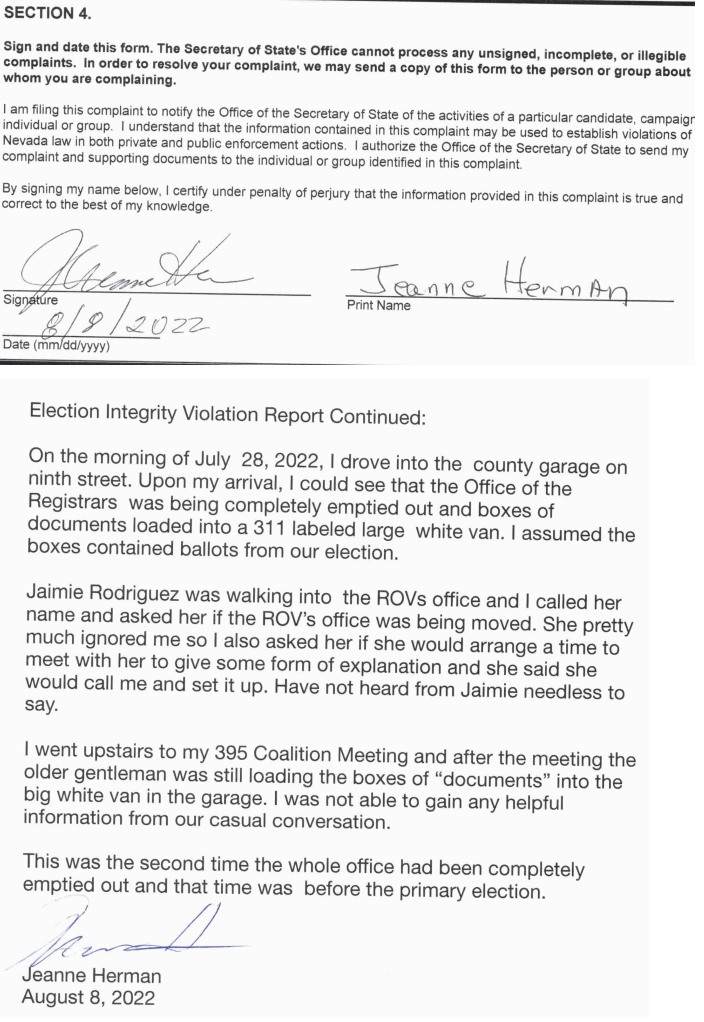
\includegraphics[width=280pt]{Herman Aff.png}}
\end{figure}

\newpage
\subsection{Clark County 2020 and 2022 Tabulation Sources}
2020 General Election:\url{https://www.clarkcountynv.gov/government/departments/elections/past_elections.php}

Now let's examine the State Law on how the ballots are counted.

2020 Presidential Election:\url{https://elections.clarkcountynv.gov/electionresults/sov/20G/PRESIDENT.txt}

2022 Attorney General:\url{https://elections.clarkcountynv.gov/electionresults/sov/22G/ATTORNEY%20GENERAL.txt}

2022 Secretary of State:\url{https://elections.clarkcountynv.gov/electionresults/sov/22G/SECRETARY%20OF%20STATE.txt}

2022 Dem Gov Primary:\url{https://elections.clarkcountynv.gov/electionresults/sov/22P/GOVERNOR%20-%20DEM.txt}

2022 Rep  Gov Primary:\url{https://elections.clarkcountynv.gov/electionresults/sov/22P/GOVERNOR%20-%20REP.txt}

\subsection{Washoe County 2020 and 2022 Tabulation Sources}
2020 General Election: \url{https://www.washoecounty.gov/voters/old-site/elections/past-election-information/electionresults/2020generalelectionresults.php}

2022 Primaries: \url{https://www.washoecounty.gov/voters/old-site/elections/past-election-information/electionresults/2022primaryelectionresults.php}

The 2022 CVR must be used to reconstruct the precinct level data by counting group for the 2022 Primaries.

Here is a link to the CVR (cast vote record) compiled tabulations for Gilbert, Lombardo and Sisolak: \url{https://docs.google.com/spreadsheets/d/15N-l6Fd8iaZ9ZMt70b3wFTY5dccEyVf2rq_dZMRXevM/edit?usp=sharing}

Since the Precinct Level Results By Counting Group are not readily available for the 2020 Election, they had to be obtained directly in private communication with the Washoe
County Recorder (who didn't even have them, they first had to petition Dominion months after the election). On page four is proof of the communication that resulted in the release of the Precinct Level Counting Group results. 
\newpage
For the 2022 General Election, the CVR, which is has not yet been made available on their website, was sequestered via direct communication with the Registrar of Voters. Here is 
the link to the CVR in Excel:\url{https://docs.google.com/spreadsheets/d/1bE-iKZSz-JCtakk7DjEbKE1bT7KFpSHzLNhb6VtvzSA/edit?usp=sharing}

2020 Washoe Precinct Results by Counting Group, as provided by the Washoe County Clerk’s Office:\url{https://docs.google.com/spreadsheets/d/1TtybEsLhRHQIAJ_TWtdF54w4_77LZWyV/edit?usp=sharing&ouid=100231490512233358920&rtpof=true&sd=true}

This is the spreadsheet of the combined county tabulations that we shall be using for the remainder of this article: Nevada 2020, Clark and Washoe Tabulations:\\ \url{https://docs.google.com/spreadsheets/d/1gkf41sJRAQ6bwKmlAAcb7hAQ6v4zIXG2wDYl67LrJ4k/edit?usp=sharing}

 The second tab in the above spreadsheet contains 1075 of the 1286 precincts. These are the precincts that meet the arbitrary criterion of having no less than 50 ballots cast in each counting group.
 
If any precinct in any of the four counting groups (Trump Early, Biden Early, Trump Mail and Biden Mail) reported less than 50 ballots cast, then that precinct was excluded from the official analysis in order to ensure that the decimal resolution of the division of any two counting groups is at least $1\%$, and that the decimal resolution of any counting group divided by the total number of ballots cast in all four groups is at least $0.5\%.$

Of these 1075 precincts, an additional three precincts were removed for outstanding outlying behavior, reducing the final count of analyzed precincts from 1075 to 1072.

It is the inability to either locate official tabulation sources (by counting group) or to access them in a usable form (such as spreadsheet), that acts as the greatest barrier to detailed election analysis.

One would think that the public would have immediate access to the tabulation results of their own county, including a breakdown of Election Day, Mail-in and Early Voting per precinct. 

Nay, this is actually not the case---thus it is very frustrating to procure such data across the United States, and often impossible. And when such data sources can be procured, one must then put that data in a usable form (most sources provided by the County are in PDF form, such that each relevant entry must be placed manually by hand into a spreadsheet!)
\newpage
\begin{figure}
\caption{Proof of Communication with Washoe County Recorder}
    \centering
    \makebox[0pt]{%
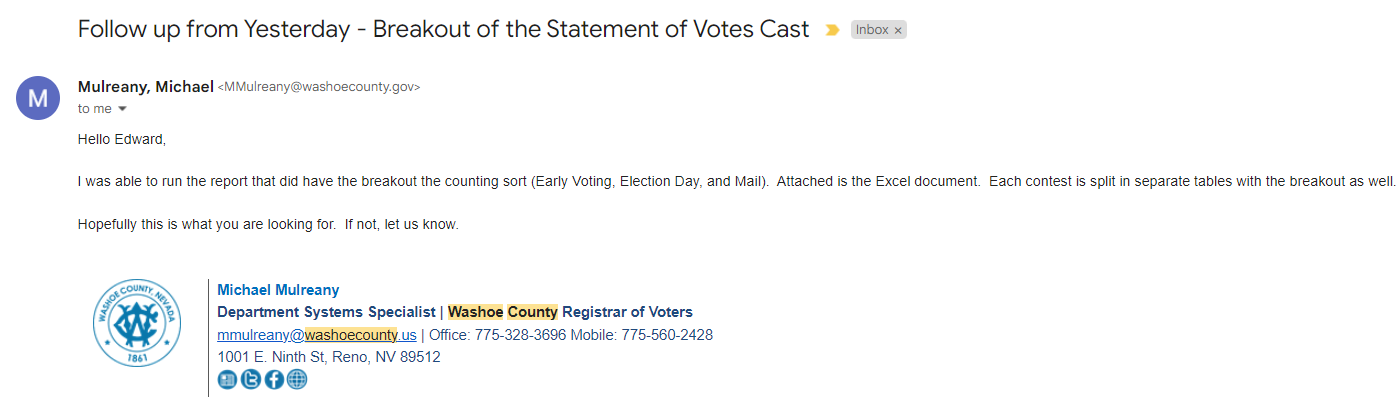
\includegraphics[width=0.9\paperwidth]{Washoe County Recorder.png}}
\end{figure}

Before we proceed to the main body of this article, I decided to query ChatGPT for its opinion of the following question before writing and submitting this article for publication, below is the link to this conversation:
\url{https://chat.openai.com/share/f72a566c-cdb0-47f0-ab3f-3146f7e3c109}

``Let A be Alice's Early Vote, B be Bob's Early Vote, C be Alice's Mail-in Vote and D be Bob's Mail-in Vote at a particular precinct. Also, let N be the sum of A,B, C and D, which is the sum of all ballots cast at the precinct.

Would it be unusual for a dataset of over 1000 precincts, from two different geographic regions (one urban and one suburban) on different sides of the same State (such as Clark and Washoe Counties in Nevada), for there to be a strong linear regression from N and A onto D (that is, with the $R^2$ of the regression exceeding 0.98), allowing someone to predict D knowing only N and A?”

The response:

``If there is a dataset of over 1000 precincts from two different geographic regions (one urban and one suburban) on different sides of the same State (such as Clark and Washoe Counties in Nevada), and there is a strong linear regression with an $R^2$ exceeding 0.98 between the variables N (the sum of A, B, C, and D) and A (Alice's Early Vote) onto D (Bob's Mail-in Vote), it would be unusual and raise concerns about the authenticity and integrity of the data.

A high $R^2$ value suggests a strong relationship between the predictor variables (N and A) and the response variable (D). In this case, it would indicate that knowing the sum of all ballots cast (N) and Alice's Early Vote (A) would allow for accurate predictions of Bob's Mail-in Vote (D). Such a strong relationship could imply a pattern or correlation \textbf{that is not expected in a fair and unbiased voting process.}

In a democratic election, the votes cast by different individuals should be independent and not significantly influenced by external factors \textbf{such as the total number of votes or the votes cast by other individuals}. Therefore, if there is a strong linear regression allowing precise predictions of Bob's Mail-in Vote based on N and A, \textbf{it could raise concerns about potential anomalies, manipulation, or non-authentic behavior within the dataset.}

In such cases, \textbf{further investigation and analysis would be \textcolor{red}{necessary}} to understand the underlying reasons for this relationship and determine whether any irregularities or biases have affected the voting process."

Although I personally believe that such evidence is sufficient to convince a Jury in a Court of Law to rule the 2020 and 2022 Nevada election a fraud, nevertheless further investigation is indeed necessary before a definitive conclusion can be reached.

Unfortunately, a spreadsheet of tabulations does not provide us with the means to investigate the issue any further, nor is the source code of voting software publicly available; thus, only the authorities themselves can carry out a further investigation of these facts and how they occurred.

I do however concur with the response given by ChatGPT that indeed such a further investigation is \textcolor{red}{necessary} to ascertain how this result could occur in a purported ``safe and secure election."

For this reason, I authorize the journal to accept additional co-authors with either concurrent or dissenting opinions.

However, in order to ensure that the conversation remains balanced, I only authorize one dissenting opinion per one concurrent opinion (including my own); thus if no other concurrent opinions are added to this article, then only one dissenting opinion is permitted.

It is entirely up to the intellectual capacity and critical reading skills of the reader to discern those things which are absolute mathematical fact and those that are opinion. 

That is, anything that I say that cannot be strictly written in a mathematical form, is indeed opinion; however, I am certain that these ``opinions" would be ``made facts" in a Court of Law if brought before a Jury. Woe to the ``expert" that has to defend a constant ratio of ballot counts across the precincts of two distant counties.

\newpage
\section{The Twenty Laws and Forty Isometries That Govern the Proportion Between Four Disjoint Sets}
In most elections across the United States, there are only two major candidates, one of the Democrat Party and one of the Republican Party. By Law, no voter may vote more than once, nor may vote for more than one candidate (excluding races which permit multiple candidate selection).

As such, at any particular voting station (precinct), the set of ballots cast for each nominee are mathematically disjoint; furthermore, that the set of ballots for each counting group and each nominee (such as Republican Early, Republican Mail-in, Democrat Early and Democrat Mail-in) as also mathematically disjoint.

Because they are disjoint, the ratios between any four non-empty disjoint subsets from any number of disjoint counting groups for the same race (that is, we cannot mix the ballots from different races at the same precinct) are beholden to the sixty mathematical tautologies found in \textbf{Definition 1.2}.

The following definitions assume a rigid referential system, this system being the four quadrants of square. I shall describe in plain English the real life scenario which gives birth to the figure on page 21.

Suppose that there is an election occurring inside of a High School gym. 

The Trump Early Ballots are placed in the Northwest corner, the Biden Early Ballots are placed in the Northeast Corner. Thus, all early ballots reside solely within the Northern Half of the gymnasium.

In order to retain a clockwise relationship between the vote ratios, we now place Trump's Mail-in ballots in the Southeast Corner (diagonally across from Trump's Early ballots in the Northwest); likewise, we place Biden's Mail-in Ballots in the Southwest Corner (which are diagonally across from Biden's Early ballots in the Northeast). Thus, all of the Mail-in ballots reside solely within the Southern Half of the Gym.

Having the counting groups placed in these four quadrants allows to rapidly switch between the relationships of any pairing of quadrants via isometric formulation; while maintaining the rigidity of referential system (in other words, Trump's Early ballots will always physically remain in the Northwest Corner, regardless of how we are analyzing the quadrants and their relationships; the same is also true for the other ballot types).

The first quadrant pairings that we analyze are the Northern Quadrant Pair vs the Southern Quadrant Pair, which is the Early Vote vs the Mail-in Vote. This is the natural way that one would approach an election, hence the North vs South paradigm is the called the ``Standard Orientation."
\newpage
The second quadrant pairings that we would naturally analyze are the Diagonal pairings, which would be Republican Early Vote and the Republican Mail-in Vote, vs, the Democrat Early Vote and Democrat Mail-in Vote. In this orientation we comparing Republican voters against themselves (the ratio of Republicans that preferred to vote early as opposed to by mail); likewise we are also comparing Democrats against themselves (the ratio of early vs mail-in preference), and when the two diagonals are contrasted against each other, we are contrasting the preference of both parties to vote Early or by Mail.

Thus the Diagonal vs Diagonal Paradigm is called the Preference Orientation, as it allows us to contrast the preferred type of ballot casting both within the same party and between parties.

Before I discuss the third orientation (West vs East), let's start with the first and second orientations. In the figure on page nine you shall see the Standard Orientation of Early vs Mail-in (North vs South). Within this gym (precinct), let $s,t,u,v$ be Trump's Early, Biden's Early, Trump's Mail-in Vote and Biden's Mail-in Vote (respectively).

Trump's Early Percentage is denoted as $x=\frac{s}{s+t}$; Trump's Mail-in Percentage is denoted as $y=\frac{u}{u+v}$.

The last natural parameter in this orientation is the Proportion of Mail-in to Election Day Ballots, zeta, where $\zeta=\frac{u+t}{s+t}$. In a fair election, some people choose to cast their ballots Early, and other prefer to cast them via mail. 

Amongst those two groups, some will choose to vote Republican and others will choose to vote Democrat; hence, although there may be (and is expected to be) strong correlations between Trump's Early Percentage, Trump's Mail-in Percentage and the Proportion of Mail-in to Election Day Votes across a set of precincts, they generally operate independent of each other.

Whereas Trump's total percentage of \textbf{all ballots cast} at the precinct \textbf{cannot be known until all ballots are cast!} The Early Vote is one event, and the Mail-in Vote is another event, and the proportion of those that participated in either event is the timeless relationship between the Early Vote and Mail-in Vote. The combined action of these events yields Trump's Total Percentage, thus the Early Vote and the Mail-in Vote are the \textbf{Cause} and Trump's Total Percentage is the \textbf{Effect}.

Thus, when we have deterministic formulas that allow us to deduce Trump's Mail-in Percentage from Trump's Total Percentage and his Early Percentage, without needing to know the Proportion of Mail-in to Election Day Votes, then something is clearly wrong with the \textbf{Arrow of Time}.  How could Trump's Total Percentage be the \textbf{Cause} of his Mail-in Percentage?
\newpage
Likewise, how could Biden's Mail-in Vote be the \textbf{effect} of the Total Ballots Cast and Trump's Early Vote (like in Clark and Washoe Counties in 2020)?

Under no circumstance does it make sense that we can predict Biden's Early Vote knowing only the Total Ballots Cast and Trump's Early Vote, with no knowledge of Trump's Mail-in Vote or Biden's Early Vote, for such a relationship implies that the Early and Mail-in Votes have forfeit their general independence, and somehow a future event (the total ballots cast) became the \textbf{cause} of Biden's Mail-in Vote, instead of Biden's Mail-in Vote being one of the four independent events that \textbf{caused} the total ballots cast.

Now you may say ``correlation is not causation," but let's get real here, we're talking about an election with four time-dependent events. We can predict Biden's Mail-in Vote with an $R^2>0.985$ with a simple plane equation of the Total Ballots Cast and Trump's Early Vote; likewise we can invert this plane equation in order to yield Total Ballots Cast from Trump's Early Vote and Biden's Mail Vote, or Trump's Early vote from Total Ballots Cast and Biden's Mail-in Vote...all of which are absurd, since the relationship disavows the natural time dependency of the events in question, whilst also completely disregarding Trump's Mail-in Vote and Biden's Early Vote.

Nay, this is not just a high correlation, but indeed causation: The \textbf{Cause} being a Rigged Election.

Let us now return our attention to the diagram on page nine: Trump's Percentage of all ballots (which shall heretofore call Trump's Aggregate Percentage) is denoted $\alpha=\frac{s+u}{(s+u)+(t+v)}$. 

There is second aggregate percentage: The percentage of all ballots cast that are Election Day Ballots, we shall call this Omega, which as a direct identity with zeta, viz. $\Omega=\frac{s+t}{(s+t)+(u+v)}; \Omega=\frac{1}{\zeta+1}; \zeta=\frac{1-\Omega}{\Omega}$. Although both entities (Omega and zeta), contain the same information, their usage and geometric meaning manifest different.

For instance, the aggregate percentage is written as a weighted sum of $x$ and $y$, which invokes Omega in its simplest form: $\alpha=x\Omega+(1-\Omega)y$. However we could also write: $\alpha=\frac{x+\zeta y}{\zeta+1}$, but this form has no geometric meaning, especially since the denominator is equivalent to Omega, ie. $\alpha=\frac{x+\zeta y}{\zeta+1}=\frac{1}{\zeta+1}(x+\zeta y)$.

However, if we attempt to solve for $x$, it is the other way around. Now we must invoke zeta in order for the description of $x$ to have meaning: $$x=\alpha+\zeta(\alpha-y)$$
This equation states that $x$ is the reflection of $y$ over the value of $\alpha$ by a length equal to the distance from the reflector ($\alpha$) to image ($y$) scaled by $zeta$.
\newpage
Using Omega to describe $x$, we yield:
$x=\frac{\alpha-(1-\Omega)y}{\Omega}$

There is simply no way to rationalize the above equation in plain English, because it not how Mother Nature herself would represent $x$. Hence, even though Omega and zeta contain the same information, there is a proper time and place for invocation of either---but never both simultaneously. More specifically, where $\cos(\theta)=\sqrt{\Omega}$ and $\sin(\theta)=\sqrt{1-\Omega}$ and $\tan(\theta)=\sqrt{\zeta}$:
$$\alpha=x\cos^2(\theta)+y\sin^2(\theta)=\frac{x+y\tan^2(\theta)}{1+\tan^2(\theta)}=\frac{x+y\tan^2(\theta)}{sec^2(\theta)}$$ 
$$\alpha=\frac{x+y\tan^2(\theta)}{1+\tan^2(\theta)} \implies x=\alpha+\alpha\tan^2(\theta)-y\tan^2(\theta)=\alpha+\tan^2(\theta)(\alpha-y)$$


Finally, there is a third aggregate percentage. This percentage is called Lambda, and represents the percentage of ballots cast that are on the West Side of square. Thus $\lambda=\frac{s+v}{(s+v)+(u+t)}$.

In a fair election we would never consider an entity such as $\lambda$, because no one would think to examine the relationship of Trump's Early Vote and Biden's Mail-in Vote vs Trump's Mail-in Vote and Biden's Early Vote, because $\lambda$ does not describe a particular behavior or preference of the electorate. Lambda is also known as the ``Obstacle Percentage." 

I shall elaborate more upon why this is the ``Obstacle Percentage in Section 1.13 of this Chapter, titled ``The Geometric Absurdity of Constant Lambda." 

However, to summarize the issue for the time being, that if $\lambda$ has constant value across the precincts (a consistent mean with a small standard deviation, like in Nevada), such as $\lambda=65\%$ across the precincts (the real average is 63.5\%, but I'm keeping it multiples of 5\% for easy reading), it means that Trump needs to get 65\% of the Election Day Vote before he can get more the 35\% of the Mail-in Vote, because Biden's Mail-in Percentage, is the reflection of Trump's Election Day Percentage, over the reflector, $\lambda$, scaled by $\zeta^{1}=\frac{\Omega}{1-\Omega}$. 

Thus if Lambda is sitting at 65\% across the precincts, then Biden's Mail-in Percentage cannot fall below 65\% (meaning Trump's Mail-in Percentage cannot exceed 35\%) until Trump acquires at least 65\% of the Election Day Vote---hence constant lambda is an \textbf{tremendous obstacle} to Republicans if $\lambda>55\%$ across the precincts and an obstacle to Democrats if $\lambda<45\%$ across the precincts.

\begin{figure}[bp!]
\begin{center}
\caption{The High School Gymnasium Election Event}
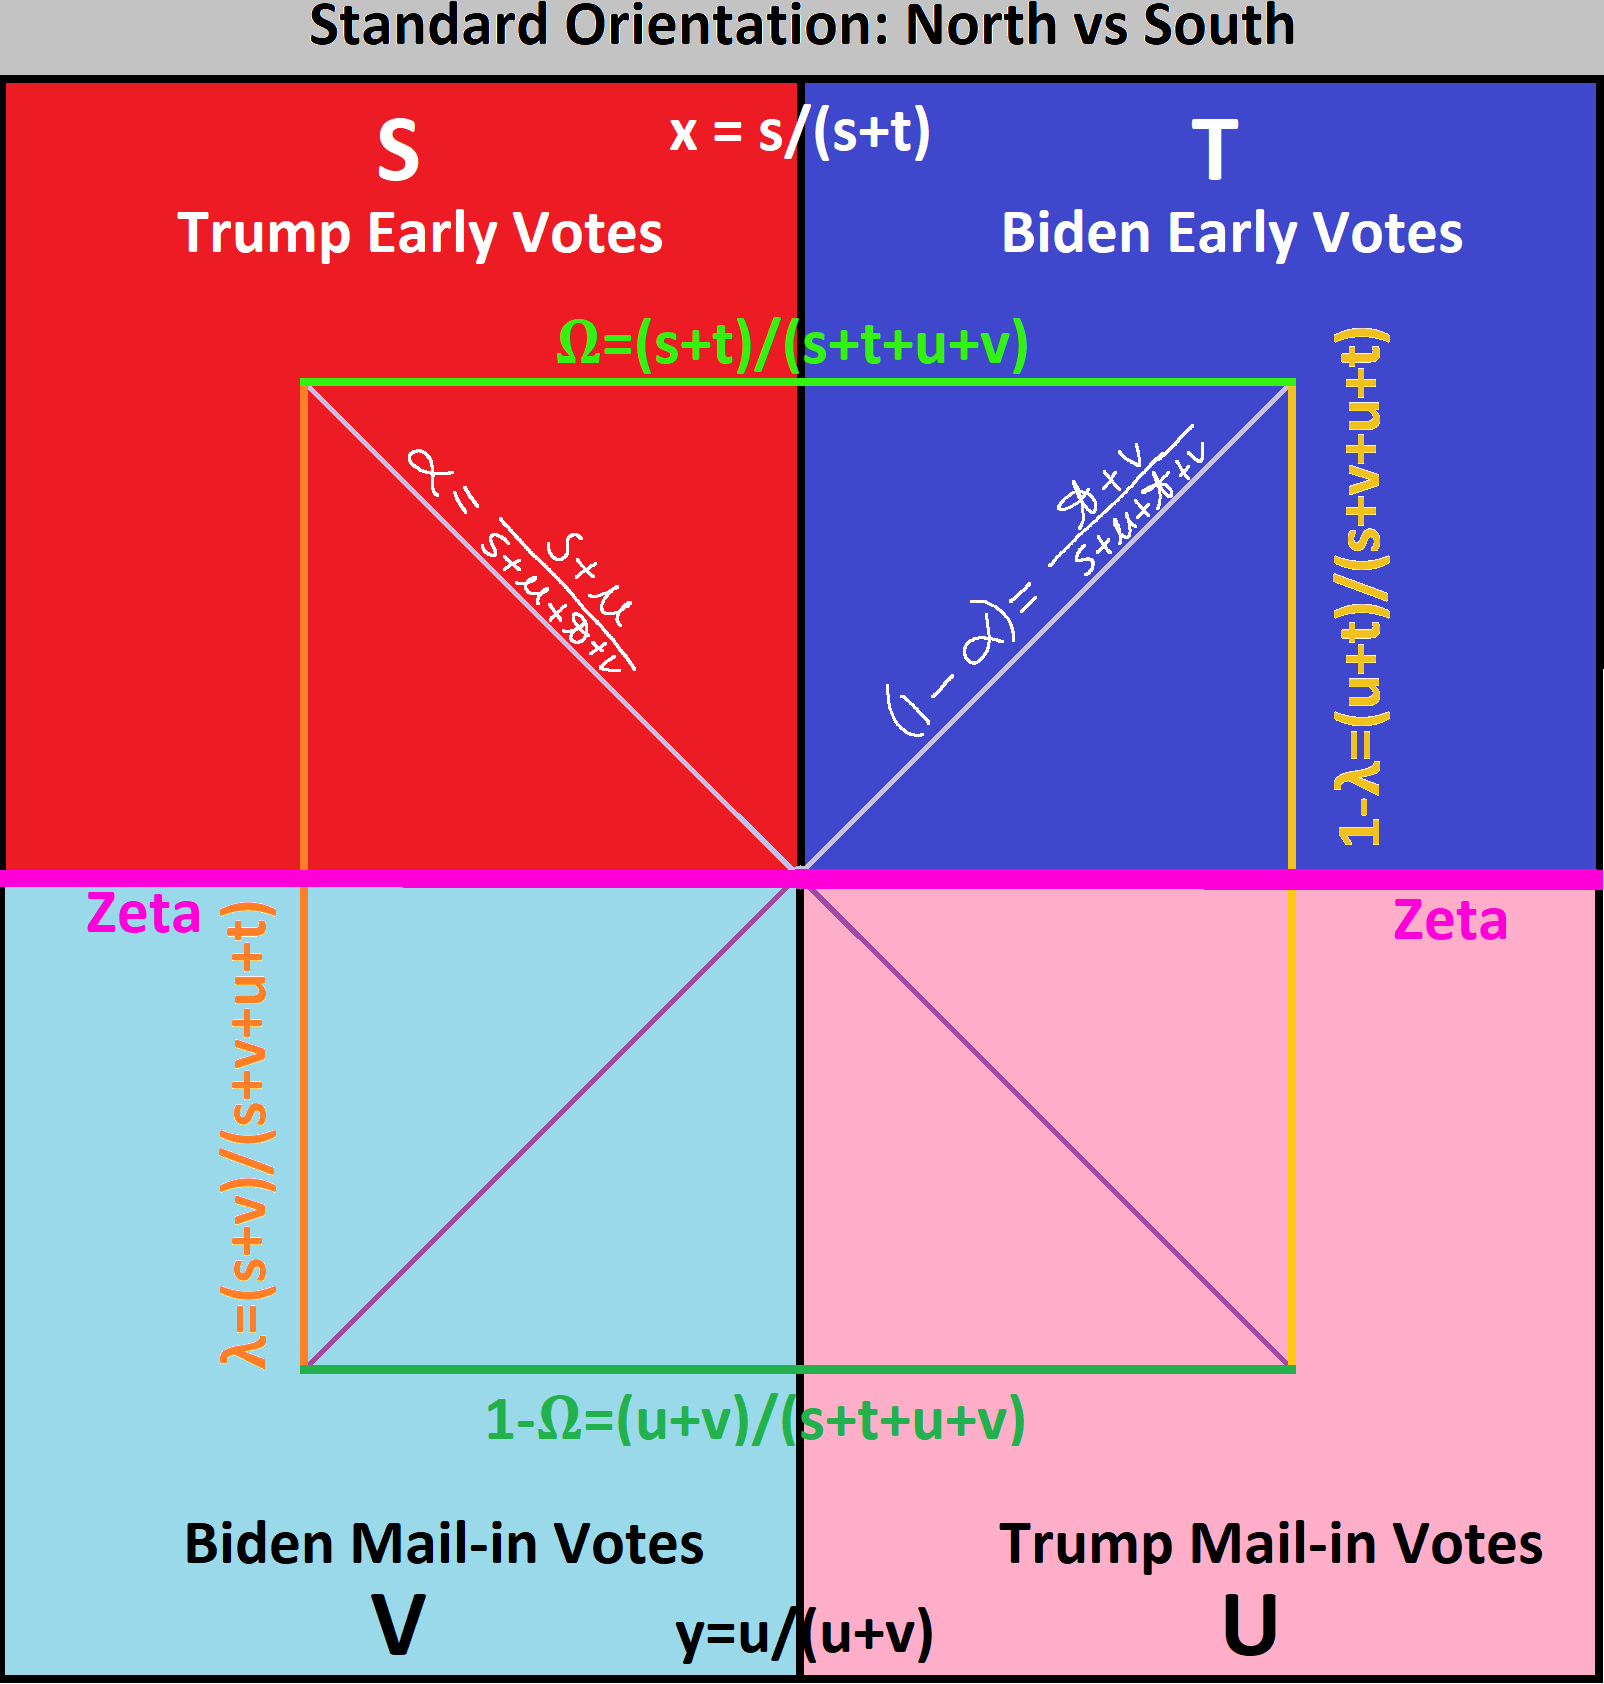
\includegraphics[width=265pt]{North vs South.png}
\end{center}
\end{figure}
\newpage
\subsection{The Ratios Between the of Cardinalities Four Pairwise Disjoint Sets}
\begin{definition}
Let \textbf{S,T,U,V} be four pairwise disjoint sets, such that $|S|,|T|,|U|,|V|$ equal $s,t,u,v$ respectively. Each ratio has a conserved partner which makes it easier to write the Laws that follow. They are conserved since they sum to 1 or 100\%, ie, $1=x_{1}+x_{2}$).

Each pair of lines in the below tables declares the written name of the ratio, as well as the quantitative definition.
\end{definition}
\SetTblrInner{rowsep=5pt,colsep=2pt}
\begin{tblr}{|l|l|l|l|}
\hline
North Ratio & South Ratio & North Complement & South Complement\\
\hline
$x_{1}=\frac{s}{s+t}$ & $y_{1}=\frac{u}{u+v}$ & $x_{2}=(1-x_{1})=\frac{t}{s+t}$  & $y_{2}=(1-y_{1})=\frac{v}{u+v}$\\
\hline
West Ratio & East Ratio & West Complement & East Complement\\
\hline
$g_{1}=\frac{s}{s+v}$ & $h_{1}=\frac{u}{u+t}$ & $g_{2}=(1-g_{1})=\frac{v}{s+v}$ & $h_{2}=(1-h_{1})=\frac{t}{u+t}$\\
\hline
Northwest Ratio & Northeast Ratio & Southeast Ratio & Southwest Ratio\\
\hline
$m_{1}=\frac{s}{s+u}$ & $n_{1}=\frac{t}{t+v}$ & $m_{2}=(1-m_{1})=\frac{u}{s+u}$ & $n_{2}=(1-n_{1})=\frac{v}{t+v}$\\
\hline
Diagonal Aggregate & Diagonal Proportion & 1st Alpha Identity & Xi Identity\\
\hline
$\alpha_{1}=\frac{s+u}{(s+u)+(t+v)}$ & $\xi=\frac{t+v}{s+u}$ & $\alpha_{1}=(\xi+1)^{-1}$ & $\xi=\frac{1-\alpha_{1}}{\alpha_{1}}=\frac{\alpha_{2}}{\alpha_{1}}$\\
\hline
Diagonal Complement & Diagonal Inverse & 2nd Alpha Identity & Inverse Xi Identity\\
\hline
$\alpha_{2}=\frac{t+v}{(s+u)+(t+v)}$ & $\xi^{-1}=\frac{s+u}{t+v}$ & $\alpha_{2}=(\xi^{-1}+1)^{-1}$ & $\xi^{-1}=\frac{1-\alpha_{2}}{\alpha_{2}}=\frac{\alpha_{1}}{\alpha_{2}}$\\
\hline
West Aggregate & East to West Proportion & 1st Lambda Identity & Gamma Identity\\
\hline
$\lambda_{1}=\frac{s+v}{(s+v)+(u+t)}$ & $\gamma=\frac{u+t}{s+v}$ & $\lambda_{1}=(\gamma+1)^{-1}$ & $\gamma=\frac{1-\lambda_{1}}{\lambda_{1}}=\frac{\lambda_{2}}{\lambda_{1}}$\\
\hline
East Aggregate & West to East Proportion & 2nd Lambda Identity & Inverse Gamma Identity\\
\hline
$\lambda_{2}=\frac{u+t}{(s+v)+(u+t)}$ & $\gamma^{-1}=\frac{s+v}{u+t}$ & $\lambda_{2}=(\gamma^{-1}+1)^{-1}$ & $\gamma^{-1}=\frac{1-\lambda_{2}}{\lambda_{2}}=\frac{\lambda_{1}}{\lambda_{2}}$\\
\hline
North Aggregate & South to North Proportion & 1st Omega Identity & Zeta Identity\\
\hline
$\Omega_{1}=\frac{s+t}{(s+t)+(u+v)}$ & $\zeta=\frac{u+v}{s+t}$ & $\Omega_{1}=(\zeta+1)^{-1}$ & $\zeta=\frac{1-\Omega_{1}}{\Omega_{1}}=\frac{\Omega_{2}}{\Omega_{1}}$\\
\hline
South Aggregate & North to South Proportion & 2nd Omega Identity & Inverse Zeta Identity\\
\hline
$\Omega_{2}=\frac{u+v}{(s+t)+(u+v)}$ & $\zeta^{-1}=\frac{s+t}{u+v}$ & $\Omega_{2}=(\zeta^{-1}+1)^{-1}$ & $\zeta^{-1}=\frac{1-\Omega_{2}}{\Omega_{2}}=\frac{\Omega_{1}}{\Omega_{2}}$\\
\hline
\end{tblr}
\newpage
\subsection{The Twenty Laws and Forty Isometries}
\begin{definition}
\end{definition}
\SetTblrInner{rowsep=5pt,colsep=2pt}
\begin{tblr}{|l|l|l|l|}
\hline
Law Number & North vs South & West vs East & Diagonal vs Diagonal\\
\hline
First Law & $x_{1}=\alpha_{1}+\zeta(\alpha_{1}-y_{1})$ & $g_{1}=\alpha_{1}+\gamma(\alpha_{1}-h_{1})$ & $m_{1}=\Omega_{1}+\xi(\Omega_{1}-n_{1})$\\
\hline
Second Law & $x_{1}=\lambda_{1}+\zeta(\lambda_{1}-y_{2})$ & $g_{1}=\Omega_{1}+\gamma(\Omega_{1}-h_{2})$ & $m_{1}=\lambda_{1}+\xi(\lambda_{1}-n_{2})$\\
\hline
Third Law & $x_{1}=\frac{\alpha_{1}y_{2}-\lambda_{1}y_{1}}{(\alpha_{1}-\lambda_{1})-(y_{1}-y_{2})}$ & $g_{1}=\frac{\alpha_{1}h_{2}-\Omega_{1}h_{1}}{(\alpha_{1}-\Omega_{1})-(h_{1}-h_{2})}$ & $m_{1}=\frac{\Omega_{1}n_{2}-\lambda_{1}n_{1}}{(\Omega_{1}-\lambda_{1})-(n_{1}-n_{2})}$\\
\hline
Fourth Law & $x_{1}=\frac{\lambda_{1}+\alpha_{1}-\Omega_{2}}{2\Omega_{1}}$ & $g_{1}=\frac{\Omega_{1}+\alpha_{1}-\lambda_{2}}{2\lambda_{1}}$ & $m_{1}=\frac{\lambda_{1}+\Omega_{1}-\alpha_{2}}{2\alpha_{1}}$\\
\hline
Fifth Law & $y_{1}=\alpha_{1}-\zeta^{-1}(\alpha_{1}-x_{1})$ & $h_{1}=\alpha_{1}-\gamma^{-1}(\alpha_{1}-g_{1})$ & $n_{1}=\Omega_{1}-\xi^{-1}(\Omega_{1}-m_{1})$\\
\hline
Sixth Law & $y_{1}=\lambda_{2}-\zeta^{-1}(\lambda_{1}-x_{1})$ & $h_{1}=\Omega_{2}-\gamma^{-1}(\Omega_{1}-g_{1})$ & $n_{1}=\lambda_{2}-\xi^{-1}(\lambda_{1}-m_{1})$\\
\hline
Seventh Law & $y_{1}=\frac{x_{1}\lambda_{2}-x_{2}\alpha_{1}}{(\lambda_{2}-\alpha_{1})-(x_{2}-x_{1})}$ & $h_{1}=\frac{g_{1}\Omega_{2}-g_{2}\alpha_{1}}{(\Omega_{2}-\alpha_{1})-(g_{2}-g_{1})}$ & $n_{1}=\frac{m_{1}\lambda_{2}-m_{2}\Omega_{1}}{(\lambda_{2}-\Omega_{1})-(m_{2}-m_{1})}$\\
\hline
Eighth Law & $y_{1}=\frac{\lambda_{2}+\alpha_{1}-\Omega_{1}}{2\Omega_{2}}$ & $h_{1}=\frac{\Omega_{2}+\alpha_{1}-\lambda_{1}}{2\lambda_{2}}$ & $n_{1}=\frac{\lambda_{2}+\Omega_{1}-\alpha_{1}}{2\alpha_{2}}$\\
\hline
Ninth Law & $\alpha_{1}=x_{1}\Omega_{1}+\Omega_{2}y_{1}$ & $\alpha_{1}=g_{1}\lambda_{1}+\lambda_{2}h_{1}$ & $\Omega_{1}=m_{1}\alpha_{1}+\alpha_{2}n_{1}$\\
\hline
Tenth Law & $\alpha_{1}=\Omega_{1}(x_{1}-x_{2})+\lambda_{2}$ & $\alpha_{1}=\lambda_{1}(g_{1}-g_{2})+\Omega_{2}$ & $\Omega_{1}=\alpha_{1}(m_{1}-m_{2})+\lambda_{2}$\\
\hline
Eleventh Law & $\alpha_{1}=\Omega_{2}(y_{1}-y_{2})+\lambda_{1}$ & $\alpha_{1}=\lambda_{2}(h_{1}-h_{2})+\Omega_{1}$ & $\Omega_{1}=\alpha_{2}(n_{1}-n_{2})+\lambda_{1}$\\
\hline
Twelfth Law & $\alpha_{1}=\frac{x_{1}(y_{2}-y_{1})-\lambda_{1}(x_{1}-y_{1})}{y_{2}-x_{1}}$ & $\alpha_{1}=\frac{g_{1}(h_{2}-h_{1})-\Omega_{1}(g_{1}-h_{1})}{h_{2}-g_{1}}$ & $\Omega_{1}=\frac{m_{1}(n_{2}-n_{1})-\lambda_{1}(m_{1}-n_{1})}{n_{2}-m_{1}}$\\
\hline
Thirteenth Law & $\lambda_{1}=x_{1}\Omega_{1}+\Omega_{2}y_{2}$ & $\Omega_{1}=g_{1}\lambda_{1}+\lambda_{2}h_{2}$ & $\lambda_{1}=m_{1}\alpha_{1}+\alpha_{2}n_{2}$\\
\hline
Fourteenth Law & $\lambda_{1}=\Omega_{1}(x_{1}-x_{2})+\alpha_{2}$ & $\Omega_{1}=\lambda_{1}(g_{1}-g_{2})+\alpha_{2}$ & $\lambda_{1}=\alpha_{1}(m_{1}-m_{2})+\Omega_{2}$\\
\hline
Fifteenth Law & $\lambda_{1}=\frac{\alpha_{1}(x_{1}-y_{2})-x_{1}(y_{1}-y_{2})}{x_{1}-y_{1}}$ & $\Omega_{1}=\frac{\alpha_{1}(g_{1}-h_{2})-g_{1}(h_{1}-h_{2})}{g_{1}-h_{1}}$ & $\lambda_{1}=\frac{\Omega_{1}(m_{1}-n_{2})-m_{1}(n_{1}-n_{2})}{m_{1}-n_{1}}$\\
\hline
Sixteenth Law & $\lambda_{1}=\Omega_{2}(y_{2}-y_{1})+\alpha_{1}$ & $\Omega_{1}=\lambda_{2}(h_{2}-h_{1})+\alpha_{1}$ & $\lambda_{1}=\alpha_{2}(n_{2}-n_{1})+\Omega_{1}$\\
\hline
Seventeenth Law & $\zeta=\frac{x_{1}-\alpha_{1}}{\alpha_{1}-y_{1}};\Omega_{1}=\frac{y_{1}-\alpha_{1}}{y_{1}-x_{1}}$ & $\gamma=\frac{g_{1}-\alpha_{1}}{\alpha_{1}-h_{1}};\lambda_{1}=\frac{h_{1}-\alpha_{1}}{h_{1}-g_{1}}$ & $\xi=\frac{m_{1}-\Omega_{1}}{\Omega_{1}-n_{1}};\alpha_{1}=\frac{n_{1}-\Omega_{1}}{n_{1}-m_{1}}$\\
\hline
Eighteenth Law & $\Omega_{1}=\frac{\lambda_{2}-\alpha_{1}}{x_{2}-x_{1}}=\frac{\alpha_{2}-\lambda_{1}}{x_{2}-x_{1}}$ & $\gamma_{1}=\frac{\Omega_{2}-\alpha_{1}}{g_{2}-g_{1}}=\frac{\alpha_{2}-\Omega_{1}}{g_{2}-g_{1}}$ & $\alpha_{1}=\frac{\lambda_{2}-\Omega_{1}}{m_{2}-m_{1}}=\frac{\Omega_{2}-\lambda_{1}}{m_{2}-m_{1}}$\\
\hline
Nineteenth Law & $\zeta=\frac{x_{1}-\lambda_{1}}{\lambda_{1}-y_{2}}; \Omega_{1}=\frac{y_{2}-\lambda_{1}}{y_{2}-x_{1}}$ & $\gamma=\frac{g_{1}-\Omega_{1}}{\Omega_{1}-h_{2}}; \lambda_{1}=\frac{h_{2}-\Omega_{1}}{h_{2}-g_{1}}$ & $\xi=\frac{m_{1}-\lambda_{1}}{\lambda_{1}-n_{2}}; \alpha_{1}=\frac{n_{2}-\lambda_{1}}{n_{2}-m_{1}}$\\
\hline
Twentieth Law & $\zeta=\frac{\lambda_{1}-\alpha_{1}}{(y_{2}-y_{1})+(\alpha_{1}-\lambda_{1})}$ & $\gamma=\frac{\Omega_{1}-\alpha_{1}}{(h_{2}-h_{1})+(\alpha_{1}-\Omega_{1})}$ & $\xi=\frac{\lambda_{1}-\Omega_{1}}{(n_{2}-n_{1})+(\Omega_{1}-\lambda_{1})}$\\
\hline
\end{tblr}
\newpage
In the next figure we see the Diagonal vs Diagonal Orientation. For elections we call this the Preference Orientation, assuming that either diagonal contains ballots for the same candidate. 

The Republican Preference Percentage is the ratio of Republican Early ballots to all Republican ballots cast, that is which percentage of Republicans preferred to vote Early at the precinct, and is given by $m_{1}=\frac{s}{s+u}$. whereas its complement is the percentage of Republicans that preferred to vote by mail.

When the diagonals are constrained to the same candidate, then we call it the ``Northwest Preference Percentage" or the ``Republican Preference Percentage", otherwise we default to the name ``Northwest Ratio". Likewise, the other diagonal represents the ``Democrat Preference Percentage," or more generally the ``Northeast Ratio", given by $n_{1}=\frac{t}{t+v}$.

Since there is no way to visually divide the two sets of diagonal quadrants (while having both sets physically touching), a magenta hyperbola was used to represent the ratio of $\xi$, where $\xi$ is the ratio of all Democrat ballots to all Republican ballots, just as zeta is the ratio of all Northern Ballots to Southern ballots in the Standard Orientation.
\begin{figure}[bp!]
\begin{center}
\caption{The High School Gymnasium Election Event}
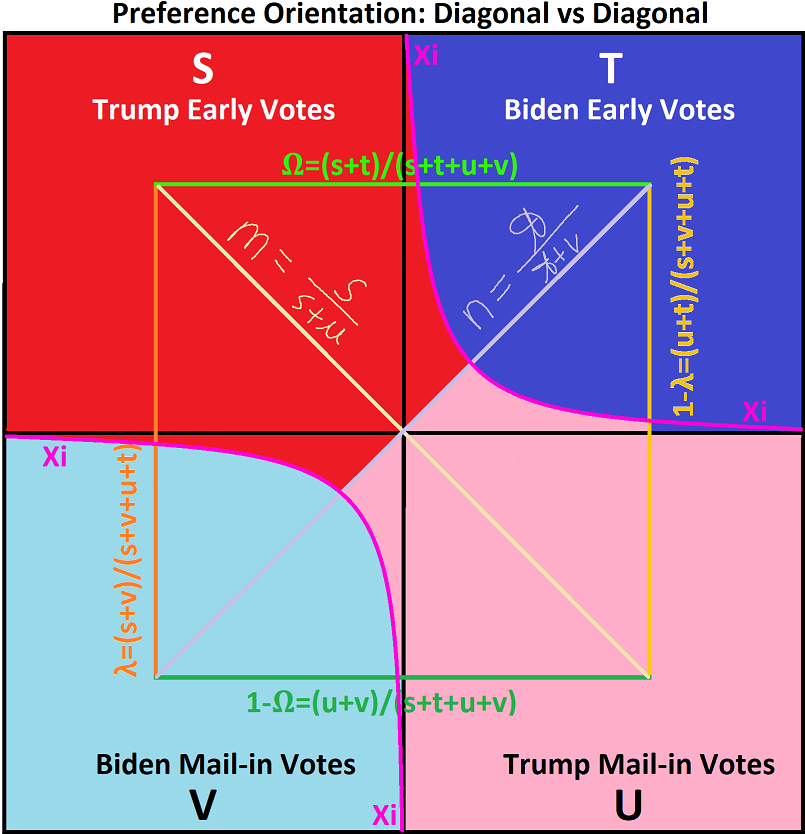
\includegraphics[width=265pt]{Diagonal vs Diagonal.png}
\end{center}
\end{figure}
\newpage
If we were to put Trump's and Biden's Early ballots in the same box, we label the box ``Early." Likewise if we then put the remaining ballots (Trump's and Biden's Mail-in ballots) in another box, we would label the box ``Mail-in." Both of these boxes would be the physical incarnation of the Standard Orientation (North vs South).

If we were to put Trump's Early and Mail-in ballots in the same box, we would label this box ``Republican" or ``Trump." Likewise if we then put the remaining ballots (Biden's Early and Mail-in ballots) in another box, we would label the box ``Democrat" or ``Biden." This would be the Preference Orientation (Diagonal vs Diagonal).

However, if were to put Trump's Early ballots and Biden's Mail-in ballots in the same box---how would we label the box? We can't, because there's no word in the English language that could describe this ballot mixture. 

Thus it is no wonder that the culprits behind this crime used this type of ballot mixture, because no one would even think to analyze such a thing. 

In fact, I only discovered the relationship by \textbf{accidentally} swapping the columns of Biden's Early and Mail-in votes in the spreadsheet I was using to analyze the Nevada elections. 

Yes, be it an act of my own clumsiness or an Act of G-d, it was only due to a lucky mistake in the spreadsheet column placement for Biden's Early and Mail-in ballots that I discovered the West vs East paradigm.

Once I was enlightened to mathematical existence of the ratios between these strange ballot mixtures, I immediately plotted the $g,h,\alpha$ coordinates of all the precincts of other counties in other States (such as Atlanta, GA; Chicago, IL) and not only did coordinates form a parametric surface, but eccentrically curved surfaces (unlike the flat plane formed by the $g,h,\alpha$ coordinates of Clark and Washoe Counties). If you go Georgia you get a quartic saddle, in Michigan you get a quadratic corkscrew, in Nevada a flat plane, in Maricopa a four dimensional cubic rollercoaster that uses the number of registered voters in its denominator (instead of ballots cast in the denominators), in Texas you get complex number vector manifolds that rig two elections at the same time! In fact, we even get a quaternionic vector manifold that rigged four statewide elections in Clark and Washoe Counties in the following cycle (2022 General Election).

Not only are the voters of these regions very creative in their manifold shapes and types, but they even took their artistry to unprecedented levels by invoking the quaternions. I am so glad that our elections are ``safe and secure," and that the common man has decided to collectively express their will through four-component vectors. Imagine how pleased Hamilton would be to know that his work is finally being appreciated and enjoyed throughout our nation!
\newpage
Let us now return our attention to the next figure on page 16. There is simply no label that we can assign to the West vs East paradigm, as such, we shall call it the ``Bastard Orientation."

In this orientation we are comparing Trump's Early Ballots and Biden's Mail-in ballots vs Trump's Mail-in Ballots and Biden's Early Ballots.

The percentage of ballots belonging to Trump on the west side is simply called ``Trump's West Side Ratio," which is given by $g=\frac{s}{s+v}$.

The percentage of ballots belonging to Trump on the east side is simply called ``Trump's East Side Ratio," which is given by $h=\frac{u}{u+t}$.

However, here comes the curious thing about this orientation (and it's this very thing that makes rigging elections in the West vs East paradigm so easy): The Proper Aggregate of this orientation is the exact same as the North vs South orientation; that is, $\alpha=x\Omega_{1}+\Omega_{2}y=g\lambda_{1}+\lambda_{2}h$.

Thus whether we are in the Standard (North vs South) or Bastard (West vs East) orientation, $\alpha$ remains the same, and represents the same thing geometrically in both Orientations, viz. Trump's Percentage of all Ballots Cast.

In the Bastard Orientation $\lambda$ becomes intuitive. It represents the percentage of all ballots that are on the West Side, and hence acts as the weight of the West Side Ratio, which is why its called the West Aggregate. 

Meanwhile the East Aggregate (which is $1-\lambda_{1}=\lambda_{2}$) is the percentage of all ballots cast that are on the east side, acting as the weight of the East Side Ratio; hence, $\alpha=g\lambda_{1}+\lambda_{2}h$.

The one thing that all of the ``Aggregate" percentages have in common is their denominator (which are equal to the total number of ballots cast); whereas the ratios between a quadrant pairing only have two totals in the denominator.
\newpage
Outside of the Bastard Orientation, there is no conceivable meaning to the West and East Aggregates. This is why the lambda ratio is not considered or examined in a fair a election, because its meaningless---people don't cast their ballots in Bastard Form.

Adam: ``Hey Bob, I'm voting for Trump after work at the Early Voting Center."

Bob: ``Damn...I was going to vote for Biden at the Early Voting Center---but since you're a Republican and you're going to the Early Voting Center---I'm going to send my Biden ballot via mail instead."

Although the above dialogue sounds ridiculous, this is exactly what it would mean if people cast their ballots in Bastard Form. It requires illicit communication of voter intent and illicit confirmation of candidate selection for the voters of a precinct to cast their ballots according to an equation written in the Bastard Form. 

This is why ChatGPT said: \textit{In a democratic election, the votes cast by different individuals should be independent and not significantly influenced by external factors \textbf{such as the total number of votes or the votes cast by other individuals}.}

Therefore, if there is a strong linear regression allowing precise predictions of Bob's Mail-in Vote based on N (Total Ballots Cast) and A (Alice's Early Vote), \textbf{it could raise concerns about potential anomalies, manipulation, or non-authentic behavior within the dataset.}

All of has been written in the previous few pages is exactly what ChatGPT was able to immediately deduce...exactly what any common man, with or \textbf{without a math degree, would be able to deduce.}

Thus, to any of those that are currently having dreams of writing a ``profound refutation of Edward Solomon's claims" know that it is not me that needs to be convinced, but the ordinary common man, who can utilize a handheld calculator to add Trump's Early Vote to Biden's Mail-in Vote and divide it by the total number of Early and Mail-in ballots cast, and keep getting the same ratio of 63.5\% with only a minuscule error.

If you do not believe you could deliver your ``profound refutation" to a jury of ordinary citizens with a straight face, then you ought not to write it, for even you do not believe in it.

\newpage
In Figure 5, below, we see the West vs East Orientation. The magenta line now runs vertically instead of horizontally as did in the North vs South Orientation, and it represents the proportion between the East and West sided ballots.

The Early Percentage (the north ratio) of $x=\frac{s}{s+t}$ has been replaced by the West Ratio of $g=\frac{s}{s+v}$.

The Mail-in Percentage (the south ratio) of $y=\frac{u}{u+v}$ has been replaced by the East Ratio $h=\frac{u}{u+t}$

Both ratios and their replacements retain the same term in their numerator, only exchanging their summands in the denominator.

Hence why the West vs East paradigm is so attractive for those who wish to do evil, as it retains its comparison of Candidate A vs Candidate B, while (as already mentioned) not being something that an honest person would ever consider analyzing.

Remember that I only discovered this paradigm by a miraculous accident of misplaced columns in a spreadsheet...what if I had not made ``mistake?"
\begin{figure}[bp!]
\begin{center}
\caption{The High School Gymnasium Election Event}
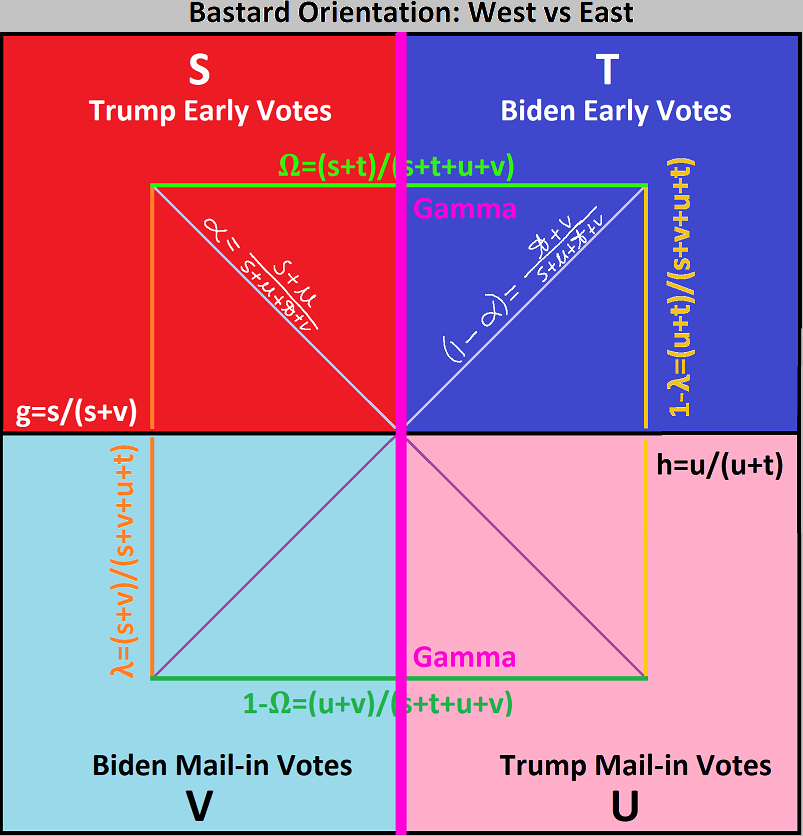
\includegraphics[width=250pt]{West vs East.png}
\end{center}
\end{figure}
\newpage
\subsection{The Importance of the Twenty Laws and Forty Isometries}

The Twenty Laws instruct us that is impossible for solve for any of Cardinality Ratios without knowing three other distinct Cardinality Ratios from the same orientation.

Let us examine the West vs East Isometry of the Ninth Law: $\alpha=g\lambda+\lambda_{2}h$.

It says that we require knowledge of $g,h$ and $\lambda$ in order to solve for $\alpha$, thus, if there exists a relationship between between any three of the four ratios, $\{g,h,\alpha,\lambda$\}, that allows us to solve for one of them knowing only the other two, with no knowledge of the remaining fourth ratio, then it is an indicator that something is wrong with the dataset (assuming its a dataset of concerning four distinct human behaviors, which are supposed to exhibit variability, instead of determinism).

In general, if any of the Twenty Laws (or their respective isometries) are violated, viz. the dataset allows us to predict any one of cardinality ratios with only one or two other cardinality ratios (from the same orientation), instead of three, then we have due cause to investigate the issue further.

The way in which I present the above paragraph to the general public is via the diagram below, which I have named the ``Fishtank Paradox."  Suppose you have two water tanks of equal width and height. One is filled to 25\% of its height, and the other to 75\% of its height. You then connect the two tanks with pipe and open the value, what will be the resultant equilibrium height?

Often they will answer 50\%, but then I show them that the question is impossible to answer, unless you know the ratio of their lengths. In the center image, the two tanks have the same length, so they do level out to 50\%; however, in the right image their lengths are in a One to Three proportion, so they level out to 62.5\%. Thus the diagram is a literal depiction of the Ninth Law.
\begin{figure}[bp!]
\begin{center}
\caption{The Layman's Example: The Fishtank Paradox}
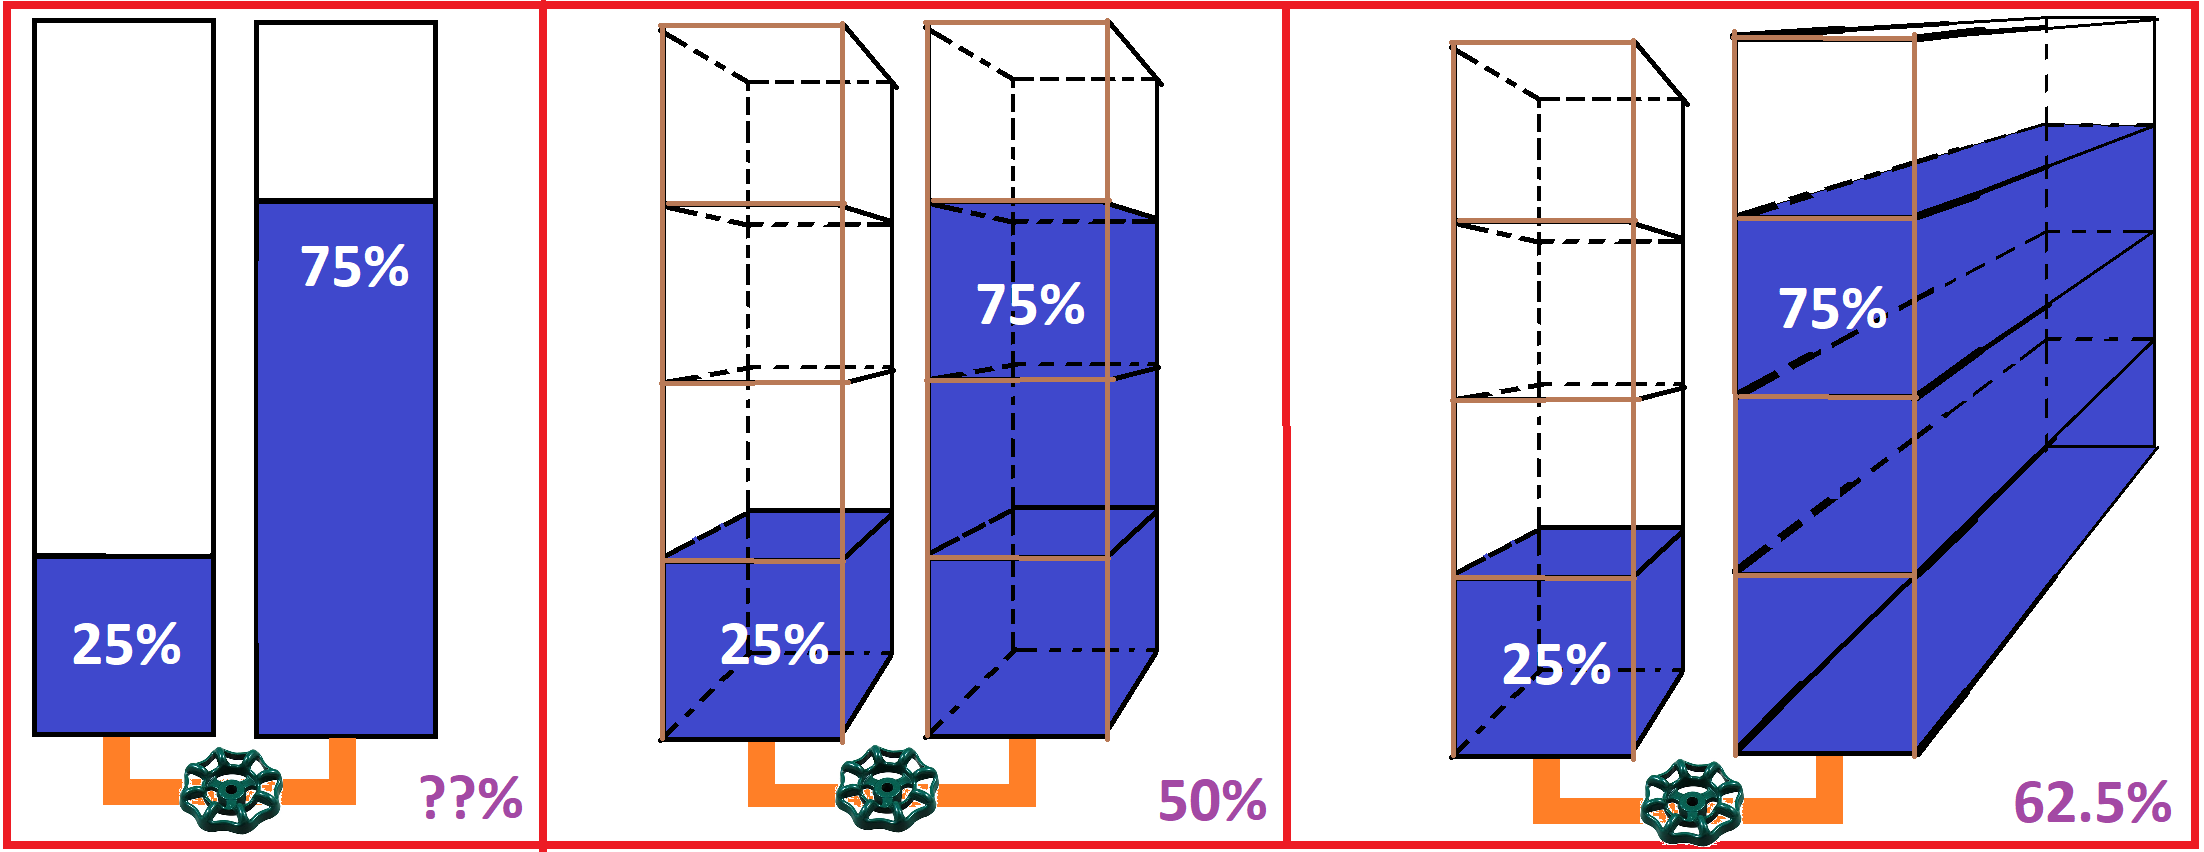
\includegraphics[width=350pt]{Fishtank.png}
\end{center}
\end{figure}

\newpage
\subsection{The Need for the Convergence, Constraint and Irrelevance Lemmas}
However there are trivial conditions under which finding a near deterministic relationship in a such a dataset would not be indicative of non-authentic human behavior.

As an example, suppose the average proportion of Mail-in to Early Votes was 20:1, then the aggregate percentage of any precinct would mostly be the same as the Mail-in Percentage, because the Early Vote is essentially non-existent compared to the Mail-in Vote.

Thus if found a strong linear regression from $x$ and $y$, being the Early and Mail-in Percentages for a candidate at a precinct, onto $\alpha$, being the candidate's aggregate percentage, it would not be surprising to see an $R^2$ exceeding 0.99, since $\alpha$ is approximately equal to $y$.

However, this would also imply that our ability to predict the Early Percentage, $x$, would be severely impaired, knowing only $alpha$ and $y$. Thus, if the proportion of Mail-in to Early votes was 20:1, and we could predict Early Percentage from the Mail-in Percentage and the Aggregate Percentage, with no knowledge of exact value of $\zeta$ (the proportion of Mail-in to Early Votes) at a precinct, then again, there would be a severe problem with the dataset.

Thus there exists a trade-off in predictive value concerning $x$ and $y$ at a precinct given knowledge of $\alpha$. This trade off depends upon the average value of $\Omega$ (or $\zeta$) across the dataset.  

As $\Omega$ goes to 0\%, then $\alpha$ rapidly approaches $x$ and our ability to predict $y$ rapidly degenerates (via the $R^2$ value of the prediction.

Likewise as $\Omega$ goes to 100\%, $\alpha$ approaches $y$ and our ability to predict $x$ rapidly degenerates.

Furthermore these trade-offs in predictive value also exist within the West vs East and Diagonal vs Diagonal orientations, exchanging $\{x,y,\Omega\}$ for either $\{g,h,\lambda\}$ or $\{m,n,\alpha\}$ (and exchanging $\alpha$ for $\Omega$ in the Diagonal vs Diagonal orientation).

In order to prevent the contents of this publication from being abused by others to falsely proclaim election fraud everywhere and anywhere, it is paramount to recognize and codify all trivial situations (starting in subsection 1.8) that would case manifold-like behavior in a fair election.
\newpage
\subsection{Tabulation Array; Data Set Definitions 1}

\begin{definition}{The Precinct Set and Principal Index}\\
Let \textbf{P} be a set of precincts and let them be sorted from least to greatest alphanumerically, such that $p_{w}$ is the $w^{th}$ precinct in the list. Let the first precinct in the list be the zeroth element (that is, we start with the zero index).

The assignment of ``w" to each precinct remains constant, even when the precincts are sorted by another parameters (or partitioned into different subsets). As such, ``w" is the Principal Index of any precinct no matter the immediate context, sorting or partitioning of \textbf{P}.

The function $\omega_{0}(p_{w})=w$, that is the lowercase omega function returns the zeroth (principal) index of any precinct.

Let the number of precincts in \textbf{P} be equal to $\beta_{0}$.

Precinct Data that does not originate from the County Recorder, Registrar of Voters or Secretary of State is 
\textcolor{red}{forbidden}, since it would declared \textcolor{red}{hearsay} in a Court of Law (such as the New York Times precinct .json time-series).
\end{definition}

\begin{definition}{The Race, Candidate and Mode Sets; Tabulation Tensor}\\
Let \textbf{R} be the set of Races being analyzed (that have two or more significant candidates, that only permit the selection of a single candidate); let \textbf{C} be the set of candidates and let \textbf{M} be the set of modes (the method by which one can cast their ballot).\\
Let the number of races in \textbf{R} be equal to $\beta_{1}$.\\
Let the number of candidates in \textbf{C} be equal to $\beta_{2}$.\\
Let the number of races in \textbf{M} be equal to $\beta_{3}$.\\
Let $\beta_{4}=\beta_{2}\beta_{3}$\\
Let the first race, candidate and mode of \textbf{R,C} and \textbf{M} be the zeroth element of each respective array.

Let the races in \textbf{R} be ordered first by hierarchy and then by name; that is, statewide races precede county races, and county races precede local races; however, statewide, county and local races are all sorted internally by name. Congressional Races for the House of Representatives precede county races in the hierarchical ordering.

Precincts in \textbf{P} that do not share the same local or county races with other precincts in \textbf{P} shall have all their respective entries set to $\emptyset$ for those races. \textcolor{red}{That is, dynamic arrays are forbidden}. When any race is analyzed in \textbf{P}, the array index pertaining to this race pervades the entire dataset, including precincts in which that race did not occur. This is done to ensure that all \textcolor{red}{call functions} are universally understood (in order to facilitate the ease of replicating results).

For each race, the candidates are sorted by their political party. If the race is non-partisan, then they are sorted by name. For this publication the Republican Party is the former and the Democrat Party is the latter.

If any race has multiple significant candidates from the same party, then all races must have the same number of candidate indices for that party, such that all races lacking the number of candidates from the same party have their respective entries set to $\emptyset$ (again, no dynamic arrays).

Furthermore, if there is more than one significant candidate from the same party in a race, the candidates are sorted by their names within the political party.

For each race, if a particular type of ballot mode was not available for that race, then the respective entry is set to $\emptyset$; however, if the ballot mode was available, but no voters cast a ballot in that mode, then the respective entry is set to zero.

The Modes shall have the specific ordering: Early Vote, Mail-in Vote, Election Day Vote. 

For the State of Michigan, the ordering of modes is Election Day Straight Party Ticket; Mail-in Straight Party Ticket; Election Day Individual Candidate Selection; Mail-in Individual Candidate Selection.

All other modes (such as provisional) are sorted alphabetically after the above modes.

Let the Tabulation Array be known as \textbf{A} and let any element of this array be referenced as $A_{w,r,c,d}$.\\
Where $w$ is the principal index of the precinct.\\
Where $r$ is the race index. \\
Where $c$ is the candidate index.\\
Where $d$ is the mode index.

The value of $A_{w,r,c,d}$ is an integer, viz. the number of ballots cast, unless empty, in which case the value is $\emptyset$.

Remember that if zero ballots were cast for some $A_{w,r,c,d}$, then the number of ballots is zero, not the empty set. We only use the empty set to denote that some particular part of the array is ``Not Applicable."
\end{definition}
\newpage
\begin{definition}{Precinct Library Card and Precinct List}\\
The data analyst is to provide a map, in plain English, that allows other data analysts to navigate their tensor. This map shall be titled the \textbf{Precinct Library Card}. This is to ensure that regardless of which software any analyst is using to compile and analyze election results, that all persons retrieve the same result from any call function.
\end{definition}
The below figure is a Precinct Library Card. The Zeroth Tensor Index is the Precinct Number ``w." The First Tensor Index is the Race Array. There are 12 races in the below figure. The Second Tensor Index is the Candidate Array, there are 6 candidate indices in the below figure. The Third Tensor Index is the Mode Array, there are four modes in the below figure.

Thus, regardless of the software being used, the Tensor Element $A_{625,6,0,2}$ would inform us that we are accessing the 625th precinct in alphanumeric ordering and retrieving the first republican's election day vote for Adam County's third county commissioner race.

Included with the Precinct Library Card must be \textbf{spreadsheet file} containing the name of each precinct and its respective principal index. The \textbf{Precinct List} is the only data structure that is \textcolor{red}{required to be in spreadsheet format}. Included in that spreadsheet must be another sheet containing the raw data acquired by the County Recorder, Secretary of State or Registrar Voters. The format of the raw data is \textcolor{red}{not to be altered any more than is required to place it in spreadsheet form}. This spreadsheet file shall be named the \textbf{Precinct List}.
\begin{figure}[bp!]
\begin{center}
\caption{Precinct Library Card}
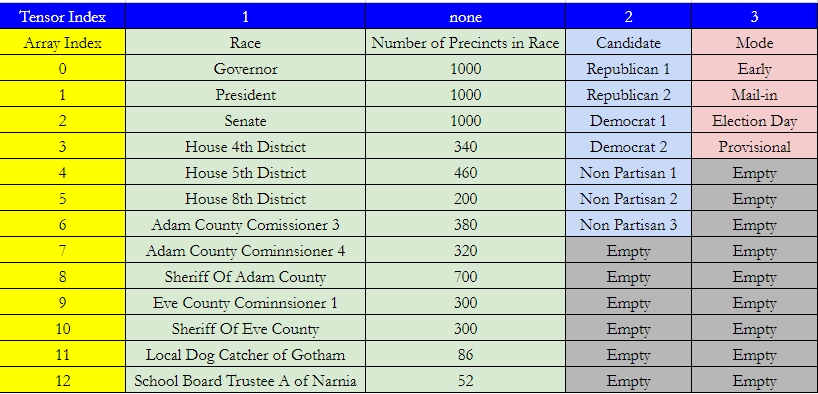
\includegraphics[width=400pt]{Precinct Library Card.png}
\end{center}
\end{figure}
\newpage
\begin{definition}{Precinct Candidate Card}\\
For each race, the name of each candidate pertaining to each race's candidate index is to be displayed as follows. This is to ensure that all data analysts, regardless of the software used, will return the same tabulation result from any call function upon the Tabulation Tensor.
\end{definition}

The below figure flushes out all six candidate indices for each race, even though no race utilizes all indices simultaneously. This to ensure that cell volume of the Tabulation Array is equal to $\prod_{k=0}^{k=3} \beta_{k}$, which is why dynamic arrays are forbidden. Thus the Tabulation Array is a rectangular tesseract, comprised mostly of $\emptyset$ cell values, again, this is to ensure ease of replication.

A sample Tabulation Array has been provided by the following link:
\url{https://docs.google.com/spreadsheets/d/1n4BG-gfKxoFnP_gisKYtzkhtrUerYq2cj4cdeGkff3g/edit?usp=sharing}

\begin{figure}[bp!]
\begin{center}
\caption{Precinct Candidate Card}
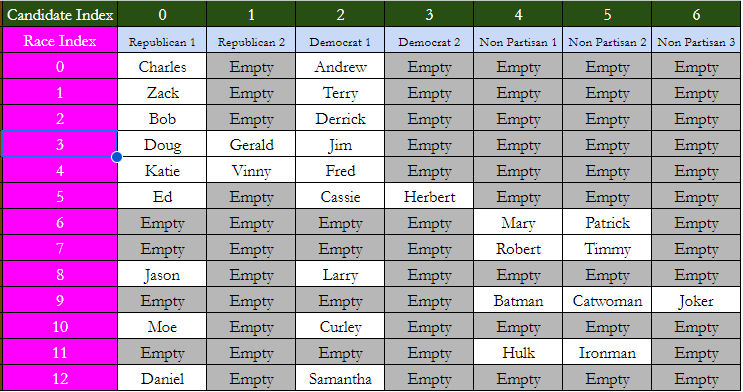
\includegraphics[width=400pt]{Candidate Card.png}
\end{center}
\end{figure}
\newpage
\subsection{Counting Group; S,T,U,V and Quantile Arrays; Data Set Definitions 2}
\begin{definition}{Local Counting Groups}\\
For any particular race, let each distinct pairing of a candidate and a mode be a Local Counting Group, such that the total number of distinct counting groups is equal to $\beta_{4}=\beta_{2}\beta_{3}$ (for instance, if there's three candidates and three ways of voting, then there's nine counting groups). Let \textbf{E} be a particular counting group for all precincts involved in a particular race, and let \textbf{F} be the set of all counting groups for all precincts involved in a particular race.\\

A Local Counting Group, \textbf{E}, does not contain any null entries. It is an isolated subset of non-empty tabulations for a particular race from the Tabulation Array. The Set of All Counting Groups, \textbf{F}, excludes any precincts that are not universally shared amongst all counting groups.

\textcolor{red}{If you only intend to read this article, you can skip the remainder of this definition}. 

If you are intending to write your code (in whatever software you choose) to analyze elections (or replicate my results), the rigorous definitions of the Local Counting Groups and the Set of All Counting Groups are as follows (which should be sufficient to guide your coding):

Let the set of all precinct indices be \textbf{W}, then:\\
For any particular race, $r$, and for any specified $c,d$ pairing such that:
$$\bigcup_{w=0}^{w=\beta_{0}-1}A_{w,r,c,d}\neq\emptyset$$

Then let $D_{1,0}=\bigcup_{w=0}^{w=\beta_{0}-1}A_{w,r,c,d}$ and let $D_{2,0}$ be the subset of $D_{1,0}$ that contains all empty elements of $D_{1,0}$, then \textbf{E} = $(D_{1,0}-D_{2,0})$ and let $W_{0}$ be the set of all precinct principal indices for each element in \textbf{E}, and let the number of indices of \textbf{E} be equal to $\Gamma_{0}$.

For each distinct $c,d$ pairing that permits $\bigcup_{w=0}^{w=\beta_{0}-1}A_{w,r,c,d}\neq\emptyset$, let each $c$ be placed into the set $C_{2}$ and let each $d$ be placed into the set $D_{2}$, and let the number of distinct candidate and mode indices in $C_{2}$ and $D_{2}$ be $\Upsilon_{1}$ and $\Upsilon_{2}$ respectively, and let $\Upsilon_{1} \Upsilon_{2}=\Upsilon_{3}$, and let the first element of $C_{2}$ and $D_{2}$ be the zeroth element, and let an element of either $C_{2}$ or $D_{2}$ be denoted as $c_{2,i}$ or $d_{2,j}$ respectively.

Then $\forall i, 0 \le i \le \Upsilon_{1}$ and $\forall j, 0 \le j \le \Upsilon_{2}$, let $k=(\Upsilon_{2}i+j)$.
\newpage
Then let $D_{1,k}=\bigcup_{w=0}^{w=\beta_{0}-1}A_{w,r,(c_{2,i}),(d_{2,j})}$ and let $D_{2,k}$ be the subset of $D_{1,k}$ that contains all empty elements of $D_{1,k}$, then $E_{k}=(D_{1,k}-D_{2,k})$ and let $W_{k}$ be the set of all precinct principal indices for each element in $E_{k}$, and let the number of indices of $E_{k}$ be equal to $\Gamma_{k}$. Then let:

$$W_{F} = \bigcap_{k=0}^{k=\Upsilon_{3}-1}W_{k}$$

And let an element of $W_{F}$ be denoted as $w_{f,b}$, denoting the ``$b^{th}$" element of the intersection of all $W_{k}$, and let the first element of $W_{F}$ be the zeroth element ($W_{F}$ is sorted from least to greatest).

Finally let the number of elements in $W_{F}$ be equal to $\beta_{5}$, then the set of all counting groups, \textbf{F}, for a particular race, is defined as:
$$F=\bigcup_{b=0}^{b=(\beta_{5}-1)}(\bigcup_{i=0}^{i=(\Upsilon_{1}-1)}(\bigcup_{j=0}^{j=(\Upsilon_{2}-1)}A_{(w_{f,b}),(r),(c_{2,i}),(d_{2,j})})))$$

We leave \textbf{F} in its Array Form for analysis (the number of columns is equal to $\Upsilon_{3}$).
\end{definition}

Visit the sheet titled ``Set of Counting Groups," in the following link: \url{https://docs.google.com/spreadsheets/d/1n4BG-gfKxoFnP_gisKYtzkhtrUerYq2cj4cdeGkff3g/edit?usp=sharing}

You will see \textcolor{red}{in cell H1} there is an operator that requests the Race Number. When a valid race number is entered it immediately produces \textbf{F}.  Whichever software and coding you use (such as MATLAB or Python), it must be capable of producing \textbf{F} with no errors or ambiguities as seen in the spreadsheet example.

When you visit the spreadsheet link, you can go to ``File" and then ``Make a Copy" to learn and experiment with the optimal spreadsheet code that I wrote to accomplish this in Excel. 

The reason I personally do everything in Excel is because it can be replicated by members of the general public (it does not require coding knowledge specialized for a particular piece of software or platform). It can also be examined, cell by cell, to ensure integrity in the coding.

No calculation can be hidden in a spreadsheet, which is why it the best tool in a Court of Law (whereas applications like MATLAB and Python put you at the programmer's mercy).
\newpage
\begin{definition}{Real Number S,T,U,V Array, the Analyzed Precincts and the Culled Precincts}\\
For any particular race, let \textbf{S,T,U} and \textbf{V} be any four pairwise disjoint non-empty subsets of the Set of all Counting Groups, \textbf{F}, where each element of \textbf{S,T,U} and \textbf{V} is equal to the sum of all ballots cast for all counting groups in each subset.

No counting group can be included multiple times (disjoint subsets), nor can any subset, \textbf{S,T,U} or \textbf{V}, be empty. Thus, if an election only has one form of voting, then no analysis can be done if there's only two candidates.

Now let $P_{2}$ be the subset of \textbf{P} that contains all of the precincts in \textbf{F} for some \textbf{S,T,U} and \textbf{V} denomination of some particular race and let $p_{2,b}$ be the $b^{th}$ element of $P_{2}$ (remember that the number of precincts in $P_{2}$ is equal to $\beta_{5}$).

Then, for some arbitrary cull number, $\Psi$, that if either:\\
$s_{b}+t_{b}<\Psi$ ; or,\\
$s_{b}+u_{b}<\Psi$ ; or,\\
$s_{b}+v_{b}<\Psi$ ; or,\\
$t_{b}+u_{b}<\Psi$ ; or,\\
$t_{b}+v_{b}<\Psi$ ; or,\\
$s_{u}+u_{v}<\Psi$

Then let that precinct, $p_{2,b}$, be placed in the set $P_{3}$ and let the number of precincts in $P_{3}$ be equal to $\beta_{6}$, then let \textbf{Q}=$(P_{2}-P_{3})$ be the \textbf{Set of Analyzed Precincts} such that the number of precincts in \textbf{Q} is equal to $\beta_{7}=(\beta_{5}-\beta_{6})$. Also, let $P_{3}$ be named the \textbf{Set of Culled Precincts} and let the set $W_{Q}$ be the set of principal precinct indices for all precincts in \textbf{Q}, sorted from least to greatest in order to preserve the original alphanumeric ordering from the Tabulation Array.
\end{definition}

This is called a ``Real Number" STUV Array, because when we're only analyzing a single race, we use real numbers.

When we analyze two races simultaneously, we need Complex Numbers (The Twenty Laws and Forty Isometries hold for Complex Numbers). When we analyze Four Races at a time, we need the Quaternions (The Twenty Laws and Forty Isometries hold for the Quaternions, assuming one minds left and right handed multiplication and division).

Go to the sheet ``Set Counting Groups" in \url{https://docs.google.com/spreadsheets/d/1n4BG-gfKxoFnP_gisKYtzkhtrUerYq2cj4cdeGkff3g/edit?usp=sharing}.

The STUV assignments set as binary column vectors in cells B2 to E29. If the value is 1, then that counting group is included within the respective subset. We then multiply each $b^{th}$ row vector of the \textbf{F} Array by the S,T,U and V binary column vectors to yield $s_{b}, t_{b}, u_{b}$ and $v_{b}$ in each precinct.
\newpage
The arbitrary cull number of $\Psi$ should be set to 50 for low turnout general elections, 100 for high turnout general elections and 30 for low turnout primary elections.

The cull number ensures a decimal resolution of $\frac{1}{\Psi}$ for the denominators of $x,y,g,h,m$ and $n$ (that is, for the quadrant pairing percentages of North vs South, West vs East and Diagonal vs Diagonal); whilst ensuring a decimal resolution of $\frac{1}{2\Psi}$ for the denominators of $\Omega,\alpha,\lambda$. 

A culling is performed to avoid false negatives for election fraud, since an election with 10 votes cast will have a residual error of 10\% in its aggregate percentages, such that a sizeable collection of precincts with low vote totals would adversely effect the $R^2$ values of any manifold regression of any three percentages (from the same Orientation, such as North vs South), allowing a rigged election to escape detection. 

Any additional precincts that are culled for other reasons (for instance, in Nevada, the mean value of $\lambda$ was 0.635 with a small standard deviation, but there were three precincts that were more than five standard deviations above/below the mean that were removed from the analyzed set), must be specified in writing.

If you do wish to cull any precincts from the Analyzed Set, then when any regression of the data is performed over the precincts, the RSS and TSS (Residual Sum of Squares and Total Sum of Squares) for each $b^{th}$ precinct must be weighted by the formula $\frac{s_{b}+t_{b}+u_{b}+v_{b}}{S+T+U+V}$, where the denominator is sum all of S,T,U,V ballot categories for all precincts in the data set. \textcolor{red}{No other form of weighting may be used. This form of weighting only takes into account the number of ballots cast at the precinct compared to that of the entire dataset}.

The advantage of a cull number is that it does not introduce any  bias into the results, the precincts are simply culled by an arbitrary number of ballots cast. This is why \textbf{I personally prefer} using a Cull Number rather than weight based upon ballots cast.

Whereas using the above weighting function will alter the $R^2$ in manner that reflects the precincts with the largest vote totals (that is, the final quartile of the precinct set carries the most weight)--- yet once a decimal resolution of 1\% is reached in the denominator (a precinct with 100 total votes cast), the $R^2$ of the regression should no longer be adversely affected by the quantization of the denominator.

Election reports from Caucus events, such as in Iowa, that have four or more candidates can be analyzed, which is important in the age of ``Remote Satellite Caucuses," which is an overt effort to remove the physical in-person and easily verified headcount of a traditional caucus event inside of a high-school gymnasium (Bernie Sanders primaries and caucuses in 2016 and 2020 are definitely interesting in the context of this publication!).

The last definition illustrates why universal mail-in voting (with no alternate option, like in Oregon), because we can no longer analyze and contrast the behaviors of different subsets of the electorate for suspicious activity, as we'll usually be left with only two significant candidates with one mode of unsupervised voting, yielding only two distinct unsupervised counting groups.

This is also why Ranked-Choice Voting is so dangerous, because we can no longer form disjoint subsets, as the reported numbers for each candidate are derived from a conflated group of voters (thus, the numbers reported are not disjoint).

Finally, this is why the heavy reduction of geographical precincts (like in Illinois) is dangerous, because suspicious activity can be smoothed out over a smaller group of precincts with large population sizes, with no way to recover local trends.

Sadly, we have politicians that are actively trying to pursue universal mail-in ranked-choice voting all tabulated at one central location...do you see the problem? 

They aren't doing this for ``convenience" or ``accessibility" or ``fairness." They are doing it because the voting software companies are instructing them to. The voting software companies do not want people like you or me to analyze the results of their product.
\newpage
\subsection{Ordinal, Percentage and Quantile Functions of an STUV Array}
\begin{definition}{The Precinct Ordinal Function, The Percentage Array}\\
Given a set of analyzed precincts, \textbf{Q}, let the precincts in \textbf{Q} be sorted from least to greatest alphanumerically (this sorting should be automatic since $W_{F}$ is sorted numerically, which is derived from \textbf{W}, which itself preserves the alphanumeric ordering of all precincts in \textbf{Q}), such that $q_{b}$ is the $b^{th}$ precinct in the list (remember that $\beta_{7}$ is the total number of precincts in \textbf{Q}) and let the first precinct in the list be the \textcolor{red}{FIRST} element of \textbf{Q}. That is, we start with the Ordinal 1, instead of zero, for the principal subset index.

Also, let $b$ be known as the \textbf{Principal Subset Index}.

Then for each precinct, $q_{b}$ , in \textbf{Q}, let:

$x_{b}=\frac{s_{b}}{s_{b}+t_{b}}$

$y_{b}=\frac{u_{b}}{u_{b}+v_{b}}$

$g_{b}=\frac{s_{b}}{s_{b}+v_{b}}$

$h_{b}=\frac{u_{b}}{u_{b}+t_{b}}$

$m_{b}=\frac{s_{b}}{s_{b}+u_{b}}$

$n_{b}=\frac{t_{b}}{t_{b}+v_{b}}$

$\Omega_{b}=\frac{s_{b}+t_{b}}{(s_{b}+t_{b})+(u_{b}+v_{b})}$

$\alpha_{b}=\frac{s_{b}+u_{b}}{(s_{b}+u_{b})+(t_{b}+v_{b})}$

$\lambda_{b}=\frac{s_{b}+v_{b}}{(s_{b}+v_{b})+(u_{b}+t_{b})}$

Let the Percentage Arrays, \textbf{X,Y,G,H,M,N,O,A,L} be the respective sequences of $x_{b}, y_{b}, g_{b}, h_{b}, m_{b}, n_{b}, \Omega_{b}, \alpha_{b}$ and $\lambda_{b}$ for the precincts in \textbf{Q}, and let the array indices of the above be numbered from 1 to 9 (respectively).

Now let the set $W_{Q}$be the zeroth index of this array, so that there also exists a map back to the Tabulation Array.

Then let an element of Percentage Array be notated as $Z_{b,z,0}$, denoting the $b^{th}$ precinct in the $z^{th}$ array, with ``0" denoting that it is the Percentage Array.

Then let the function $\omega_{0}(q_{b})$ return the ordinal of the alphanumeric ranking of precinct $q_{b}$, such that $\omega_0{q_{b}}=b$.
\newpage
Finally, let $\omega_{z}(q_{b})$ return the ordinal of the numeric ranking of precinct $q_{b}$'s percentage in the respective array index (for instance, $\omega_{3}(q_{b})$ would return the ordinal of the numeric ranking the precinct's $g_{b}$ percentage within the entirety of the \textbf{G} Percentage Array, since 3 is the array index of \textbf{G}), such that any ties in the numeric ranking are broken by $\omega_{0}(q_{b})$. 

That is, ties are broken between precincts with the same rational number percentages (since votes are integers) by their alphanumeric ranking, which is unique. This is to ensure that there exists a pairwise bijection between the all of the ordinal rankings of all the Percentage Arrays.
\end{definition}

\begin{definition}{The Quantile Array and The Analysis Tensor}\\
Let the Quantile Arrays $Q_{X},Q_{Y},Q_{G},Q_{H},Q_{M},Q_{N},Q_{O},Q_{A},Q_{L}$ be the quantiles of each Percentage Array, and let their array indices be numbered from 1 to 9 respectively, such that each element of the respective arrays are equal to $\frac{\omega_{z}(q_{b})}{\beta_{7}}$ ,where $z$ is the array index of the Quantile Array in question, which corresponds directly the array indices of 1 through 9 of the Percentage Arrays).

Let the Array \textbf{B} be the zeroth index of this array, so that there exists an internal map with the Analysis Tensor.

Then let an element of the Quantile Array be notated as $Z_{b,z,1}$, denoting the $b^{th}$ precinct in the $z^{th}$ array, with ``1" denoting that it is in the Quantile Array.

Finally, let $Z_{b,z,a}$ be \textbf{The Analysis Tensor}, denoting the  $b^{th}$ precinct in the $z^{th}$ array in the $a^{th}$ array layer. 
\end{definition}

We shall be adding additional layers to this array as the definitions progress.

Go to the sheet titled ``PercentQuantile Arrays" in \url{https://docs.google.com/spreadsheets/d/1n4BG-gfKxoFnP_gisKYtzkhtrUerYq2cj4cdeGkff3g/edit?usp=sharing}.

In Columns M to U you see the Percentage Array. In Columns V to AD you see the Quantile Array.

Also, as an added note, since you must enter the STUV denominations manually (via the binary column vectors), you must ensure that your chosen STUV denomination is in fact---Disjoint.

On the sheet ``Set of Counting Groups" in cell F30, you will see the confirmation code that the chosen STUV denomination is disjoint.
\newpage
\begin{definition}{The Mean and Standard Deviation Array}\\
For a given set of Analyzed Precincts:\\
Let $\mu_{1}, \mu_{2}, \mu_{3}, \mu_{4}, \mu_{5}, \mu_{6}, \mu_{7}, \mu_{8}, \mu_{9}$ be the mean value $x_{b}, y_{b}, g_{b}, h_{b}, m_{b}, n_{b}, \Omega_{b}, \alpha_{b}, \lambda_{b}$ across the precincts (respectively), which can also be written as (for ease of human interpretation) as:\\
$\mu_{X}, \mu_{Y}, \mu_{G}, \mu_{H}, \mu_{M}, \mu_{N}, \mu_{O}, \mu_{A}, \mu_{L}$

Let $\sigma_{1}, \sigma_{2}, \sigma_{3}, \sigma_{4}, \sigma_{5}, \sigma_{6}, \sigma_{7}, \sigma_{8}, \sigma_{9}$ be the standard deviation of the sample variance for $x_{b}, y_{b}, g_{b}, h_{b}, m_{b}, n_{b}, \Omega_{b}, \alpha_{b}, \lambda_{b}$ across the precincts (respectively), which can also be written as (for ease of human interpretation) as:\\
$\sigma_{X}, \sigma_{Y}, \sigma_{G}, \sigma_{H}, \sigma_{M}, \sigma_{N}, \sigma_{O}, \sigma_{A}, \sigma_{L}$

$\mu_{1}=\mu_{X}=\sum_{b=1}^{b=\beta_{7}}\frac{Z_{b,1,0}}{\beta_{7}}$; $\sigma_{1}=\sigma_{X}=\sqrt{\frac{\sum_{b=1}^{b=\beta_{7}}(Z_{b,1,0}-\mu_{1})^2}{\beta_{7}}}=\sqrt{\frac{\sum_{b=1}^{b=\beta_{7}}(x_{b}-\mu_{X})^2}{\beta_{7}}}$

$\mu_{2}=\mu_{Y}=\sum_{b=1}^{b=\beta_{7}}\frac{Z_{b,2,0}}{\beta_{7}}$; $\sigma_{2}=\sigma_{Y}=\sqrt{\frac{\sum_{b=1}^{b=\beta_{7}}(Z_{b,2,0}-\mu_{2})^2}{\beta_{7}}}=\sqrt{\frac{\sum_{b=1}^{b=\beta_{7}}(y_{b}-\mu_{Y})^2}{\beta_{7}}}$

$\mu_{3}=\mu_{G}=\sum_{b=1}^{b=\beta_{7}}\frac{Z_{b,3,0}}{\beta_{7}}$; $\sigma_{3}=\sigma_{G}=\sqrt{\frac{\sum_{b=1}^{b=\beta_{7}}(Z_{b,3,0}-\mu_{3})^2}{\beta_{7}}}=\sqrt{\frac{\sum_{b=1}^{b=\beta_{7}}(g_{b}-\mu_{G})^2}{\beta_{7}}}$

$\mu_{4}=\mu_{H}=\sum_{b=1}^{b=\beta_{7}}\frac{Z_{b,4,0}}{\beta_{7}}$; $\sigma_{4}=\sigma_{H}=\sqrt{\frac{\sum_{b=1}^{b=\beta_{7}}(Z_{b,4,0}-\mu_{4})^2}{\beta_{7}}}=\sqrt{\frac{\sum_{b=1}^{b=\beta_{7}}(h_{b}-\mu_{H})^2}{\beta_{7}}}$

$\mu_{5}=\mu_{M}=\sum_{b=1}^{b=\beta_{7}}\frac{Z_{b,5,0}}{\beta_{7}}$; $\sigma_{5}=\sigma_{M}=\sqrt{\frac{\sum_{b=1}^{b=\beta_{7}}(Z_{b,5,0}-\mu_{5})^2}{\beta_{7}}}=\sqrt{\frac{\sum_{b=1}^{b=\beta_{7}}(m_{b}-\mu_{M})^2}{\beta_{7}}}$

$\mu_{6}=\mu_{N}=\sum_{b=1}^{b=\beta_{7}}\frac{Z_{b,6,0}}{\beta_{7}}$; $\sigma_{6}=\sigma_{N}=\sqrt{\frac{\sum_{b=1}^{b=\beta_{7}}(Z_{b,6,0}-\mu_{6})^2}{\beta_{7}}}=\sqrt{\frac{\sum_{b=1}^{b=\beta_{7}}(n_{b}-\mu_{N})^2}{\beta_{7}}}$

$\mu_{7}=\mu_{O}=\sum_{b=1}^{b=\beta_{7}}\frac{Z_{b,7,0}}{\beta_{7}}$; $\sigma_{7}=\sigma_{O}=\sqrt{\frac{\sum_{b=1}^{b=\beta_{7}}(Z_{b,7,0}-\mu_{7})^2}{\beta_{7}}}=\sqrt{\frac{\sum_{b=1}^{b=\beta_{7}}(\Omega_{b}-\mu_{O})^2}{\beta_{7}}}$

$\mu_{8}=\mu_{A}=\sum_{b=1}^{b=\beta_{7}}\frac{Z_{b,8,0}}{\beta_{7}}$; $\sigma_{8}=\sigma_{A}=\sqrt{\frac{\sum_{b=1}^{b=\beta_{7}}(Z_{b,8,0}-\mu_{8})^2}{\beta_{7}}}=\sqrt{\frac{\sum_{b=1}^{b=\beta_{8}}(\alpha_{b}-\mu_{A})^2}{\beta_{7}}}$

$\mu_{9}=\mu_{L}=\sum_{b=1}^{b=\beta_{7}}\frac{Z_{b,9,0}}{\beta_{7}}$; $\sigma_{9}=\sigma_{L}=\sqrt{\frac{\sum_{b=1}^{b=\beta_{7}}(Z_{b,9,0}-\mu_{9})^2}{\beta_{7}}}=\sqrt{\frac{\sum_{b=1}^{b=\beta_{7}}(\lambda_{b}-\mu_{L})^2}{\beta_{7}}}$
\end{definition}
\newpage
\subsection{Convergence, Constraint and Irrelevance Lemmas}
\textcolor{red}{Note: The final line in the below table is does not contain typos. As $\Omega_{2}$ goes to zero, both alpha and lambda approach $x_{1}$.}

\begin{lemma}{The Aggregate Convergence Lemma}
\end{lemma}
\SetTblrInner{rowsep=5pt,colsep=2pt}
\begin{tblr}{|l|l|l|}
\hline
North vs South & West vs East & Diagonal vs Diagonal\\
\hline
$\lim_{\Omega_{1}\to 0}; x_{1}\Omega_{1}+\Omega_{2}y_{1}=y_{1}$ & $\lim_{\lambda_{1}\to 0}; g_{1}\lambda_{1}+\lambda_{2}h_{1}=h_{1}$ & $\lim_{\alpha_{1}\to 0}; m_{1}\alpha_{1}+\alpha_{2}n_{1}=n_{1}$\\
\hline
$\lim_{\Omega_{1}\to 0}; x_{2}\Omega_{1}+\Omega_{2}y_{2}=y_{2}$ & $\lim_{\lambda_{1}\to 0}; g_{2}\lambda_{1}+\lambda_{2}h_{2}=h_{2}$ & $\lim_{\alpha_{1}\to 0}; m_{2}\alpha_{1}+\alpha_{2}n_{2}=n_{2}$\\
\hline
$\lim_{\Omega_{1}\to 0}; \alpha_{1}=y_{1}$ & $\lim_{\lambda_{1}\to 0}; \alpha_{1}=h_{1}$ & $\lim_{\alpha_{1}\to 0}; \Omega_{1}=n_{1}$\\
\hline
$\lim_{\Omega_{1}\to 0}; \lambda_{1}=y_{2}$ & $\lim_{\lambda_{1}\to 0}; \Omega_{1}=h_{2}$ & $\lim_{\alpha_{1}\to 0}; \lambda_{1}=n_{2}$\\
\hline
$\lim_{\Omega_{2}\to 0}; x_{1}\Omega_{1}+\Omega_{2}y_{1}=x_{1}$ & $\lim_{\lambda_{2}\to 0}; g_{1}\lambda_{1}+\lambda_{2}h_{1}=g_{1}$ & $\lim_{\alpha_{2}\to 0}; m_{1}\alpha_{1}+\alpha_{2}n_{1}=m_{1}$\\
\hline
$\lim_{\Omega_{2}\to 0}; x_{2}\Omega_{1}+\Omega_{2}y_{2}=x_{2}$ & $\lim_{\lambda_{2}\to 0}; g_{2}\lambda_{1}+\lambda_{2}h_{2}=g_{2}$ & $\lim_{\alpha_{2}\to 0}; m_{2}\alpha_{1}+\alpha_{2}n_{2}=m_{2}$\\
\hline
$\lim_{\Omega_{2}\to 0}; \alpha_{1}=x_{1}$ & $\lim_{\lambda_{2}\to 0}; \alpha_{1}=g_{1}$ & $\lim_{\alpha_{2}\to 0}; \Omega_{1}=m_{1}$\\
\hline
$\lim_{\Omega_{2}\to 0}; \lambda_{1}=x_{1}$ & $\lim_{\lambda_{2}\to 0}; \Omega_{1}=g_{1}$ & $\lim_{\alpha_{2}\to 0}; \lambda_{1}=m_{1}$\\
\hline
\end{tblr}

\begin{corollary} Data Set $R^2$ Convergences\\
As the mean value of $\Omega_{1}$ approaches zero across a data set, the $R^2$ of the regressions of following regression approach 1.0:\\
$y_{1}$ or $y_{2}$ in terms of $\alpha_{1}$ or $\alpha_{2}$; or,\\
$\alpha_{1}$ or $\alpha_{2}$ in terms of $y_{1}$ or $y_{2}$; or,\\
$y_{1}$ or $y_{2}$ in terms of $\lambda_{1}$ or $\lambda_{2}$; or,\\
$\lambda_{1}$ or $\lambda_{2}$ in terms of $y_{1}$ or $y_{2}$

As the mean value of $\Omega_{2}$ approaches zero across a data set, the $R^2$ of the regressions of following regression approach 1.0:\\
$x_{1}$ or $x_{2}$ in terms of $\alpha_{1}$ or $\alpha_{2}$; or,\\
$\alpha_{1}$ or $\alpha_{2}$ in terms of $x_{1}$ or $x_{2}$; or,\\
$x_{1}$ or $x_{2}$ in terms of $\lambda_{1}$ or $\lambda_{2}$; or,\\
$\lambda_{1}$ or $\lambda_{2}$ in terms of $x_{1}$ or $x_{2}$

As the mean value of $\lambda_{1}$ approaches zero across a data set, the $R^2$ of the regressions of following regression approach 1.0:\\
$h_{1}$ or $h_{2}$ in terms of $\alpha_{1}$ or $\alpha_{2}$; or,\\
$\alpha_{1}$ or $\alpha_{2}$ in terms of $h_{1}$ or $h_{2}$; or,\\
$h_{1}$ or $h_{2}$ in terms of $\Omega_{1}$ or $\Omega_{2}$; or,\\
$\Omega_{1}$ or $\Omega_{2}$ in terms of $h_{1}$ or $h_{2}$
\newpage
As the mean value of $\lambda_{2}$ approaches zero across a data set, the $R^2$ of the regressions of following regression approach 1.0:\\
$g_{1}$ or $g_{2}$ in terms of $\alpha_{1}$ or $\alpha_{2}$; or,\\
$\alpha_{1}$ or $\alpha_{2}$ in terms of $g_{1}$ or $g_{2}$; or,\\
$g_{1}$ or $g_{2}$ in terms of $\Omega_{1}$ or $\Omega_{2}$; or,\\
$\Omega_{1}$ or $\Omega_{2}$ in terms of $g_{1}$ or $g_{2}$

As the mean value of $\alpha_{1}$ approaches zero across a data set, the $R^2$ of the regressions of following regression approach 1.0:\\
$n_{1}$ or $n_{2}$ in terms of $\Omega_{1}$ or $\Omega_{2}$; or,\\
$\Omega_{1}$ or $\Omega_{2}$ in terms of $n_{1}$ or $n_{2}$; or,\\
$n_{1}$ or $n_{2}$ in terms of $\lambda_{1}$ or $\lambda_{2}$; or,\\
$\lambda_{1}$ or $\lambda_{2}$ in terms of $n_{1}$ or $n_{2}$

As the mean value of $\alpha_{2}$ approaches zero across a data set, the $R^2$ of the regressions of following regression approach 1.0:\\
$m_{1}$ or $m_{2}$ in terms of $\Omega_{1}$ or $\Omega_{2}$; or,\\
$\Omega_{1}$ or $\Omega_{2}$ in terms of $m_{1}$ or $m_{2}$; or,\\
$m_{1}$ or $m_{2}$ in terms of $\lambda_{1}$ or $\lambda_{2}$; or,\\
$\lambda_{1}$ or $\lambda_{2}$ in terms of $m_{1}$ or $m_{2}$
\end{corollary}

For this reason, one must exercise great caution when making claim about manifold appearing in an election with a very high (or low) mean value of any of the three aggregates, $\alpha, \Omega, \lambda$.

In order to deal with such situations, no less than 10,000 Quantile Simulations of the Election must be performed, in order to ascertain the expected $R^2$ of such manifolds for a statistically identical election.

\begin{corollary} The Irrelevance Theorem\\
As the mean value of $\Omega_{1}$ approaches zero across a data set, the $R^2$ of the regressions of following regression approach zero:\\
$x_{1}$ (or $x_{2}$) in terms of $\alpha_{1}$ (or $\alpha_{2}$) and $y_{1}$ (or $y_{2}$); or,\\
$x_{1}$ (or $x_{2}$) in terms of $\lambda_{1}$ (or $\lambda_{2}$) and $y_{1}$ (or $y_{2}$); or,\\

As the mean value of $\Omega_{2}$ approaches zero across a data set, the $R^2$ of the regressions of following regression approach zero:\\
$y_{1}$ (or $y_{2}$) in terms of $\alpha_{1}$ (or $\alpha_{2}$) and $x_{1}$ (or $x_{2}$); or,\\
$y_{1}$ (or $y_{2}$) in terms of $\lambda_{1}$ (or $\lambda_{2}$) and $x_{1}$ (or $x_{2}$); or,\\

As the mean value of $\lambda_{1}$ approaches zero across a data set, the $R^2$ of the regressions of following regression approach zero:\\
$g_{1}$ (or $g_{2}$) in terms of $\alpha_{1}$ (or $\alpha_{2}$) and $h_{1}$ (or $h_{2}$); or,\\
$g_{1}$ (or $g_{2}$) in terms of $\Omega_{1}$ (or $\Omega_{2}$) and $h_{1}$ (or $h_{2}$); or,\\

As the mean value of $\lambda_{2}$ approaches zero across a data set, the $R^2$ of the regressions of following regression approach zero:\\
$h_{1}$ (or $h_{2}$) in terms of $\alpha_{1}$ (or $\alpha_{2}$) and $g_{1}$ (or $g_{2}$); or,\\
$h_{1}$ (or $h_{2}$) in terms of $\Omega_{1}$ (or $\Omega_{2}$) and $g_{1}$ (or $g_{2}$); or,\\

As the mean value of $\alpha_{1}$ approaches zero across a data set, the $R^2$ of the regressions of following regression approach zero:\\
$m_{1}$ (or $m_{2}$) in terms of $\Omega_{1}$ (or $\Omega_{2}$) and $n_{1}$ (or $n_{2}$); or,\\
$m_{1}$ (or $m_{2}$) in terms of $\lambda_{1}$ (or $\lambda_{2}$) and $n_{1}$ (or $n_{2}$); or,\\

As the mean value of $\alpha_{2}$ approaches zero across a data set, the $R^2$ of the regressions of following regression approach zero:\\
$n_{1}$ (or $n_{2}$) in terms of $\Omega_{1}$ (or $\Omega_{2}$) and $m_{1}$ (or $m_{2}$); or,\\
$n_{1}$ (or $n_{2}$) in terms of $\lambda_{1}$ (or $\lambda_{2}$) and $m_{1}$ (or $m_{2}$); or,\\
\end{corollary}

In other words, the as one portion of the total vote becomes irrelevant (for instance if the proportion of Election Day to Mail-in ballots was absurdly low, then the election day percentage at a precinct carries no effective weight on the aggregate and is pretty much irrelevant), the ability to predict the percentage of ballots cast in the irrelevant category becomes increasing difficult from the aggregate percentage and the percentage of ballots in the other category (that is, from the example in the prior set of parentheses, it would become nearly impossible to predict a candidate's election day percentage at a precinct from the candidate's aggregated and mail-in percentage when the mean value of $\Omega_{1}$, which is the percentage of ballots cast that are election day ballots, is close to 0\%).

Hence, it would be extraordinary unusual to be able to predict both $x_{1}$ from $\alpha$ and $y_{1}$, and, $y_{1}$ from $\alpha$ and $x_{1}$ with an $R^2$ in excess of 0.99 for both regression in a normal election possessing meaningful varation for $\Omega_{1}$.

Likewise, it would be extraordinary unusual to be able to predict both $g_{1}$ from $\alpha$ and $h_{1}$, and, $h_{1}$ from $\alpha$ and $g_{1}$ with an $R^2$ in excess of 0.99 for both regressions in a normal election possessing meaningful variation for $\lambda_{1}$; yet, in Atlanta, Georgia, we can in fact predict both with $\lambda_{1}$ having a standard deviation well in excess of 10\%, using an invertible quartic function.
\newpage
\begin{lemma}{Dual Aggregate Constraint Lemma}\\
Assuming that the data consists of positive integers (vote totals), then:\\

If both $\alpha_{1}$ (or $\alpha_{2}$) and $\lambda_{1}$ (or $\lambda_{2}$) are known, then the values of $x_{1}$ (or $x_{2}$) and $y_{1}$ (or $y_{2}$) are pigeonholed, such that both $x_{1}$ and $y_{1}$ can be predicted with near certainty.

If both $\alpha_{1}$ (or $\alpha_{2}$) and $\Omega_{1}$ (or $\Omega_{2}$) are known, then the values of $g_{1}$ (or $g_{2}$) and $h_{1}$ (or $h_{2}$) are pigeonholed, such that both $g_{1}$ and $h_{1}$ can be predicted with near certainty.

If both $\Omega_{1}$ (or $\Omega_{2}$) and $\lambda_{1}$ (or $\lambda_{2}$) are known, then the values of $m_{1}$ (or $m_{2}$) and $n_{1}$ (or $n_{2}$) are pigeonholed, such that both $m_{1}$ and $n_{1}$ can be predicted with near certainty.

As such, any regression of the above percentages, in respect to their corresponding pair of aggregate percentages (such as the regression of $x_{1}$ in terms of $alpha_{1}$ and $\lambda_{1}$), will result in $R^2$ values often exceeding 0.97.
\end{lemma}

For this reason, one must exercise great caution when making a claim about a double aggregate manifold in an election. 

This Lemma concerns the 3rd and 7th  Laws, and respective Isometries (numbers 23,43,27 and 47) and serves to protect the Defense against frivolous claims involving an alleged violation of these laws.

In order to deal with such situations, no less than 10,000 Quantile Simulations of the Election must be performed, in order to ascertain the expected $R^2$ of such manifolds for a statistically identical election.

\begin{lemma}{Single Aggregate Constraint Lemma}
Assuming that the data consists of positive integers (vote totals), then:

As $\Omega_{1}$ or $\Omega_{2}$ approach 0\%, knowledge of $g_{1}$ (or $g_{2}$); or, knowledge of $h_{1}$ (or $h_{2}$), pigeonholes the value of $h_{1}$ (or $h_{2}$); or, $g_{1}$ (or $g_{2}$) (respectively), such that any regression of any of these three percentages, from the remaining two percentages, will have an $R^2$ that approaches 1.

As $\Omega_{1}$ or $\Omega_{2}$ approach 0\%, knowledge of $m_{1}$ (or $m_{2}$); or, knowledge of $n_{1}$ (or $n_{2}$), pigeonholes the value of $n_{1}$ (or $n_{2}$); or, $m_{1}$ (or $m_{2}$) (respectively), such that any regression of any of these three percentages, from the remaining two percentages, will have an $R^2$ that approaches 1.
\newpage
As $\alpha_{1}$ or $\alpha_{2}$ approach 0\%, knowledge of $x_{1}$ (or $x_{2}$); or, knowledge of $y_{1}$ (or $y_{2}$), pigeonholes the value of $y_{1}$ (or $y_{2}$); or, $x_{1}$ (or $x_{2}$) (respectively), such that any regression of any of these three percentages, from the remaining two percentages, will have an $R^2$ that approaches 1.

As $\alpha_{1}$ or $\alpha_{2}$ approach 0\%, knowledge of $g_{1}$ (or $g_{2}$); or, knowledge of $h_{1}$ (or $h_{2}$), pigeonholes the value of $h_{1}$ (or $h_{2}$); or, $g_{1}$ (or $g_{2}$) (respectively), such that any regression of any of these three percentages, from the remaining two percentages, will have an $R^2$ that approaches 1.

As $\lambda_{1}$ or $\lambda_{2}$ approach 0\%, knowledge of $x_{1}$ (or $x_{2}$); or, knowledge of $y_{1}$ (or $y_{2}$), pigeonholes the value of $y_{1}$ (or $y_{2}$); or, $x_{1}$ (or $x_{2}$) (respectively), such that any regression of any of these three percentages, from the remaining two percentages, will have an $R^2$ that approaches 1.

As $\lambda_{1}$ or $\lambda_{2}$ approach 0\%, knowledge of $m_{1}$ (or $m_{2}$); or, knowledge of $n_{1}$ (or $n_{2}$), pigeonholes the value of $n_{1}$ (or $n_{2}$); or, $m_{1}$ (or $m_{2}$) (respectively), such that any regression of any of these three percentages, from the remaining two percentages, will have an $R^2$ that approaches 1.
\end{lemma}
\newpage
\begin{theorem}{Twixt Theorem}\\
The proportion of elements within the Union of the two disjoint sets \textbf{A} and \textbf{C}, that are contained with the superset \textbf{Z} that is the union of the four disjoint sets \textbf{A,B,C} and \textbf{D}, is always bounded between the proportion of elements in the Union of the two disjoint sets \textbf{X}, being the union of  \textbf{A} and \textbf{B}, and the proportion of the elements in the Union of the two disjoint sets \textbf{Y}, being the union of  \textbf{C} and \textbf{D}, thus it follows that:
$$\frac{a}{a+b}\le\frac{a+c}{a+b+c+d}\le\frac{c}{c+d}; or, \frac{c}{c+d}\le\frac{a+c}{a+b+c+d}\le\frac{a}{a+b}$$

Proof:
Given $\frac{a}{a+b}\le\frac{c}{c+d}$, then:

$\frac{a}{a+b}\le\frac{c}{c+d} \rightarrow ac+ad\le ac+bc \rightarrow ad\le bc$

$\frac{a}{a+b}\le\frac{a+c}{a+b+c+d} \rightarrow a^2+ab+ac+ad\le a^2+ab+ac+bc \rightarrow ad\le bc$

$\frac{a+c}{a+b+c+d}\le\frac{c}{c+d} \rightarrow ac+bc+c^2+cd\le ac+ad+c^2+cd \rightarrow ad\le bc$, therefore:

$x_{1} \le \alpha_{1} \le y_{1}; x_{1} \le \lambda_{1} \le y_{2}$

$g_{1} \le \alpha_{1} \le h_{1}; g_{1} \le \Omega_{1} \le h_{2}$

$m_{1} \le \Omega_{1} \le n_{1}; m_{1} \le \lambda_{1} \le n_{2}$
\end{theorem}

To put it simply, a candidate's aggregate percentage must be bounded between their Election Day and Mail-in Percentage at a precinct (and their West and East Side Percentages).
\begin{corollary}{North vs South Twixt Lemma}\\
As the average of the absolute value of the difference between $x_{1}$ and $y_{1}$ goes to zero across a dataset, the $R^2$ of a regression of either $x_{1}$ (or $x_{2}$), $y_{1}$ (or $y_{2}$), or $\alpha_{1}$ (or $\alpha_{2}$), from the remaining two percentages, goes to 1.

As the average of the absolute value of the difference between $x_{1}$ and $y_{2}$ goes to zero across a dataset, the $R^2$ of a regression of either $x_{1}$ (or $x_{2}$), $y_{2}$ (or $y_{1}$), or $\lambda_{1}$ (or $\lambda_{2}$), from the remaining two percentages, goes to 1.

More generally, as the average of the absolute value of the difference between either $x_{1}$ and $y_{1}$ (or $y_{2}$) ; or, $x_{2}$ and $y_{1}$ (or $y_{2})$ goes to 0 across a dataset, the values of $\alpha_{1},\alpha_{2}, \lambda_{1}$ and $\lambda_{2}$ are pigeonholed.
\end{corollary}
\begin{corollary}{West vs East Twixt Lemma}\\
As the average of the absolute value of the difference between $g_{1}$ and $h_{1}$ goes to zero across a dataset, the $R^2$ of a regression of either $g_{1}$ (or $g_{2}$), $h_{1}$ (or $h_{2}$), or $\alpha_{1}$ (or $\alpha_{2}$), from the remaining two percentages, goes to 1.

As the average of the absolute value of the difference between $g_{1}$ and $h_{2}$ goes to zero across a dataset, the $R^2$ of a regression of either $g_{1}$ (or $g_{2}$), $h_{2}$ (or $h_{1}$), or $\Omega_{1}$ (or $\Omega_{2}$), from the remaining two percentages, goes to 1.

More generally, as the average of the absolute value of the difference between either $g_{1}$ and $h_{1}$ (or $h_{2}$); or, $g_{2}$ and $h_{1}$ (or $h_{2}$) goes to 0 across a dataset, the values of $\alpha_{1},\alpha_{2}, \Omega_{1}$ and $\Omega_{2}$ are pigeonholed.
\end{corollary}
\begin{corollary}{Diagonal vs Diagonal Twixt Lemma}\\
As the average of the absolute value of the difference between $m_{1}$ and $n_{1}$ goes to zero across a dataset, the $R^2$ of a regression of either $m_{1}$ (or $m_{2}$), $n_{1}$ (or $n_{2}$), or $\Omega_{1}$ (or $\Omega_{2}$), from the remaining two percentages, goes to 1.

As the average of the absolute value of the difference between $m_{1}$ and $n_{2}$ goes to zero across a dataset, the $R^2$ of a regression of either $m_{1}$ (or $m_{2}$), $n_{2}$ (or $n_{1}$), or $\lambda_{1}$ (or $\lambda_{2}$), from the remaining two percentages, goes to 1.

More generally, as the average of the absolute value of the difference between either $m_{1}$ and $n_{1}$ (or $n_{2}$); or, $m_{2}$ and $n_{1}$ (or $n_{2}$) goes to 0 across a dataset, the values of $\Omega_{1},\Omega_{2}, \lambda_{1}$ and $\lambda_{2}$ are pigeonholed.
\end{corollary}

To paraphrase the above corollaries, if one plots the early and mail-in percentages of a candidate ($x_{1}$ and $y_{2}$), and they mostly (within 95\% of the data points) fall between the lines $y_{1}=x_{1}-0.1$ and $y_{1}=x_{1}+0.1$, then the regression of $\alpha_{1}$ from $x_{1}$ and $y_{1}$ (or any inversion of such a regression) will have a relatively high $R^2$ value.

The same idea applies for the West Side and East Side Percentages. If 95\% of the g,h coordinates fall between the lines $h_{1}=g_{1}-0.1$ and $h_{1}=g_{1}+0.1$, then we again expected a rather high $R^2$ value for the regression of $\alpha_{1}$ from $g_{1}$ and $h_{1}$.
\newpage
To know what the expected $R^2$ value is in a fair election under the same circumstances, one must perform a minimum of 10,000 quantile simulations replicating the local trajectory and residuals of $x_{1}, y_{1}$ and $\Omega_{1}$ over the quantiles of $x_{1}$, and then another 10,000 simulations of the same trajectories and residuals over the quantiles of $y_{1}$, and then perform the regression of $\alpha_{1}$ in terms of $x_{1}$ and $y_{1}$ and record the $R^2$ value of each simulation, then find the mean and standard deviation of the $R^2$ expectation and compare it against the actual election.

I have mentioned Quantile Simulations more than once---in Chapter 2 we will cover how one perform a Quantile Simulation of an election over the reals (single race), complex numbers (two races) and quaternions (four races).

In the below figure you see the map of $g_{1}$ and $h_{1}$ for the 2020 General Election of Clark and Washoe Counties for Trump and Biden. Although the majority of the data points fall within the ``Crest" (which is between the two outer red diagonal lines), because the standard deviation of $\lambda$ is effectively zero, the 3D scatter of $g_{1},h_{1}$ and $\alpha_{1}$ over the precincts would still form a flat plane with a very high $R^2$ value, regardless of where the $(g_{1},h_{1})$ coordinates were concentrated (which leads to the next corollary).
\begin{figure}[bp!]
\begin{center}
\caption{Trump vs Biden 2020 Nevada, Precincts in the Crest}
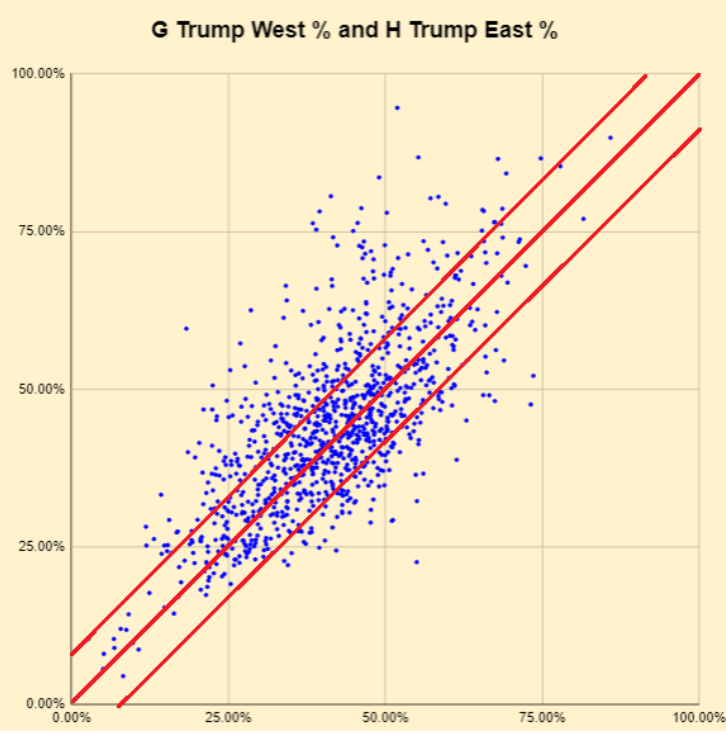
\includegraphics[width=250pt]{Twixt Lemma.png}
\end{center}
\end{figure}
\newpage
\begin{corollary}[The Expected 3D Boundaries of Alpha]
Assuming that the vote totals are positive integers, then:

Given $\mu_{7}=\mu_{O}$ and $\sigma_{7}=\sigma_{O}$, which is the mean and standard deviation of $\Omega_{1}$, and $\mu_{9}=\mu_{L}$ and $\sigma_{9}=\sigma_{L}$, which is the mean and standard deviation of $\lambda_{1}$, for some disjoint \textbf{S,T,U} and \textbf{V} denomination of the Analyzed Precincts, then from the Twixt Lemma we know that roughly 95\% of the $\alpha_{1,b}$ values are bounded between the two planes:

For the North vs South Orientation:
Case One:  For when $x_{1} \le y_{1}$, then:
$$(\mu_{7}-2\sigma_{7})x_{1,b} \le \alpha_{1} \le (1-\mu_{7}+2\sigma_{7})y_{1,b}$$
AND
$$(\mu_{7}+2\sigma_{7})x_{1,b} \le \alpha_{1} \le (1-\mu_{7}-2\sigma_{7})y_{1,b}$$

Case Two: For when $y_{1} < x_{1}$, then:
$$(1-\mu_{7}-2\sigma_{7})y_{1,b} < \alpha_{1} < (\mu_{7}+2\sigma_{7})x_{1,b}$$
AND
$$(1-\mu_{7}+2\sigma_{7})y_{1,b} < \alpha_{1} < (\mu_{7}-2\sigma_{7})x_{1,b}$$

Or more succinctly (for Case 1 and Case 2 respectively):\\
$\alpha_{1} \le +y_{1}+(2\sigma_{7}-\mu_{7})(x_{1}+y_{1})$ AND $\alpha_{1} \le +y_{1}-(2\sigma_{7}-\mu_{7})(x_{1}+y_{1})$\\
$\alpha_{1} \le -y_{1}+(\mu_{7}-2\sigma_{7})(x_{1}+y_{1})$ AND $\alpha_{1} \le -y_{1}+(\mu_{7}+2\sigma_{7})(x_{1}+y_{1})$

For the West vs East Orientation:
Case One:  For when $g_{1} \le h_{1}$, then:
$$(\mu_{9}-2\sigma_{9})g_{1,b} \le \alpha_{1} \le (1-\mu_{9}+2\sigma_{9})h_{1,b}$$
AND
$$(\mu_{9}+2\sigma_{9})g_{1,b} \le \alpha_{1} \le (1-\mu_{9}-2\sigma_{9})h_{1,b}$$

Case Two: For when $h_{1} < g_{1}$, then:
$$(1-\mu_{9}-2\sigma_{9})h_{1,b} < \alpha_{1} < (\mu_{9}+2\sigma_{9})g_{1,b}$$
AND
$$(1-\mu_{9}+2\sigma_{9})h_{1,b} < \alpha_{1} < (\mu_{9}-2\sigma_{9})g_{1,b}$$

Or more succinctly (for Case 1 and Case 2 respectively):\\
$\alpha_{1} \le +h_{1}+(2\sigma_{9}-\mu_{9})(g_{1}+h_{1})$ AND $\alpha_{1} \le +h_{1}-(2\sigma_{9}-\mu_{9})(g_{1}+h_{1})$\\
$\alpha_{1} \le -h_{1}+(\mu_{9}-2\sigma_{9})(g_{1}+h_{1})$ AND $\alpha_{1} \le -h_{1}+(\mu_{9}+2\sigma_{9})(g_{1}+h_{1})$
\end{corollary}
\newpage
Before we advance to the last two corollaries of the Twixt Lemma (which are trivial isomorphisms to the previous corollary), let's take a look at what this means.

The below link will bring you to a Simple (Non-Quantile) Simulator, which, given: 

(1) A set mean and standard deviation of the election day percentage, $x_{1}$, 
(2) A set mean and standard deviation of the difference from $x_{1}$ to $y_{1}$ (average difference between the election day and mail-in percentages across the precincts)
(3) A set mean and standard deviation for $\Omega_{1}$ (average percentage of ballots cast that are election day ballots)

Will then simulate 1000 precincts under the above three conditions, using the NORM.INV(RAND(), Mean, Sigma) Excel Function.

\url{https://docs.google.com/spreadsheets/d/1aWA9YcxXHFFV8zrV60BV_QJm-nt8qbSx9L3Rijh1b8Q/edit?usp=sharing}

After the precincts are simulated, it calculates the forced value of $\alpha_{1}$ via the Ninth Law. It then calculates the regression of $\alpha{1}$ in terms of $x_{1}$ and $y_{1}$ and the $R^2$ of the regression.  The simulation parameters for the mean and standard deviation of $\Omega_{1}$ are set in cells B3 and B4 (respectively).

Three simulations were setup for the mean and standard deviation of the election day and mail-in percentages in cells B7:B10 for the first simulation, cells B14:B17 for the second simulation and cells B21:B24 for the third simulation.

The $R^2$ return for each of the three simulations appear in cells B28:B30. Notice, that although the mean and standard of $\Omega_{1}$ is the same in all precincts, the expected $R^2$ values (after 100 trials) can be found in cells B32:B34 for each simulation, the standard deviation of the expected values (after 100 trials) can be found in cells B40:B42 and the Sigma Rating of the current simulation (the difference from the expected $R^2$ to the current $R^2$, divided by the standard deviation) can be found in cells B36:B38 for each of the three simulations.

Notice that although all three simulations have the mean and standard deviation for $\Omega_{1}$, that they have different mean and standard deviations for their expected $R^2$ values. This is due to the \textbf{Twixt Lemma}. As the absolute value of the mean difference between the election day and mail-in percentages ($x_{1}$ and $y_{1}$) increases, the expected $R^2$ decreases rapidly, but the standard deviation decreases slowly.

Overall, any election matching the conditions of any of those three simulated parameters, should produce an $R^2$ within five standard deviations of the mean expectation. 
\newpage
That being said, we do not use such simple parameters to run a simulation (the spreadsheet link was provided as a preliminary example of a simulation for the context of this subsection)---we use Quantile Simulations.

For now, observe (in Figure Ten below) that the $(x_{1},y_{1},\alpha_{1})$ coordinates of all three simulations are bounded between the same two planes (since they have the mean and standard deviation for $\Omega_{1}$), regardless of the mean and standard deviation of the election day percentage and the mean and standard deviation of the difference between the election day and mail-in percentages.

Here is direct link to the 3D Scatter Plot:\\
\url{https://plotly.com/~EKSolomon/100/}

This is why one must always observe the mean and standard deviations of $\Omega_{1}, \alpha_{1}$ and $\lambda_{1}$, and use their own common sense (prior to even running a quantile simulation) if the high $R^2$ of their manifold regression should be expected in a fair election under the same conditions.

Hence, there exists a potential ``Goldilocks Zone" for a \textbf{S,T,U,V} a denomination (Will County, Illinois being the ultimate example), where the mean values of \textcolor{red}{all} three aggregates bounded between 25\% and 75\%, and the mean difference (absolute) between the West and East Percentages is in excess of 25\%, yet an invertible and highly curved cubic manifold forms for $g_{1},h_{1},\alpha_{1}$ (unlike that flat plane of Clark County), with an $R^2$ well in excess of 0.99!

More likely than not (if the election was rigged), you will find that the manifold used to rig the election has an \textbf{S,T,U,V} denomination in the ``Goldilocks Zone," because such denominations are those that the Neural Network will find the most productive towards the manipulation the vote proportions.

\begin{figure}[bp!]
\begin{center}
\caption{X,Y,Alpha Coordinates of the Three Simulations}
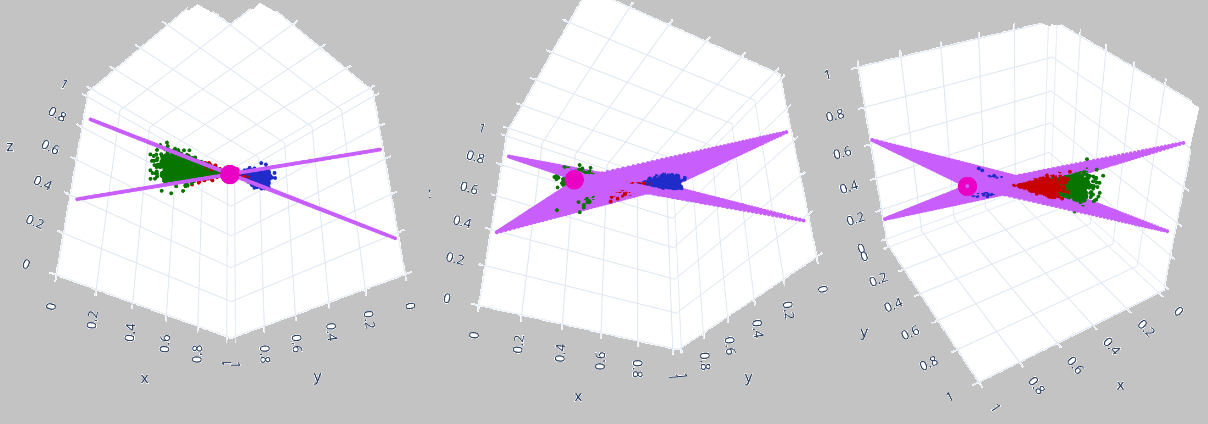
\includegraphics[width=400pt]{Twixtmebb.png}
\end{center}
\end{figure}
\newpage
Speaking of the ``Goldilocks Zone," although we do not have time to analyze Will County, Illinois in detail, I shall present the general results of that election.

For the 2022 General Election, in the Clerk's Race of Fritz vs Ferry, let:\\
$s_{b}$ be Fritz's Election Day Vote in each $b^th$ precinct.\\
$t_{b}$ be Ferry's Election Day Vote in each $b^th$ precinct.\\
$u_{b}$ be Frtiz's combined Early and Mail-in Vote in each $b^th$ precinct.\\
$v_{b}$ be Ferry's combined Early and Mail-in Vote in each $b^th$ precinct.

Let $g_{b,1}=\frac{s_{b}}{s_{b}+v{b}}$ be Ferry's West Side Ratio in each precinct.\\
Let $h_{b,1}=\frac{s_{b}}{u_{b}+t{b}}$ be Ferry's East Side Ratio in each precinct.\\
Let $\alpha_{b,1}=\frac{s_{b}+s_{b}}{s_{b}+t{b}+u_{b}+v{b}}$ be Ferry's Aggregate Percentage of all ballots cast for each precinct.\\
Let $\Omega_{b,1}=\frac{s_{b}+t_{b}}{s_{b}+t{b}+u_{b}+v{b}}$ be percentage of all Election Day Ballots Cast for each precinct.\\
Let $\lambda_{b,1}=\frac{s_{b}+tv{b}}{s_{b}+t{b}+u_{b}+v{b}}$ be the West Side Vertical Aggregate for each precinct.\\

The mean and standard deviation of $\Omega_{b,1}$ across the precincts is 66.72\% and 08.06\% respectively.\\
The mean and standard deviation of $\alpha_{b,1}$ across the precincts is 45.60\% and 14.05\% respectively.\\
The mean and standard deviation of $\lambda_{b,1}$ across the precincts is 56.71\% and 06.64\% respectively.\\
The mean and standard deviation of $\lvert g_{1,b}-h_{1,b} \rvert$ is equal to 33.01\% and 14.61\%.\\
The mean and standard deviation of $\lvert g_{1,b}-h_{2,b} \rvert$ is equal to 21.18\% and 17.60\%.

Given the above information (which you can confirm from the County Recorder's precinct totals in the following url link), you wouldn't expect there to be a deterministic function that allows one to calculate $\alpha_{b,1}$ from $g_{b,1}$ and $h_{b,1}$. The means and standard deviations of $lambda_{1,b}$ and the differences between the West and East Side Ratios would imply a large 3D cloud far away from the ``Crest."  Yet, with an $R^2=0.9932$, we can calculate them with the following equation (the subscript ``b,1" was removed to save space):
$$\alpha=c_{0,0}+(c_{1,0}h+c_{1,1}g)+(c_{2,0}h^2+c_{2,1}gh+c_{2,2}g^2)+(c_{3,0}h^3+c_{3,1}gh^2+c_{3,2}g^2h+c_{3,3}g^3)$$
$$\alpha=\sum_{n=0}^{n=3}\sum_{m=0}^{m=n}(c_{n,m})g^mh^{(n-m)}$$
$$c_{0,0}=-0.02652351, c_{1,0}=+0.54508864, c_{1,1}=+0.68384500, c_{2,0}=-1.66991718, c_{2,1}=+2.15732283$$
$$c_{2,2}=-1.12733169, c_{3,0}=+1.66421181, c_{3,1}=-0.73945034, c_{3,2}=-1.49057846, c_{3,3}=+1.15198014$$

\url{https://docs.google.com/spreadsheets/d/1xN7lvxt1bHodRgHDk_wqJ9b1g3dZGSGKmSxIASPCGCI/edit?usp=sharing}
\newpage
When you visit the url link from the previous page, on the sheet titled ``Yield Tabulations" in cell E6, you enter the Race Index (the list in cells B6:C14, the spreadsheet itself is an antiquated format before the Array Definitions, which appear in this article, were formalized). 

The \textbf{S,T,U,V} binary array is found in cells B30:E35. The $R^2$ of the cubic regression of Fritz's West, East and Aggregate Ratios is found in cell C2 (with the regression itself being performed on the ``Bivariate Cubic" sheet). The $R^2$ of the regression of $g_{b,1}$ from $\alpha_{b,1}$ and $h_{b,1}$ is 0.9895 with no outlying precincts or culled precincts, and exceeds 0.99 with minimal outlier removal.

The $R^2$ of the regression of $h_{b,1}$ from $\alpha_{b,1}$ and $g_{b,1}$ is 0.9686 with no outlying precincts or culled precincts. And although this $R^2$ is lower than the others, it's not because of a lack of manifold's precision, but rather that the manifold folds over itself (no longer a one-to-one function) when $h_{b,1}$ is the output, which confuses the Least Squares Regression. 
You can interact with Will County's 3D Scatter plot in the below link, where the green data points are the election's g,h,alpha coordinates and the red data points display the manifold's general shape within the unit cube. \url{https://plotly.com/~EKSolomon/102/}
\begin{figure}[bp!]
\begin{center}
\caption{G,H, Alpha Manifold of Will County 2022 Clerk's Race}
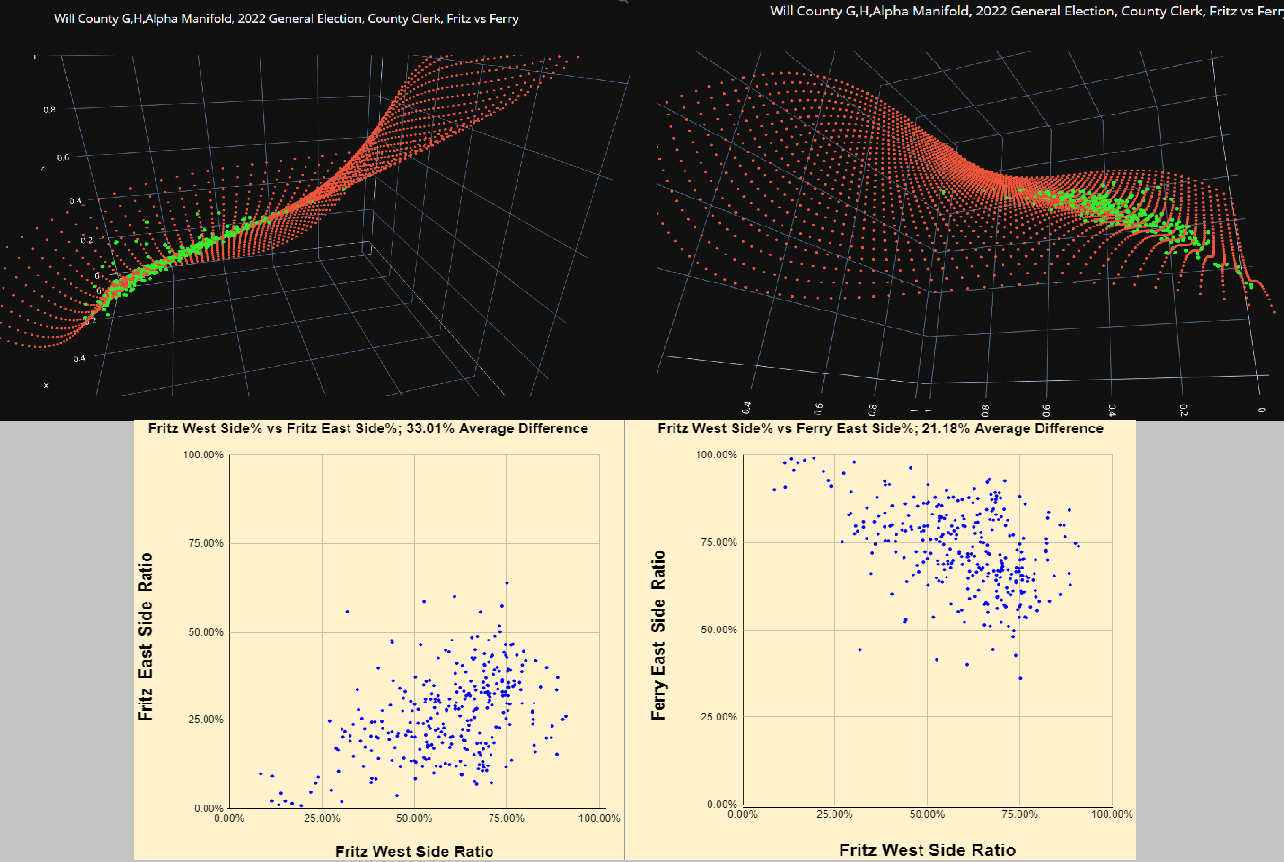
\includegraphics[width=400pt]{will county latex.png}
\end{center}
\end{figure}
\newpage
In the next figure we the Atlanta (Georgia) 2020 Election of Trump vs Biden. The definitions for \textbf{S,T,U,V} are the same as they are for Clark and Washoe Counties Nevada, viz. \textbf{S,T,U,V} are Trump's Early Vote, Biden's Early, Trump's Mail-in Vote and Biden's Mail-in Vote across the precincts of the counties making up Atlanta. We again yield a cubic manifold for $alpha_{1}$ in terms of $g_{1}$ and $h_{1}$ for Atlanta Georgia, just like in Will County Illinois. Yet---in the Clark and Washoe Counties (Nevada), in 2020 and 2022, we get a perfectly flat plane using the same definitions of \textbf{S,T,U,V}, and being a flat plane, it makes $lambda_{1}$ constant over the precincts of Clark and Washoe, allowing us to explain the rig using only vote totals (that is, we can calculate Biden's Mail-in Vote knowing only the total number of ballots cast and Trump's Early Vote).

What makes this even stranger is that you only need a sample of size of a few precincts to predict the remaining 1200 precincts. If these facts are not sufficient to assert that the election was rigged (beyond all reasonable doubt), then what kind of mathematical facts would be? Remember, that if you're planning on writing a ``stunning refutation of Edward Solomon's claims" you're going to have to explain why we find curved manifolds in some battleground states and flat manifolds in other battleground states, and why these manifolds only appear in the West vs East Orientation (but not in the natural North vs South Orientations). Here are the links to the 2020 Election for Trump vs Biden in Atlanta: \url{https://docs.google.com/spreadsheets/d/1HoOpkuWDnfTG-mezrCBd7t04gb0YkhA5YDMzcgK-MVo/edit?usp=sharing} and \url{https://plotly.com/~EKSolomon/104/}
\begin{figure}[bp!]
\begin{center}
\caption{G,H, Alpha Manifold of 2020 Atlanta, Trump vs Biden}
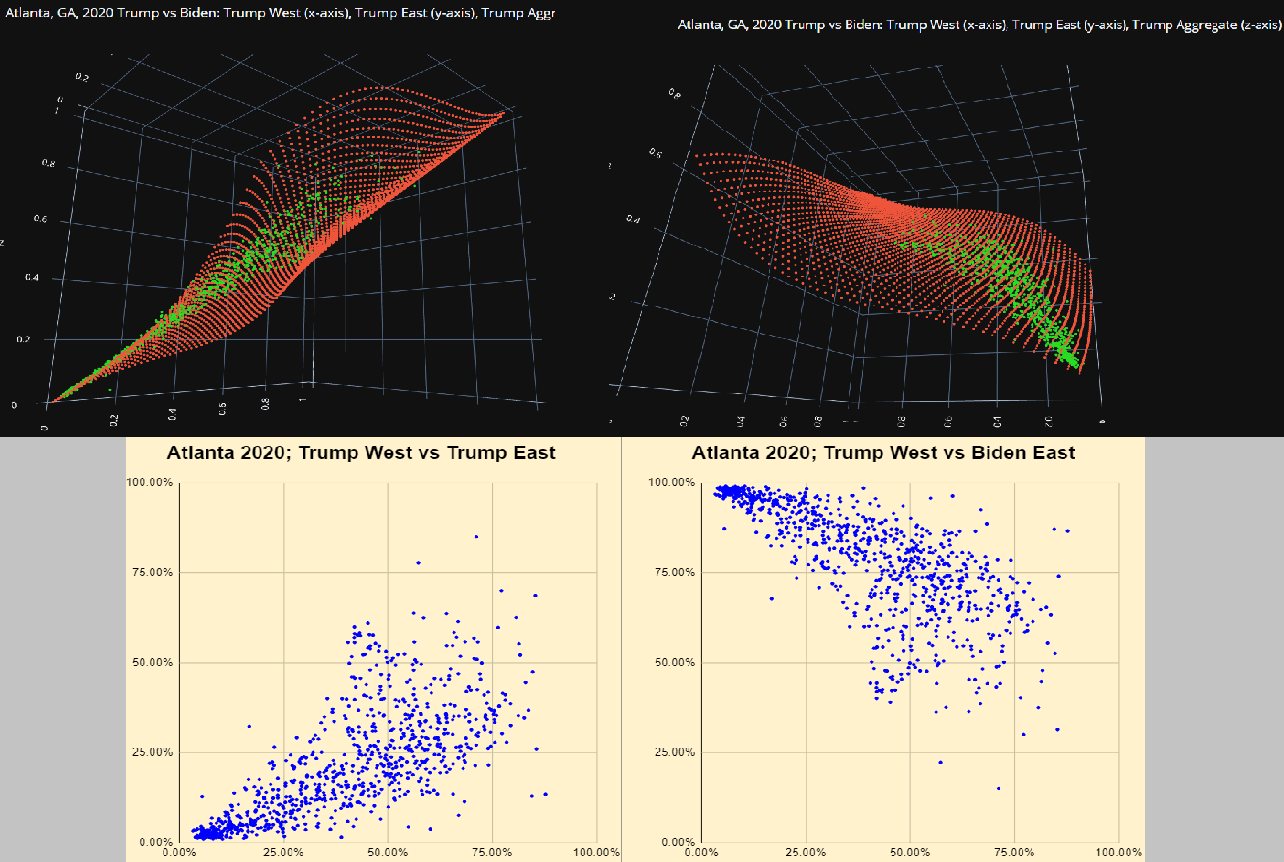
\includegraphics[width=300pt]{atlanta latex.png}
\end{center}
\end{figure}
\newpage
\begin{corollary}[The Expected 3D Boundaries of Omega]
Assuming that the vote totals are positive integers, then:

Given $\mu_{8}=\mu_{A}$ and $\sigma_{8}=\sigma_{A}$, which is the mean and standard deviation of $\alpha_{1}$, and $\mu_{9}=\mu_{L}$ and $\sigma_{9}=\sigma_{L}$, which is the mean and standard deviation of $\lambda_{1}$, for some disjoint \textbf{S,T,U} and \textbf{V} denomination of the Analyzed Precincts, then from the Twixt Lemma we know that roughly 95\% of the $\Omega_{1,b}$ values are bounded between the two planes:

For the Diagonal vs Diagonal Orientation:
Case One:  For when $m_{1} \le n_{1}$, then:
$$(\mu_{8}-2\sigma_{8})m_{1,b} \le \Omega_{1} \le (1-\mu_{8}+2\sigma_{8})n_{1,b}$$
AND
$$(\mu_{8}+2\sigma_{8})m_{1,b} \le \Omega_{1} \le (1-\mu_{8}-2\sigma_{8})n_{1,b}$$

Case Two: For when $n_{1} < m_{1}$, then:
$$(1-\mu_{8}-2\sigma_{8})n_{1,b} < \Omega_{1} < (\mu_{8}+2\sigma_{8})m_{1,b}$$
AND
$$(1-\mu_{8}+2\sigma_{8})n_{1,b} < \Omega_{1} < (\mu_{8}-2\sigma_{8})m_{1,b}$$

Or more succinctly (for Case 1 and Case 2 respectively):\\
$\Omega_{1} \le +n_{1}+(2\sigma_{8}-\mu_{8})(m_{1}+n_{1})$ AND $\Omega_{1} \le +n_{1}-(2\sigma_{8}-\mu_{8})(m_{1}+n_{1})$\\
$\Omega_{1} \le -n_{1}+(\mu_{8}-2\sigma_{8})(m_{1}+n_{1})$ AND $\Omega_{1} \le -n_{1}+(\mu_{8}+2\sigma_{8})(m_{1}+n_{1})$

For the West vs East Orientation:
Case One:  For when $g_{1} \le h_{2}$, then (notice that $h_{2}$ was invoked):
$$(\mu_{9}-2\sigma_{9})g_{1,b} \le \Omega_{1} \le (1-\mu_{9}+2\sigma_{9})h_{2,b}$$
AND
$$(\mu_{9}+2\sigma_{9})g_{1,b} \le \Omega_{1} \le (1-\mu_{9}-2\sigma_{9})h_{2,b}$$

Case Two: For when $h_{2} < g_{1}$, then:
$$(1-\mu_{9}-2\sigma_{9})h_{2,b} < \Omega_{1} < (\mu_{9}+2\sigma_{9})g_{1,b}$$
AND
$$(1-\mu_{9}+2\sigma_{9})h_{2,b} < \Omega_{1} < (\mu_{9}-2\sigma_{9})g_{1,b}$$

Or more succinctly (for Case 1 and Case 2 respectively):\\
$\Omega_{1} \le +h_{2}+(2\sigma_{9}-\mu_{9})(g_{1}+h_{2})$ AND $\Omega_{1} \le +h_{2}-(2\sigma_{9}-\mu_{9})(g_{1}+h_{2})$\\
$\Omega_{1} \le -h_{2}+(\mu_{9}-2\sigma_{9})(g_{1}+h_{2})$ AND $\Omega_{1} \le -h_{2}+(\mu_{9}+2\sigma_{9})(g_{1}+h_{2})$
\end{corollary}
\newpage
\begin{corollary}[The Expected 3D Boundaries of Lambda]
Assuming that the vote totals are positive integers, then:

Given $\mu_{7}=\mu_{O}$ and $\sigma_{7}=\sigma_{O}$, which is the mean and standard deviation of $\Omega_{1}$, and $\mu_{8}=\mu_{A}$ and $\sigma_{8}=\sigma_{A}$, which is the mean and standard deviation of $\alpha_{1}$, for some disjoint \textbf{S,T,U} and \textbf{V} denomination of the Analyzed Precincts, then from the Twixt Lemma we know that roughly 95\% of the $\lambda_{1,b}$ values are bounded between the two planes:

For the North vs South Orientation:
Case One:  For when $x_{1} \le y_{2}$, then (notice that $y_{2}$ wsa invoked):
$$(\mu_{7}-2\sigma_{7})x_{1,b} \le \lambda_{1} \le (1-\mu_{7}+2\sigma_{7})y_{2,b}$$
AND
$$(\mu_{7}+2\sigma_{7})x_{1,b} \le \lambda_{1} \le (1-\mu_{7}-2\sigma_{7})y_{2,b}$$

Case Two: For when $y_{2} < x_{2}$, then:
$$(1-\mu_{7}-2\sigma_{7})y_{2,b} < \lambda_{1} < (\mu_{7}+2\sigma_{7})x_{1,b}$$
AND
$$(1-\mu_{7}+2\sigma_{7})y_{2,b} < \lambda_{1} < (\mu_{7}-2\sigma_{7})x_{1,b}$$

Or more succinctly (for Case 1 and Case 2 respectively):\\
$\lambda_{1} \le +y_{2}+(2\sigma_{7}-\mu_{7})(x_{1}+y_{2})$ AND $\lambda_{1} \le +y_{2}-(2\sigma_{7}-\mu_{7})(x_{1}+y_{2})$\\
$\lambda_{1} \le -y_{2}+(\mu_{7}-2\sigma_{7})(x_{1}+y_{2})$ AND $\lambda_{1} \le -y_{2}+(\mu_{7}+2\sigma_{7})(x_{1}+y_{2})$

For the Diagonal vs Diagonal Orientation:
Case One:  For when $m_{1} \le n_{2}$, then:
$$(\mu_{8}-2\sigma_{8})m_{1,b} \le \lambda_{1} \le (1-\mu_{8}+2\sigma_{8})n_{2,b}$$
AND
$$(\mu_{8}+2\sigma_{8})m_{1,b} \le \lambda_{1} \le (1-\mu_{8}-2\sigma_{8})n_{2,b}$$

Case Two: For when $n_{2} < g_{1}$, then:
$$(1-\mu_{8}-2\sigma_{8})n_{2,b} < \lambda_{1} < (\mu_{8}+2\sigma_{8})m_{1,b}$$
AND
$$(1-\mu_{8}+2\sigma_{8})n_{2,b} < \lambda_{1} < (\mu_{8}-2\sigma_{8})m_{1,b}$$

Or more succinctly (for Case 1 and Case 2 respectively):\\
$\lambda_{1} \le +n_{2}+(2\sigma_{8}-\mu_{8})(m_{1}+n_{2})$ AND $\lambda_{1} \le +n_{2}-(2\sigma_{8}-\mu_{8})(m_{1}+n_{2})$\\
$\lambda_{1} \le -n_{2}+(\mu_{8}-2\sigma_{8})(m_{1}+n_{2})$ AND $\lambda_{1} \le -n_{2}+(\mu_{8}+2\sigma_{8})(m_{1}+n_{2})$
\end{corollary}
\newpage
\begin{corollary}{The Invariant Aggregate Lemma}\\
As the standard deviation of $Omega_{1}$ goes to zero (as $\sigma_{7}$ goes to zero), the 3D scatter clouds of $x_{1,b}$ (or $x_{2,b}$) and $y_{1,b}$ (or $y_{2,b}$) and $\alpha_{1,b}$ (or $\alpha_{2,b}$) collapse to a flat plane, regardless of the two dimensional distribution of $x_{1,b}$ and $y_{1,b}$ within the unit square, such that:

$\alpha_{1}=x_{1,b}\mu_{7}+(1-\mu_{7})y_{1,b}$, where $\mu_{7}$ is the mean value of $Omega_{1}$.

As the standard deviation of $Omega_{1}$ goes to zero (as $\sigma_{7}$ goes to zero), the 3D scatter clouds of $x_{1,b}$ (or $x_{2,b}$) and $y_{2,b}$ (or $y_{1,b}$) and $\lambda_{1,b}$ (or $\lambda_{2,b}$) collapse to a flat plane, regardless of the two dimensional distribution of $x_{1,b}$ and $y_{2,b}$ within the unit square, such that:

$\lambda_{1}=x_{1,b}\mu_{7}+(1-\mu_{7})y_{2,b}$, where $\mu_{7}$ is the mean value of $Omega_{1}$.

As the standard deviation of $alpha_{1}$ goes to zero (as $\sigma_{8}$ goes to zero), the 3D scatter clouds of $m_{1,b}$ (or $m_{2,b}$) and $n_{1,b}$ (or $n_{2,b}$) and $\Omega_{1,b}$ (or $\Omega_{2,b}$) collapse to a flat plane, regardless of the two dimensional distribution of $m_{1,b}$ and $n_{1,b}$ within the unit square, such that:

$\Omega_{1}=m_{1,b}\mu_{8}+(1-\mu_{8})n_{1,b}$, where $\mu_{8}$ is the mean value of $Omega_{1}$.

As the standard deviation of $alpha_{1}$ goes to zero (as $\sigma_{8}$ goes to zero), the 3D scatter clouds of $m_{1,b}$ (or $m_{2,b}$) and $n_{2,b}$ (or $n_{1,b}$) and $\lambda_{1,b}$ (or $\lambda_{2,b}$) collapse to a flat plane, regardless of the two dimensional distribution of $m_{1,b}$ and $n_{2,b}$ within the unit square, such that:

$\lambda_{1}=m_{1,b}\mu_{8}+(1-\mu_{8})n_{2,b}$, where $\mu_{8}$ is the mean value of $Omega_{1}$. 

As the standard deviation of $lambda_{1}$ goes to zero, \textbf{as it does in Clark and Washoe Counties Nevada} (as $\sigma_{9}$ goes to zero), the 3D scatter clouds of $g_{1,b}$ (or $g_{2,b}$) and $h_{1,b}$ (or $h_{2,b}$) and $\alpha_{1,b}$ (or $\alpha_{2,b}$) collapse to a flat plane, regardless of the two dimensional distribution of $g_{1,b}$ and $h_{1,b}$ within the unit square, such that:

$\alpha_{1}=g_{1,b}\mu_{9}+(1-\mu_{9})h_{1,b}$, where $\mu_{9}$ is the mean value of $Omega_{1}$.

As the standard deviation of $lambda_{1}$ goes to zero, \textbf{as it does in Clark and Washoe Counties Nevada} (as $\sigma_{9}$ goes to zero), the 3D scatter clouds of $g_{1,b}$ (or $g_{2,b}$) and $h_{2,b}$ (or $h_{1,b}$) and $\Omega_{1,b}$ (or $\Omega_{2,b}$) collapse to a flat plane, regardless of the two dimensional distribution of $g_{1,b}$ and $h_{2,b}$ within the unit square, such that:

$\Omega_{1}=g_{1,b}\mu_{9}+(1-\mu_{9})h_{2,b}$, where $\mu_{9}$ is the mean value of $Omega_{1}$.
\end{corollary}
\newpage
\begin{corollary}{The Invariant Aggregate Integer Dilemma}\\
Let $z_{b}=s_{b}+t_{b}+u_{b}+v_{b}$ for each data point (each precinct).
Given $\mu_{7}, \mu_{8}, \mu_{9}$ as the mean values of $\Omega_{1,b}, \alpha_{1,b}, \lambda_{1,b}$ across the precincts (respectively), then:

As the standard deviation of $\Omega_{1}$ goes to zero (as $\sigma_{7}$ goes to zero), one can calculate:\\
$t_{b}$ knowing only $z_{b}$ and $s_{b}$, in the form of $t_{b}=\mu_{7}z_{b}-s_{b}$.\\
$s_{b}$ knowing only $z_{b}$ and $t_{b}$, in the form of $s_{b}=\mu_{7}z_{b}-t_{b}$.\\
$z_{b}$ knowing only $s_{b}$ and $t_{b}$, in the form of $z_{b}=(\frac{1}{\mu_{7}})(s_{b}+t_{b})$.\\
$v_{b}$ knowing only $z_{b}$ and $u_{b}$, in the form of $v_{b}=\mu_{7}z_{b}-u_{b}$.\\
$u_{b}$ knowing only $z_{b}$ and $v_{b}$, in the form of $u_{b}=\mu_{7}z_{b}-v_{b}$.\\
$z_{b}$ knowing only $u_{b}$ and $v_{b}$, in the form of $z_{b}=(1-\frac{1}{\mu_{7}})(u_{b}+v_{b})$.\\
More generally, as  $\sigma_{7}$ goes to zero, the ballots flow equally by proportion from $s_{b}$ to $t_{b}$ and from $u_{b}$ to $v_{b}$ as $\alpha_{b}$ increases.

As the standard deviation of $\alpha_{1}$ goes to zero (as $\sigma_{8}$ goes to zero), one can calculate:\\
$u_{b}$ knowing only $z_{b}$ and $s_{b}$, in the form of $u_{b}=\mu_{8}z_{b}-s_{b}$.\\
$s_{b}$ knowing only $z_{b}$ and $u_{b}$, in the form of $s_{b}=\mu_{8}z_{b}-u_{b}$.\\
$z_{b}$ knowing only $s_{b}$ and $u_{b}$, in the form of $z_{b}=(\frac{1}{\mu_{8}})(s_{b}+u_{b})$.\\
$v_{b}$ knowing only $z_{b}$ and $t_{b}$, in the form of $v_{b}=\mu_{8}z_{b}-t_{b}$.\\
$t_{b}$ knowing only $z_{b}$ and $v_{b}$, in the form of $t_{b}=\mu_{8}z_{b}-v_{b}$.\\
$z_{b}$ knowing only $t_{b}$ and $v_{b}$, in the form of $z_{b}=(1-\frac{1}{\mu_{8}})(t_{b}+v_{b})$.
More generally, as  $\sigma_{8}$ goes to zero, the ballots flow equally by proportion from $s_{b}$ to $u_{b}$ and from $t_{b}$ to $v_{b}$ as $\Omega_{b}$ increases.

As the standard deviation of $\lambda_{1}$ goes to zero (as $\sigma_{9}$ goes to zero), one can calculate:\\
$v_{b}$ knowing only $z_{b}$ and $s_{b}$, in the form of $v_{b}=\mu_{9}z_{b}-s_{b}$.\\
$s_{b}$ knowing only $z_{b}$ and $v_{b}$, in the form of $s_{b}=\mu_{9}z_{9}-v_{b}$.\\
$z_{b}$ knowing only $s_{b}$ and $v_{b}$, in the form of $z_{b}=(\frac{1}{\mu_{9}})(s_{b}+v_{b})$.\\
$t_{b}$ knowing only $z_{b}$ and $u_{b}$, in the form of $t_{b}=\mu_{9}z_{b}-u_{b}$.\\
$u_{b}$ knowing only $z_{b}$ and $t_{b}$, in the form of $u_{b}=\mu_{9}z_{b}-t_{b}$.\\
$z_{b}$ knowing only $u_{b}$ and $t_{b}$, in the form of $z_{b}=(1-\frac{1}{\mu_{9}})(u_{b}+t_{b})$.\\
More generally, as  $\sigma_{9}$ goes to zero, the ballots flow equally by proportion from $s_{b}$ to $v_{b}$ and from $u_{b}$ to $t_{b}$ as $\alpha_{b}$ increases, \textbf{as it is in all 1286 precincts in two distant counties, Clark and Washoe, on opposite sides of the State of Nevada, where Trump's Early vote (s) flows into Biden's Mail-in vote (v), at the same rate as Trump's Mail-in Vote (u) flows into Biden's Early Vote (t), as Trump's Aggregate Percentage (alpha) increases over the precincts.}
\end{corollary}
\newpage
The Invariance Aggregate Lemmas are a critical tool in the Prosecution's toolkit, since no meaningful Quantile Simulations can be performed when either $\alpha, \Omega$ or $\lambda$  are invariant across the precincts, because whether or not the data analyst performs a simulation from the North vs South, East vs West or Diagonal vs Diagonal perspectives, the invariance of any aggregate will have imprinted itself upon all three of those perspectives.

Thus, all simulations will be that of an unchanging parameter. 

No matter how many times one simulates the elections of Clark County in Nevada, they will always get an $R^2$>0.99 for the manifold of regression of either $g,h$ or $\alpha$ from the remaining two, because $\lambda$ will always be invariant (63.5\%) in the simulations, compelling, in every precinct:

$\alpha_{1,b}=0.65g_{1,b}+0.35h_{1,b}$ and $g=\frac{\alpha_{1,b}-0.35h_{1,b}}{0.65}$ and $h=\frac{\alpha_{1,b}-0.65g_{1,b}}{0.35}$

In this situation the \textbf{\textcolor{red}{Burden of the Prosecution}} is not to show that the $R^2$ of the election result is above or below the Five-Sigma Rule via Quantile Simulations (which is how one must prove that Maricopa 2020 and 2022 were rigged), but rather to convince the \textbf{Jury} that the Invariance of Lambda across 1200 precincts, in two counties, on opposite sides of the State of Nevada, is absurd by definition; while it is the \textbf{\textcolor{red}{Burden of the Defense}} to convince the \textbf{Jury} that is perfectly normal for the proportion of two disjoint ballot sets to be uniform across 1200 precincts in two distant counties on opposite sides of the State of Nevada (I would much prefer to be the prosecution in this case!).

In other words, if I told the Jury, "What are chances of Trump's Early Vote and Biden's Mail-in Vote being 63.5\% of all ballots cast at each of the 1286 precincts, in two highly populated and demographically different counties on opposite sides of the State of Nevada? No one knows for sure the exact chance of this event, but we all know intuitively that whatever that chance may be, it is effectively zero, and never happen in real life. How could millions of voters across two counties make such a uniform decision to split their ballots equally between the mathematically abstract East and West Sides of the precinct?" 

How do you think the Jury would rule?

Do you think you could say anything to the Jury that would make them rule otherwise? If not, I suggest you don't write a ``stunning refutation of Edward Solomon's claims."
\newpage
\subsection{The Hyperbolic Reflection Theorem}
Before we move on to the following chapters, there is one piece of pure mathematical theory that we must cover. This final theorem is what allows us to restore an election to its original state prior to the tabulations being manipulated by Lambda Invariant Manifold.
\begin{theorem}{Hyperbolic Reflection Theorem}\\
The Sixth Law states that:
$$y_{1}=\lambda_{2}-\zeta^{-1}(\lambda_{1}-x_{1})$$
Which can rewritten as:
$$y_{2}=\lambda_{1}-\zeta^{-1} (\lambda_{1}-x_{1})$$

Which, in the case of Clark County, says that Biden's Mail-in Percentage, $y_{2}$ is the vertical reflection of Trump's Early Percentage, $x_{1}$, over the line (value) of $\lambda_{1}$, scaled inversely proportional to $\zeta$, which is the Proportion of Mail-in to Early Votes.

Hence if $\lambda_{1}$ is constant over the precincts (regardless of their sorting) and the trajectory of $\zeta$ declines over the quantiles of $x_{1}$ (when the precincts are sorted by Trump's Early Percentage), then it follows that the Sixth Law will induce a dynamic rotation matrix upon the trajectory of $y_{2}$ (Biden's Mail-in Vote), since Trump's Early Percentage will be reflected over an invariant flat horizontal line (the value of $\lambda$ in each precinct), at a hyperbolically increasing scale, to produce Biden's Mail-in Percentage, causing the natural linear relationship between Trump's Early Percentage and Biden's Mail-in Percentage to deform into a hyperbolic relationship (that can be well approximated by quartic).
\end{theorem}
\newpage
\subsection{The Two Common Sense Assumptions}

Suppose you asked a fifth grader: ``If I was so hated at specific place, that I got 0\% of the election day vote, what percentage of the mail-in vote do you think I would get."

The Fifth Grader would answer correctly: "About 0\%."

Suppose you asked a fifth grader: ``If I was so loved at specific place, that I got 100\% of the election day vote, what percentage of the mail-in vote do you think I would get."

The Fifth Grader would answer correctly: ``About 100\%."

Suppose you asked a fifth grader: ``If I was there was a tie at specific place, such that I got 50\% of the election day vote, what percentage of the mail-in vote do you think I would get."

The Fifth Grader would answer (incorrectly): ``About 50\%." However, the Fifth Grader's answer is only incorrect in an election where we expect Democrats to prefer to vote by mail, otherwise he'd be right on.

You now draw the coordinates of his three answers, (0,0), (50,50) and (100,100). You tell him to connect the three dots. He will draw a straight line, at 45 degrees from the origin through those three points.

You now ask the Fifth Grader: ``What do you think that line means?" The Fifth Grader would answer incorrectly: ``That your mail-in percentage will be roughly equal to your election day percentage in each precinct."

A Tenth Grader would produce the same answer in a little more detail: ``That although it would be unusual for your election day percentage and mail-in percentage to be the EXACT same in every precinct, it would also be unusual for them to not be strongly correlated along that 45 degree line."

An undergraduate would say (incorrectly): ``That in general, party affiliation, such as Democrat or Republican, shouldn't have a significant effect on a candidate's performance on election day and in the mail." The undergraduate would then go on to take a linear regression of the mail-in percentage in terms of the election day percentage (like Professor Grimmer did in the Gilbert vs Lombardo case) and be surprised to see that the slope wasn't anywhere near 45 degrees. This is because the linear regression of y from x is not the same as the eigenvector of x+iy.

The graduate student would say (correctly): ``That the eigenvector of the election day and mail-in coordinates would be close to forty-five degrees in a fair election, such that, even if one particular political party had an advantage in one form of voting, that advantage would be relatively constant over the dataset, such that general relationship, or eigenvector, would be at or close to 45 degrees, excluding the corners of the unit square, where x approaches 0 and 1, where y must also converge on 0 and 1 respectively."

The Mainstream Media and Election Abusers would say: ``But Democrats vote overwhelming by mail, so you're all wrong---and pay no heed to the man behind the curtain drawing up those manifolds! And pay no attention that Republicans also vote overwhelming by mail for the establishment candidates (such as Lombardo) in their primaries! Pay no heed to the fact the Democrats vote more by mail in Republican Precincts than they in Democrat precincts!"
\begin{definition}{The First Common Sense Assumption}

Assuming that $x$ and $y$ represent the percentage of ballots cast for the same candidate, that the general trajectories of $x$ and $y$ should be parallel in respect to each other, otherwise we would result with otherworldly scenarios where a candidate receives 0\% of the election day vote at a precinct, but somehow receives 40\% of the mail-in vote at the same precinct.
\end{definition}

\begin{definition}{The First Common Sense Assumption, PhD Level}

Assuming that $x$ and $y$ represent the percentage of ballots cast for the same candidate in two distinct modes, and that the mean value of $\Omega$ is between 25\% and 75\%, such that both the modes being represented by $x$ and $y$ contain at least 25\% of the electorate, that the eigenvector of the $(x,y)$ coordinates should be at or close to 45 degrees, and since $\alpha$ must exist between $x$ and $y$, it follows that the eigenvectors both the $(x,\alpha)$ and $(\alpha,y)$ coordinates should also be at 45 degrees, even if there is a mean negative difference between the expected $x$ and $y$ trajectories.
\end{definition}

Thenceforth, when you see the phrase ``The First Common Sense Assumption" in quotation marks, the above is the definition of that phrase. 

I am sure you are currently wondering ``What is the Second Common Sense Assumption." It is the assumption that both the ordinary layperson and astute mathematician would make in an election where ``Democrats prefer to Vote by Mail." 

The First Common Sense Assumption is \textcolor{red}{NOT} incompatible with an election where a particular party prefers to cast their ballots in a particular mode. Remember that $m_{b}=\frac{Republican Early}{Republican Early + Republican Mail}$ or $m_{b}=\frac{Republican Election Day}{Republican Election Day + Republican Mail}$; and that, $n_{b}=\frac{Democrat Early}{Democrat Early + Democrat Mail}$ or $n_{b}=\frac{Democrat Election Day}{Democrat Election Day + Democrat Mail}$.

Thus the $m$ and $n$ percentages measure the preference of each party's voter base to cast their ballot by one mode or another. We now ask our Fifth Grader the following question.

``In Clark County, Democrats have a 35\% chance, $n_{b}$, to cast their ballot Early, as opposed to by Mail, where Republicans have 62\%, $m_{b}$, chance to cast their ballot Early. Would you expect these chances to change significantly accordingly to exact location in which people live in Clark County?" The Fifth Grader will respond ``No, why would Democrats or Republicans have different preferences from other Democrats or Republicans in the same county? I can't think of any reason why."

The graduate student will respond ``The mean percentage of $m$ and $n$ will be flat across the precincts when sorted by either $x,y$ or $\alpha$. The only time we would expected to see a significant rise or fall of both $m$ and $n$ is if---and only if---a large \textbf{consecutive} sequence of precincts along the quantiles of $x,y$ or $\alpha$ had a uniform and wildly different geography or demographic from the other precincts in the same county, and such that, when the precincts exit this region of the $x,y$ or $\alpha$ quantiles, that the expected trajectory of $m$ and $n$ shall return to their flat trajectory at $m=0.62$ and $n=0.35$ in the example you provided for me of Clark County. In general, the trajectory of $m$ and $n$ should be flat, especially if the mean value of $\Omega$ is bounded between 25\% and 75\%, since both forms of voting represent a sample size of at least 25\% of an Electorate with hundreds of thousands, if not millions, of voters."

\begin{definition}{The Second Common Sense Assumption}

That the preference of Republicans and Democrats to vote on election day, or to vote early or vote by mail, should be relatively uniform over the precincts of the same county.
\end{definition}

\begin{definition}{The Second Common Sense Assumption, PhD Level}

Since the quantiles of $x,y$ and $\alpha$ ignore geography and demographics, that the trajectories of $m$ and $n$ should be flat over the quantiles of $x,y$ and $\alpha$, assuming that the mean value of $\Omega$ is bounded between 25\% and 75\%, since this implies that the two distinct modes of voting represented by $x$ and $y$ both contain a sufficiently large sample size of the electorate making up the modes respective to $x$ and $y$. 

More specifically, if neither $m$ nor $n$ are flat across the quantiles of $x,y$ or $\alpha$, then they must remain parallel, since this would imply a continuous change in a particular and politically neutral demographic (such as age) over the quantiles of $x,y$ and $\alpha$, which should effect $m$ and $n$ equally, since politically neutral demographics (such as age), should affect the electorate of both parties equally, and politically charged demographic variables have already been accounted for by the mean difference between $m$ and $n$.
\end{definition}
Thenceforth when you see the term ``The Second Common Sense Assumption" the above is the definition of that term. Below is the link to Bard's Response to this same question: \url{https://g.co/bard/share/681eaac9df9c}
\newpage
The below picture is how both ordinary people (left) and mathematicians (right) depict the First and Second Common Sense Assumptions. Notice the general similarity.

The ordinary person tends to be quite confident that the picture they drew accurately represents a fair election where Democrats prefer to vote by mail from $0.1<x<0.9$, even though they often admit they don't know how to deal with the corners of the unit square where either $x<0.1$ or $x>0.9$.

When I question math students and professors on this topic, they also draw the same general picture for the range of $0.1<x<0.9$, in fact the $m,n$ and $\Omega$ trajectories are the same when both ordinary people and academics draw them. As for dealing with the corners of the unit square,  they all agree that the local eigenvector will be at 45 degrees from $0.3<x<0.7$, and will start to bend upwards from $0.7<x<0.9$, and downwards from $0.1<x<0.3$. 

I then provide the following equation to them (and display it) and ask them if it matches what they'd expect in a fair election where Democrats prefer to vote by mail with a 8\% lead in the mail-in percentage. Almost all agree upon seeing the trajectory (and the rest agree after a short discussion!), and furthermore all agree that the actual corners of the unit square will behave erratically (thus the ordinary person was right in their refusal to draw the corner behavior).
$$v=A\left(\left(u-\frac{\sqrt{2}}{2}\right)^4-k\right); u=+x\cos{\frac{\pi}{4}}+y\sin{\frac{\pi}{4}}; v=-x\sin{\frac{\pi}{4}}+y\cos{\frac{\pi}{4}}$$
\begin{figure}[bp!]
\begin{center}
\caption{How People Draw an Election where Democrats Prefer to Vote by Mail.}
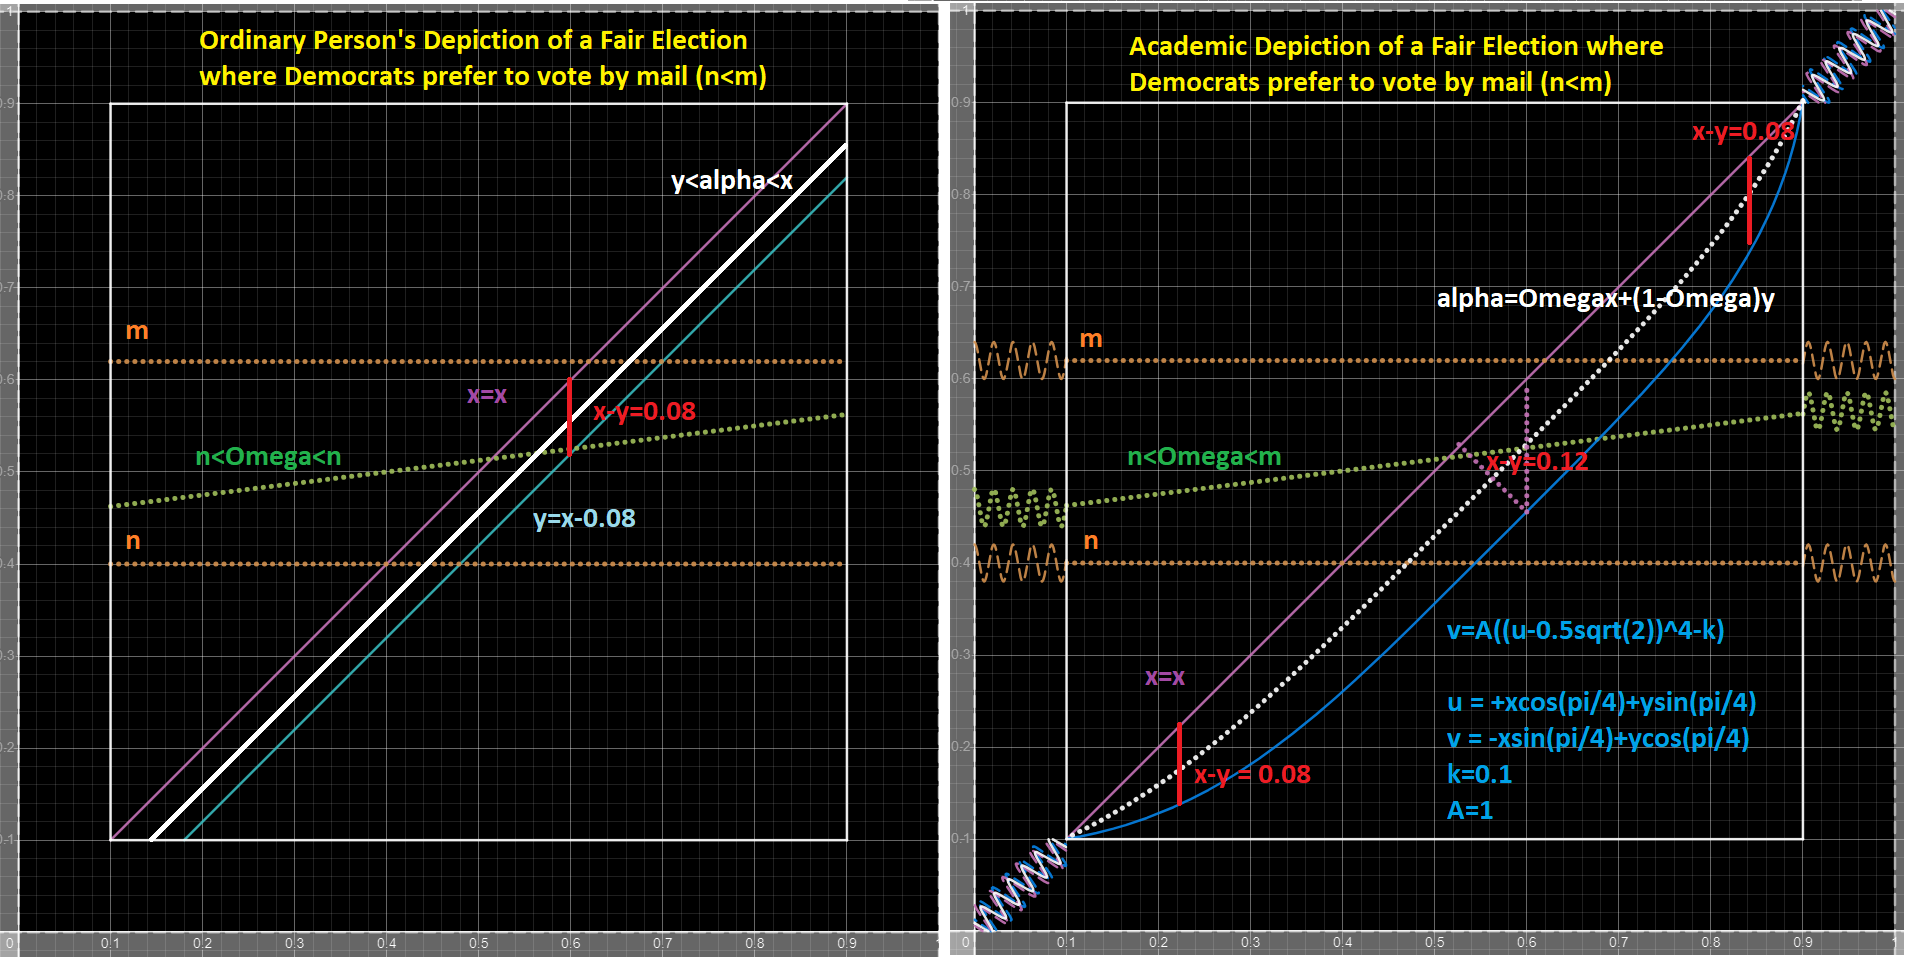
\includegraphics[width=350pt]{Fifth Grader vs Grad.png}
\end{center}
\end{figure}
\newpage
\subsection{Bard and ChatGPT's Verdict on the Two Common Sense Assumptions}
Bard's Response:\\
\url{https://g.co/bard/share/108cdda7e149}

ChatGPT's response:\\
\url{https://chat.openai.com/share/3ab88b2e-515c-475b-bc36-0e3067ba5cb0}

Both AI's were asked the same exact question (where z takes the place of $\alpha$ and p takes the place of $\Omega$ so I could write the question without special formatting):

\textit{``Let A be Alice's Election Day Vote (who is a Republican) at a precinct, let B be Bob's Election Day Vote (who is a Democrat) at the same precinct, let C be Alice's Mail-in Vote at the same precinct, and let D be Bob's Mail in Vote, at the same precinct.}

\textit{Let m=A/(A+C) be the percentage of Republicans that prefer to vote on election day at that precinct.}

\textit{Let n=B/(B+D) be the percentage of Democrats that prefer to vote on election day at that precinct.}

\textit{Let z = (A+C)/(A+B+C+D) be Alice's Aggregate Percentage at that precinct.}

\textit{I would now like you to evaluate my stance on these three questions:}

\textit{Question One: Since Democrats prefer to vote by mail, we expect $n<m$ across a dataset of precincts. However, if the precincts are sorted by either their x,y, or z values, we should expect the trajectories of m and n to be flat over the quantiles of x,y and z since the quantiles of x,y, and z ignore any sorting geography and demographics, correct?}

\textit{Additional context for Question One: This of course is assuming that p=(A+B)/(A+B+C+D) has a mean value between 25\% and 75\%, such that the election day vote and the mail-in vote both represent at least 25\% of the electorate (if the mean value of p goes outside these boundaries, then either the election day vote or the mail-in vote may not fairly represent the entire voting base).}

\textit{Question Two:  Also, assuming that the mean value of p remains within the boundaries of 25\% to 75\%, we would expect the x and y values to be relatively equal over the precincts, since if someone got 0\% of the election day vote (x), we would expect them to get around 0\% of the mail-in vote, or, if they got 100\% of the election day vote (meaning their opponent got 0\% of the election day vote), then would expect them to get around 100\% of the mail-in vote (meaning we expect their opponent to get around 0\% of the mail-in vote).}

\textit{Thus, even though there might be a small negative difference of x and y across the precincts (say 5\% to 10\%), we would expect the eigenvector of the (x,y) data points to be around 45 degrees, correct?}

\textit{Third Question: Also, is it reasonable to expect the trajectory of x to be parallel to y (that is, even if they have an average mean difference, we still expect a 45 degree relationship between x and y) in a fair election? Without such a relationship, we could end up in situation where a candidate gets 0\% of the election day vote and 0\% of the mail in one precinct, while getting 100\% of the election day vote but only 60\% of the mail-in vote at another precincts (meaning their opponent magically receives 40\% of mail-in vote, even though they got 0\% of the election day vote at the same precinct)."}

Bard's Response was follows:

\textit{``Your stance on these three questions is sound.}

\textbf{Question} One\\
\textit{You are correct that we expect $n<m$ across a dataset of precincts, since Democrats prefer to vote by mail. This is because Democrats are more likely to be young, minority, or have disabilities, all of which are groups that are more likely to vote by mail.}

\textit{If the precincts are sorted by either their x, y, or z values, we should expect the trajectories of m and n to be flat over the quantiles of x, y, and z. This is because the quantiles of x, y, and z ignore any sorting geography and demographics, so they should not affect the relationship between m and n.}

\textbf{Question Two}\\
\textit{You are also correct that we would expect the x and y values to be relatively equal over the precincts. This is because the x and y values are both measures of the same thing: the overall popularity of a candidate. If a candidate is popular, they are likely to do well in both the election day vote and the mail-in vote.}

\textit{Even though there might be a small negative difference of x and y across the precincts, we would still expect the eigenvector of the (x, y) data points to be around 45 degrees. This is because the eigenvector of a data set is a line that best represents the overall trend of the data. In this case, the overall trend of the data is that x and y are relatively equal, so the eigenvector should be around 45 degrees.}

\textbf{Question Three}\\
\textit{Yes, it is reasonable to expect the trajectory of \textcolor{red}{x to be parallel to y in a fair election}. This is because, in a \textcolor{red}{fair election}, the overall popularity of a candidate should \textcolor{red}{not affect how they do in the election day vote or the mail-in vote}. If a candidate is popular, they should do well in both votes.}

\textit{If the trajectory of x is not parallel to y, it could be a sign of voter suppression or \textcolor{red}{fraud}. For example, if a candidate is only able to do well in the election day vote, it could be because they are only able to get their supporters to vote on election day. This could be due to voter suppression efforts that make it difficult for people to vote by mail.}

\textit{\textcolor{red}{Overall, your stance on these three questions is sound}. You have correctly identified the relationships between m, n, x, y, and z, \textcolor{red}{and you have explained why these relationships are important in a fair election."}}

Here is ChatGPT's response:
\textit{``To evaluate your stance on these three questions, let's analyze each question individually:}

\textit{Question One:
Your statement seems to be on the right track. Since Democrats prefer to vote by mail, it is reasonable to expect that the percentage of Democrats who vote on Election Day (n) will be lower than the percentage of Republicans who vote on Election Day (m) across the dataset of precincts. This is because more Democrats choose to vote by mail instead of in person on Election Day.}

\textit{Now, regarding the sorting of precincts by their x, y, or z values: Yes, when sorting precincts based on their x, y, or z values (which seem to represent different factors, like geography, demographics, and voting preferences), the trajectories of m and n should be relatively flat over the quantiles of x, y, and z. This is because the quantiles divide the data into equal parts, disregarding specific characteristics of individual precincts. As a result, the relative proportions of Republicans and Democrats who prefer to vote on Election Day should remain roughly consistent across these quantiles.}

\textit{Additional context: Your assumption about the mean value of p being between 25\% and 75\% is essential to ensure that both the Election Day vote and mail-in vote fairly represent a substantial portion of the electorate.}

\textit{Question Two:
Your reasoning here is sound. If we assume that the mean value of p remains within the boundaries of 25\% to 75\%, it would make sense for the x and y values (percentage of Election Day votes and Mail-in votes for candidates) to be relatively equal over the precincts. This assumption is based on the idea that the proportion of voters who prefer to vote in person (x) should have some level of correlation with the proportion of voters who prefer to vote by mail (y) for a given candidate.}

\textit{While there might be a small negative difference between x and y across precincts, the eigenvector (a mathematical term related to eigenvalues and eigenvectors) that represents the relationship between the (x, y) data points should indeed be around 45 degrees. A 45-degree angle indicates a positive correlation between x and y, meaning that as one increases, the other tends to increase as well.}

\textit{Third Question:
Yes, it is reasonable to expect the trajectory of x to be parallel to y (a 45-degree relationship between x and y) in a fair election. This assumption is based on the idea that the proportion of Election Day votes (x) and the proportion of mail-in votes (y) should be somewhat consistent for a given candidate across different precincts. \textcolor{red}{In a fair election, the relationship between these two voting methods should follow some pattern.}}

\textit{Without such a relationship (i.e., x and y having a random or no correlation), the situation you described could occur, where a candidate gets 0\% of the Election Day vote and 0\% of the mail-in vote in one precinct, but 100\% of the Election Day vote and only 60\% of the mail-in vote in another precinct. This scenario would raise concerns about the fairness and integrity of the election results, \textcolor{red}{as it could indicate potential anomalies or manipulations.}}

\textit{In summary, your stances on these questions seem reasonable and demonstrate an understanding of how the voting preferences of different groups and the relationships between voting methods \textcolor{red}{should behave across precincts in a fair election.}"}

So, not only does both the common man (who would be on a jury) and an academic (who would be an expert witness) on street agree with the two common sense assumptions, but the AI's agree as well. 

\textbf{Do you know why? \textcolor{red}{Because it's common sense!}}
\newpage
\subsection{How the Clark, Washoe and Atlanta (GA) election Defy the Common Sense Assumption}

Let us see if the 2020 Elections of Clark and Washoe Counties, match what we would expect in a Fair Election where Democrats Prefer to Vote by Mail. The term ``Bowshock" in the below diagrams means the maximum distance between the Early Percentage and the trajectory of the Mail-in Percentage.

Notice that $n$ is constantly decreasing which means more Democrats vote by Mail in Republican Precincts. Notice that the distance from $x$ to the trajectory of $y$ keeps increasing, maxing out at 31\%, which means that Republicans suffer more in the mail the better they perform in the Early Vote. Such monstrosities are the \textbf{forced} result of an election that was rigged with a flat plane of $g,h,\alpha$ (setting $\lambda$ constant over the precincts), due to the Twenty Laws and Forty Isometries. We'll cover this in the final section of this chapter.
\begin{figure}[bp!]
\begin{center}
\caption{Why is N decreasing with X? Why is Y diverging from X? Why does Biden get Magic Mail-in Votes when he gets 0\% of the Early Vote?}
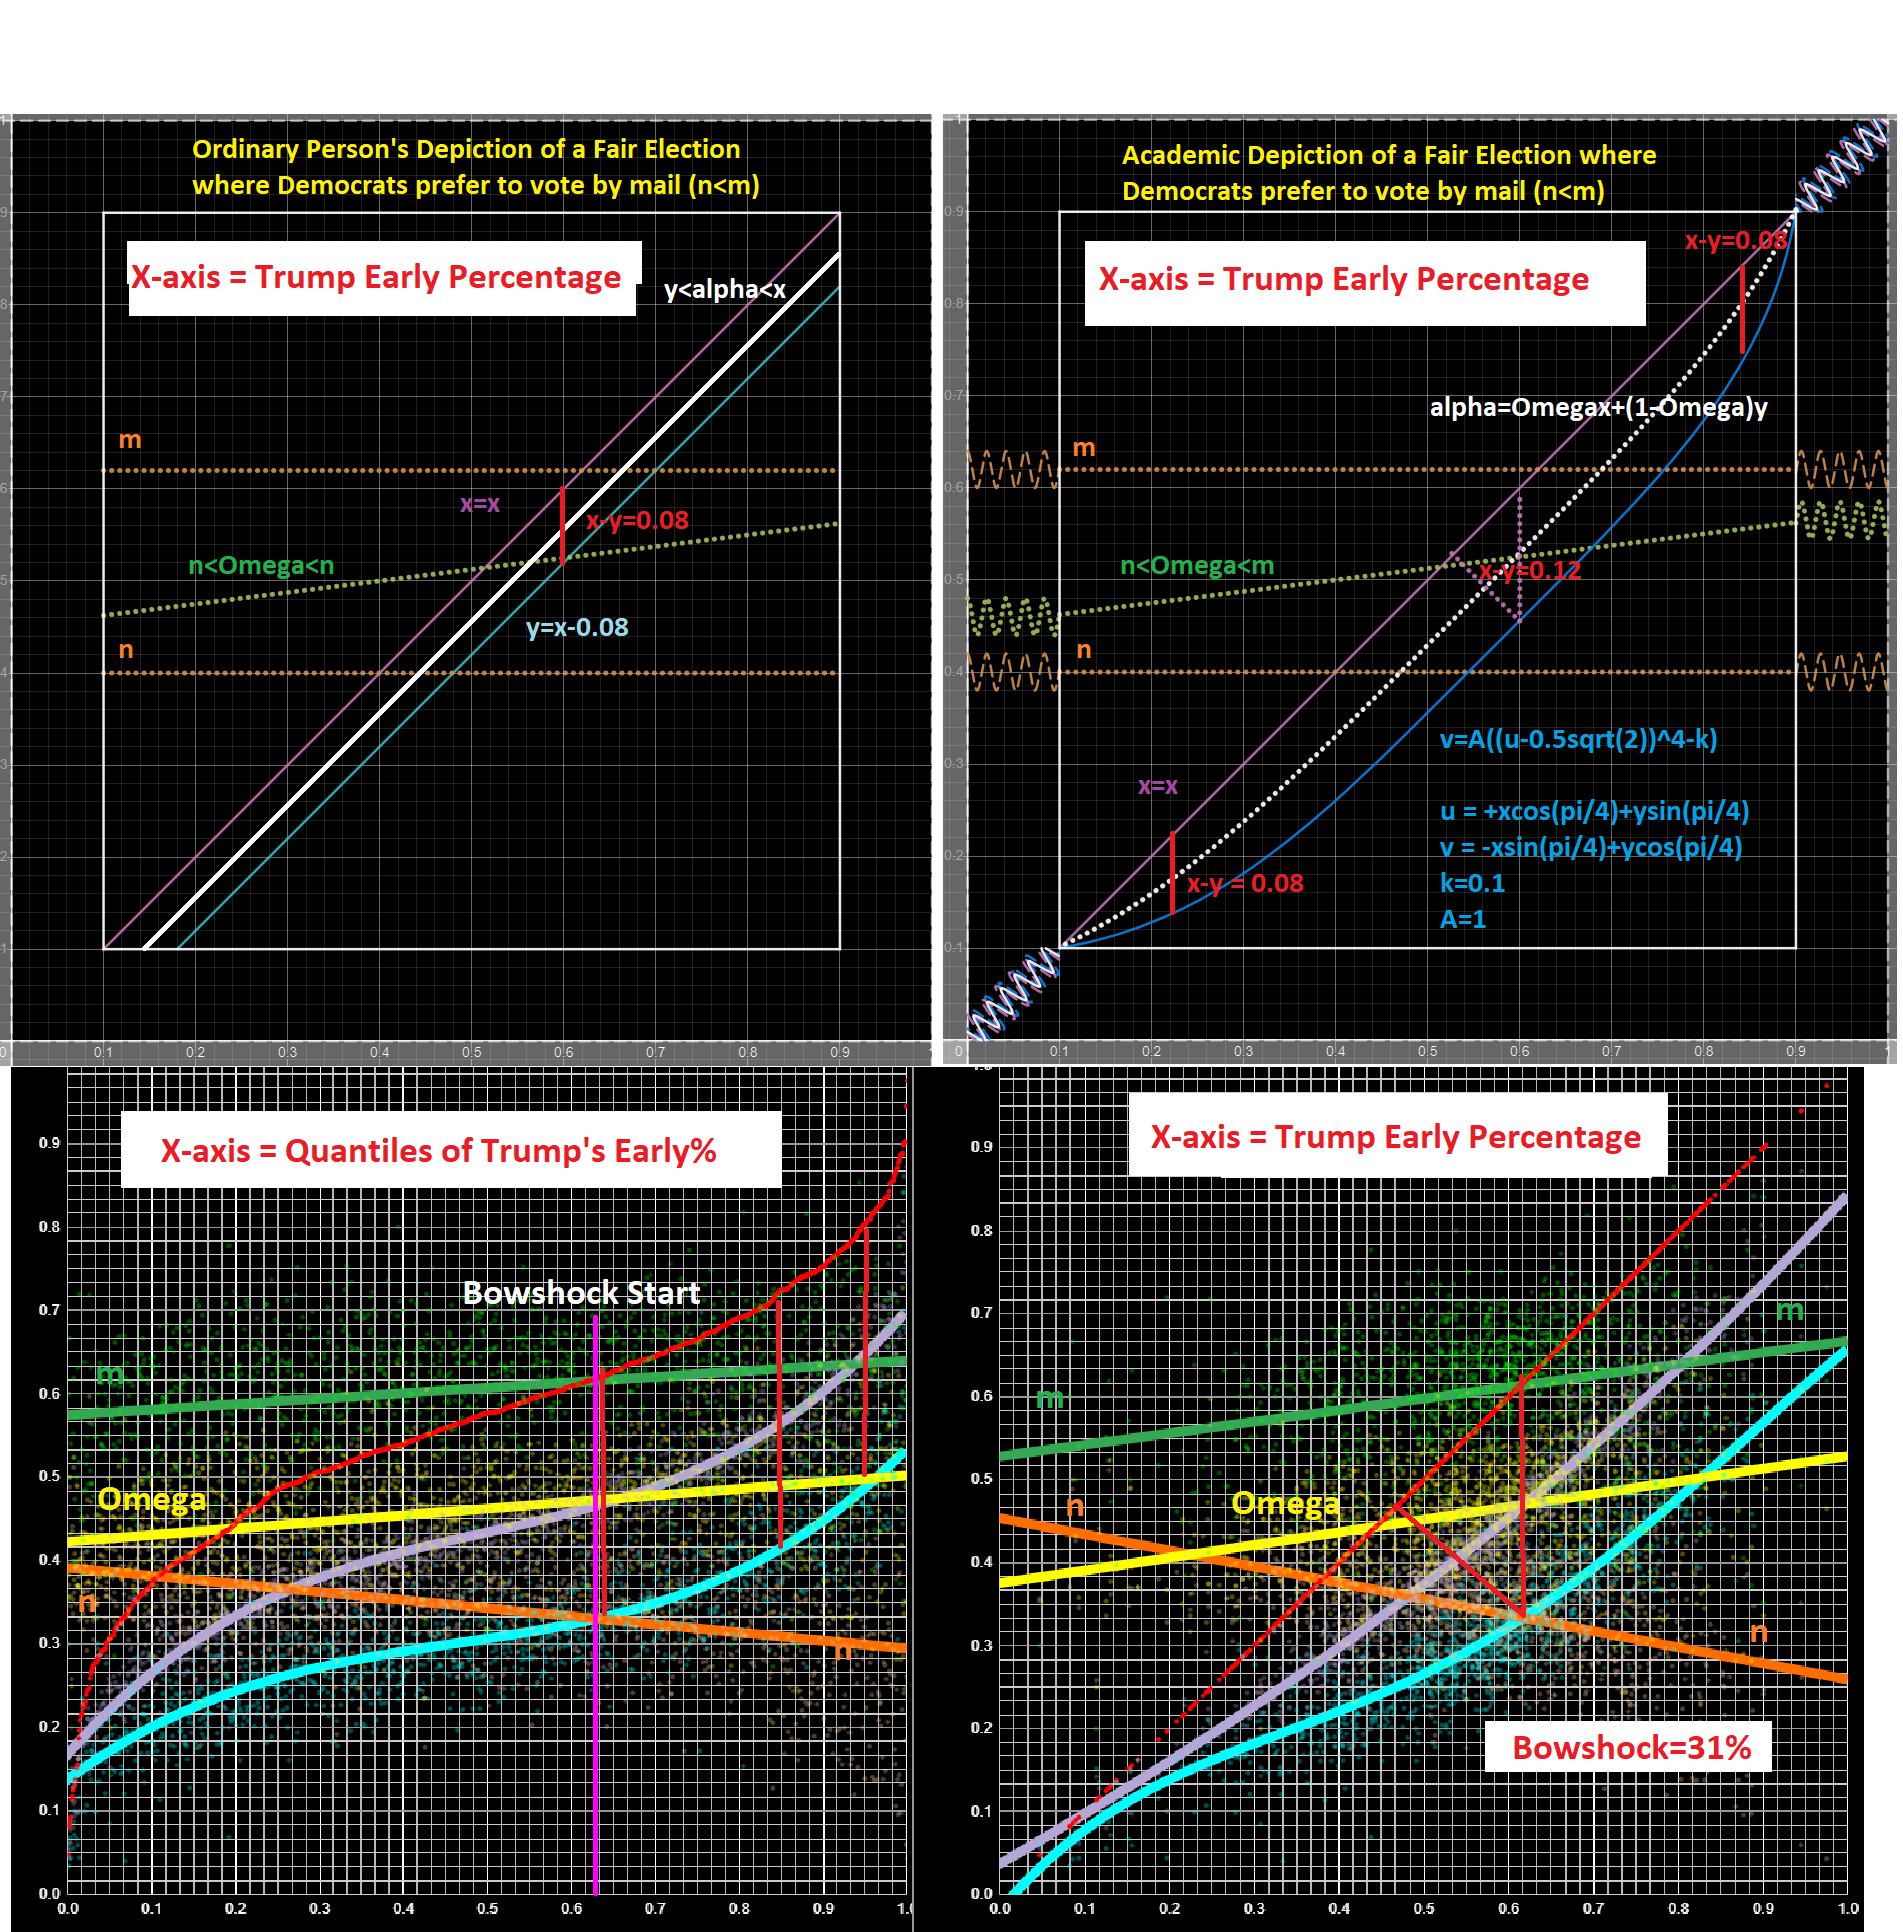
\includegraphics[width=300pt]{Clark County vs Common Sense.png}
\end{center}
\end{figure}
\newpage
\subsection{The Geometric Absurdity of Constant Lambda; Why the Defense Cannot Assert that Constant Lambda is not unusual in a Safe and Secure Election; And Why Lambda is Called the ``Obstacle Percentage"}

Usually by this point in the presentation to the common layman, where I've shown the $n$ decreases with $x$, that the distance between $x$ and $y$ diverges with $x$, that Biden's Mail-in Vote can be calculated knowing only the Total Ballots Cast and Trump's early Vote, and that $\alpha=0.635g+0.365h$, allowing you to calculate $\alpha$ in every precinct with no knowledge of $\lambda$ (violating the Fish Tank Paradox) in every precinct, the common lay person admits (and Bard and ChatGPT AI's) that it's a foregone conclusion that the Nevada election has been rigged.

However, for some reason, ``credentialed mathematicians" continue to protest and say (with no reasons given) that it there's nothing wrong with constant $\lambda$ across the precincts, even though they will readily admit that there would be something wrong with constant $\alpha$ or constant $\Omega$ across the precincts.

I finally say, ``Let us assume that Lambda is indeed constant across the precincts, and, as you said, there's nothing unusual about that, then you're saying that how Republicans perform in the Early Vote and how Republicans prefer to cast their ballots will \textbf{FORCE} how Democrats cast their ballots across the precinct."

You'd be surprised how many academics (who are majority left leaning) don't realize the gravity of the previous statement. They think I'm talking about statistical trends...but I'm not, I'm talking about geometry, I'm talking about the Twenty Laws and Forty Isometries.

You see, if one knows $\lambda_{1},x_{1}$  and $m_{1}$, then the remaining six percentages, $y_{1}, \alpha_{1}, \Omega_{1}, n_{1}, g_{1}$ and $h_{1}$ are also known, because their existence is \textbf{forced}. If one knows the proportion of $s$ to $u$, the proportion of $s$ to $t$ and the proportion of $(s+v)$ to $(s+v)+(u+t)$, then they know the proportions of all combinations of $s,t,u$ and $v$.

The Twenty Laws and Forty Isometries are just a collection of 60 general laws amongst a grand total of 1,008 Laws (equal to 2 times 9 times 8 Choose 3), that allow you to calculate any percentage (or its conserved partner) from any other three percentages of the remaining eight (whilst using the conserved values of the remaining eight percentages where needed to simply the equations).

The reason that I selected those particular Twenty Laws (and their respective Forty Isometries), is because they describe the immediate behavior between percentages confined to the same Orientation (North vs South, West vs East and Diagonal vs Diagonal)---but that doesn't mean there aren't other laws that (for instance), allow you to solve for $n$ or $y$ knowing $x$ and $m$ and $\lambda$, where $x$ and $m$ are quadrant pairing percentages from different Orientations.
\newpage
\begin{theorem}{The First Perversion Theorem, The Insanity of Constant Lambda and the Mail-in Percentage}

Given that:\\
$y_{1}=\frac{u}{u+v};y_{2}=1-y_{1}=\frac{v}{u+v}$

$y_{1}=\cos^{2}(\beta); y_{2}=\sin^{2}(\beta)$

$x_{1}=\frac{s}{s+t};x_{2}=1-x_{1}=\frac{t}{s+t}$

$x_{1}=\cos^{2}(\theta); x_{2}=\sin^{2}(\theta)$

$m_{1}=\frac{s}{s+u};m_{2}=1-m_{1}=\frac{u}{s+u}$

$m_{1}=\cos^{2}(\phi); m_{2}=\sin^{2}(\phi)$

$\lambda_{1}=\frac{s+v}{(s+v)+(u+t)};\lambda_{2}=1-\lambda_{1}=\frac{u+t}{(s+v)+(u+t)}$

$\lambda_{1}=\cos^{2}(\rho); \lambda_{2}=\sin^{2}(\rho)$

Then it follows that:
$$y_{1}=\frac{\lambda_{2}(m_{2}x_{1})}{\lambda_{1}m_{1}+x_{1}(m_{2}-m_{1})}$$

Proof:\\
$$\frac{s}{s+t}=\cos^{2}(\theta); \frac{t}{s+t}=\sin^{2}(\theta) \implies \frac{t}{s}=\tan^{2}(\theta) \implies t=s\tan^{2}(\theta)$$
$$\frac{s}{s+u}=\cos^{2}(\phi); \frac{u}{s+u}=\sin^{2}(\phi) \implies \frac{u}{s}=\tan^{2}(\phi) \implies u=s\tan^{2}(\phi)$$
$$\frac{s+v}{(s+v)+(u+t)}=\cos^{2}(\rho); \frac{u+t}{(s+v)+(u+t)}=\sin^{2}(\rho) \implies \frac{u+t}{s+v}=\tan^{2}(\rho)$$
$$(u+t)=(s+v)\tan^{2}(\rho) \implies v=\cot^{2}\rho(u+t-s\tan^{2}(\rho))$$
$$v=\cot^{2}\rho\left(s\tan^{2}(\phi)+s\tan^{2}(\theta)-s\tan^{2}(\rho)\right)=s\cot^{2}\rho\left(\tan^{2}(\phi)+\tan^{2}(\theta)-\tan^{2}(\rho)\right)$$
$$y_{1}=\frac{u}{u+v}=\frac{s\tan^{2}(\phi)}{s\tan^{2}(\phi)+s\cot^{2}\rho\left(\tan^{2}(\phi)+\tan^{2}(\theta)-\tan^{2}(\rho)\right)}$$
We now divide by s/s
$$y_{1}=\frac{u}{u+v}=\frac{\tan^{2}(\phi)}{\tan^{2}(\phi)+\cot^{2}\rho\left(\tan^{2}(\phi)+\tan^{2}(\theta)-\tan^{2}(\rho)\right)}$$
\newpage
We now simply the denominator of the fraction for $y_{1}$:
$$\tan^{2}(\phi)+\cot^{2}\rho\left(\tan^{2}(\phi)+\tan^{2}(\theta)-\tan^{2}(\rho)\right)=\tan^{2}(\phi)(1+\cot^{2}(\rho))+\tan^{2}(\theta)\cot^{2}(\rho)-1$$
We now substitute $(1+\cot^{2}(\rho))$ with $\csc^{2}(\rho)$:
$$\tan^{2}(\phi)(1+\cot^{2}(\rho))+\tan^{2}(\theta)\cot^{2}(\rho)-1=\tan^{2}(\phi)\csc^{2}(\rho)+\tan^{2}(\theta)\cot^{2}(\rho)-1$$
We now divide by the reciprocal of the $y_{1}$ denominator, $\tan^{2}(\phi)$, whose reciprocal is $\cot^{2}(\phi)$:
$$y_{1}=\frac{1}{\cot^{2}(\phi)\left(\tan^{2}(\theta)\cot^{2}(\rho)-1\right)+\csc^{2}(\rho)}$$
We temporarily solve for the reciprocal of $y_{1}$ to ease the calculations:
$$\frac{1}{y_{1}}=\cot^{2}(\phi)\left(\tan^{2}(\theta)\cot^{2}(\rho)-1\right)+\csc^{2}(\rho)$$
We now replace the trigonometric terms with their respective percentages. The trigonometric substitutions have served their purpose and are no longer needed.
$$\cot^{2}(\phi)\left(\tan^{2}(\theta)\cot^{2}(\rho)-1\right)+\csc^{2}(\rho)=\frac{m_{1}}{m_{2}}\left(\frac{x_{2}}{x_{1}}\frac{\lambda_{1}}{\lambda_{2}}-1 \right)+\frac{1}{\lambda_{2}}$$
$$\frac{m_{1}}{m_{2}}\left(\frac{x_{2}}{x_{1}}\frac{\lambda_{1}}{\lambda_{2}}-1 \right)+\frac{1}{\lambda_{2}}=\frac{m_{1}}{m_{2}}\left(\frac{\lambda_{1}x_{2}}{\lambda_{2}x_{1}}-1 \right)+\frac{1}{\lambda_{2}}$$
$$\frac{m_{1}}{m_{2}}\left(\frac{\lambda_{1}x_{2}}{\lambda_{2}x_{1}}-1 \right)+\frac{1}{\lambda_{2}}=\frac{m_{1}}{m_{2}}\left(\frac{\lambda_{1}x_{2}-\lambda_{2}x_{1}}{\lambda_{2}x_{1}} \right)+\frac{1}{\lambda_{2}}$$
$$\frac{m_{1}}{m_{2}}\left(\frac{\lambda_{1}x_{2}-\lambda_{2}x_{1}}{\lambda_{2}x_{1}} \right)+\frac{1}{\lambda_{2}}=\frac{m_{1}}{m_{2}}\left(\frac{\lambda_{1}(1-x_{1})-\lambda_{2}x_{1}}{\lambda_{2}x_{1}} \right)+\frac{1}{\lambda_{2}}$$
$$\frac{m_{1}}{m_{2}}\left(\frac{\lambda_{1}(1-x_{1})-\lambda_{2}x_{1}}{\lambda_{2}x_{1}} \right)+\frac{1}{\lambda_{2}}=\frac{m_{1}}{m_{2}}\left(\frac{\lambda_{1}-\lambda_{1}x_{1}-\lambda_{2}x_{1}}{\lambda_{2}x_{1}} \right)+\frac{1}{\lambda_{2}}$$
$$\frac{m_{1}}{m_{2}}\left(\frac{\lambda_{1}-\lambda_{1}x_{1}-\lambda_{2}x_{1}}{\lambda_{2}x_{1}} \right)+\frac{1}{\lambda_{2}}=\frac{m_{1}}{m_{2}}\left(\frac{\lambda_{1}-x_{1}(\lambda_{1}+\lambda_{2})}{\lambda_{2}x_{1}} \right)+\frac{1}{\lambda_{2}}$$

Since $\lambda_{1}+\lambda_{2}$ is equal to one, we simplify as:
$$\frac{m_{1}}{m_{2}}\left(\frac{\lambda_{1}-x_{1}(\lambda_{1}+\lambda_{2})}{\lambda_{2}x_{1}} \right)+\frac{1}{\lambda_{2}}=\frac{m_{1}}{m_{2}}\left(\frac{\lambda_{1}-x_{1}}{\lambda_{2}x_{1}} \right)+\frac{1}{\lambda_{2}}$$
\newpage
We continue by getting a common numerator and denominator:
$$\frac{m_{1}}{m_{2}}\left(\frac{\lambda_{1}-x_{1}}{\lambda_{2}x_{1}} \right)+\frac{1}{\lambda_{2}}=\frac{m_{1}(\lambda_{1}-x_{1})}{m_{2}\lambda_{2}x_{1}}+\frac{1}{\lambda_{2}}$$

We simplify again by unifying the entire expression over a single denominator:
$$\frac{m_{1}(\lambda_{1}-x_{1})}{m_{2}\lambda_{2}x_{1}}+\frac{1}{\lambda_{2}}=\frac{m_{1}(\lambda_{1}-x_{1})+m_{2}x_{1}}{m_{2}\lambda_{2}x_{1}}$$

We now write the full expansion of the numerator:
$$\frac{m_{1}(\lambda_{1}-x_{1})+m_{2}x_{1}}{m_{2}\lambda_{2}x_{1}}=\frac{m_{1}\lambda_{1}-m_{1}x_{1}+m_{2}x_{1}}{m_{2}\lambda_{2}x_{1}}$$

We now write the numerator in Mother Nature's Form:
$$\frac{m_{1}\lambda_{1}-m_{1}x_{1}+m_{2}x_{1}}{m_{2}\lambda_{2}x_{1}}=\frac{m_{1}\lambda_{1}+x_{1}(m_{2}-m_{1})}{m_{2}\lambda_{2}x_{1}}$$
Such that:
$$y_{1}=\frac{\lambda_{2}(m_{2}x_{1})}{\lambda_{1}m_{1}+x_{1}(m_{2}-m_{1})}$$

Which reads that, for elections, ``The Republican Mail-in Percentage is equal to the ratio of A to B, where:

A is the republican Election Day Percentage, $x_{1}$, scaled by the Conserved Value of the Republican Preference Percentage, $m_{2}$, both scaled by the East Vertical Aggregate, $\lambda_{2}$.

B is the sum of the Republican Preference Percentage, $m_{1}$, scaled by the West Vertical Aggregate, $\lambda_{1}$, and the Candidate's Election Day Percentage, $x_{1}$, scaled by the difference between the Conserved Value of the Republican Preference Percentage and the Republican Preference Percentage itself, $m_{2}-m_{1}$.

Therefore, if $\lambda_{1}$ is constant over the precincts (and thus $\lambda_{2}$ must also be constant over the precincts), with very little variation, it follows that how Republicans Perform on Election Day, $x_{1}$, and how Republicans Prefer To Cast their Ballots, $m_{1}$ and $m_{2}$, will \textbf{\textcolor{red}{FORCE}} the Ratio of Democrat Mail-in to Republican Mail-in Ballots, which is $\tan^{2}(\beta)$, and therefore force the mail-in percentage, $y_{1}$, which is equal to $\cos^{2}(\beta)$.
\begin{flushright}
\textbf{Q.E.D}
\end{flushright}
\end{theorem}
\newpage
\begin{theorem}{The Second Perversion Theorem, The Insanity of Constant Lambda and the Democrat Preference Percentage}

Given that:\\
$n_{1}=\frac{t}{t+v};n_{2}=1-n_{1}=\frac{v}{t+v}$

$n_{1}=\cos^{2}(\kappa); n_{2}=\sin^{2}(\kappa)$

$x_{1}=\frac{s}{s+t};x_{2}=1-x_{1}=\frac{t}{s+t}$

$x_{1}=\cos^{2}(\theta); x_{2}=\sin^{2}(\theta)$

$m_{1}=\frac{s}{s+u};m_{2}=1-m_{1}=\frac{u}{s+u}$

$m_{1}=\cos^{2}(\phi); m_{2}=\sin^{2}(\phi)$

$\lambda_{1}=\frac{s+v}{(s+v)+(u+t)};\lambda_{2}=1-\lambda_{1}=\frac{u+t}{(s+v)+(u+t)}$

$\lambda_{1}=\cos^{2}(\rho); \lambda_{2}=\sin^{2}(\rho)$

Then it follows that:
$$n_{1}=\frac{\lambda_{2}(x_{2}m_{1})}{\lambda_{1}x_{1}+m_{1}(x_{2}-x_{1})}$$

Proof:\\
$$\frac{s}{s+t}=\cos^{2}(\theta); \frac{t}{s+t}=\sin^{2}(\theta) \implies \frac{t}{s}=\tan^{2}(\theta) \implies t=s\tan^{2}(\theta)$$
$$\frac{s}{s+u}=\cos^{2}(\phi); \frac{u}{s+u}=\sin^{2}(\phi) \implies \frac{u}{s}=\tan^{2}(\phi) \implies u=s\tan^{2}(\phi)$$
$$\frac{s+v}{(s+v)+(u+t)}=\cos^{2}(\rho); \frac{u+t}{(s+v)+(u+t)}=\sin^{2}(\rho) \implies \frac{u+t}{s+v}=\tan^{2}(\rho)$$
$$(u+t)=(s+v)\tan^{2}(\rho) \implies v=\cot^{2}\rho(u+t-s\tan^{2}(\rho))$$
$$v=\cot^{2}\rho\left(s\tan^{2}(\phi)+s\tan^{2}(\theta)-s\tan^{2}(\rho)\right)=s\cot^{2}\rho\left(\tan^{2}(\phi)+\tan^{2}(\theta)-\tan^{2}(\rho)\right)$$
$$n_{1}=\frac{t}{t+v}=\frac{s\tan^{2}(\theta)}{s\tan^{2}(\theta)+s\cot^{2}\rho\left(\tan^{2}(\phi)+\tan^{2}(\theta)-\tan^{2}(\rho)\right)}$$
We now divide by s/s
$$n_{1}=\frac{t}{t+v}=\frac{\tan^{2}(\theta)}{\tan^{2}(\theta)+\cot^{2}\rho\left(\tan^{2}(\phi)+\tan^{2}(\theta)-\tan^{2}(\rho)\right)}$$
\newpage
We now simply the denominator of the fraction for $n_{1}$:
$$\tan^{2}(\theta)+\cot^{2}\rho\left(\tan^{2}(\phi)+\tan^{2}(\theta)-\tan^{2}(\rho)\right)=\tan^{2}(\theta)(1+\cot^{2}(\rho))+\tan^{2}(\phi)\cot^{2}(\rho)-1$$
We now substitute $(1+\cot^{2}(\rho))$ with $\csc^{2}(\rho)$:
$$\tan^{2}(\theta)(1+\cot^{2}(\rho))+\tan^{2}(\phi)\cot^{2}(\rho)-1=\tan^{2}(\theta)\csc^{2}(\rho)+\tan^{2}(\phi)\cot^{2}(\rho)-1$$
We now divide by the reciprocal of the $n_{1}$ denominator, $\tan^{2}(\theta)$, whose reciprocal is $\cot^{2}(\theta)$:
$$n_{1}=\frac{1}{\cot^{2}(\theta)\left(\tan^{2}(\phi)\cot^{2}(\rho)-1\right)+\csc^{2}(\rho)}$$
We temporarily solve for the reciprocal of $n_{1}$ to ease the calculations:
$$\frac{1}{n_{1}}=\cot^{2}(\theta)\left(\tan^{2}(\phi)\cot^{2}(\rho)-1\right)+\csc^{2}(\rho)$$
We now replace the trigonometric terms with their respective percentages. The trigonometric substitutions have served their purpose and are no longer needed.
$$\cot^{2}(\theta)\left(\tan^{2}(\phi)\cot^{2}(\rho)-1\right)+\csc^{2}(\rho)=\frac{x_{1}}{x_{2}}\left(\frac{m_{2}}{m_{1}}\frac{\lambda_{1}}{\lambda_{2}}-1 \right)+\frac{1}{\lambda_{2}}$$
$$\frac{x_{1}}{x_{2}}\left(\frac{m_{2}}{m_{1}}\frac{\lambda_{1}}{\lambda_{2}}-1 \right)+\frac{1}{\lambda_{2}}=\frac{x_{1}}{x_{2}}\left(\frac{\lambda_{1}m_{2}}{\lambda_{2}m_{1}}-1 \right)+\frac{1}{\lambda_{2}}$$
$$\frac{x_{1}}{x_{2}}\left(\frac{\lambda_{1}m_{2}}{\lambda_{2}m_{1}}-1 \right)+\frac{1}{\lambda_{2}}=\frac{x_{1}}{x_{2}}\left(\frac{\lambda_{1}m_{2}-\lambda_{2}m_{1}}{\lambda_{2}m_{1}} \right)+\frac{1}{\lambda_{2}}$$
$$\frac{x_{1}}{x_{2}}\left(\frac{\lambda_{1}m_{2}-\lambda_{2}m_{1}}{\lambda_{2}m_{1}} \right)+\frac{1}{\lambda_{2}}=\frac{x_{1}}{x_{2}}\left(\frac{\lambda_{1}(1-m_{1})-\lambda_{2}m_{1}}{\lambda_{2}m_{1}} \right)+\frac{1}{\lambda_{2}}$$
$$\frac{x_{1}}{x_{2}}\left(\frac{\lambda_{1}(1-m_{1})-\lambda_{2}m_{1}}{\lambda_{2}m_{1}} \right)+\frac{1}{\lambda_{2}}=\frac{x_{1}}{x_{2}}\left(\frac{\lambda_{1}-\lambda_{1}m_{1}-\lambda_{2}m_{1}}{\lambda_{2}m_{1}} \right)+\frac{1}{\lambda_{2}}$$
$$\frac{x_{1}}{x_{2}}\left(\frac{\lambda_{1}-\lambda_{1}m_{1}-\lambda_{2}m_{1}}{\lambda_{2}m_{1}} \right)+\frac{1}{\lambda_{2}}=\frac{x_{1}}{x_{2}}\left(\frac{\lambda_{1}-m_{1}(\lambda_{1}+\lambda_{2})}{\lambda_{2}m_{1}} \right)+\frac{1}{\lambda_{2}}$$

Since $\lambda_{1}+\lambda_{2}$ is equal to one, we simplify as:
$$\frac{x_{1}}{x_{2}}\left(\frac{\lambda_{1}-m_{1}(\lambda_{1}+\lambda_{2})}{\lambda_{2}m_{1}} \right)+\frac{1}{\lambda_{2}}=\frac{x_{1}}{x_{2}}\left(\frac{\lambda_{1}-m_{1}}{\lambda_{2}m_{1}} \right)+\frac{1}{\lambda_{2}}$$
\newpage
We continue by getting a common numerator and denominator:
$$\frac{x_{1}}{x_{2}}\left(\frac{\lambda_{1}-m_{1}}{\lambda_{2}m_{1}} \right)+\frac{1}{\lambda_{2}}=\frac{x_{1}(\lambda_{1}-m_{1})}{x_{2}\lambda_{2}m_{1}}+\frac{1}{\lambda_{2}}$$

We simplify again by unifying the entire expression over a single denominator:
$$\frac{x_{1}(\lambda_{1}-m_{1})}{x_{2}\lambda_{2}m_{1}}+\frac{1}{\lambda_{2}}=\frac{x_{1}(\lambda_{1}-m_{1})+x_{2}m_{1}}{x_{2}\lambda_{2}m_{1}}$$

We now write the full expansion of the numerator:
$$\frac{x_{1}(\lambda_{1}-m_{1})+x_{2}m_{1}}{x_{2}\lambda_{2}m_{1}}=\frac{x_{1}\lambda_{1}-x_{1}m_{1}+x_{2}m_{1}}{x_{2}\lambda_{2}m_{1}}$$

We now write the numerator in Mother Nature's Form:
$$\frac{x_{1}\lambda_{1}-x_{1}m_{1}+x_{2}m_{1}}{x_{2}\lambda_{2}m_{1}}=\frac{x_{1}\lambda_{1}+m_{1}(x_{2}-x_{1})}{x_{2}\lambda_{2}m_{1}}$$
Such that:
$$n_{1}=\frac{\lambda_{2}(x_{2}m_{1})}{\lambda_{1}x_{1}+m_{1}(x_{2}-x_{1})}$$

Which reads that, for elections, ``The Percentage of Democrats that shall Prefer to Vote on Election Day, instead of by Mail, is equal to the Proportion of C to D, where:

C is the Democrat's Election Day Percentage, $x_{2}$, scaled by the Republican's Preference Percentage, $m_{1}$, both scaled by the East Vertical Aggregate, $\lambda_{2}$.

D is the sum of the Republican Election Day Percentage, $x_{1}$, scaled by the West Vertical Aggregate, $\lambda_{1}$, and the Republican Preference Percentage, $m_{1}$, scaled by the difference between the Conserved Values of the Democrat and Republican Election Day Percentages, $x_{2}-x_{1}$.

Therefore, if $\lambda_{1}$ is constant over the precincts (and therefore $\lambda_{2}$ is also constant over the precincts), with very little variation, it follows that how Republicans Prefer to Cast their ballots, $m_{1}$, and how Republicans and Democrats choose to vote on Election Day, $x_{1}$ and $x_{2}$, will \textbf{\textcolor{red}{FORCE}} the Ratio of Democrat Mail-in to Democrat Election Day Ballots, which is $\tan^{2}(\kappa)$, and therefore force the Democrat Preference Percentage, $n_{1}$, which is equal to $\cos^{2}(\kappa)$.
\begin{flushright}
\textbf{Q.E.D}
\end{flushright}
\end{theorem}
\newpage
\begin{theorem}{The Third Perversion Theorem, The Insanity of Lambda being Parallel to M}

If the trajectories of $\lambda$ and $m$ are parallel over the quantiles of $x$, such that the difference between the trajectories of $\lambda$ and $m$ is $k$, where $k=\lambda-m$, then:

$$y_{1}=\frac{\lambda_{2}(m_{2}x_{1})}{\lambda_{1}m_{1}+x_{1}(m_{2}-m_{1})}=\frac{(1-\lambda_{1})(1-m_{1})x_{1}}{\lambda_{1}m_{1}+x_{1}(1-2m_{1})}$$

$$y_{1}=\frac{(\lambda_{1}^2-\lambda_{1}(2+k)+k+1)x_{1}}{\lambda_{1}^2-\lambda_{1}k+x_{1}(1+2k-2\lambda_{1})}$$
\end{theorem}
In the below figure is the manifold for $k=0.03$, the grey vertical plane is $\lambda_{1}=0.573+0.11x$, which is the trajectory of $\lambda$ in respect to x. 

The intersection of the vertical grey plane and the pink manifold for $k=0.03$ is the resultant mail-in percentage, which compared against the diagonal plane $y=x$ so you can observe the \textbf{FORCED} bowshock (forced divergence of the distance between the Early and Mail-in Percentages). 

This general pattern persists over the entire range for $k$ from -1 to 1. \textcolor{red}{Thus, the Republicans will always suffer in the Mail-in Vote the better they perform on Election Day (or Early)} when the trajectory of $m$ is parallel to $\lambda$.
\begin{figure}[bp!]
\begin{center}
\caption{The Manifold of M Parallel to Lambda}
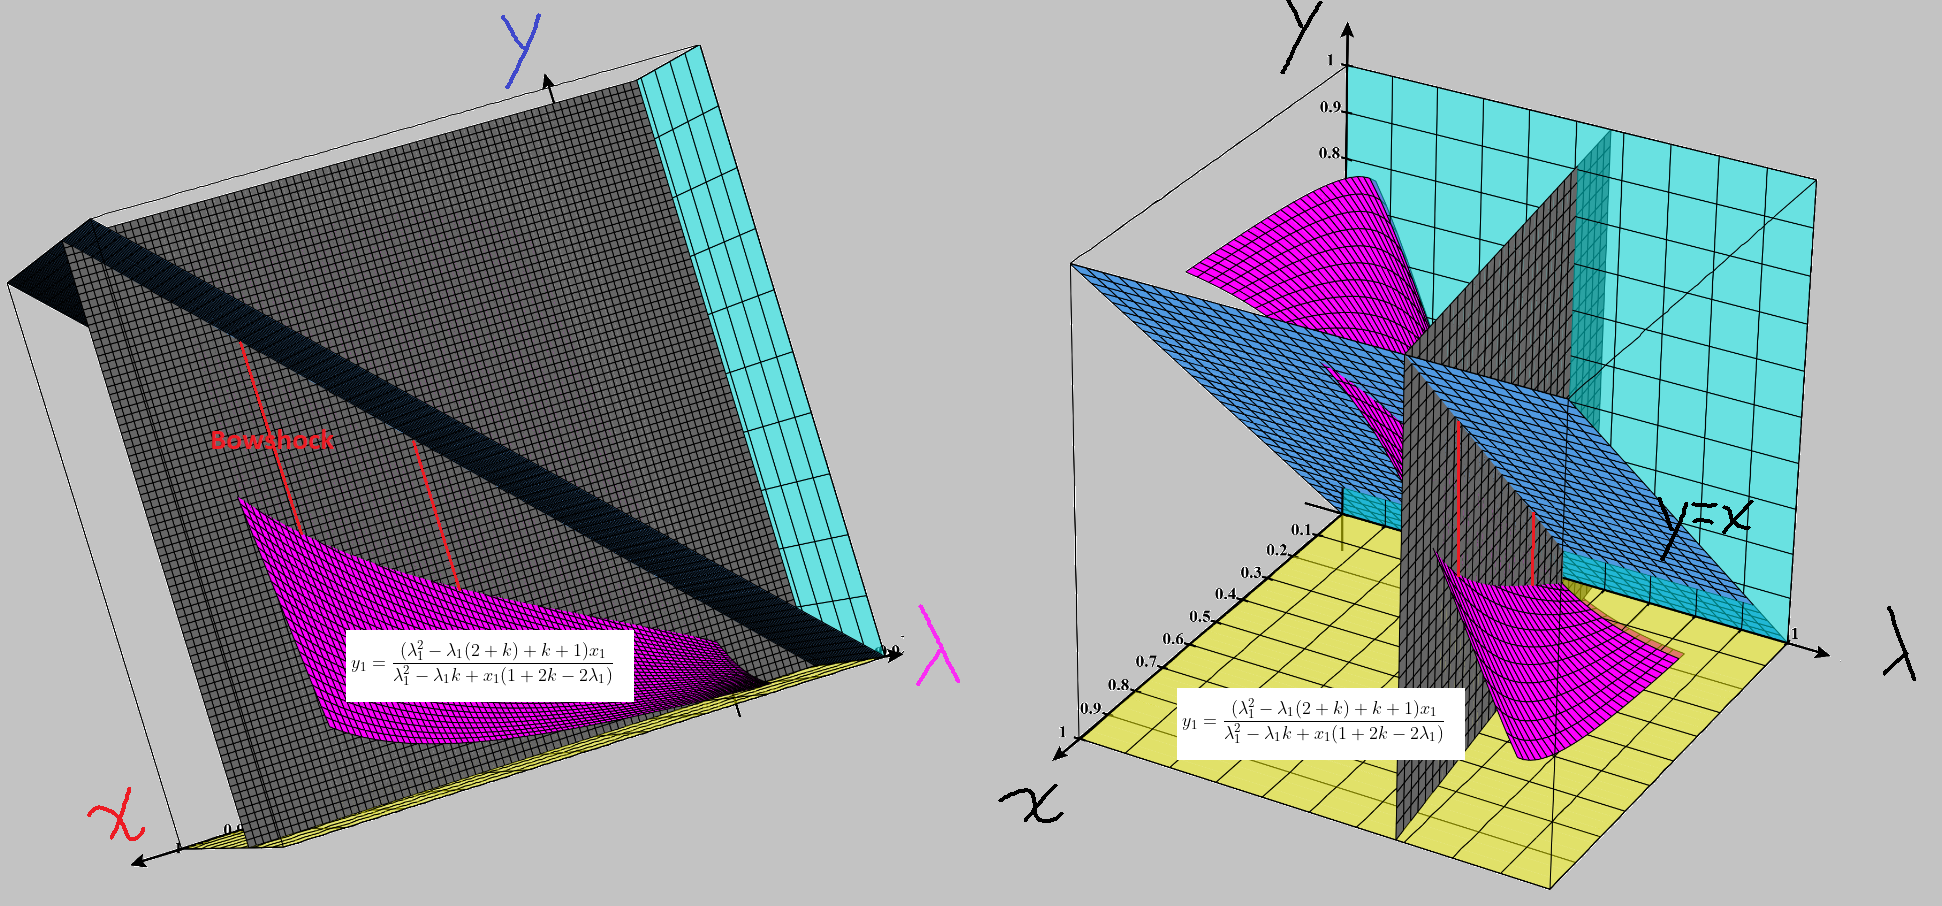
\includegraphics[width=400pt]{Parallel Lambda M parametric.png}
\end{center}
\end{figure}
\newpage
Below are precincts sorted by Trump's Early Percentage, $x$, where the horizontal axis are the Quantiles of $x$. The pink and orange trajectories are the trajectories of $\lambda$ and $m$ respectively over the quantiles of $x$, you can see the forced result for $y$ and $n$ (the Republican Mail-in Percentage and the Democrat Preference Percentage, respectively).

Remember that the manifold of $y_{1}=\frac{(\lambda_{1}^2-\lambda_{1}(2+k)+k+1)x_{1}}{\lambda_{1}^2-\lambda_{1}k+x_{1}(1+2k-2\lambda_{1})}$ doesn't care whether or not the horizontal axis is $x$ itself or the quantiles of $x$, thus no matter what happens, as $x$ increases, more Democrats will prefer to vote by mail at an alarming rate and the distance between $x$ and $y$ must diverge.
\begin{figure}[bp!]
\begin{center}
\caption{M Parallel to Lambda Over the Quantiles of X, Nevada 2020}
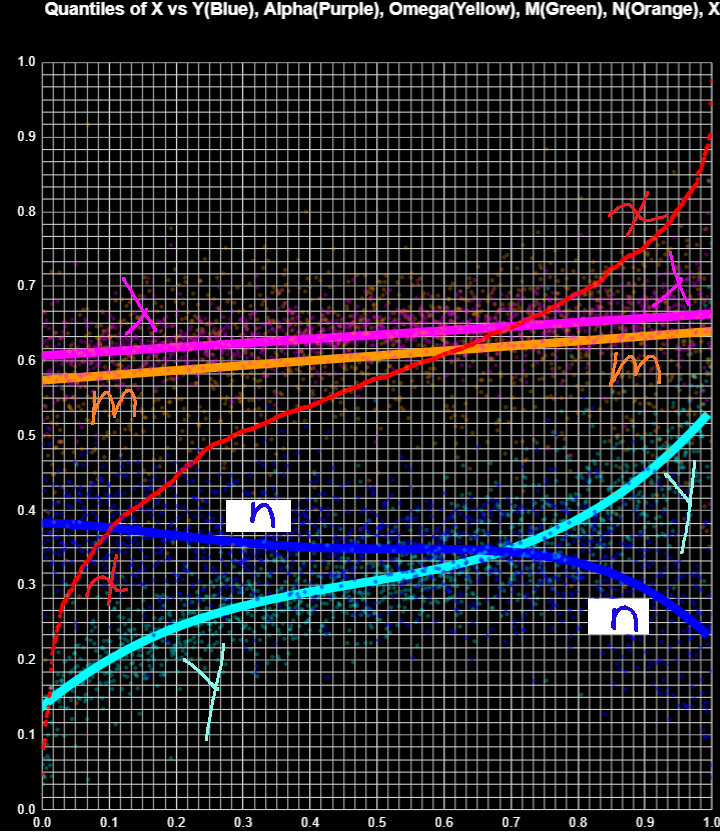
\includegraphics[width=300pt]{M Lambda Parallel.png}
\end{center}
\end{figure}
\newpage
You may be surprised that \textbf{some} academics up to this point in presentation (article), will still continue to resist. They will claim that perhaps the election day percentage (or the early percentage), $x_{1}$, is not the proper description of the election (meaning the horizontal axis shouldn't be $x_{1}$ or the quantiles of $x_{1}$), and will then discard the previous three Perversion Theorems and spout some Main Stream Media nonsense of how Democrats prefer to vote by mail.

After they're done saying whatever it is they want to say (which they cannot even put in concrete mathematical terms, and refuse to put in concrete mathematical terms) , I then show the the $46^{th}$ Isometry, which is the Diagonal vs Diagonal Isometry of the $6^{th}$ Law, which itself is the Hyperbolic Reflection Theorem.

The power of the $46^{th}$ Isometry is that it \textbf{temporarily concedes} the argument that either the $x$ and/or $y$ percentages are not the proper description of the election, thus we use $\alpha$ to describe the election...after all, no one, including these academics, can disagree that $\alpha$ properly describes the election---for the winner of an election is determined by $\alpha$. (one of my friends joked ``If Emperor Palpatine was the Alpha Percentage, he would exclaim `I am the Election!'")

\begin{theorem}{The Fourth Perversion Theorem, The Alpha Reflection Theorem}
$$n_{1}=\lambda_{2}-\xi^{-1}(\lambda_1-m_{1})=\lambda_{2}-\frac{\alpha_{1}}{\alpha_{2}}(\lambda_1-m_{1}) \implies n_{2}=\lambda_{1}+\frac{\alpha_{1}}{\alpha_{2}}(\lambda_1-m_{1})$$

This states that the percentage of Democrats that prefer to vote by mail, $n_2$, as opposed to Early (remember that $n_{2}=\frac{Democrat Mail}{Democrat Early+Democrat Mail}$), is the reflection of $m_{1}$, which is the percentage of Republicans that prefer to vote Early, over the line of $\lambda$, scaled by proportion of total Republican to total Democrat ballots.

Thus if $m_{1}$ is parallel to $\lambda_{1}$ in respect to $\alpha_{1}$ or the quantiles of $\alpha_{1}$,  that $n_{2}>m_{1}$ and the $n_{2}$ must increase exponentially, the better than Republicans perform overall, $\alpha_{1}$. Furthermore the more Republicans that prefer to vote early (as $m_{1}$ increases, and therefore $\lambda_{1}$ also increases since they are parallel), the more Democrats \textbf{ARE FORCED} to vote by mail.
\end{theorem}
Thus after the academics are done digging their graves about Republican Early/Election Day turnout being higher in Republican precincts (increasing $m_{1}$), I then show them that it translates to, directly, increased Democrat turnout by mail in those very same high performing Republican precincts.
\newpage
In the below graphs, as $\alpha_{1}$ increases (the white line), that if $m_{1}$ (which is the percentage of Republicans that prefer to vote Early, instead of by mail) is parallel to $\lambda_{1}$, that $n_{2}$, which is the percentage of Democrats that prefer to vote by Mail, as opposed to Early, cannot be less than $\lambda_{1}$, and thus must always be greater than $m_{1}$, because $n_{2}$ is the reflection of $m_{1}$ over $\lambda_{1}$.

This also means that the more energy there is in the Republican electorate (the more they turnout to vote on election day or early at precinct), the more energy there is in the Democrat electorate to turn out by mail in Republican precincts. You can see this in the bottom two graphs (bottom left and bottom center), where I put $m_{1}$ and $\lambda_{1}$ on positive incline in respect to $\alpha_{1}$, which forces $n_{2}$ to explode (bottom center), and the distance between $x_{1}$ and $y_{1}$ (which are the Early and Mail-in Percentages for the Republicans) to diverge within the range of $0 \le \alpha_{1} \le 0.7$, creating a massive bowshock!

You can go to this link and adjust the slope of $m_{1}$ and $\lambda_{1}$ via the $w$ operator and the difference between via the $k$ operator and starting value of $\lambda_{1}$ at $\alpha_{1}=0$ via the $z$ operator.
\url{https://www.desmos.com/calculator/p3iely2hhx}
\begin{figure}[bp!]
\begin{center}
\caption{M Parallel to Lambda Over the Quantiles of X, Nevada 2020}
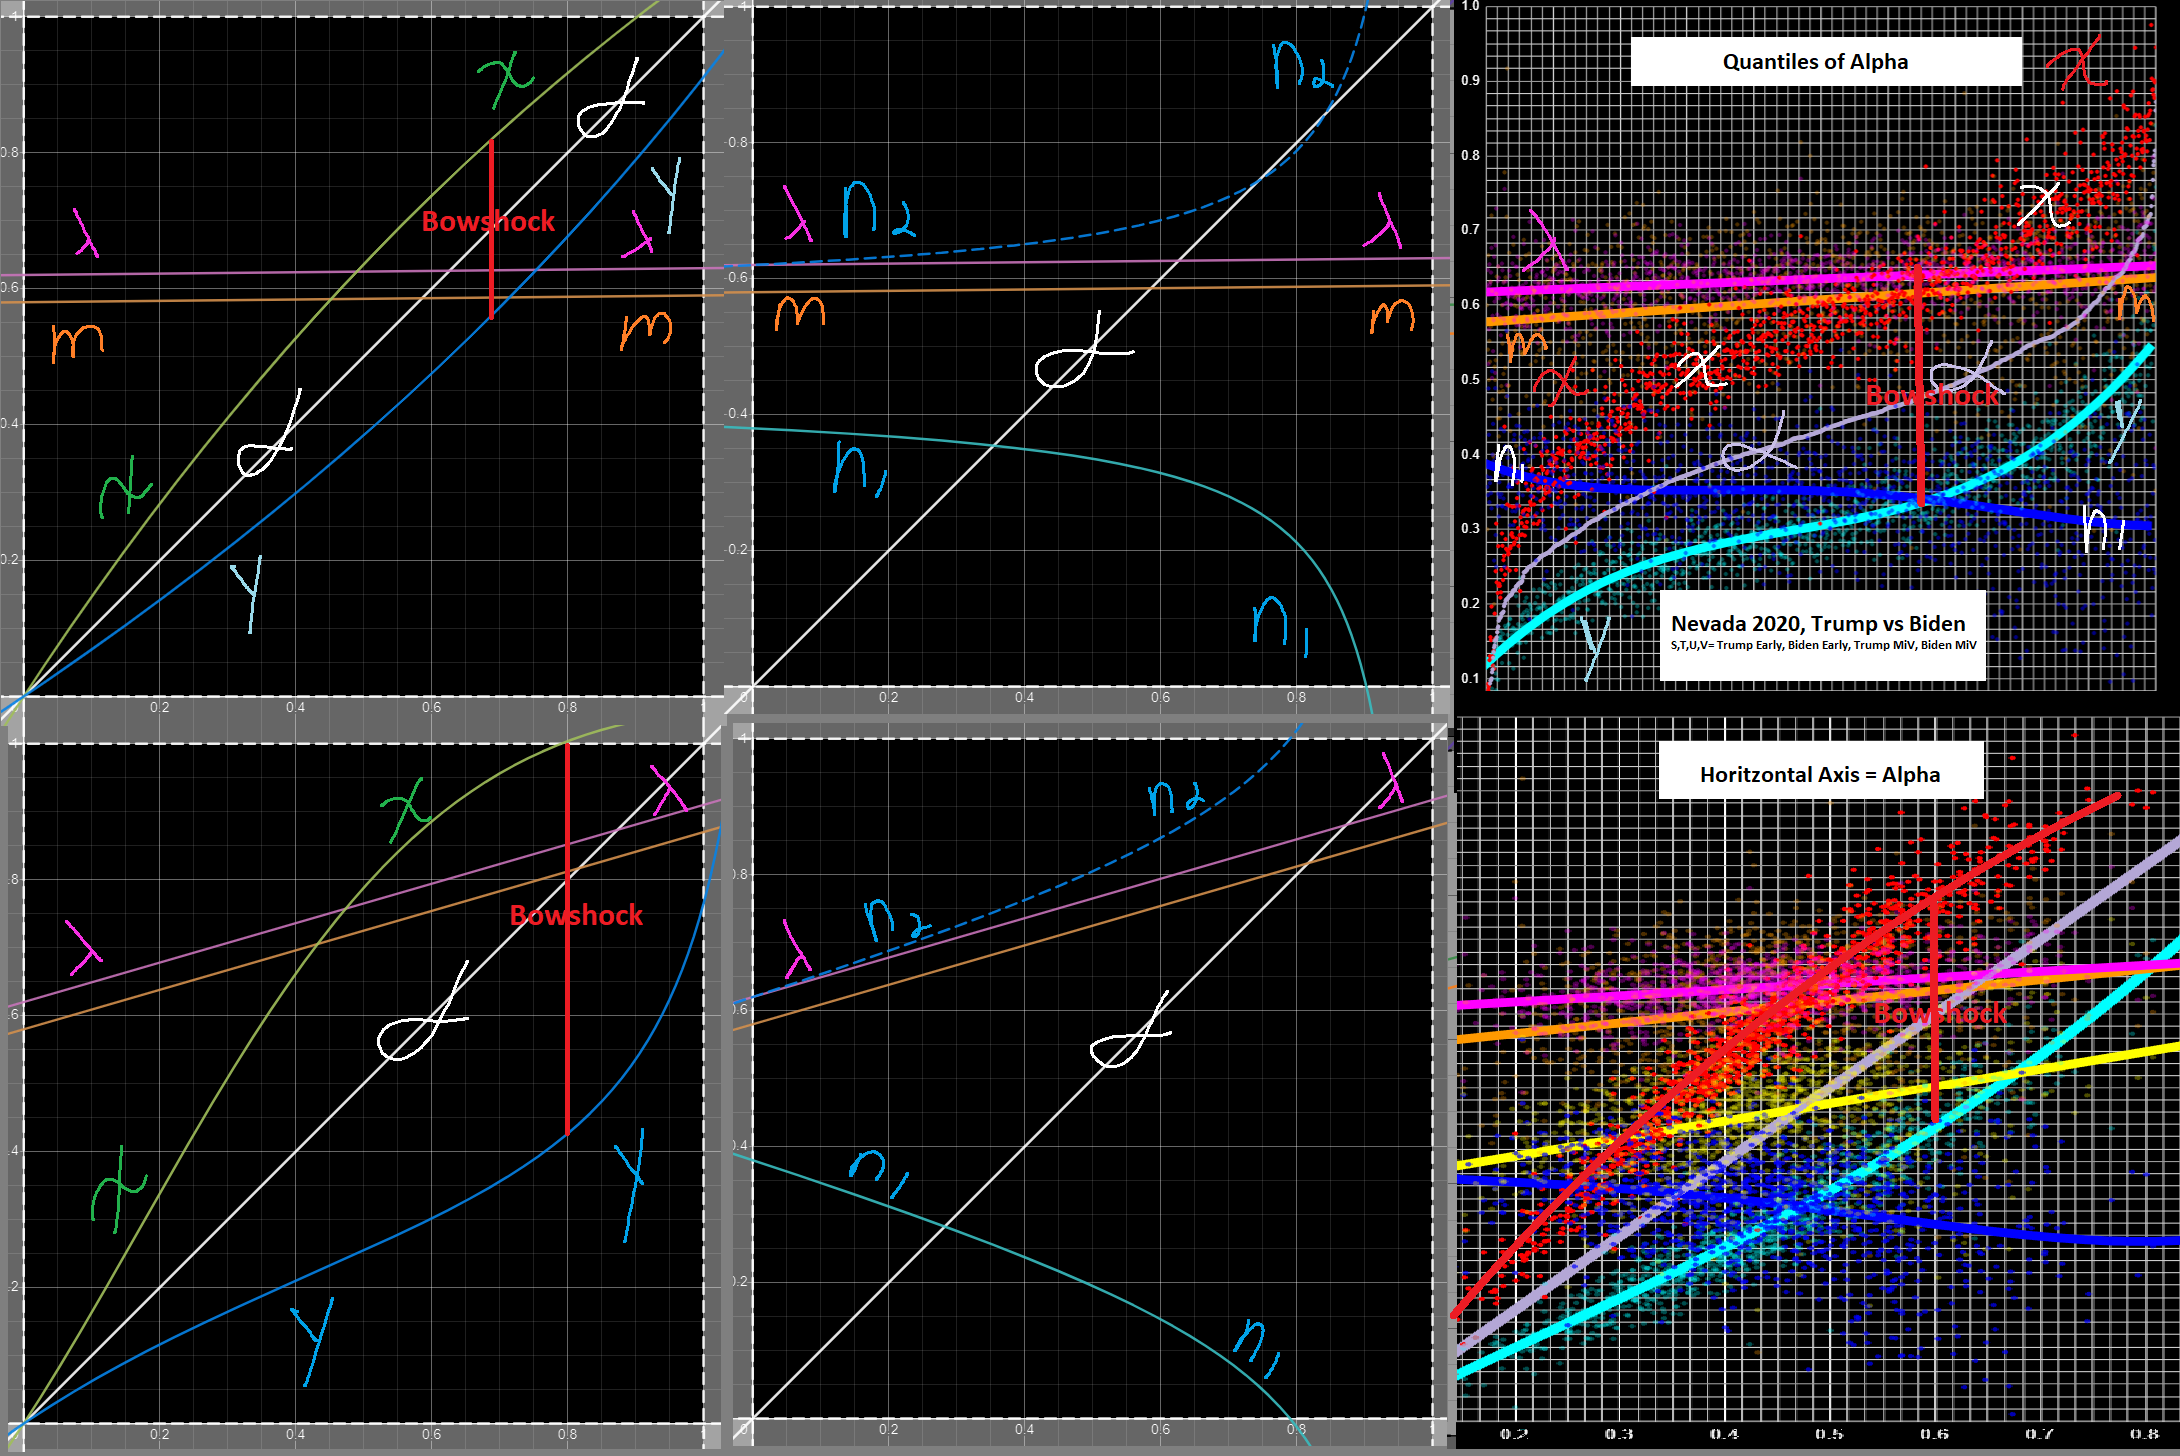
\includegraphics[width=400pt]{Alpha Reflection Theorem, Nevada 2020.png}
\end{center}
\end{figure}
\newpage
After showing an academic the ``Alpha Reflection," you would think they would finally concede. Each time they've moved the goalposts (such as using $\alpha$ instead of $x$ to describe the election), I've struck them down using pure geometry...but alas, they have one last ``trick up their sleeve" in an attempt to deny the absurdity of $m$ and $n$ diverging.

They (the few academics who continue resisting) will each independently (since I talk to them in isolation) show me the below graph (top-left) of $m$ increasing with $n$. They will then proclaim that that I am wrong and that the Democrat $n$ does not decrease with the Republican $m$, yet all they are doing is show me an orthogonal projection \textbf{(an optical illusion---a lie)} of the $m,n,\alpha$ coordinates onto the $m,n$ plane.

You see the Ninth Law, via the $49^{th}$ Isometry, states the that $m$, $n$ and $\alpha$ can all exist independently from 0\% to 100\%, viz. $\Omega=m\alpha+(1-\alpha)n$. Thus showing us the top-left graph doesn't tell us anything about the election, because $m$ and $n$ alone don't resolve the proportions of $s$ to $t$ to $u$ to $v$...and they know that. The most it tells us is the boundaries of $\Omega$, since $\Omega$ must exist between $m$ and $n$, which places \textbf{wide boundaries} on $x,y,g,h,\alpha$ and $\lambda$.

To make a long story short, knowledge of $m$ and $n$ is meaningless without knowledge of $\alpha$...and they know that. Because if they don't know that, they shouldn't have a math degree---thus they are intentionally obfuscating in an attempt to deceive us; hence why I called it a ``trick up their sleeve."
\begin{figure}[bp!]
\begin{center}
\caption{The Deceiver vs the Layman, Nevada 2020}
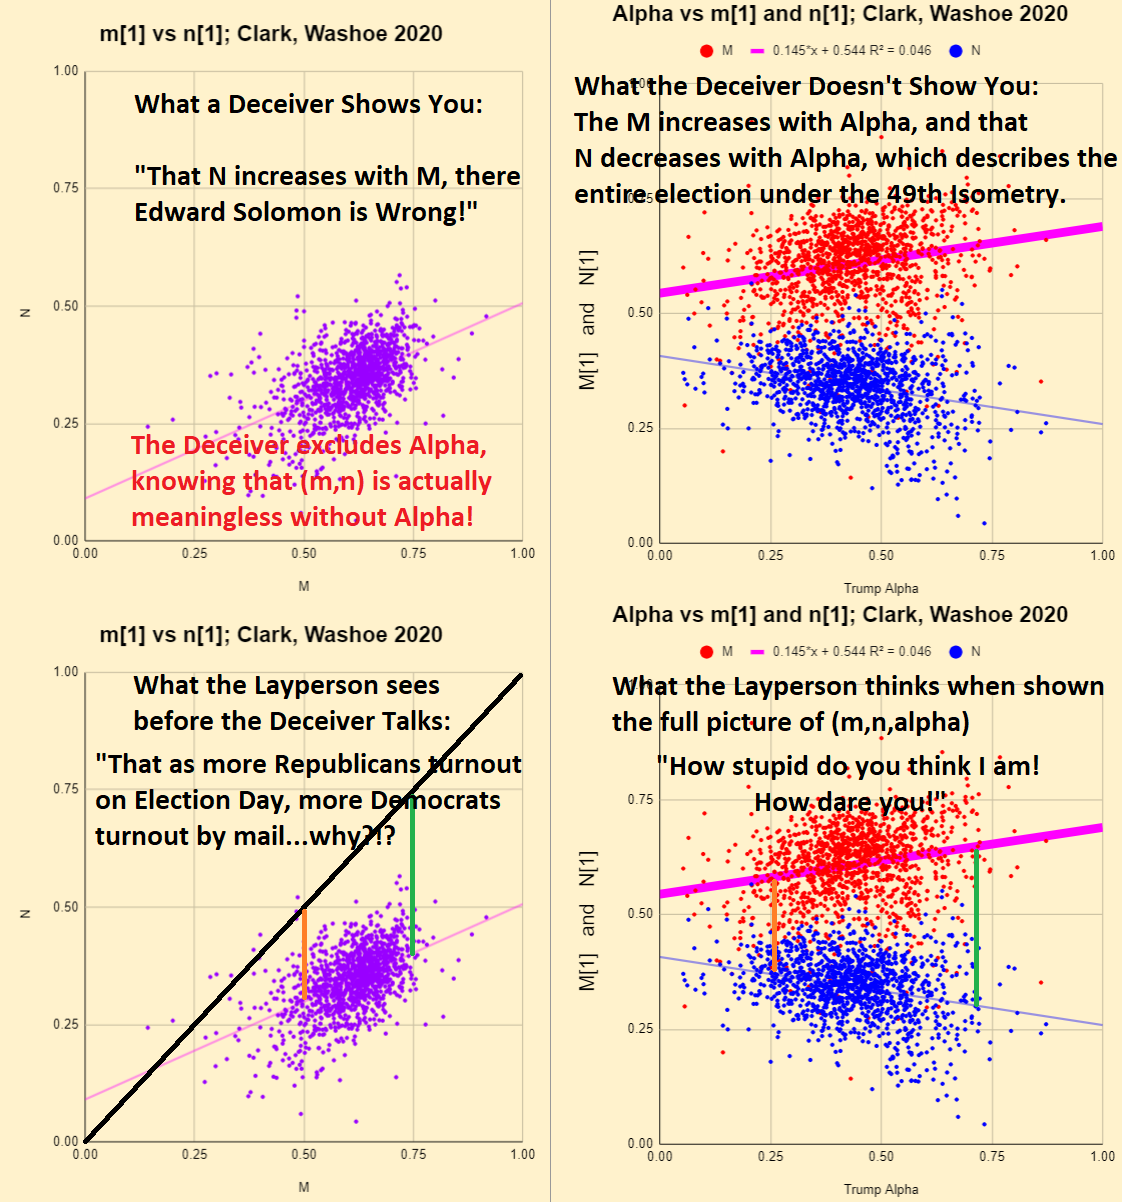
\includegraphics[width=200pt]{MvsN Clark.png}
\end{center}
\end{figure}
\newpage
\newpage
In the top-left and top-right graphs show the same (nearly flat) trajectory for $\lambda_{1}$ (in orange) in respect to the Early Percentage (or election day percentage), $x_{1}$.

The Sixth Law prevents the Democrat's mail-in percentage, $y_{2}$, from falling below $\lambda_{1}$, until the Republican Early Percentage exceeds $\lambda_{1}$, since $y_{2}$ is the reflection of $x_{1}$ over the line of $\lambda_{1}$, scaled by $\frac{\Omega_{1}}{\Omega_{2}}$, regardless of the value $\Omega_{1}$ (notice the trajectories of $\Omega_{1}$ are different in the top-left and top-right graphs, yet the Democrat Mail-in Percentage cannot fall below $\lambda_{1}$ until $x_{1}=\lambda_{1}$).

In the bottom-left and bottom-right graphs I placed the trajectory of $\lambda_{1}$ on a higher incline, while using the same two trajectories for $\Omega_{1}$ from the top-left and top-right graphs, respectively. Notice again that regardless of the value of $\Omega_{1}$, that the Democrat Mail-in Percentage, $y_{2}$ cannot fall below $\lambda_{1}$ until $x_{1}$ exceeds $\lambda_{1}$. 

Also, observe the Bowshocks (the maximum distance between $x_{1}$ and the trajectory of $y_{1}$) in each of the four graphs, in the bottom-right graph, the Bowshock can't even be realized since it occurs when $x>100\%$. You can interact with these graphs here: \url{https://www.desmos.com/calculator/uci7sw10dk}
\begin{figure}[bp!]
\begin{center}
\caption{The Sixth Law: The Democrat's Mail-in Percentage vs X, Omega and Lambda.}
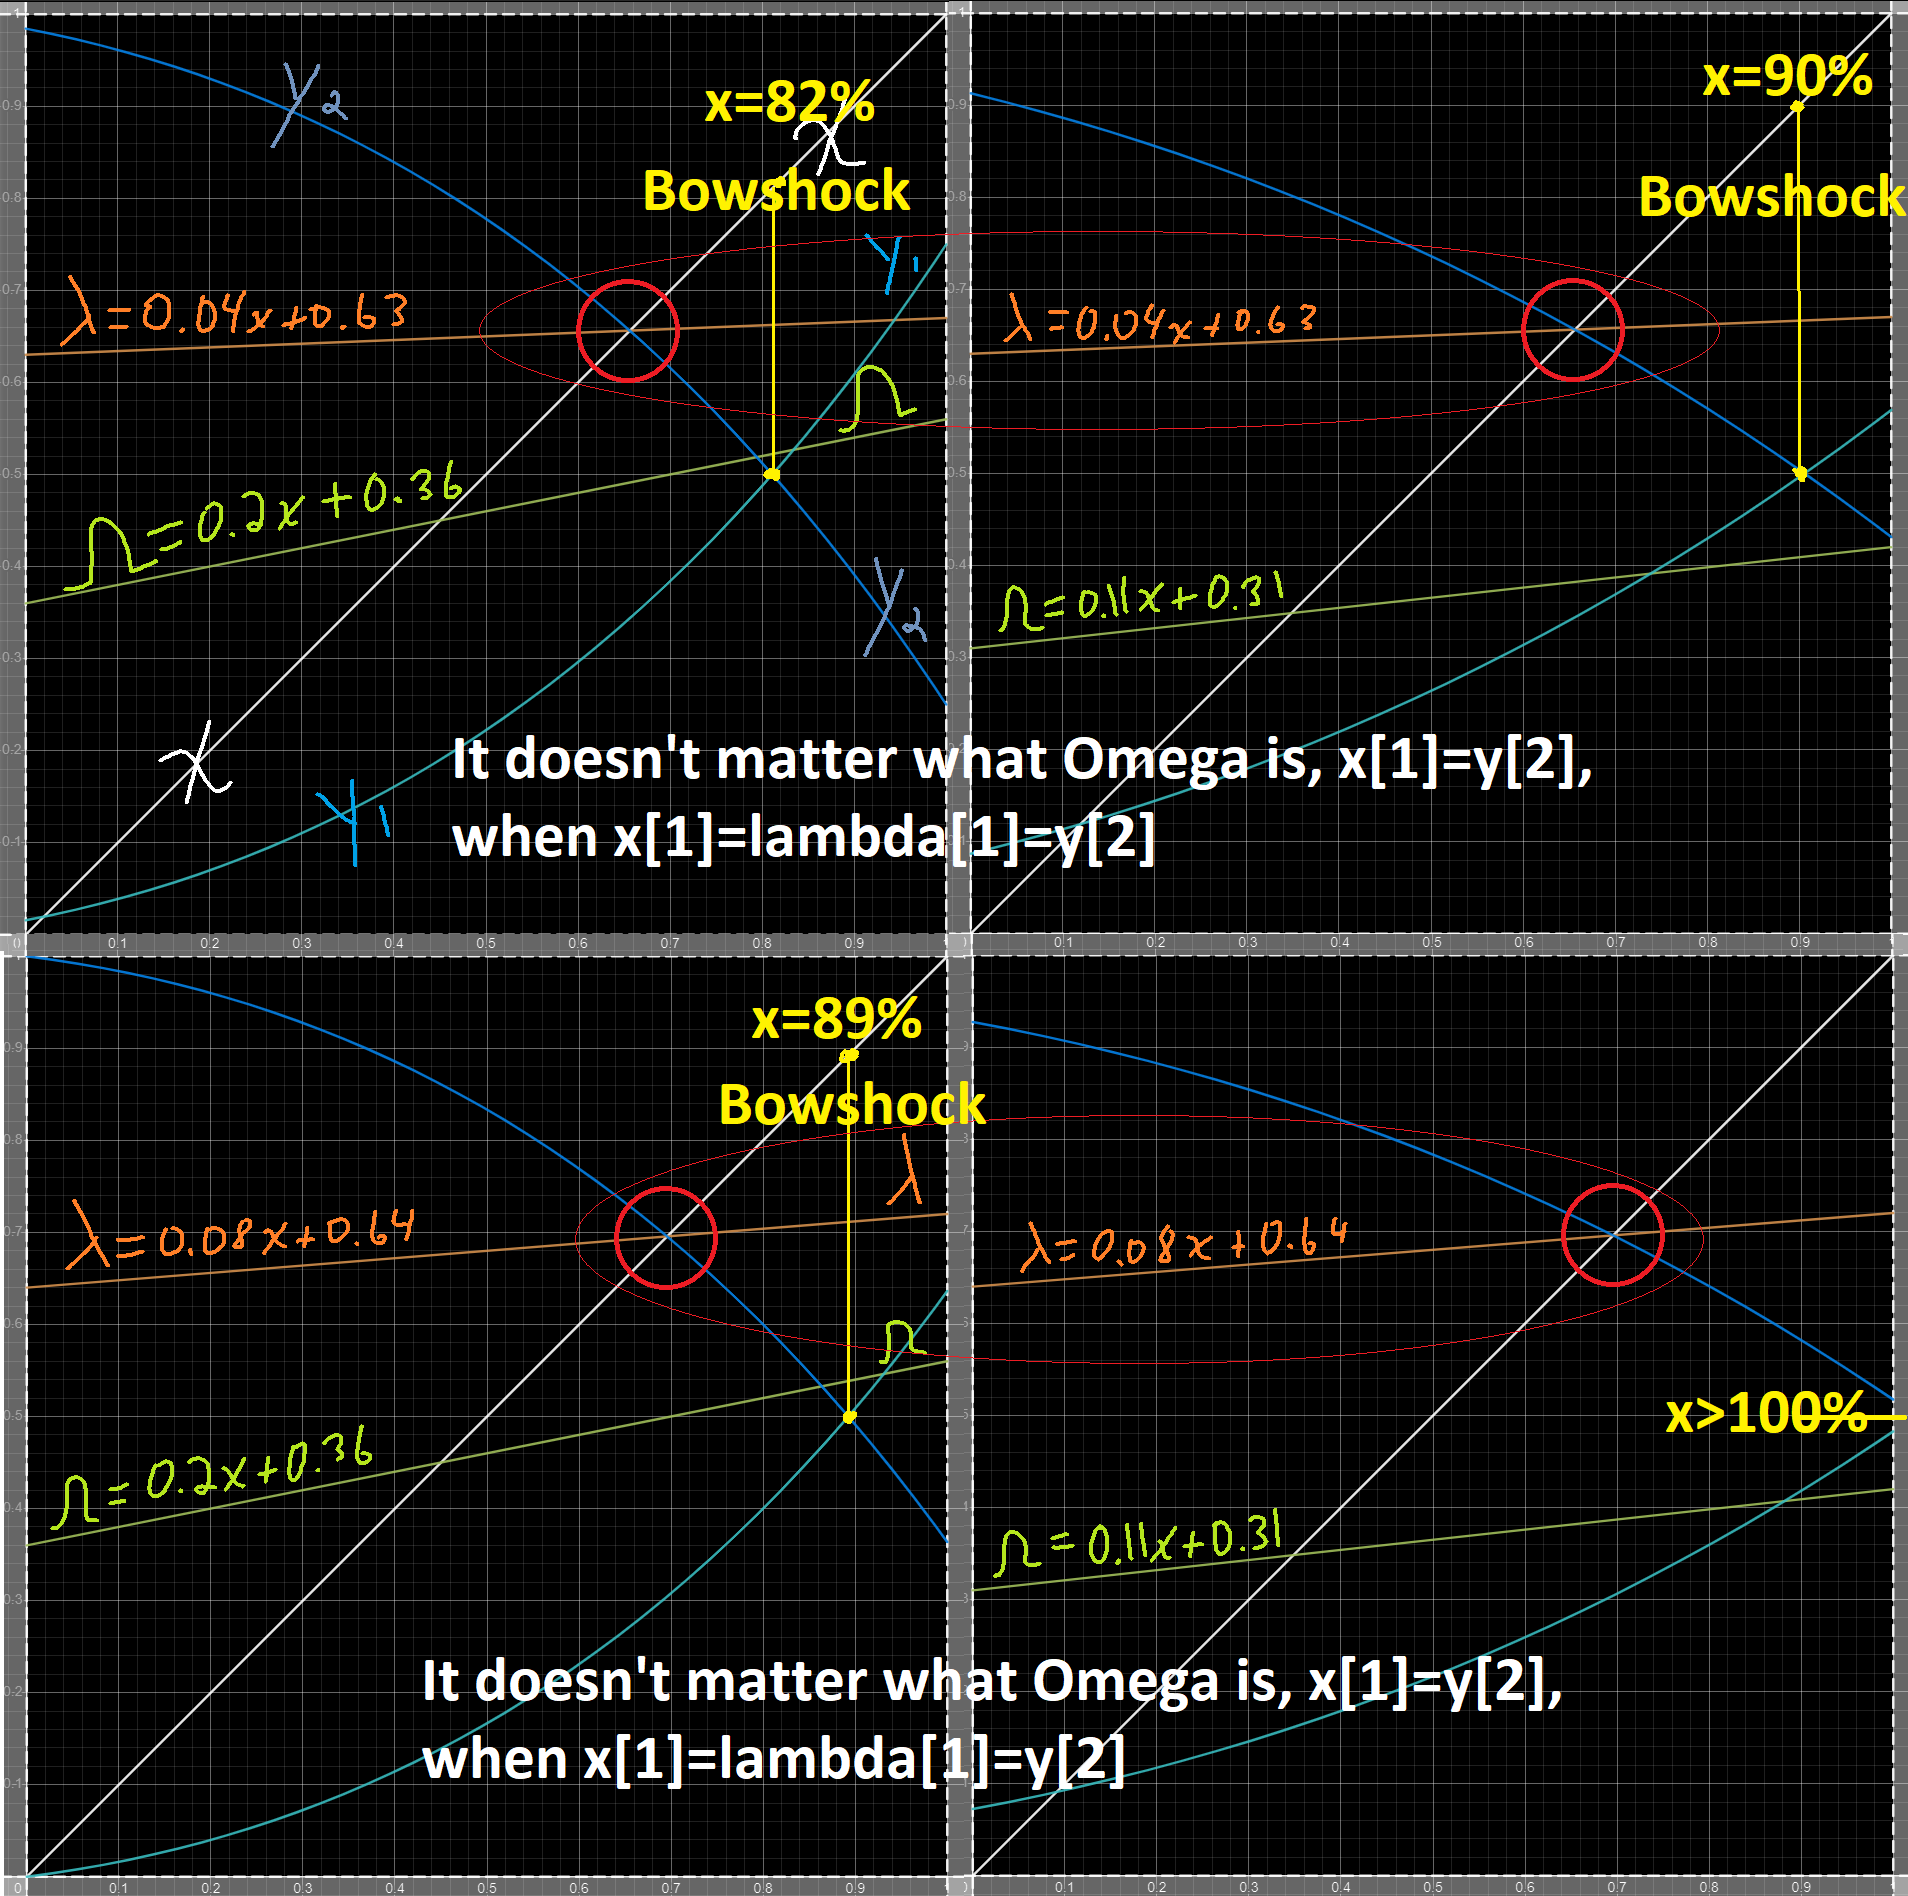
\includegraphics[width=275pt]{Sixth Law, x,lambda,omega.png}
\end{center}
\end{figure}
\newpage
For the Contrarians or Deceivers (it becomes difficult to tell the difference between contrarians and deceivers once I am this deep into the presentation), that oppose the diagram of the Sixth Law (which they technically can't oppose, because it's geometry), on the grounds that the Early Percentage (or election day percentage), $x_{1}$, may not be the proper horizontal axis to describe the election, we have the Fourth and Eighth Laws which use $\alpha$ as the horizontal axis.

The below graphs focus primarily on the Eighth Law, since the Fourth Law concerns the value of $x_{1}$ in respect to $\alpha_{1}, \lambda_{1}$ and $\Omega_{1}$. 

We know from the Twixt Lemma that $\alpha_{1}$ must exist between $x_{1}$ and $y_{1}$, and since the trajectory of $y_{1}$ is below $\alpha_{1}$ in the below graphs, we know that $x_{1}$ is above $\alpha_{1}$.

Under the Eighth Law, the Republicans cannot achieve more than 50\% of the Mail-in Vote, $y_{1}$, until $\alpha_{1}$ surpasses $\lambda_{1}$. More specifically $y_{1}=y_{2}$ when $\alpha_{1}=\lambda_{1}$. You can interact with these graphs here: \url{https://www.desmos.com/calculator/zl0aydge2b}
\begin{figure}[bp!]
\begin{center}
\caption{The Eighth Law: The Democrat Mail-in Percentage vs Alpha, Lambda and Omega.}
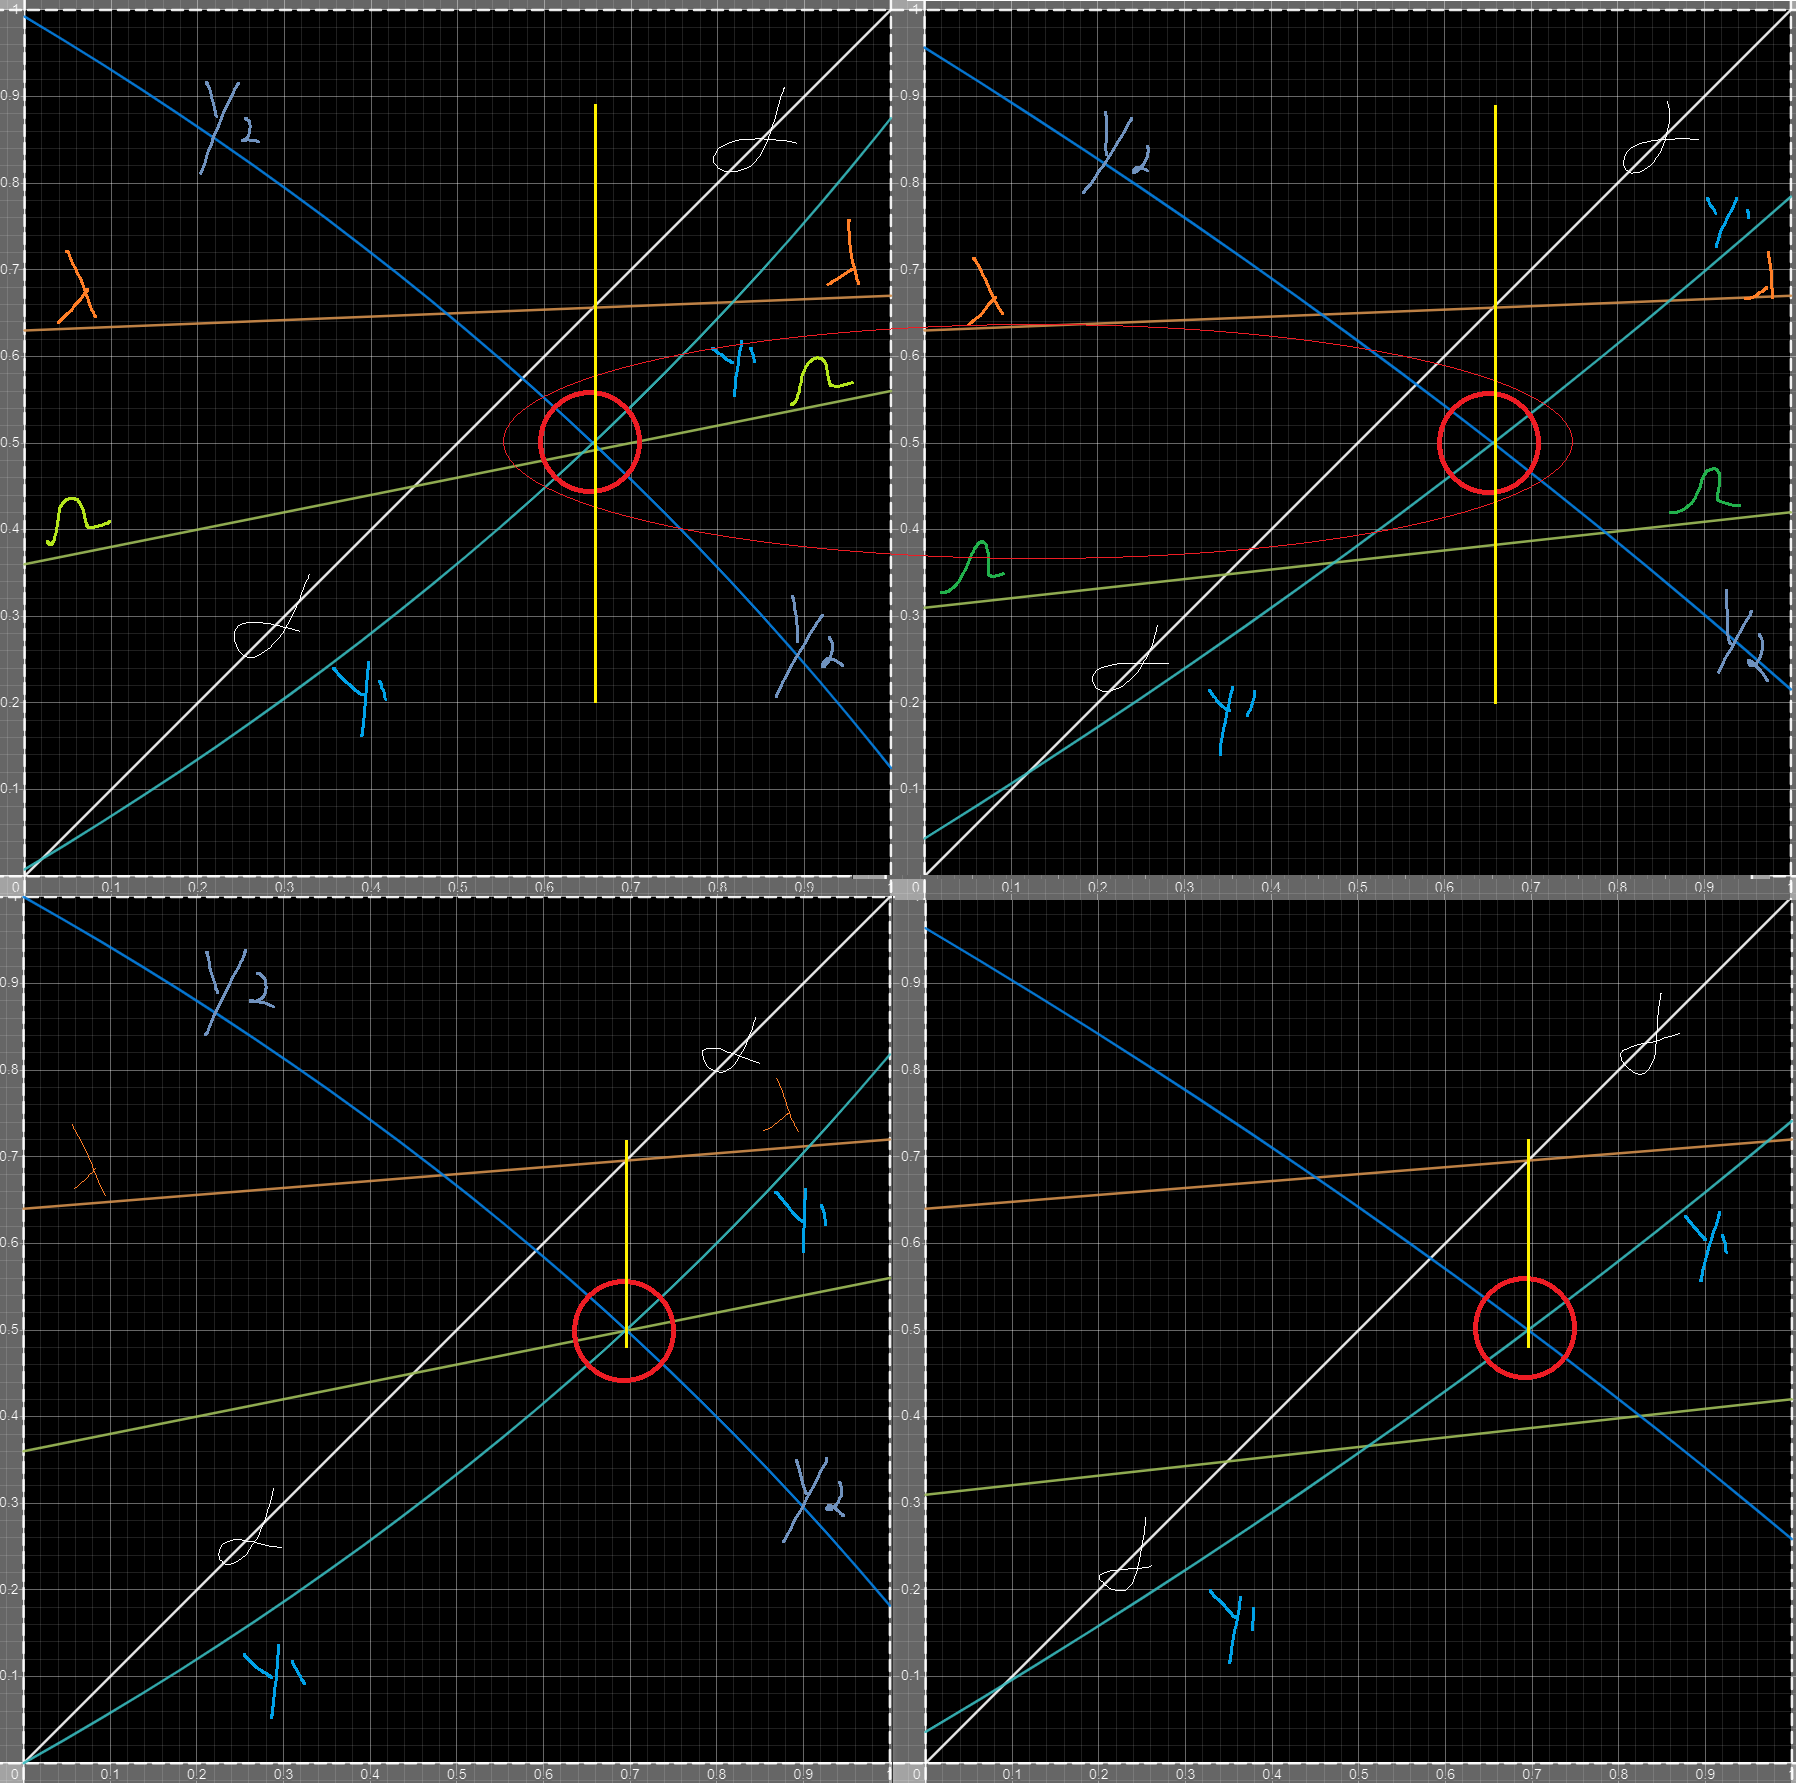
\includegraphics[width=275pt]{Fourth and Eigth Law.png}
\end{center}
\end{figure}
\newpage
\begin{theorem}{The Fifth Perversion Theorem, The Insurmountable Theorem--- The Insanity of Invariant Lambda}

That under the Eighth Law, that if $\lambda_{1}$ is generally invariant in respect to $\alpha_{1}$, and that the mean value of $\lambda_{1}$ is greater than 50\%, that the Republicans must achieve an aggregate percentage, $\alpha_{1}$, equal to the mean value of $\lambda_{1}$, until they are permitted to receive more than 50\% of the Mail-in Vote.

As it is in the case of Nevada, where the mean value of $\lambda_{1}$ is 63.5\%, with no meaningful variation, and even worse, with a positive incline in respect to $alpha_{1}$, it creates an \textbf{Insurmountable Burden} upon the Republican Electorate, that the better they perform in the Early Vote (or election day vote) the more difficult it becomes for them to acquire 50\% of the Mail-in Vote, such that they must acquire nearly 65\% of the total vote to achieve a Mail-in Percentage of 50\%.

Proof:
Let $s,t,u,v$ be the Republican Early Vote, Democrat Early Vote, Republican Mail-in Vote and the Democrat Mail-in Vote respectively, then:

$\lambda_{1}=\frac{s+v}{(s+v)+(u+t)}; \lambda_{2}=\frac{u+t}{(s+v)+(u+t)}$

$\alpha_{1}=\frac{s+u}{(s+u)+(t+v)}; \alpha_{2}=\frac{t+v}{(s+u)+(t+v)}$

$\Omega_{1}=\frac{s+t}{(s+t)+(u+v)}; \Omega_{2}=\frac{u+v}{(s+t)+(u+v)}$

$y_{1}=\frac{u}{u+v}; y_{2}=\frac{v}{u+v}$

Proof One:
$$\alpha_{1}=\lambda_{1} \iff u=v \iff y_{1}=y_{2}=50\%$$
Proof Two: The Eighth Law states...
$$y_{1}=\frac{\lambda_{2}+\alpha_{1}-\Omega_{1}}{2\Omega_{2}}; y_{2}=\frac{\lambda_{1}-\alpha_{1}+\Omega_{2}}{2\Omega_{2}}$$

$$y_{1}=y_{2} \implies \frac{\lambda_{2}+\alpha_{1}-\Omega_{1}}{2\Omega_{2}}=\frac{\lambda_{1}-\alpha_{1}+\Omega_{2}}{2\Omega_{2}}$$

$$\lambda_{2}+\alpha_{1}-\Omega_{1}=\lambda_{1}-\alpha_{1}+\Omega_{2} \implies \lambda_{1}-\lambda_{2}=2\alpha_{1}-1$$
$$\lambda_{1}-\lambda_{2}=2\alpha_{1}-1 \implies \lambda_{1}+(1-\lambda_{2})=2\alpha_{1}=2\lambda_{1} \implies \alpha_{1}=\lambda_{1} \iff y_{1}=y_{2}=50\%$$
\begin{flushright}
\textbf{Q.E.D}
\end{flushright}
\end{theorem}
\newpage
\begin{theorem}{The Sixth Perversion Theorem, The Obstacle Theorem---The Insanity of Invariant Lambda}

That under the Sixth Law, that if $\lambda_{1}$ is generally invariant in respect to $x_{1}$, and that the mean value of $\lambda_{1}$ is greater than 50\%, that Republicans must achieve an Early Day Percentage (or Election Day Percentage), $x_{1}$, that is equal to the mean value of $\lambda_{1}$, until Democrats will receive less than $\lambda_{1}$\%

As it is in the case of Nevada, where the mean value of $\lambda_{1}$ is 63.5\%, with no meaningful variation, and even worse, with a positive incline in respect to $x_{1}$, it creates a \textbf{ Geometrically Forced Obstacle} against the Republican Electorate, that the Democrat Mail-in Percentage cannot fall below 63.5\% until Republicans have achieved an Early Percentage of 63.5\%, in other words, Republicans are forced to acquire a 36.5\% Mail-in Percentage when they receive 63.5\% of the Early Vote---a 27 point difference.

This Theorem is derived directly from the Twixt Lemma, which states that $\lambda_{1}$ must exist between $x_{1}$ and $y_{2}$.

Proof:\\
$\lambda_{1}=\frac{s+v}{(s+v)+(u+t)}; x_{1}=\frac{s}{s+t}; y_{2}=\frac{v}{u+v}$

$$x_{1}=\lambda_{1}=y_{2} \implies \frac{s}{s+t}=\frac{s+v}{s+v+u+t}=\frac{v}{u+v}$$

$$\frac{s}{s+t}=\frac{s+v}{s+v+t+u} \implies s^2+sv+st+su=s^2+sv+st+tv \implies  su=tv$$

$$\frac{v}{v+u}=\frac{s+v}{s+v+u+t} \implies sv+v^2+uv+tv = sv+v^2+su+uv \implies su=tv$$

$$\frac{s}{s+t}=\frac{v}{u+v} \implies su+sv = sv+tv = sv+v^2+su+uv \implies su=tv$$
\begin{flushright}
Proof by the Reflexive Property.
\textbf{Q.E.D}
\end{flushright}
\end{theorem}
\newpage
\subsection{The Eight Problems of the 2020 Election of Trump vs Biden in Clark and Washoe Counties}
We shall temporarily dispense with the terms ``North, South, West, East and Diagonal vs Diagonal" for the remainder of this chapter.

So allow me to state, in Plain English, as I would to the General Public and the Citizens of a Jury, the Eight Main Problems in Clark and Washoe Counties in the 2020 Election of Trump vs Biden (these extend to the 2022 Primaries and the 2022 General Election of 2022, and there's even more problems in places like Atlanta (Georgia), Will County (Illinois), Macomb and Oakland Counties (Michigan), Maricopa (Arizona) and Philadelphia (Pennsylvania), where we find highly curved and deterministic manifolds of $g,h,\alpha)$

Let S be Trump's Early Vote at a precinct (a precinct is a voting station), let T be Biden's Early Vote at the same precinct, let U be Trump's Mail-in vote at the same precinct, let V be Biden's Mail-in Vote at the same precinct. Let K be the sum of all ballots cast at the precinct, K=S+T+U+V.

Let $x,y,c,\alpha$ be the Election Percentages, since they describe Trump's Early Percentage, Trump's Mail-in Percentage, Biden's Mail-in Percentage and Trump's Total Percentage in each precinct, where:

$x=\frac{S}{S+T}; y=\frac{U}{U+V}; c=\frac{V}{U+V}; \alpha=\frac{S+U}{K}$

Let $m,n,d,\Omega$ be the Preference Percentages, since they describe the percentage of Trump Voters to cast their ballot early, percentage of Biden Voters to cast their ballot early, percentage of Biden Voters to cast their ballot by mail, and the percentage of all Voters who prefer to cast their ballot early, respectively.

$m=\frac{S}{S+U}; n=\frac{T}{T+V}; c=\frac{V}{T+V}; \Omega=\frac{S+T}{K}$

Let $g,h,\lambda$ be the Strange Percentages, since they are the remaining three percentages which have no verbal description, as they do not represent a particular preference or behavior of the electorate. These percentages exist only as mathematical abstractions, and should have no significance in a fair election.

Let $g=\frac{S}{S+V}$ be the percentage of ballots cast that are Trump Early ballots amongst Trump Early and Biden Mail-in Ballots at the precinct.\\
Let $h=\frac{U}{U+T}$  be the percentage of ballots cast that are Trump Mail-in ballots amongst Trump Mail-in and Biden Early Ballots at the precinct.\\
Let $\lambda=\frac{S+V}{K}$ be the Percentage of all Ballots Cast that are either Trump Early Ballots or Biden Mail-in Ballots at the precinct.
\newpage
In accordance to the above definitions of $S,T,U,V,x,y,g,h,m,n,\alpha,\Omega,\lambda,c$ and $d$, the following eight problems arise in Clark and Washoe Counties, in the 2022 General Election of Trump vs Biden, which, beyond all reasonable doubt, conclude that the election was manipulated. Each of these problems arise from the fact that $\lambda$ is generally invariant over the precincts, with a mean value of 63.5\% with a small standard deviation of 3\%.

First Problem: That since $\lambda$ is invariant, it means we can calculate K knowing only S and V, that is K=(1/0.635)(S+V), which means the total ballots cast was determined by Trump's Early Vote and Biden's Mail-in Vote, which is impossible because Trump's Mail-in Vote and Biden's Early Vote have yet to be counted. This places a restriction on Trump's Mail-in Vote, that it can never exceed 36.5\% of all ballots cast, while Biden's Mail-in Vote can go to 63.5\% of all ballots cast. This is tremendous barrier for Trump, since he must perform incredibly in the Early Vote to win the election.

Second Problem: That since $\lambda$ is invariant, it means we can calculate Biden's Mail-in Vote, V, knowing only K and S, that is V=63.5\%K-S, and this formula has an $R^2>0.98$ across the 1286 precincts. This is impossible because it means that the total ballots cast, K, determined Biden's Mail-in Vote, V, before Biden's Mail-in Vote was known, yet K, the Total Ballots Cast, cannot have been known until after all ballots were cast, including Biden's Mail-in ballots, V, in each precinct.

Third Problem:  The invariance of $\lambda$ itself is a concern, because it does not represent a preference or behavior of the voters. Imagine that $\alpha$ was invariant over the precincts, this would be very strange, as it would state that in every precinct, Trump got the same percentage of the vote...but at least we can put this strange scenario in words. Likewise if $\Omega$ was invariant over the precincts, it would also be strange, as it would state that in every precinct, the preference to vote Early was same, yet again we can at least put this strange scenario in words. However, there is no way to comprehend the meaning of $\lambda$ being invariant over the precincts, because $\lambda$ does not even represent a preference or behavior of the voters. This makes the invariance of $\lambda$ very suspicious. How could the voters of Nevada make such a uniform decision across all 1286 precincts in Clark and Washoe Counties, two demographically different and distant counties on opposite sides of the State of Nevada? Even more distressing is that this a uniform decision that does not even represent a particular preference or behavior of the voters! Lambda is supposed to be a pure mathematical abstraction, not an actual entity that describes the election!

Fourth Problem: That $\alpha=g\lambda+(1-\lambda)h$. However, since $\lambda$ is invariant over the precincts, we have $\alpha=g(0.635)+(0.365)h$ for every precinct. This formula has an $R^2$ exceeding 0.995 over all 1286 precincts.  This means that the $(g,h,z)$ coordinates collapse to a flat plane, instead of a 3D Gaussian cloud of probability, since in a fair election, $g$ and $h$ alone cannot determine $\alpha$, without knowledge of $\lambda$, yet in this election we can solve for $\alpha$ with from only $g$ and $h$ with no knowledge of any precinct's $\lambda$.

Fifth Problem: That $\alpha=g\lambda+(1-\lambda)h$   However, since $\lambda$ is invariant over the precincts, we have $\alpha=g(0.635)+(0.365)h$ for every precinct. This formula has an $R^2$ exceeding 0.995 over all 1286 precincts.  This means that the $g$ and $h$ percentages, which don't even represent a preference or behavior of the voters, have formed a deterministic manifold that yields Trump's Aggregate Percentage in each precinct, that allows us to solve for $\alpha$ without knowledge of $\lambda$. It is \textbf{incredibly damning} that the Election of 2020  can be described deterministically in terms of $g$ and $h$, when neither $g$ nor $h$ describe a particular behavior or preference of the voters.

Sixth Problem: That $c$, which is Biden's Mail-in percentage, can be expressed as $c=\lambda+(\frac{\Omega}{1-\Omega})(\lambda-x)$, which is the geometric relationship between $c,w,x$ and $\Omega$. It states that $c$ is the reflection of $x$ over the value of $w$, scaled by $\frac{\Omega}{1-\Omega}$. Thus when $x=\lambda$, then $c=\lambda$, therefore $x=c$ if and only if $x=\lambda$. Thus, since $\lambda$ is invariant over the precincts with a mean value of 63.5\%, this geometric relationship says that Biden cannot get less than 63.5\% of the mail-in vote in any precinct until Trump gets more than 63.5\% of the Early Vote, and when Trump does achieve this, that he will still only have 36.5\% of the mail-in vote, geometrically forcing a 27\% difference between Trump's Early and Mail-in Percentages.  More generally, the invariance of $\lambda$ (and the fact that $\lambda$ is on a slight positive incline in respect to $x$) at 63.5\% causes the difference between $x$ and $y$ (Trump's Early and Mail-in Percentages) to grow continuously, meaning the better Trump performs in the Early Vote, the more Trump suffers in the Mail-in Vote, regardless of the value of $\Omega$, which is the percentage of all voters that cast their ballots early.

Seventh Problem: That $c$, which is Biden's Mail-in Percentage, can be expressed as $c=\frac{\lambda-\alpha+(1-\Omega)}{2(1-\Omega)}$, and that $y$, which is Trump's Mail-in Percentage, can be expressed as $c=\frac{(1-\lambda)+\alpha-\Omega}{2(1-\Omega)}$, which states that $c=y=50\%$, if, and only if, $\alpha=\lambda$.  However, since $\lambda$ is invariant over the precincts at 63.5\%, it means that Trump must acquire at least 63.5\% of the total vote, before his mail-in percentage can exceed 50\%. This places an nearly insurmountable obstacle in Trump's way, since he must perform extremely well (well beyond 63.5\%) in the Early Vote to achieve an aggregate percentage of 63.5\%.

Eighth Problem:That $n$, which is percentage of Democrats that prefer to vote Early, can be expressed as $n=\frac{(1-\lambda)(1-x)m}{\lambda x+m(1-2x)}$. In the 2020 election, the trajectories of $m$ and $w$ were parallel in respect to $x$ (with a mean difference less than 3\% between their trajectories), and since $w$ has a mean value of 63.5\% with no meaningful variation, it forces $n$ to decreases rapidly with $x$, meaning the Democrat mail-in turnout increases rapidly as Republicans perform better in the early vote.

From these Eight Problems, we can conclude, beyond a reasonable doubt, the 2020 General Election of Trump vs Biden in Clark and Washoe Counties, Nevada, was rigged.

We can also conclude, beyond all reasonable doubt the either one of the following two mechanisms were used to achieve this uniformity of $\lambda$ over the precincts (which caused all of this erratic behavior), and follow from the fact the linear regression of K (the total number of Early and Mail-in Ballots cast at a precinct) in terms of S and V (Trump's Early Vote and Biden's Mail-in Vote) was $K=1.4243S+1.6862V$, with an $R^2=0.988$ with a coefficient of multiple correlation of 0.994.

Mechanism One (least likely): That the Total Ballots Cast was determined by Trump's Early Vote and Biden's Mail-in Vote, and then a great portion of Trump's Mail-in Vote was deleted to achieve the new Total Ballots Cast.

Mechanism Two (more likely), that when the total ballots cast was known, that Biden's Mail-in Vote, V, was reset via the formula $V=\frac{K-1.42433S}{1.6862}=0.5930K-0.8446S$, and that the requisite number of Trump Mail-in ballots were intentionally miscounted as Biden Mail-in Ballots until the new number for V was achieved. The constants of the formula were chosen to achieve a statewide victory for Biden, using the two most populated counties, Clark and Washoe, on opposite sides of the State Nevada, to counteract the result in the other counties and to counteract the overwhelming legitimate popularity of Trump in Clark and Washoe Counties.

It should also be noted that this formula: $V=0.5930K-0.8446S$ will in fact produce a small artificial variation in $\lambda$ and create the slightly inclined of the trajectory of $\lambda$ in respect to $x$ and $\alpha$, and also cause $m$ to be nearly parallel the trajectory of $\lambda$ with a small difference around 3\% between their trajectories, which was observed in the actual election, and also leads to a massive divergence between the Early and Mail-in Percentages as $x$ and $\alpha$ increase and massive increase in Democrat Mail-in Turnout, $n_{2}$, as $x$ and $\alpha$ increase, and also creates the observed Cubic Torsion in the Manifold of $g,h,\alpha$ (that is, the manifold of $g,h,\alpha$ is not perfectly flat, but rather curved, although nearly imperceptible to the human eye).
\newpage
Mechanism Three (most probable): That, when taking into consideration the curved manifolds of $g,h,\alpha$ in other States, such as Illinois, Pennsylvania, Georgia, Michigan and Arizona, and the fact that the manifold of $g,h,\alpha$ in Nevada also has slight curvature (which produces a small artificial variation in $\lambda$, and the fact that these manifolds are quaternionic in Illinois and Nevada in 2022 (a quaternionic manifold that rigs four countywide/statewide races at a time), that a Hypercomplex Valued Neural Network, also known as an HVNN (or an ELM for Extreme Learning Machine), manipulated the individual values of $g$ and $h$ in each precinct, and set $alpha$ accordingly to a manifold formula, to minimize the following Cost Function across the precincts:

Cost One: To minimize the difference between the Republican Aggregate Performance in the previous election cycle to the manifold value of $alpha$ in the current election, in each precinct.

Cost Two: A Countywide Cost on the angular value of the principal $m,n$ eigenvector, in order to perpetuate the myth the Democrats prefer to vote by mail, while not caring about the 3D principal eigenvector of $m,n,\alpha$.

Cost Three: The minimize the number of ballots created, destroyed, or flipped at each precinct by distributing the entire load of the fraudulent ballots over the precincts in respect to the number of registered voters (which is the algorithmic size of the precinct).

Cost Four: At each precinct, the minimize the difference between the $\Omega$ values across the races of that precinct (to ensure the same proportion of Early to Mail-in Votes across the races at the same precinct), which is why the Quaternions are used.

Cost Five: To minimize the difference in the aggregate percentages between candidates of the same party, while slightly favoring one candidate of the same party over another candidate in different races, using the the quaternions to distribute the magnitude of the $\alpha$ vector disproportionately amongst candidates of the same party in different races (which is why the Republican, Lombardo, won the Gubernatorial Race, while the other Republicans lost down the ballot in 2022).
\newpage
Cost Six: To minimize the above costs while ensuring the the selected slate of candidates win their respective elections (infinite cost if not fulfilled, which would be programmed using a massive hyperbolic cost function that is effectively zero when the result of the election is below the Automatic Recount criteria of the State, and balloons to infinity the moment any particular selected candidate loses).

We shall cover the quaternionic manifolds of Illinois 2022 and Nevada 2022 in the final chapter. Given all of the above, the Third Mechanism is the most likely, since it explains the rig in the other States using the same system in Nevada. 

It is only because the manifold of Nevada was nearly flat (almost imperceptible curvature) that the irregularities are easy to explain to general public. I'm personally convinced it was an Act of G-d that the cubic manifold constants of Nevada resulted in a nearly flat plane. By Nevada's $g,h,\alpha$ being nearly flat, it caused $\lambda$ to be nearly constant at 63.5\% across the precincts. 

In other words, the constancy of $\lambda$ was an unintended consequence of rigging the election with a manifold that was nearly flat (thus, peculiar to Nevada). In other rigged elections, that exhibit eccentrically curved $g,h,\alpha$ manifolds, we do not get a constant lambda, and thus the results of election cannot be reduced in simpler terms to the general public, which is Nevada is a G-dsend.
\newpage
\subsection{What is the Trajectory of Lambda in Fair Election? No Basis for Democrats Preferring To Vote by Mail}
A common question asked of me at this point in the presentation (or article) is the expected trajectory of lambda in respect to $x,y$ and $\alpha$ in a fair election. 

Although it's fine for the ordinary layman to ask this question, I sigh when this asked by credentialed mathematician, because the Twixt Lemma, the Single Aggregate Convergence Lemma and the Irrelevance Theorem already provides a concise answer to this question.

The trajectory of Lambda is bounded between the Republican Election Day (or Early) Percentage, $x_{1}$, and the Democrat Mail-in Percentage, $y_{2}$. The mean value of $\Omega$ determine the trajectory of $\lambda$ between $x_{1}$ and $y_{2}$, and the standard deviation of $\lambda$ is tied directly to the standard deviation of $\Omega$.  

If the mean value of $\Omega$ is 50\%, then the mean value of $\lambda$ is also 50\% with a flat trajectory, since it means that $\lambda$ must bisect the lines $x_{1}=x_{1}$ and $y_{2}=1-x_{1}$. As the mean value of $\Omega$ approaches 0\%, $\lambda$ follows $y_{2}$, and as the mean value of $\Omega$ approaches 0\%, $\lambda$ follows $x_{1}$.

Before I present the graphs and tables for the expected means and standard deviations of $\lambda$, these tables are made under the assumption that there is no difference in the preference between Democrats and Republicans to cast their ballots Early or by Mail, just as there is no difference between Democrats and Republicans to prefer vanilla or chocolate ice-cream.

\textbf{Until someone can show me a fair election where Democrats prefer to vote by Mail---that is an election that has no manifolds that violate any of the Twenty Laws and Forty Isometries, nor fails a Quantile Secant Test (Chapter Three)---and makes available the tabulations by Counting Group (Election Day, Early and Mail-in) for each precinct from the \textcolor{red}{certified totals} of County Recorder/Secretary of State/Registrar of Voters, you have \textcolor{red}{NO RIGHT TO CLAIM} that ``Democrats Prefer to Vote by Mail."}

PROVE IT. Find me an election where Democrats Prefer to Vote by Mail that doesn't have a manifold. I dare you.

We do science here. We do geometry. We do the Twenty Laws and Forty Isometries. If you want to show that Democrats prefer to vote by mail---prove it. So far all have failed, and some have been reduced to tears after having done their own research looking for a fair election where $n<m$ and finding only deterministic manifolds of $g,h,\alpha$ nationwide.

Until then, we shall assume that $x_{1}=y_{1}$ and $m_{1}=n_{1}$ in a fair election (more specifically, the eigenvectors are at 45 degrees with no significant offset).
\newpage
In the below diagram, you see the values of $x_{1}, y_{1},\alpha_{1}$ and $\lambda_{1}$ (pink, blue, purple and yellow respectively) graphed against the quantiles of $\alpha$. In the top three graphs, the mean value of $\Omega$ is set to 10\% with a standard deviation of 0.024\%; in the center graphs, the mean value of $\Omega$ is set to 50\% with a standard deviation of 12\%, and in the bottom three graphs the mean value of $\Omega$ is set to 90\% with a standard deviation of 0.024\%. 

The Left graphs are Republican Landslides, where mean $\alpha$ is 70\%, the Center Column of graphs are Neutral Election, where mean $\alpha$ is 50\%, and the Right Graphs are Democrat Landslides where the mean value of $\alpha$ is 30\%.

Notice that $x_{1}$ (pink) residuals are wide (Irrelevance Theorem) and the $y_{1}$ (blue) residuals are non-existent in the top graphs, this is because the mean value of $\Omega$ is 10\%, thus $\alpha$ and $y$ converge on each other, and $\lambda$ and $y_{2}$ converge upon each other.

In the bottom graphs, where the mean value of $\Omega$ is 90\% it's the other way around, both $\alpha$ and $\lambda$ converge on $x_{1}$. In the center graphs, where the mean value of $\Omega$ is 50\%, both the pink and blue residuals bespangle the trajectory of $\alpha$ and $\lambda$ has a slight negative tilt, regardless of the mean value of $\alpha$.
\begin{figure}[bp!]
\begin{center}
\caption{The Expected Trajectories of Lambda in a fair election.}
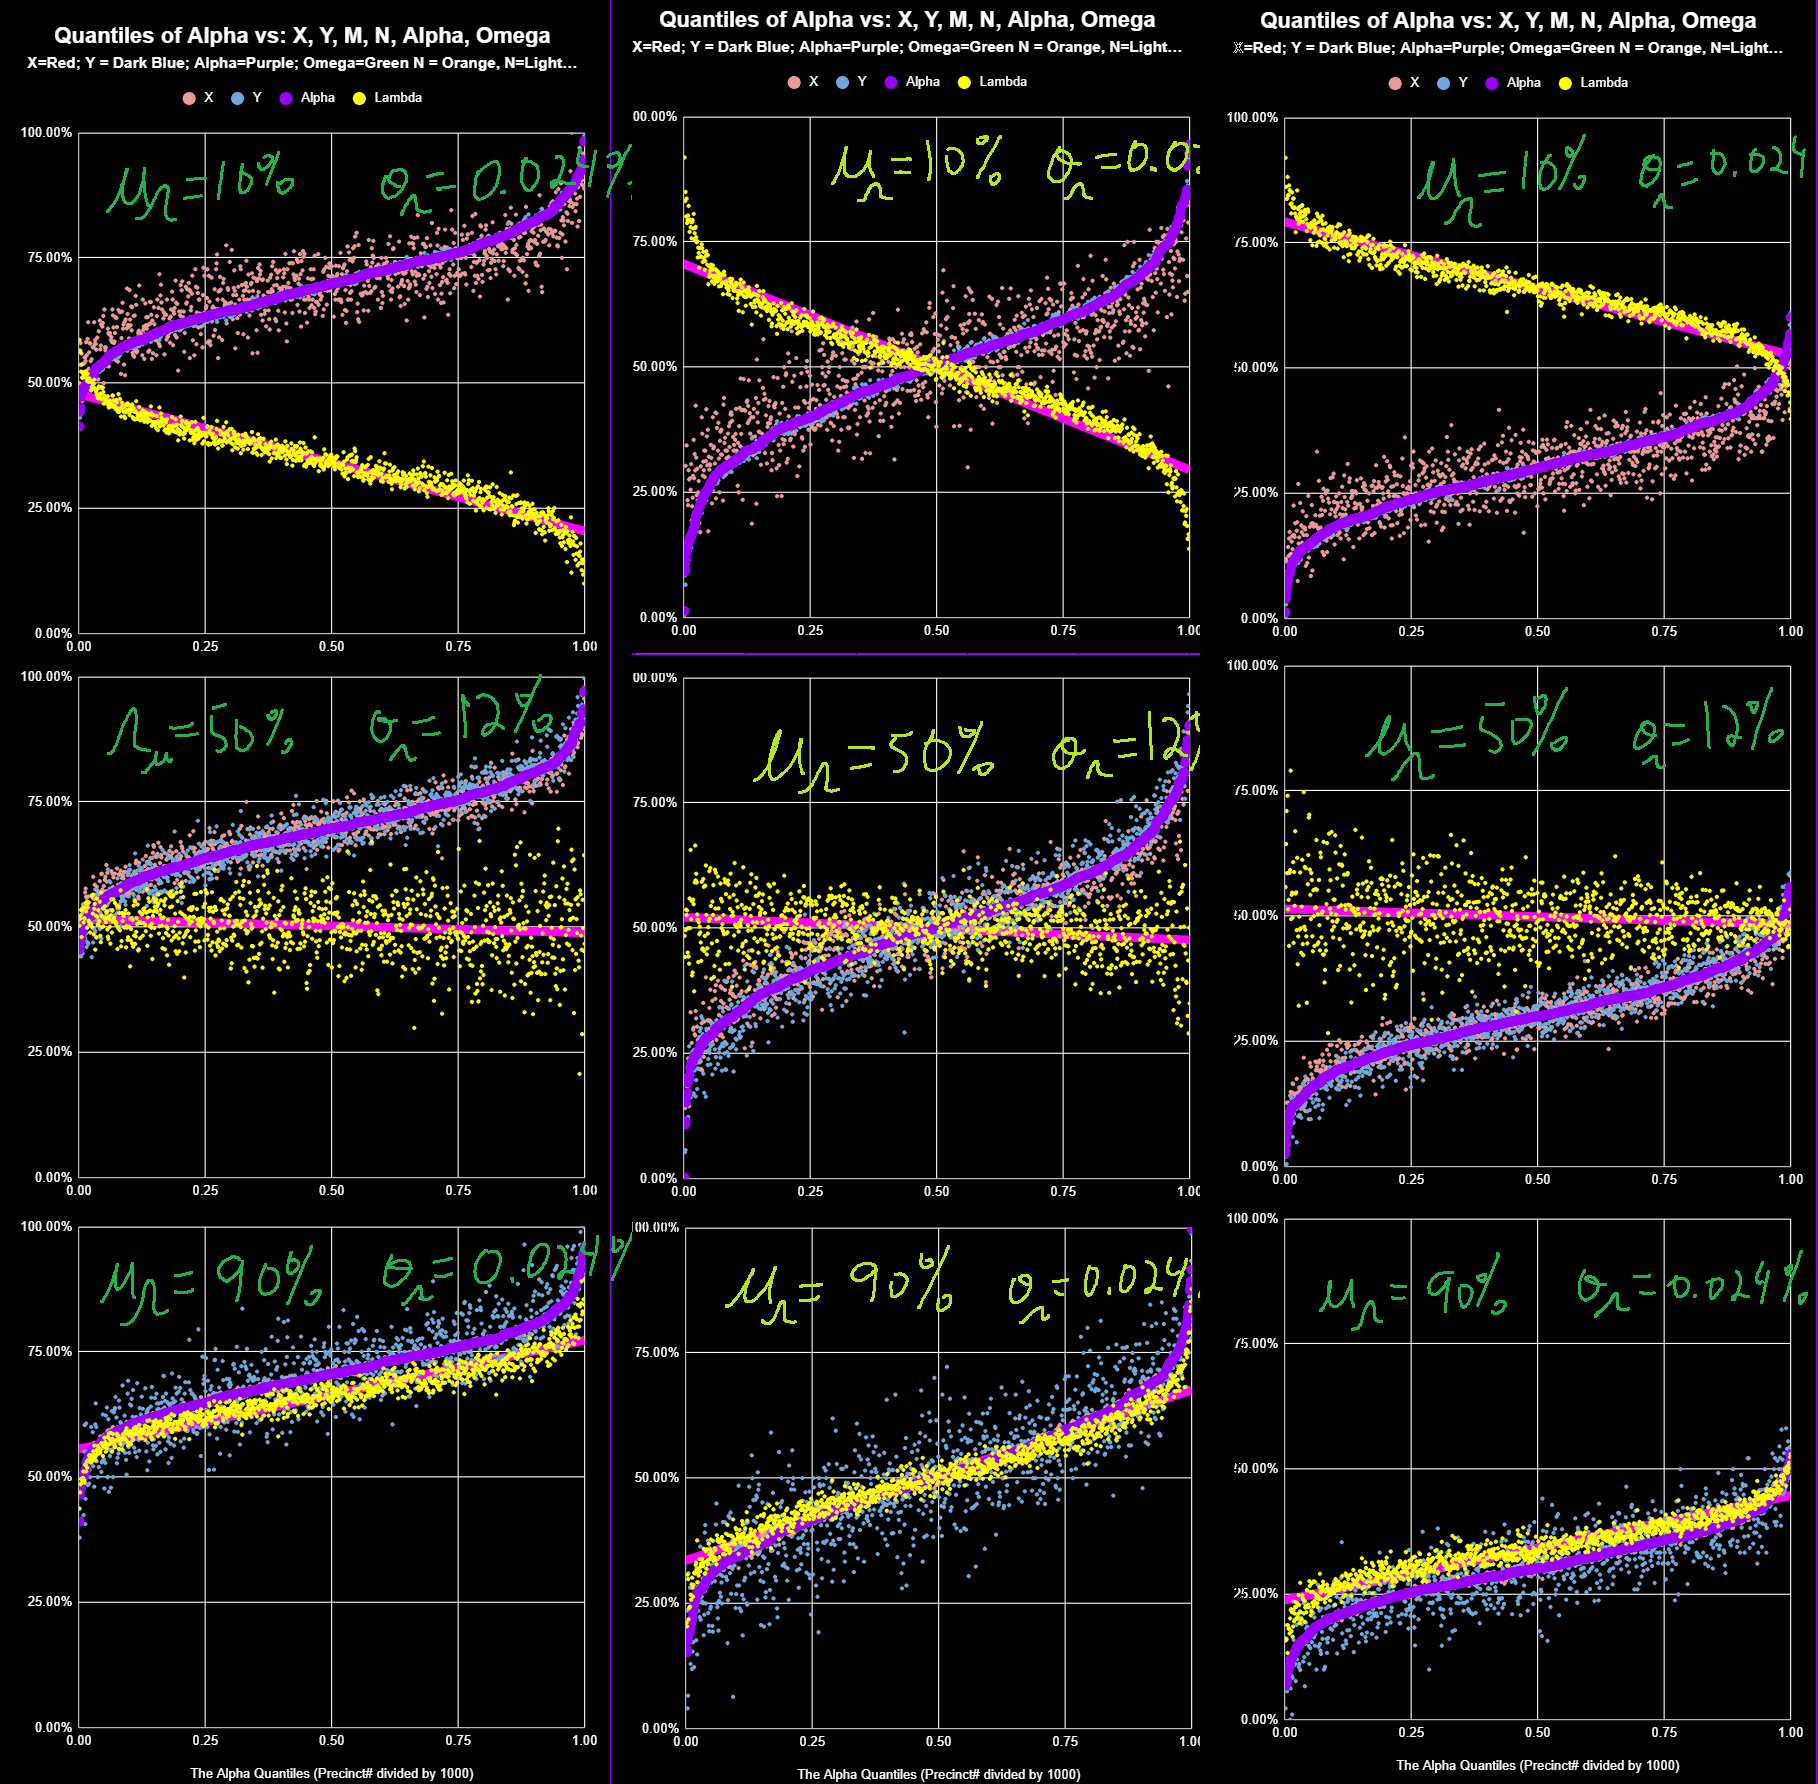
\includegraphics[width=275pt]{Fair Lambda.png}
\end{center}
\end{figure}
\newpage
In the below tables there two sets of Five Columns, titled ``Democrat Landslide, Democrat Win, Neutral, Republican Win, Republican Landslide," where the mean values of $x_{1}$ are 30\%, 40\%, 50\%, 60\% and 70\% respectively, with standard deviations of 8\%, 10\%, 13\%, 10\% and 8\% respectively, with a $y_{1}$ noise offsets of 5\%, 6.5\%, 8\%, 6.5\% and 5\% respectively. You interact and experiment with these parameters here: \url{https://docs.google.com/spreadsheets/d/1W7amfyeFUH62hF6biIg_IUrWyMUmcHawbpaoB3K9zNw/edit?usp=sharing}

The first set of five columns displays the expected mean value of $\lambda$ for row (where each row increments the mean value of $\Omega$ by 5\% and sets the standard deviation of $\Omega$ to $0.24\Omega$ when $\Omega \le 50\%$, and to $0.24(1-\Omega)$ when $\Omega > 50\%$). The second set of five columns show the expected standard deviation of $\lambda$ under the same conditions. Notice that the only time that $\lambda$ has a flat trajectory is when it has a mean value of 50\% (and when the mean value of $\Omega$ is also 50\%). This is what we expect in a fair election, because for $\lambda$ to have a flat trajectory anywhere else (like at 63.5\% in Nevada), means that one of the political parties (Republicans in Nevada) face an \textcolor{red}{Insurmountable Obstacle to Victory}.
\begin{figure}[bp!]
\begin{center}
\caption{The Expected Lambda Parameters in a Fair Election}
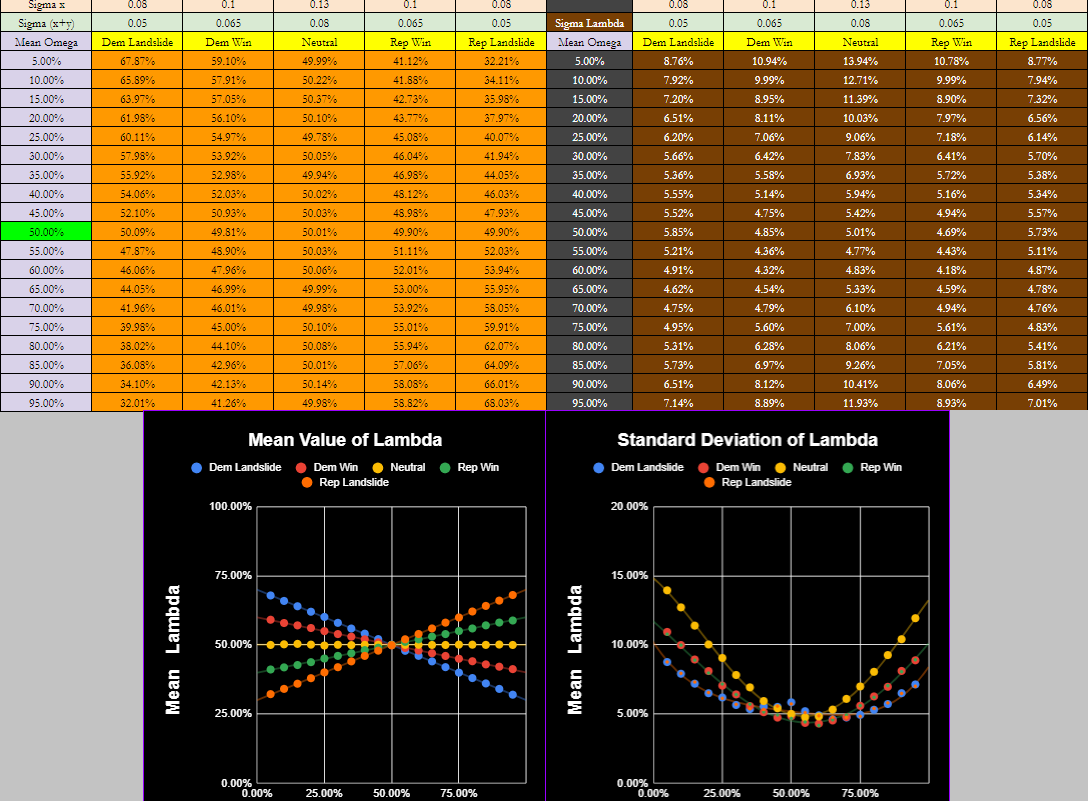
\includegraphics[width=400pt]{FairLambdaStats.png}
\end{center}
\end{figure}
\newpage
\subsection{2004 General Election of Bush vs Kerry, 2004, Fair Election, Clark and Washoe, X=Y and M=N !!!}

It seems in 2004, that \textcolor{red}{The Wisdom of Little Johnny the Fifth Grader prevailed} in both Clark and Washoe Counties.  

It's truly amazing how the eigenvectors of $(x+iy)$ and $(m+in)$ are both at 45 degrees in 2004! Isn't it amazing that Common Sense prevails in a fair election? 

Here is the spreadsheet of the County Recorder Tabulations for 2004: \url{https://docs.google.com/spreadsheets/d/1N-akflHx3iSmS_xGlAtqsXGkS-BKXxV4ZGVWP2egWvI/edit?usp=sharing}
\begin{figure}[bp!]
\begin{center}
\caption{Y=X and M=N (Parallel), 2004 Clark County}
\noindent\makebox[\textwidth]{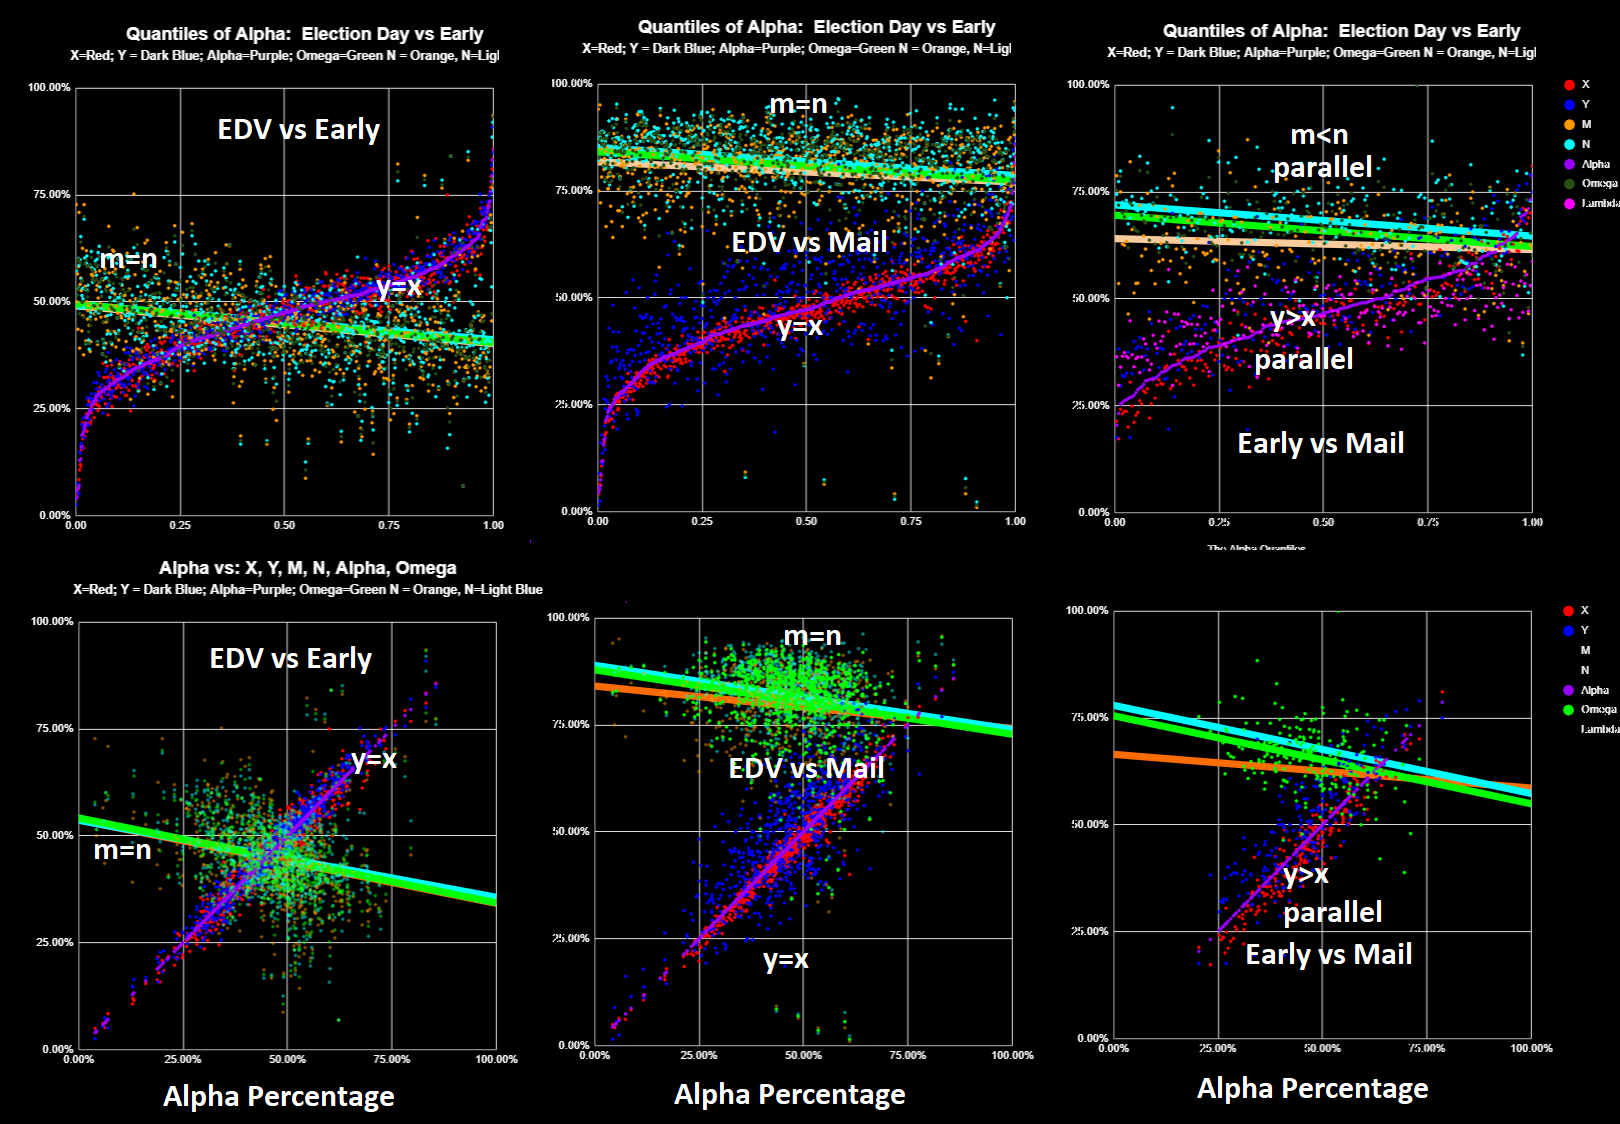
\includegraphics[width=500pt]{Clark 2004.png}}
\end{center}
\end{figure}

\newpage
In Washoe County, 2004, Little Johnny the Fifth Grader needs a little help from the PhD's and graduate students, Bard and ChatGPT AI's. There is a \textbf{small} constant difference between the $m$ and $n$ percentages; however, notice that they remain mostly parallel, meaning that non-political demographic factors affected both the Republican and Democrat Preference percentages at an equal rate. Notice that the bowshock of the Election Day vs Early Vote is at a tame value between 8\% and 12\%, as interviewed undergrads, grads and PhD's predicted in their drawings (and the Chatbot AI's!). For the Election Day vs Mail-in Vote, we get m=n and x=y, and for the Early vs the Mail-in vote we get parallel trajectories of m=n on a significant decline, and thus, as a result, y=x. 

In both Clark and Washoe, $\lambda$ behaves as predicted in the Fair Lambda Tables/Graphs in the previous section, such that $\lambda$ does not act as an Obstacle against either party. We'll discuss Clark's 2004 $\lambda$ on the next page.
\begin{figure}[bp!]
\begin{center}
\caption{$Y<X$; $N<M$; Parallel, Washoe 2004}
\noindent\makebox[\textwidth]{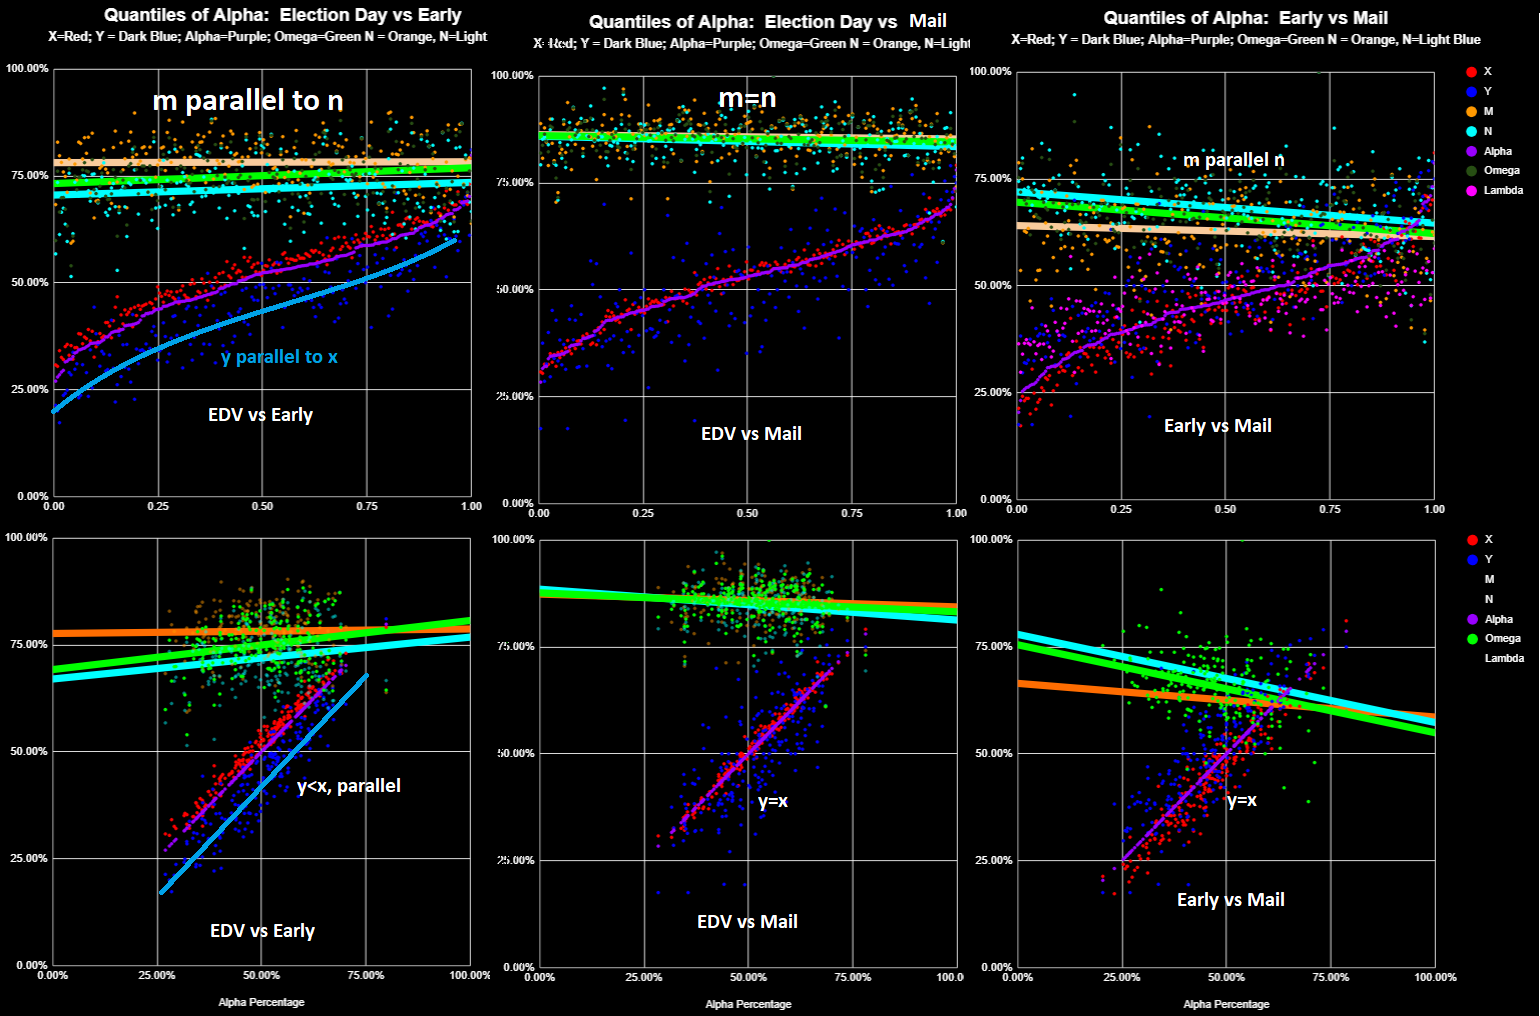
\includegraphics[width=500pt]{Washoe 2004.png}}
\end{center}
\end{figure}
\newpage
The below graphs show the $g,h,\alpha$ coordinates for Clark (blue) and Washoe (red) Counties in 2004. In Washoe, $g,h,\alpha$ form an ascending quadratic spiral for the Election Day vs the Early Vote, as expected (instead of the descending cubic domes of Atlanta Georgia and Will County Illinois).

And here is the part that is going to surprise you, in Clark County the $g,h,\alpha$ coordinates form a flat plane for the Election Day vs the Early Vote---\textbf{as expected,} with a mean value of $\lambda$ equal to 49.52\% with a standard deviation of 03.77\%. \url{https://plotly.com/~EKSolomon/106/}

The Fair Lambda Table/Graphs clearly show us that $\lambda$ will have a mean value of 50\% and a small standard deviation around 5\% and a flat trajectory over the quantiles of $\alpha$. Using the specific parameters of Clark 2004, such as mean value of $\Omega$ being at 45\% with a standard deviation of 09.5\%, and the mean noise of $y$ being -00.6\% with a standard deviation of 05.46\% and the mean value of $x$ being 46\% with a standard deviation of 12\%, we get an expected mean value of $\lambda$ at 50.59\% with a standard deviation of 03.87\%, which is pretty much equal to the actual election results at 49.52\% and 03.77\%.

Also bear in mind that $\lambda$ being at 50\% means that is not an Obstacle to either party. All it means is that you need 50\% of the election day vote to get 50\% of the mail-in vote...like you know...in a fair election. Hence why $\lambda$ is never flat in a fair election unless its mean value is 50\%...go figure. Common Sense prevails again! \textbf{Never can $\lambda$ be flat at 63.5\%!!!}
\begin{figure}[bp!]
\begin{center}
\caption{The Quadratic Cloud of Washoe and the Flat Plane of Clark 2004}
\noindent\makebox[\textwidth]{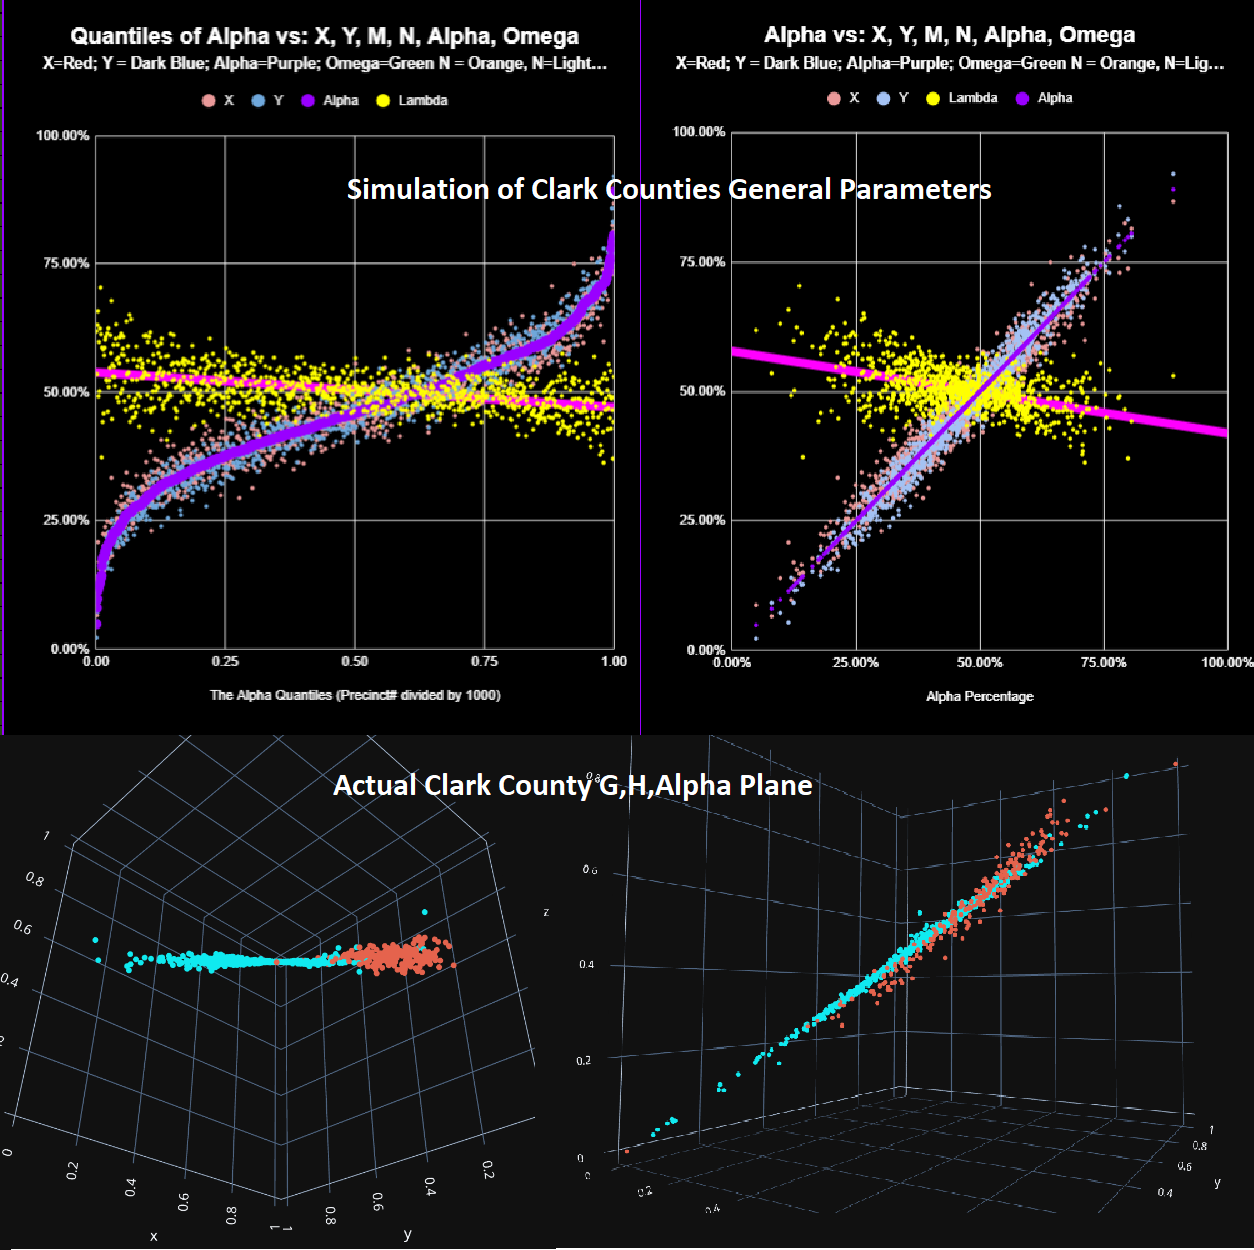
\includegraphics[width=225pt]{G,H,Alpha ClarkWashoe2004.png}}
\end{center}
\end{figure}
\newpage
\subsection{The Fair Election of 2008, Obama vs McCain, M Parallel to N}

Here is the link to the 2008 Election in Clark County: \url{https://docs.google.com/spreadsheets/d/132OMXgiCiU-f1tGrV5xdlLYoNgith6OTsftIQJZyAXU/edit?usp=sharing}.

Again, the wisdom of Little Johnny the Fifth Grader prevails, that the difference between $m$ and $n$ should be the same across the precincts, and with a little help from the academics, can be said that we expect $m$ to be parallel to $n$ (that is have the same general incline) since any inclination of either $m$ or $n$ must be due to non-political demographic factors, as the average distance between $m$ and $n$ is already accounted for by politically charged demographics.

The funny part is that I show them these graphs first, before the 2020 and 2022 graphs. It's fun to watch dishonest academics (Deceivers) try to wriggle their way out of the hole they dug and try to explain away constant lambda at 63.5\% with non sense terms like ``Mail-in Drift" or ``Partisan Enthusiasm" that they refuse to put in concrete mathematical terms for examination.

You see, the Laws of Geometry don't recognize for your woke feelings. The Twenty Laws and Forty Isometries are Eternal, Unyielding and Unforgiving.
\begin{figure}[bp!]
\begin{center}
\caption{$Y<X$ and $M<N$ (Parallel), 2008 Clark County}
\noindent\makebox[\textwidth]{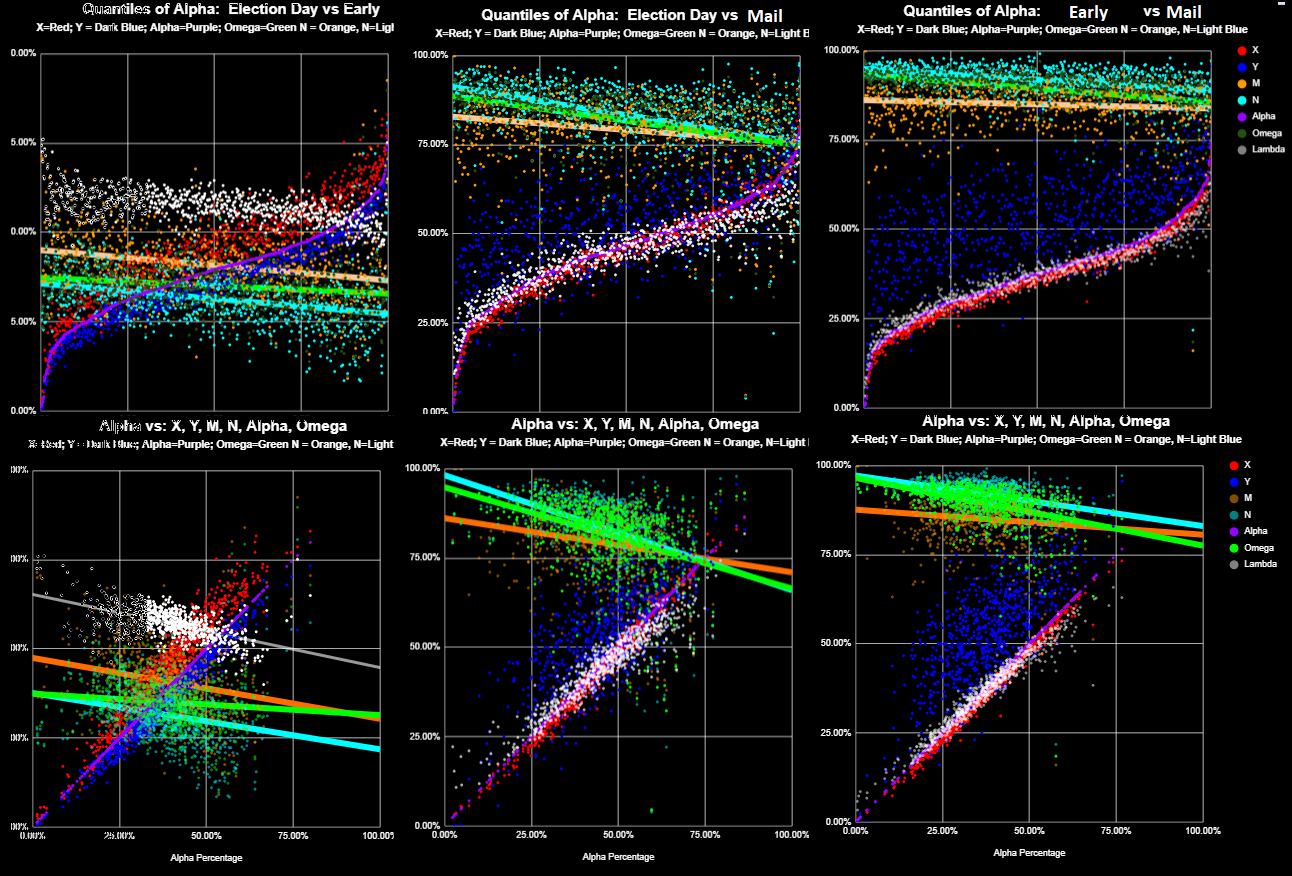
\includegraphics[width=400pt]{Clark 2008.png}}
\end{center}
\end{figure}
\newpage
\subsection{The Fair Election of 2012, Obama vs Romney, X=Y and M=N}

Here is the link to the 2012 Election in Clark County: \url{https://docs.google.com/spreadsheets/d/1ai1_Rjavj2razWUeE-nbDr1dr9kE5EV3UqOJO7K2qVE/edit?usp=sharing}.

In this election, $x=y$ and $m=n$ in all comparisons, that is for Election Day vs Early, Election Day vs Mail and Early vs Mail.

So far the historical precedent practically everywhere in the nation (not just Nevada) prior to 2012 is that $x=y$ and $m=n$ or otherwise parallel with a small offset.
\begin{figure}[bp!]
\begin{center}
\caption{$Y=X$ and $M=N$ (Parallel), 2012 Clark County}
\noindent\makebox[\textwidth]{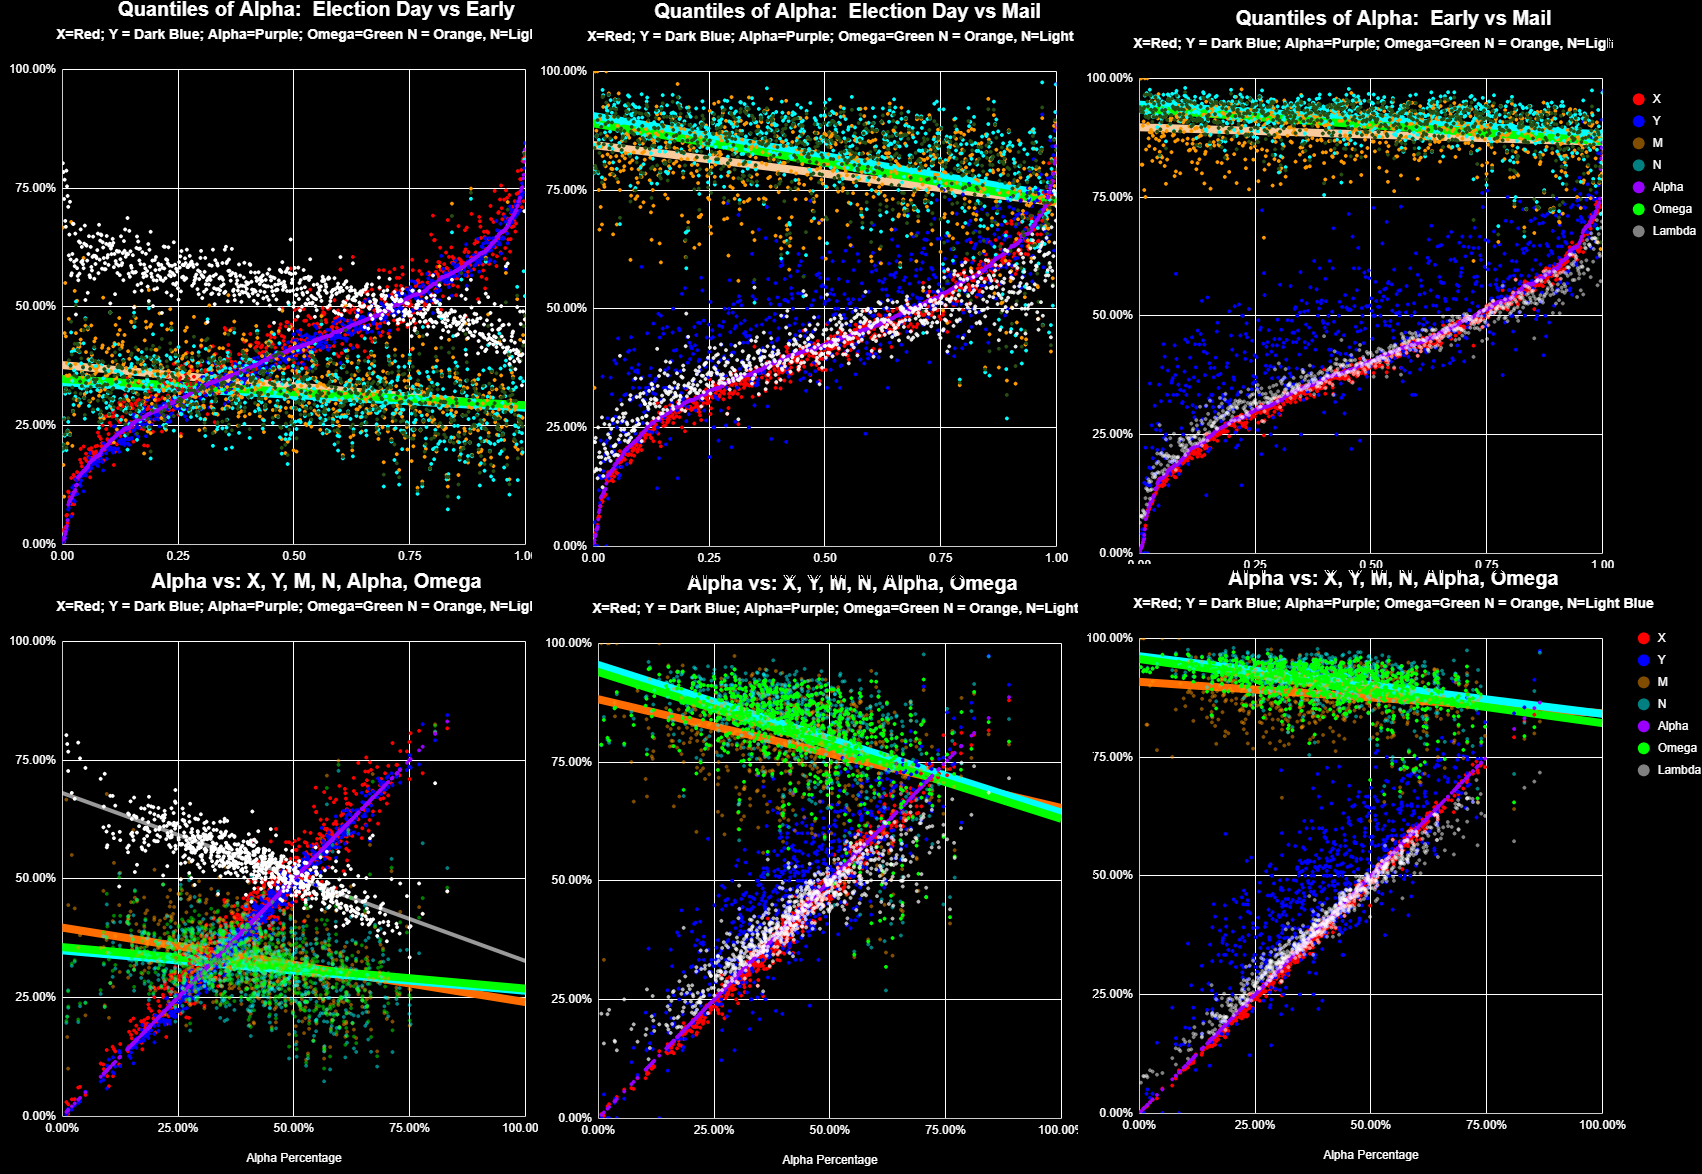
\includegraphics[width=400pt]{Clark 2012.png}}
\end{center}
\end{figure}
\newpage
\subsection{The Fair Election of 2016, Trump vs Hillary, X=Y and M=N}

Here is the link to the 2016 Election in Clark County: \url{https://docs.google.com/spreadsheets/d/1cKWHtQiGncMy13ep0d7TuMYPzWqpw_2setgwvIRBrMU/edit?usp=sharing}.

In this election, $x=y$ and $m=n$ in all comparisons, that is for Election Day vs Early, Election Day vs Mail and Early vs Mail.

So far the historical precedent practically everywhere in the nation (not just Nevada) prior to 2016 is that $x=y$ and $m=n$ or otherwise parallel with a small offset.

Of course, it all ends in 2020, with COVID-19 and mass mail-in ballots. The Twenty Laws and Forty Isometries Fail, the first victims of Covid! X diverges from Y and M diverges from N and Lambda acts as an Obstacle to Republican Victory in the General Election and an Obstacle to Patriots in Republican Primaries. Amazing times! And even long after 2020, the Twenty Laws and Forty Isometries remain dead. Now every casts their ballots while riding bivariate quaternionic cubic rollercoasters!
\begin{figure}[bp!]
\begin{center}
\caption{$Y=X$ and $M=N$ (Parallel), 2016 Clark County}
\noindent\makebox[\textwidth]{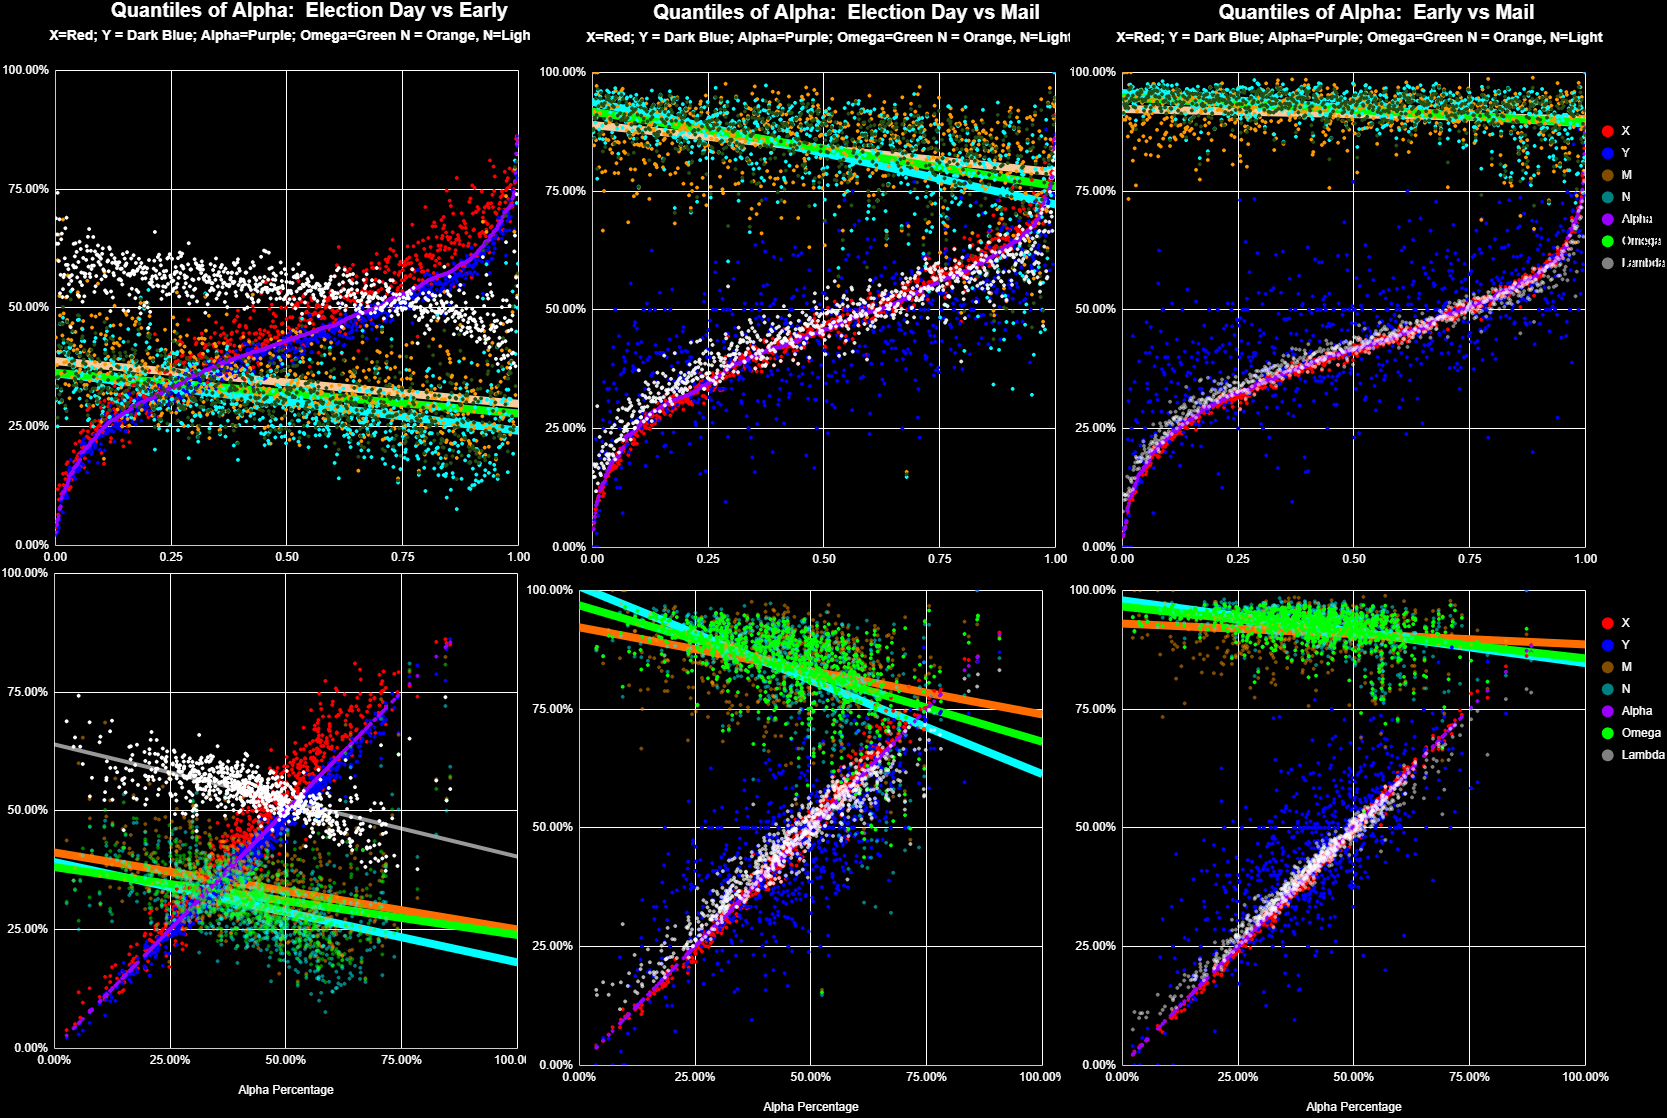
\includegraphics[width=400pt]{Clark 2016.png}}
\end{center}
\end{figure}
\newpage
\subsection{Brief Introduction to Complex Number Percentages and Manifolds for Two Simultaneous Races}

Just as the Linear Approximations of Biden's Mail-in Vote in terms of Total Ballots Cast and Trump's Early Vote are watered down explanations of the $g,h,\alpha$ manifolds in Nevada, so are the real number manifolds of $g,h,\alpha$ watered down versions of quaternionic $g,h,\alpha$ manifolds for the common mathematicians that doesn't deal with quaternions on a daily basis.

Since any quaternion can rewritten as a locally complex number (using the unit vector of its imaginary $i,j,k$ component), we will first start with the complex numbers themselves and how they apply to two races.

Suppose we have two candidates, a Republican and Democrat, for two races, the President and the Senate.

Alice and Bob are the Republican and Democrat candidates of the Presidential Race, and Cathy and Dan are the Republican and Democrat candidates of the Senate Race.

Before I state the vote total definitions, we do not recognize $a+bi$ as a complex number, rather we recognize $a\vec{q}+b\vec{i}$ as a complex number, where $\vec{q}$ is the $\vec{q}$ is the forward vector, $-\vec{q}$ is the reverse vector, $\vec{i}$ is the left vector and $-\vec{i}$ is the right vector. 

In elections we also don't use the word ``imaginary." The Senate Vote exists, even if we put an $\vec{i}$ next to it. The proper term for the $\vec{q}$ vector is the ``Forward Vector" and the proper term for $\vec{i}$ is the ``Lateral Vector."

We use the complex numbers for two races because the vote totals come from the same population of voters in each precinct. Thus, we cannot add them together as real numbers, but we can certainly treat them as complex numbers.
\newpage
Here are eight numbers for Early and Mail-in totals for Alice, Bob, Cathy and Dan.\\
Let $\vec{s}=214\vec{q}+189\vec{i}$ be Alice and Cathy's Early Vote.\\
Let $\vec{t}=244\vec{q}+251\vec{i}$ be Bob and Dan's Early Vote.\\
Let $\vec{u}=149\vec{q}+158\vec{i}$ be Alice and Cathy's Mail-in Vote.\\
Let $\vec{v}=229\vec{q}+209\vec{i}$ be Bob and Dan's Mail-in Vote.

$$\vec{x_{1}}=\frac{\vec{s}}{\vec{s}+\vec{t}}=0.4491\vec{q}-0.0188\vec{i}$$
$$\vec{y_{1}}=\frac{\vec{u}}{\vec{u}+\vec{v}}=0.4118\vec{q}+0.0181\vec{i}$$
$$\vec{\alpha_{1}}=\frac{\vec{s}+\vec{u}}{\vec{s}+\vec{t}+\vec{u}+\vec{v}}=0.4321\vec{q}-0.0021\vec{i}$$
$$\vec{\Omega_{1}}=\frac{\vec{s}+\vec{t}}{\vec{s}+\vec{t}+\vec{u}+\vec{v}}=0.5465\vec{q}-0.0013\vec{i}$$
$$(1-\vec{\Omega_{1}})=\vec{\Omega_{2}}=\frac{\vec{u}+\vec{v}}{\vec{s}+\vec{t}+\vec{u}+\vec{v}}=0.4535\vec{q}+0.0013\vec{i}$$

All of the Twenty Laws and Forty Isometries hold for the Complex Numbers, such as the Ninth Law (below). They also hold for the quaternions and the biquaternions, however we have to be careful from which side we multiply and divide from for the quaternions. For the complex numbers we need not worry about which side we multiply from, so we can apply them as written earlier in the chapter, such as:\\
The Ninth Law: $\vec{\alpha}=\vec{x}\vec{\Omega_{1}}+\vec{y}\vec{\Omega_{2}}$\\
The Ninth Law: $\vec{\alpha}=\vec{x}\cos^{2}( \vec\theta )+\vec{y}\sin^{2}( \vec\theta ); \cos(\vec{\theta})=+\sqrt{\Omega_{1}}; \sin(\vec{\theta})=+\sqrt{\Omega_{2}}$
$$1=\vec{\alpha_{1}}+\vec{\alpha_{2}}=\vec{\alpha_{1}}-\vec{i}^2\vec{\alpha_{2}}=\left(\vec{x_{1}}\cos^{2}( \vec\theta )+\vec{y_{1}}\sin^{2}( \vec\theta )\right)-\vec{i}^2\left(\vec{x_{2}}\cos^{2}( \vec\theta )+\vec{y_{2}}\sin^{2}( \vec\theta )\right)$$

The Complex Numbers also carry over the analogs of Convergence, Irrelevance and Twixt Lemmas, for instance the magnitude of $\vec{\alpha_{1}}$ must be between the magnitudes of $\vec{x_{1}}$ and $\vec{y_{1}}$, there is also a small rigid set of binary (logical) laws govern the bounds of the angular argument of $\vec{\alpha_{1}}$ based on the angular arguments and magnitudes of $\vec{\Omega_{1}}$, $\vec{x_{1}}$ and $\vec{y_{1}}$. Another example would be when the real number magnitude of $\Omega$ goes to zero or one, making one of the modes (Election Day or Mail) irrelevant, and making $\alpha$ converge upon $\vec{x_{1}}$ or $\vec{y_{1}}$ (whichever is the dominant mode).
\newpage
You can visit this link to interact with Alice's and Cathy's Complex Percentages: \url{https://docs.google.com/spreadsheets/d/14Bc64u1SeBrCL4Kp6DXz-c-1FsSRtQv97e5FZftvqWQ/edit?usp=sharing}. In the top-left graph, we see the $\vec{x_{1}}$ vector. Since the lateral component is mostly negative, it means that the Republican, Cathy for Senate, performed worse than Alice. Remember that since all of the integers of the election are positive, it means negative lateral components (and therefore negative angular arguments) will apportion more votes to Alice and less to Cathy in respect to the Real Number Magnitude of $\vec{x_{1}}$ (which you can see as the horizontal axis of the graph titled ``MagX vs MagY").

Likewise in the graph next to the top-left, we see the $\vec{y_{1}}$ vector. Cathy mysteriously does better than Alice in the Mail-in (since the lateral values are all positive). We can see the real number magnitude of $\vec{y_{1}}$ as the vertical axis of the graph ``MagX vs MagY." No matter how mysterious Cathy's mail-in energy may be, at least it's a random scatter plot. We won't be able to find a complex number manifold that predicts $\vec{\alpha_{1}}$ from $\vec{x_{1}}$ and $\vec{y_{1}}$ in this election.

To summarize a complex percentage: The Magnitude is the Strength of the Republican Vote, and the Angle is the distribution of the magnitude. As for the $\Omega$ percentage, in both a fair election and an election that is ``properly rigged" by a HVNN, the lateral component of $\Omega$ should be nigh zero, since we expect the same proportion of Early to Mail-in votes across the races at a precinct, and this expectation would be the Neural Network's most weighted cost function.
\begin{figure}[bp!]
\begin{center}
\caption{Alice and Beth's Complex Early, Mail-in and Aggregate Percentages}
\noindent\makebox[\textwidth]{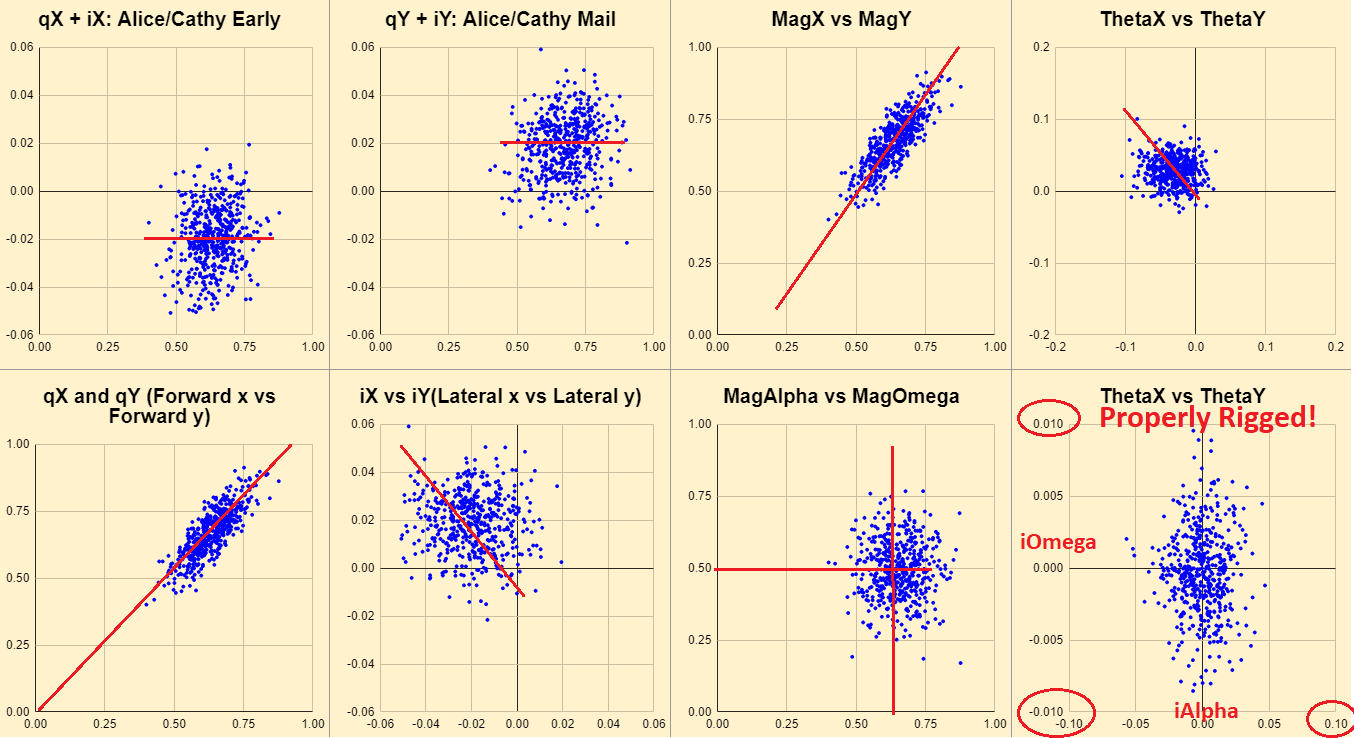
\includegraphics[width=425pt]{ComplexExample.png}}
\end{center}
\end{figure}
\newpage
In the Washoe 2020 Election, Trump received 114,574 votes, and Biden received 126,565 votes (thanks to the $\lambda$ Obstacle Percentage), a total of 241,138 ballots cast.

However, the Republican Amodei, for the Congressional House seat, received 119,663 votes (4000 more than Trump), and the Democrat Ackerman received 115,282 votes (11,000 less than Biden), a total of 234,954 ballots cast.

You are now going to see how this happened. It wasn't because of Trump's popularity amongst Republicans, it was because of a Complex Number Manifold that allows us to predict the Trump/Amodei complex aggregate percentage from the complex $g$ and $h$ percentages, even the exact value of the lateral part. 

It's amazing how Complex $\lambda$ was perfectly calibrated in these precincts to achieve this! You can see the below graphs identical in form to the graphs on the previous page in the Alice/Cathy vs Bob/Dan election; however, the graphs show the Complex West and East Side Percentages, instead of the Complex Early and Mail-in Percentages. Likewise the graphs show Complex Lambda instead of Complex Omega, since Lambda takes the place of Omega in the West vs East Orientation.

\begin{figure}[bp!]
\begin{center}
\caption{Trump's and Amodei's Complex West, East and Aggregate Percentages}
\noindent\makebox[\textwidth]{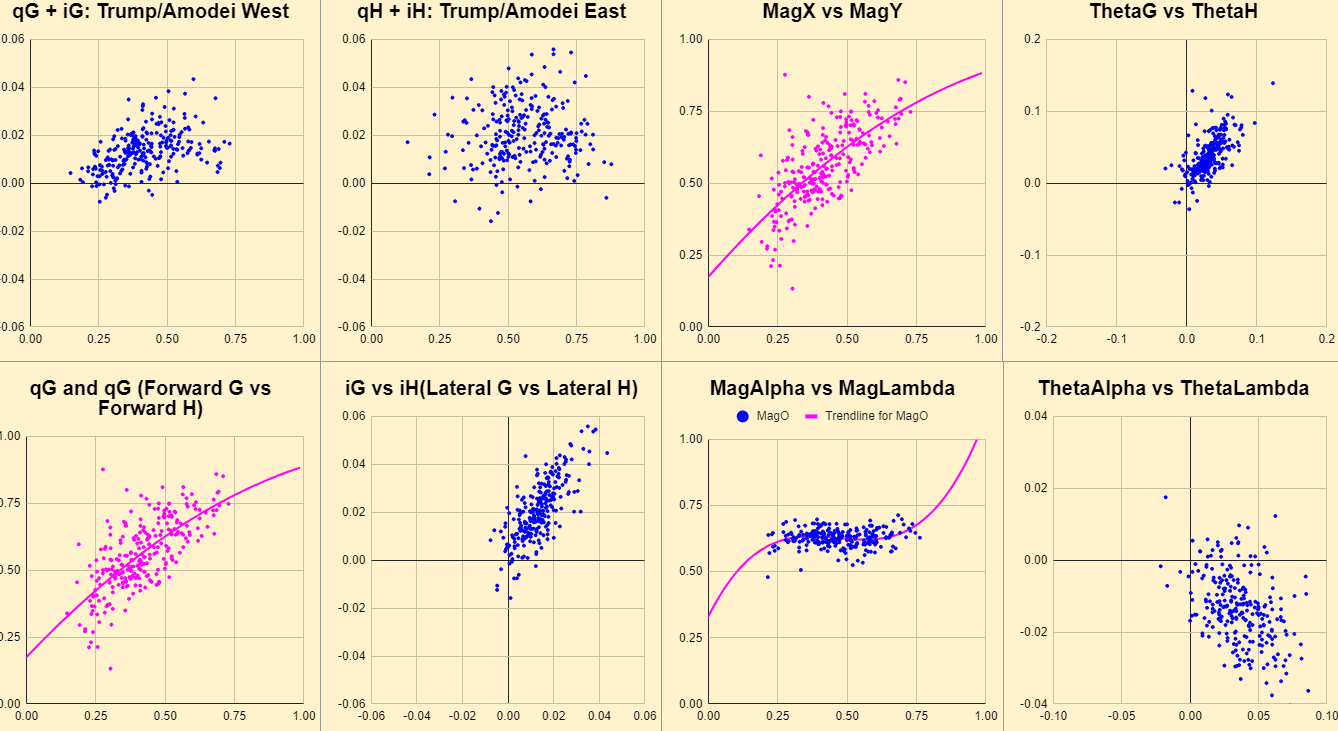
\includegraphics[width=425pt]{Washoe2020 TrumpAmodComplex.png}}
\end{center}
\end{figure}
\newpage
\subsection{The G,H,Alpha Complex Number Manifold That Rigged Trump/Amodei vs Biden/Ackermann in Washoe County}

You can see the results yourself here: \url{https://docs.google.com/spreadsheets/d/1W6ZHxeU3rrppg2cK12j-u7qzbWTNrsFm9BUO0NgUCJ8/edit?usp=sharing}

Vector Definitions:\\
Let $s_{1,b}$ and $s_{2,b}$ be Trump and Amodei's Early Vote at each $b^{th}$ precinct.\\
Let $t_{1,b}$ and $t_{2,b}$ be Biden and Ackerman's Early Vote at each $b^{th}$\\ precinct.
Let $u_{1,b}$ and $u_{2,b}$ be Trump and Amodei's Mail Vote at each $b^{th}$ precinct.\\
Let $v_{1,b}$ and $v_{2,b}$ be Biden and Ackerman's Mail Vote at each $b^{th}$ precinct.\\
Let $\vec{s_{b}}=s_{1,b}\vec{q}+s_{2,b}\vec{i}$ be the Republican Early Vote Vector at each $b^{th}$ precinct.\\
Let $\vec{t_{b}}=t_{1,b}\vec{q}+t_{2,b}\vec{i}$ be the Democrat Early Vote Vector at each $b^{th}$ precinct.\\
Let $\vec{u_{b}}=u_{1,b}\vec{q}+u_{2,b}\vec{i}$ be the Republican Mail-in Vote Vector at each $b^{th}$ precinct.\\
Let $\vec{v_{b}}=v_{1,b}\vec{q}+v_{2,b}\vec{i}$ be the Democrat Mail-in Vote Vector at each $b^{th}$ precinct.

Let $\vec{g_{b}}=\frac{\vec{s_{b}}}{\vec{s_{b}}+\vec{v_{b}}}$ be the Republican West Side Vector at each $b^{th}$ precinct.

Let $\vec{h_{b}}=\frac{\vec{u_{b}}}{\vec{u_{b}}+\vec{t_{b}}}$ be the Republican East Side Vector at each $b^{th}$ precinct.

Let $\vec{\alpha_{b}}=\frac{\vec{s_{b}}+\vec{u_{b}}}{\vec{s_{b}}+\vec{t_{b}}+\vec{u_{b}}+\vec{v_{b}}}$ be the Republican Aggregate at each $b^{th}$ precinct.

Then, with an $R^2=0.9982$ on the Entire Complex Value of $\vec{\alpha_{b}}$, with an $R^2=0.9920$ on the lateral part and an $R^2>0.999$ on the Forward Part, we have, in each precinct, the following Bivariate Complex Cubic Manifold of $\vec{\alpha_{b}}$ from $\vec{g_{b}}$ and $\vec{h_{b}}$:

$$\vec{\alpha_{b}}=\sum_{n=0}^{n=3}\left(\sum_{m=0}^{m=n}\left(\vec{c}_{n,m}\right)\left(\vec{g}_{b}^m\right)\left(\vec{h}_{b}^{(n-m)}\right) \right)$$
$$\vec{\alpha_{b}}=\vec{c}_{0,0}+\vec{c}_{1,0}\vec{h_{b}}+\vec{c}_{1,1}\vec{g_{b}}+\vec{c}_{2,0}\vec{h_{b}}^2+\vec{c}_{2,1}\vec{g_{b}}\vec{h_{b}}+\vec{c}_{2,2}\vec{g_{b}}^2+\vec{c}_{3,0}\vec{h_{b}}^3+\vec{c}_{3,1}\vec{g_{b}}\vec{h_{b}}^2+\vec{c}_{3,2}\vec{g_{b}}^2\vec{h_{b}}+\vec{c}_{3,3}\vec{g_{b}}^3$$

Table of Complex Constants:\\
$\vec{c}_{0,0}=+0.0050031\vec{q}+0.0007984\vec{i}$, $\vec{c}_{1,0}=+0.4566745\vec{q}+0.0035635\vec{i}$\\
$\vec{c}_{1,1}=+0.4857910\vec{q}-0.0121609\vec{i}$, $\vec{c}_{2,0}=-0.68558265\vec{q}-0.05195035\vec{i}$\\
$\vec{c}_{2,1}=+1.2112560\vec{q}+0.1520030\vec{i}$, $\vec{c}_{2,2}=-0.3562887\vec{q}-0.0821964\vec{i}$\\
$\vec{c}_{3,0}=+0.8313736\vec{q}+0.0490390\vec{i}$, $\vec{c}_{3,1}=-1.5365175\vec{q}-0.0488619\vec{i}$\\
$\vec{c}_{3,2}=+0.6192315\vec{q}-0.1203566\vec{i}$, $\vec{c}_{3,3}=-0.0622280\vec{q}+0.1115814\vec{i}$
\newpage
In the top series of graphs you see the integer returns of Trump's and Amodei's Total Vote by multiplying the Expected Complex Aggregate from the $g,h$ complex cubic manifold, against the Total Number (complex number) of ballots cast at the precinct in the Presidential and House Race. We yield $R^2=.99999$ on both total votes, with a mean error less than 0.01 vote with the standard deviation of the error being less than 4 votes. 

In the bottom series of graphs you see the result of the expected Forward Part vs the actual Forward Part of Complex Alpha, and the expected Lateral Part vs the actual Lateral Part. Finally you see the Complex Residuals of the Alpha Vector. I had to zoom in 100x in order for you to see them! Thus, we know the exact magnitude and the exact angular distribution of Trump's and Amodei's votes in each precinct, without ever knowing the complex value of $\lambda$.
\begin{figure}[bp!]
\begin{center}
\caption{The Extraordinary Precision of the Bivariate Complex Cubic Manifold}
\noindent\makebox[\textwidth]{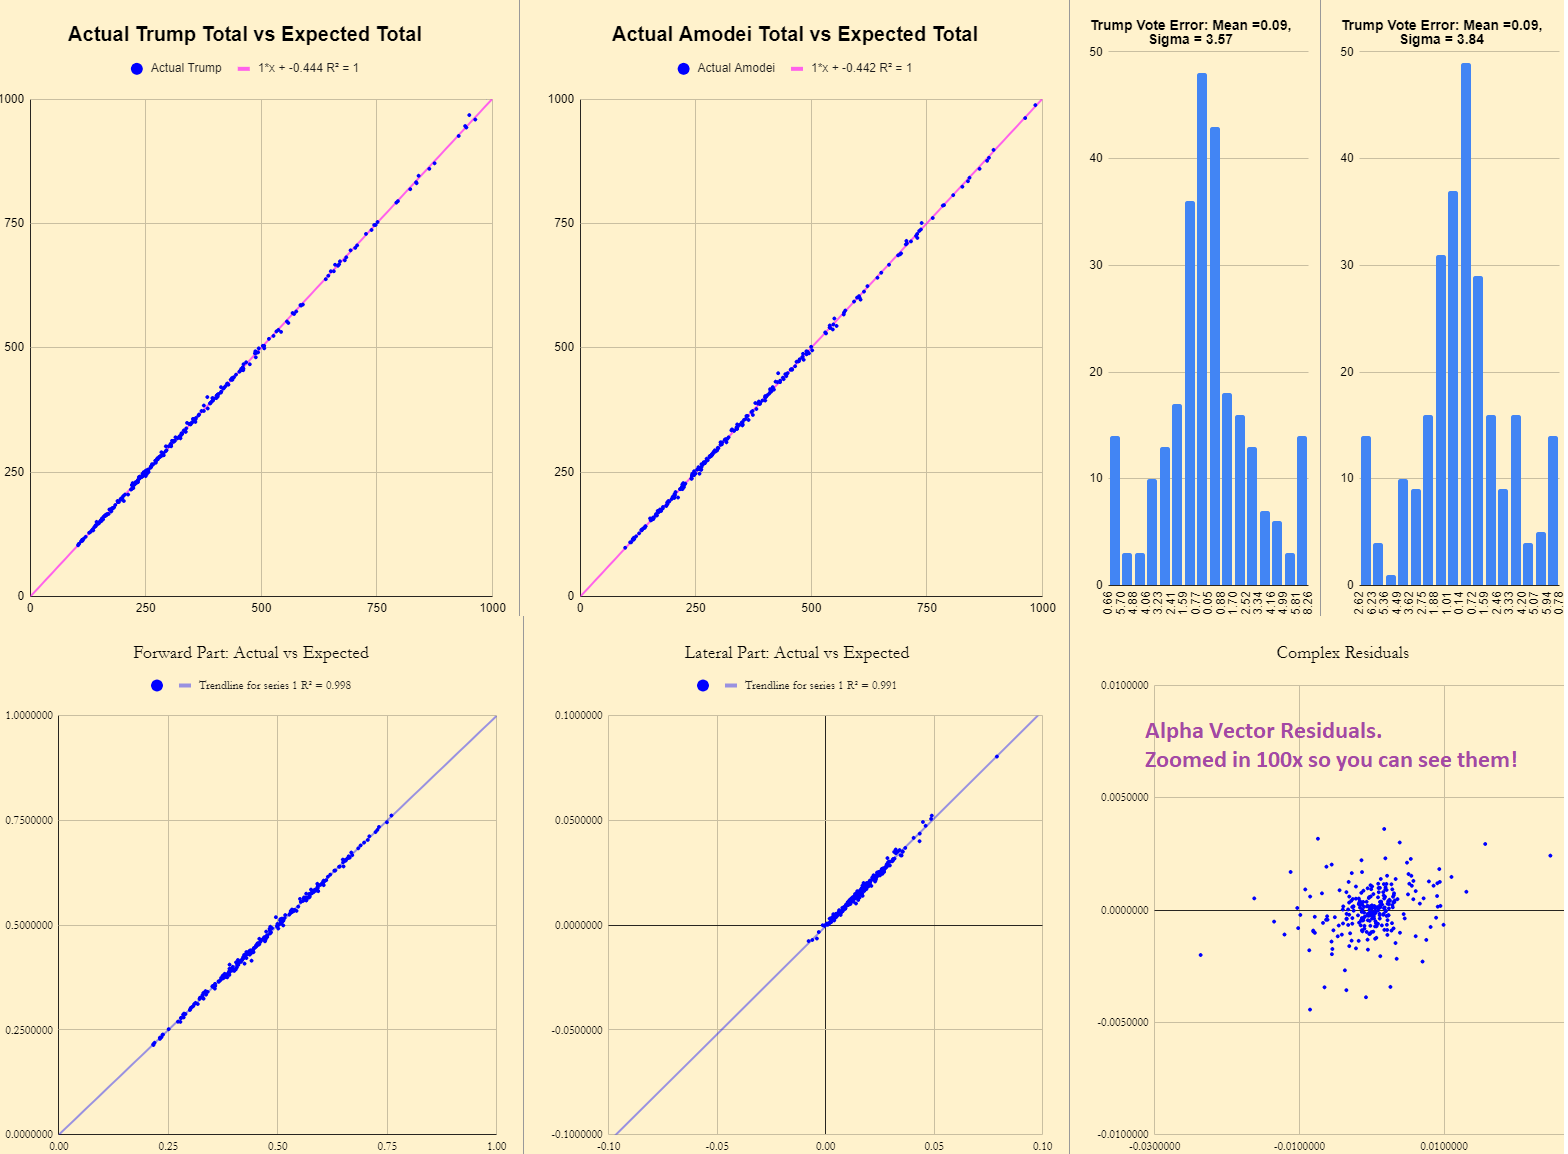
\includegraphics[width=450pt]{ComplexManifoldResult.png}}
\end{center}
\end{figure}
\newpage
\subsection{Brief Introduction to Quaternionic Percentages and Manifolds for Four Simultaneous Races}
For the quaternions we need define left and right handed multiplication in a manner that upholds the Twenty Laws and Forty Isometries. We can use the real/complex numbers as a guide. Let's take a look at the Ninth Law for the reals/complex numbers, where $\vec{z}$ is the total ballots cast:

$$\vec{\alpha}_{1}=\vec{x}_{1}\vec{\Omega}_{1}+\vec{y}_{1}\vec{\Omega}_{2}=\vec{s}\left((\vec{s}+\vec{t})^{-1}\right)(\vec{s}+\vec{t})\left(\vec{z}\right)^{-1}+\vec{u}\left((\vec{u}+\vec{v})^{-1}\right)(\vec{u}+\vec{v})\left(\vec{z}\right)^{-1}=\left(\vec{s}+\vec{u}\right)\left(\vec{z}\right)^{-1}$$

Using the same ordering of left to right multiplication, the above formula will hold for the quaternions. 

Thus, we define the vector percentages as:
$$\vec{x}_{1,b}=\vec{s}_{b}\left(\frac{1}{\vec{s}_{b}+\vec{t}_{b}}\right); \vec{\Omega}_{1,b}=\left(\vec{s}_{b}+\vec{t}_{b}\right)\left(\frac{1}{\vec{z}_{b}}\right); \vec{y}_{1,b}=\vec{u_{b}}\left(\frac{1}{\vec{u}_{b}+\vec{v}_{b}}\right); \vec{\Omega}_{2,b}=\left(\vec{u_{b}}+\vec{v_{b}}\right)\left(\frac{1}{\vec{z}_{b}}\right)$$

Where $\vec{s}_{b}=s_{1,b}\vec{q}+s_{2,b}\vec{i}+s_{3,b}\vec{j}+s_{4,b}\vec{k}$, which are the Early Vote Totals for the four Republican Nominees at each $b^{th}$ precinct.

$\vec{t}_{b}=t_{1,b}\vec{q}+t_{2,b}\vec{i}+t_{3,b}\vec{j}+t_{4,b}\vec{k}$, which are the Early Vote Totals for the four Democrat Nominees in four races at each $b^{th}$ precinct.

$\vec{u}_{b}=u_{1,b}\vec{q}+u_{2,b}\vec{i}+u_{3,b}\vec{j}+u_{4,b}\vec{k}$, which are the Mail-in Totals for the four Republican Nominees in four races at each $b^{th}$ precinct.

$\vec{v}_{b}=v_{1,b}\vec{q}+v_{2,b}\vec{i}+v_{3,b}\vec{j}+v_{4,b}\vec{k}$, which are the Mail-in Totals for the four Democrat Nominees in four races at each $b^{th}$ precinct.

$\vec{z}_{b}=\vec{s}_{b}+\vec{t}_{b}+\vec{u}_{b}+\vec{v}_{b}$ at each $b^{th}$ precinct.

Just as the angle of the complex number aggregate determines the distribution of the alpha vector magnitude between both nominees of the same party in two races, so do the angles of the quaternionic aggregate determine the distribution of the alpha vector magnitude to the four nominees of the same party in four races.
\newpage
We can rewrite the quaternion,$\vec{\alpha}_{1,b}$ , as:
$$\vec{\alpha}_{1,b}=a_{0,b}\vec{q}+a_{1,b}\vec{i}+a_{2,b}\vec{j}+a_{3,b}\vec{k}=a_{0,b}\vec{q}+w_{b}\vec{\Lambda}_{b}=M_b\left(\vec{q}\cos(\theta_b)+\vec{\Lambda}_{b}\sin(\theta_b)\right)$$
$$M_{b}=\sqrt{a_{0,b}^2+a_{1,b}^2+a_{2,b}^2+a_{3,b}^2}; \vec{\Lambda}_{b}=\frac{a_{1,b}\vec{i}+a_{2,b}\vec{j}+a_{3,b}\vec{j}}{\sqrt{a_{1,b}^2+a_{2,b}^2+a_{3,b}^2}}; \theta_{b}=ATAN2\left(\frac{\sqrt{a_{1,b}^2+a_{2,b}^2+a_{3,b}^2}}{a_{0,b}}\right )$$
Where $M_{b}$ is the magnitude of the alpha vector, $\vec{\Lambda}_{b}$ is the direction of the vector in $i,j,k$ space and $\theta_{b}$ is the relationship between the first candidate and the other three candidates, a perfect system to ensure that the Republican, Lombardo, wins the the Gubernatorial Race (who stole the Republican primary from Gilbert), while his three Republican nominees lose down the ballot.

However, since Mother Nature doesn't have four-quadrant arctangent function or a Magnitude Function (nor does she need them), the correct way to write the alpha vector (in manner that holds for the Biquaternions), is as follows (the angle, $\theta_{b}$, is a complex number for the Biquaterions:
$$\vec{\alpha}_{1,b}=a_{0,b}\vec{q}+w_{b}\vec{\Lambda}_{b}=a_{0,b}\sec{\theta_b}\left(\vec{q}\cos{\theta_b}+\vec{\Lambda}_b\sin{\theta_b}\right); \theta_{b}=\arctan{\frac{w_{b}}{a_{0,b}}}$$
$$w_{b}=\sqrt{-\left({a_{1,b}\vec{i}}+{a_{2,b}\vec{j}}+{a_{3,b}\vec{k}}\right)\left({a_{1,b}\vec{i}}+{a_{2,b}\vec{j}}+{a_{3,b}\vec{k}}\right)}=\sqrt{a_{1,b}^2+a_{2,b}^2+a_{3,b}^2}$$

Notice that the only the regular Arctangent is used in the above formulation.
\newpage
We can see this also holds for the complex numbers, which are a subset of the biquaternions. For the below equation $\vec{\theta}$ is a complex angle, describing an affine basis of non-unit vectors, and $\phi$ is a real number angle, describing only a rotation of the existing affine basis, with the magnitude of $\vec{z}$, $Z$, scaling the entire rotated affine basis at the end.

This form easily allows us to find the reciprocal and the $m^{th}$ root of $n$ unity for any complex number, quaternion or biquaternion, and therefore allows us to do Complex, Quaternionic and Biquaternionic Least Squares for two, four or eight rigged races at a time.  It also allows you to simply the existing equations of Weyl Spinors and other quaterionic entities in the physical sciences!
$$\vec{a}\vec{q}+\vec{b}\vec{i}=\vec{a}\sec(\vec{\theta})\left(\vec{q}\cos{\vec{\theta}+\vec{i}\sin{\vec{\theta}}}\right)=\vec{z}\left(e^{\vec{\theta}}\right)=Z\left(e^{\vec{i}\phi}\right)\left(e^{\vec{\theta}}\right)=\left(e^{\vec{\theta}+\vec{i}\left(\phi-\vec{i}\ln{Z}\right)}\right); \vec{\theta}=\arctan\left(\frac{\vec{b}}{\vec{a}}\right)$$
$$\vec{z}=\vec{a}\sec(\vec{\theta})=z_{0}\vec{q}+z_{1}\vec{i}=z_{0}\sec(\phi)\left(\vec{q}cos{\phi}+\vec{i}\sin(\phi)\right); \phi=\arctan\left(\frac{z_{1}}{z_{0}}\right); Z=\sqrt{\left(z_{0}\vec{q}+z_{1}\vec{i}\right)\left(z_{0}\vec{q}-z_{1}\vec{i}\right)}$$
Hence we can write any biquaterion, using $\vec{w}$ as the immediate lateral vector to $\vec{q}$ that commutes with $i,j,k$, as:
$$\vec{a}\vec{q}+\vec{b}\vec{\Lambda}=\left(\sqrt{\left(z_0\vec{q}+z_{1}\vec{w}\right)\left(z_0\vec{q}-z_{1}\vec{w}\right)}\right)\left(\vec{q}\cos(\phi)+\vec{w}\sin(\phi)\right)\left(\vec{q}cos{\vec{\theta}}+\vec{\Lambda}\sin{\vec{\theta}}\right)$$
Thus the reciprocal of a biquaternion is given as:
$$\left(\vec{a}\vec{q}+\vec{b}\vec{\Lambda}\right)^{-1}=\left(\sqrt[-2]{\left(z_0\vec{q}+z_{1}\vec{w}\right)\left(z_0\vec{q}-z_{1}\vec{w}\right)}\right)\left(\vec{q}\cos(-\phi)+\vec{w}\sin(-\phi)\right)\left(\vec{q}cos{(-\vec{\theta})}+\vec{\Lambda}\sin{(-\vec{\theta})}\right)$$
And the Mth Root of N unity, $\sqrt[m,n]{\left(\vec{a}\vec{q}+\vec{b}\vec{\Lambda}\right)}$, is given by:
$$\left(\sqrt[-2n]{\left(z_0\vec{q}+z_{1}\vec{w}\right)\left(z_0\vec{q}-z_{1}\vec{w}\right)}\right)
\left(\vec{q}\cos\left(\frac{\phi+2m\pi}{n}\right)+\vec{w}\sin\left(\frac{\phi+2m\pi}{n}\right)\right)
\left(\vec{q}cos{\left(\frac{1}{n}\vec{\theta}\right)}+\vec{\Lambda}\sin{\left(\frac{1}{n}\vec{\theta}\right)}\right)$$

It pains me to say that I have pioneered the depths of Hypercomplex Numbers to save my country from Election Fraud, rather than to advance the knowledge and potential of mankind through the sciences and generalized data analysis (such as hypercomplex market analysis). Alas, it is so, and it had to be done to save us all from Hypercomplex-Valued Neural Networks rigging our elections.

For now we shall stick with the regular quaternions for Nevada, since Biquaternions aren't needed here (they rig eight elections at a time with Biquaternions in Will County Illinois).
\newpage
\subsection{The Quaternionic Manifold of the Nevada 2022 General Election that allowed Lombardo to win while making the other Republicans lose.}

For the Gubernatorial Race (Lombardo vs Sisolak), Secretary of State Race (Marchant vs Cisco), Attorney General's Race (Sigal vs Ford) and the Secretary of Treasury's Race (Fiore vs Conine), with an $R^2=0.9985$, there exists a quaternionic manifold of the West, East and Aggregate Percentages of the Republicans (Lombard, Marchant, Sigal, and Fiore), let allows us to solve for anyone of the $g,h,\alpha$ vectors, knowing the other two, with no knowledge of the quaternionic value of $\lambda$.

Vote Total Definitions; For each $b^{th}$ precinct let:\\
$p_{(0,0,b)}, p_{(0,1,b)}, p_{(0,2,b)}$ be Lombardo's Early, Mail and Election Day Votes.\\
$p_{(1,0,b)}, p_{(1,1,b)}, p_{(1,2,b)}$ be Sisolak's Early, Mail and Election Day Votes.\\
$p_{(2,0,b)}, p_{(2,1,b)}, p_{(2,2,b)}$ be Marchant's Early, Mail and Election Day Votes.\\
$p_{(3,0,b)}, p_{(3,1,b)}, p_{(3,2,b)}$ be Cicso's Early, Mail and Election Day Votes.\\
$p_{(4,0,b)}, p_{(4,1,b)}, p_{(4,2,b)}$ be Sigal's Early, Mail and Election Day Votes.\\
$p_{(5,0,b)}, p_{(5,1,b)}, p_{(5,2,b)}$ be Ford's Early, Mail and Election Day Votes.\\
$p_{(6,0,b)}, p_{(6,1,b)}, p_{(6,2,b)}$ be Fiore's Early, Mail and Election Day Votes.\\
$p_{(7,0,b)}, p_{(7,1,b)}, p_{(7,2,b)}$ be Conine's Early, Mail and Election Day Votes.\\

The $\vec{s}_b$ precinct vectors are the sum of the Republican Early Vote and Election Day Vote in each precinct, for each race, as follows:\\
$s_{1}=p_{(0,0,b)}+p_{(0,2,b)}; s_{2}=p_{(2,0,b)}+p_{(2,2,b)};\\
s_{3}=p_{(4,0,b)}+p_{(4,2,b)}; s_{4}=p_{(6,0,b)}+p_{(6,2,b)}$; $\vec{s}_{b}=s_{1}\vec{q}+s_{2}\vec{i}+s_{3}\vec{j}+s_{4}\vec{k}$

The $\vec{t}_b$ precinct vectors are the sum of the Democrat Early Vote and Election Day Vote in each precinct, for each race, as follows:\\
$t_{1}=p_{(1,0,b)}+p_{(1,2,b)}; t_{2}=p_{(3,0,b)}+p_{(3,2,b)};\\
t_{3}=p_{(5,0,b)}+p_{(5,2,b)}; t_{4}=p_{(7,0,b)}+p_{(7,2,b)}$; $\vec{t}_{b}=t_{1}\vec{q}+t_{2}\vec{i}+t_{3}\vec{j}+t_{4}\vec{k}$

The $\vec{u}_b$ precinct vectors are the Republican Mail-in Vote in precinct, for each race, as follows:\\
$u_{1}=p_{(0,1,b)}; s_{2}=p_{(2,1,b)}; u_{3}=p_{(4,2,b)}; u_{4}=p_{(6,1,b)}$; $\vec{u}_{b}=u_{1}\vec{q}+u_{2}\vec{i}+u_{3}\vec{j}+u_{4}\vec{k}$

The $\vec{v}_b$ precinct vectors are the Democrat Mail-in Vote in precinct, for each race, as follows:\\
$v_{1}=p_{(1,1,b)}; v_{2}=p_{(3,1,b)}; v_{3}=p_{(5,2,b)}; v_{4}=p_{(7,1,b)}$; $\vec{v}_{b}=v_{1}\vec{q}+v_{2}\vec{i}+v_{3}\vec{j}+v_{4}\vec{k}$
\newpage
The West Side Total Vector of each precinct is the total number of Republican Early, Republican Election Day and Democrat Mail-in Votes for each $b^{th}$ precinct, in each race, and is defined as follows:
$$\vec{c}_{b}=\vec{s}_{b}+\vec{v}_{b}$$

The East Side Total Vector of each precinct is the total number of Democrat Early, Democrat Election Day and Republican Mail-in Votes for each $b^{th}$ precinct, in each race, and is defined as follows:
$$\vec{d}_{b}=\vec{u}_{b}+\vec{t}_{b}$$

The Republican Total Vector of each precinct is the total number of Republican Early, Republican Election Day and Republican Mail-in Votes for each $b^{th}$ precinct, in each race, and is defined as follows:
$$\vec{f}_{b}=\vec{s}_{b}+\vec{u}_{b}$$

The Grand Total Vector of each precinct is the total number of all Early, all Election Day and all Mail-in Votes for each $b^{th}$ precinct, in each race, and is defined as follows:
$$\vec{z}_{b}=\vec{s}_{b}+\vec{t}_{b}+\vec{u}_{b}+\vec{v}_{b}$$

The West, East, Republican Aggregate and West Side Vertical Aggregate Percentages are defined as follows (and the multiplication of the numerators must executed explicitly from left to right as written):
$$\vec{g}_{b}=\left(\vec{s}_{b}\right)\left(\frac{1}{\vec{c}_{b}}\right); \vec{h}_{b}=\left(\vec{u}_{b}\right)\left(\frac{1}{\vec{d}_{b}}\right);
\vec{\alpha}_{b}=\left(\vec{f}_{b}\right)\left(\frac{1}{\vec{z}_{b}}\right);
\vec{\lambda}_{b}=\left(\vec{c}_{b}\right)\left(\frac{1}{\vec{z}_{b}}\right)$$

In a fair election, $\vec{\alpha}_{b}=\vec{g}_{b}\vec{\lambda}_{b}+\vec{h}_{b}\left(1\vec{q}-\vec{\lambda}_{b}\right)$; however, we can solve for either $\vec{\alpha}_{b}, \vec{g}_{b}$ or $\vec{h_{b}}$ from the other two, with no knowledge of $\vec{\lambda}_{b}$. This is the most grievous violation of the Twenty Laws and Forty Isometries ever witnessed.
\newpage
The Quadratic Quaternionic Manifold Equation is as follows:
$$\vec{\alpha}_b=\vec{c}_{0}+\vec{g}_{b}\vec{c}_{1}+\vec{h}_{b}\vec{c}_{2}+\vec{g}_{b}\vec{c}_{3}\vec{g}_{b}+\vec{g}_{b}\vec{c}_{4}\vec{h}_{b}+\vec{h}_{b}\vec{c}_{5}\vec{g}_{b}+\vec{h}_{b}\vec{c}_{6}\vec{h}_{b}$$
Table of Quaternionic Vectors Constants:\\
$\vec{c}_{0}=+0.00274199\vec{q}-0.00029744\vec{i}-0.00019403\vec{j}+0.00004472\vec{k}$\\
$\vec{c}_{1}=+0.54474612\vec{q}+0.00130453\vec{i}-0.00187845\vec{j}-0.00061189\vec{k}$\\
$\vec{c}_{2}=0.42897369\vec{q}-0.00021540\vec{i}+0.00277653\vec{j}+0.00047378\vec{k}$\\
$\vec{c}_{3}=+0.15316135\vec{q}-0.02206823\vec{i}-0.00877376\vec{j}+0.00492293\vec{k}$\\
$\vec{c}_{4}=+0.11747404\vec{q}+0.02979109\vec{i}+0.02175914\vec{j}-0.00575878\vec{k}$\\
$\vec{c}_{5}=-0.25345457\vec{q}+0.01928529\vec{i}+0.00481058\vec{j}-0.00798310\vec{k}$\\
$\vec{c}_{6}=+0.02733489\vec{q}-0.02603547\vec{i}-0.01739928\vec{j}+0.00866069\vec{k}$

\textcolor{red}{Remember that the precincts, from two distant counties on opposite sides of the State Nevada, Clark and Washoe, both voted identically upon the same quaternionic manifold!!! No one, not even the most woke academics, can find an answer for this! The Quaternionic Obstacle Percentage, $\vec{\lambda}_{b}$, is mighty here!}

Link the Calculator used to Reverse Engineer the Quaternionic Rig of Nevada 2022:
\url{https://docs.google.com/spreadsheets/d/1sz5axYMVkMichZ6aBW36O-JLXt4bakNvdGoRTpMruxA/edit?usp=sharing}

Link to the Scatter Plot of the Actual $i,j,k$ parts (blue) to the expected $i,j,k$ parts (red):\\
\url{https://plotly.com/~EKSolomon/108/}

A Quadratic Equation over the Quaternions is equivalent to four cubic equations over the real numbers. This is why all the $g,h,\alpha$ manifolds in 2020 and 2022 across the United States have significant cubic curvature when only looking at a single race (real numbers). You can learn how to perform quaternionic least squares and solve the quadratic equation for the quaternions here:

Video Link to my speech at the JMM2023 Conference, January 7th, 2023 on the General Solution to Quaternionic Least Squares:\\
\url{https://youtu.be/FOhWGq9KExE}

Full Paper of Quaternionic Least Squares:\\
\url{https://docs.google.com/document/d/1cbLQk2yIRvblb3T6odCmpk2QcGwpEEEqtuzjvMHkkW0/edit?usp=sharing}

Video Lecture on the derivation of the Quadratic Equation:\\
\url{https://www.youtube.com/live/UXKxMv39V0M?feature=share}

Quadratic Equation:\\
\url{https://docs.google.com/document/d/1dqnzOfj8I6f4zVrXB6ZnMXfwzA532N00P4qA31_y60U/edit?usp=sharing}
\begin{figure}[bp!]
\begin{center}
\caption{The Ghastly Precision of the Bivariate Quaternionic Manifold}
\noindent\makebox[\textwidth]{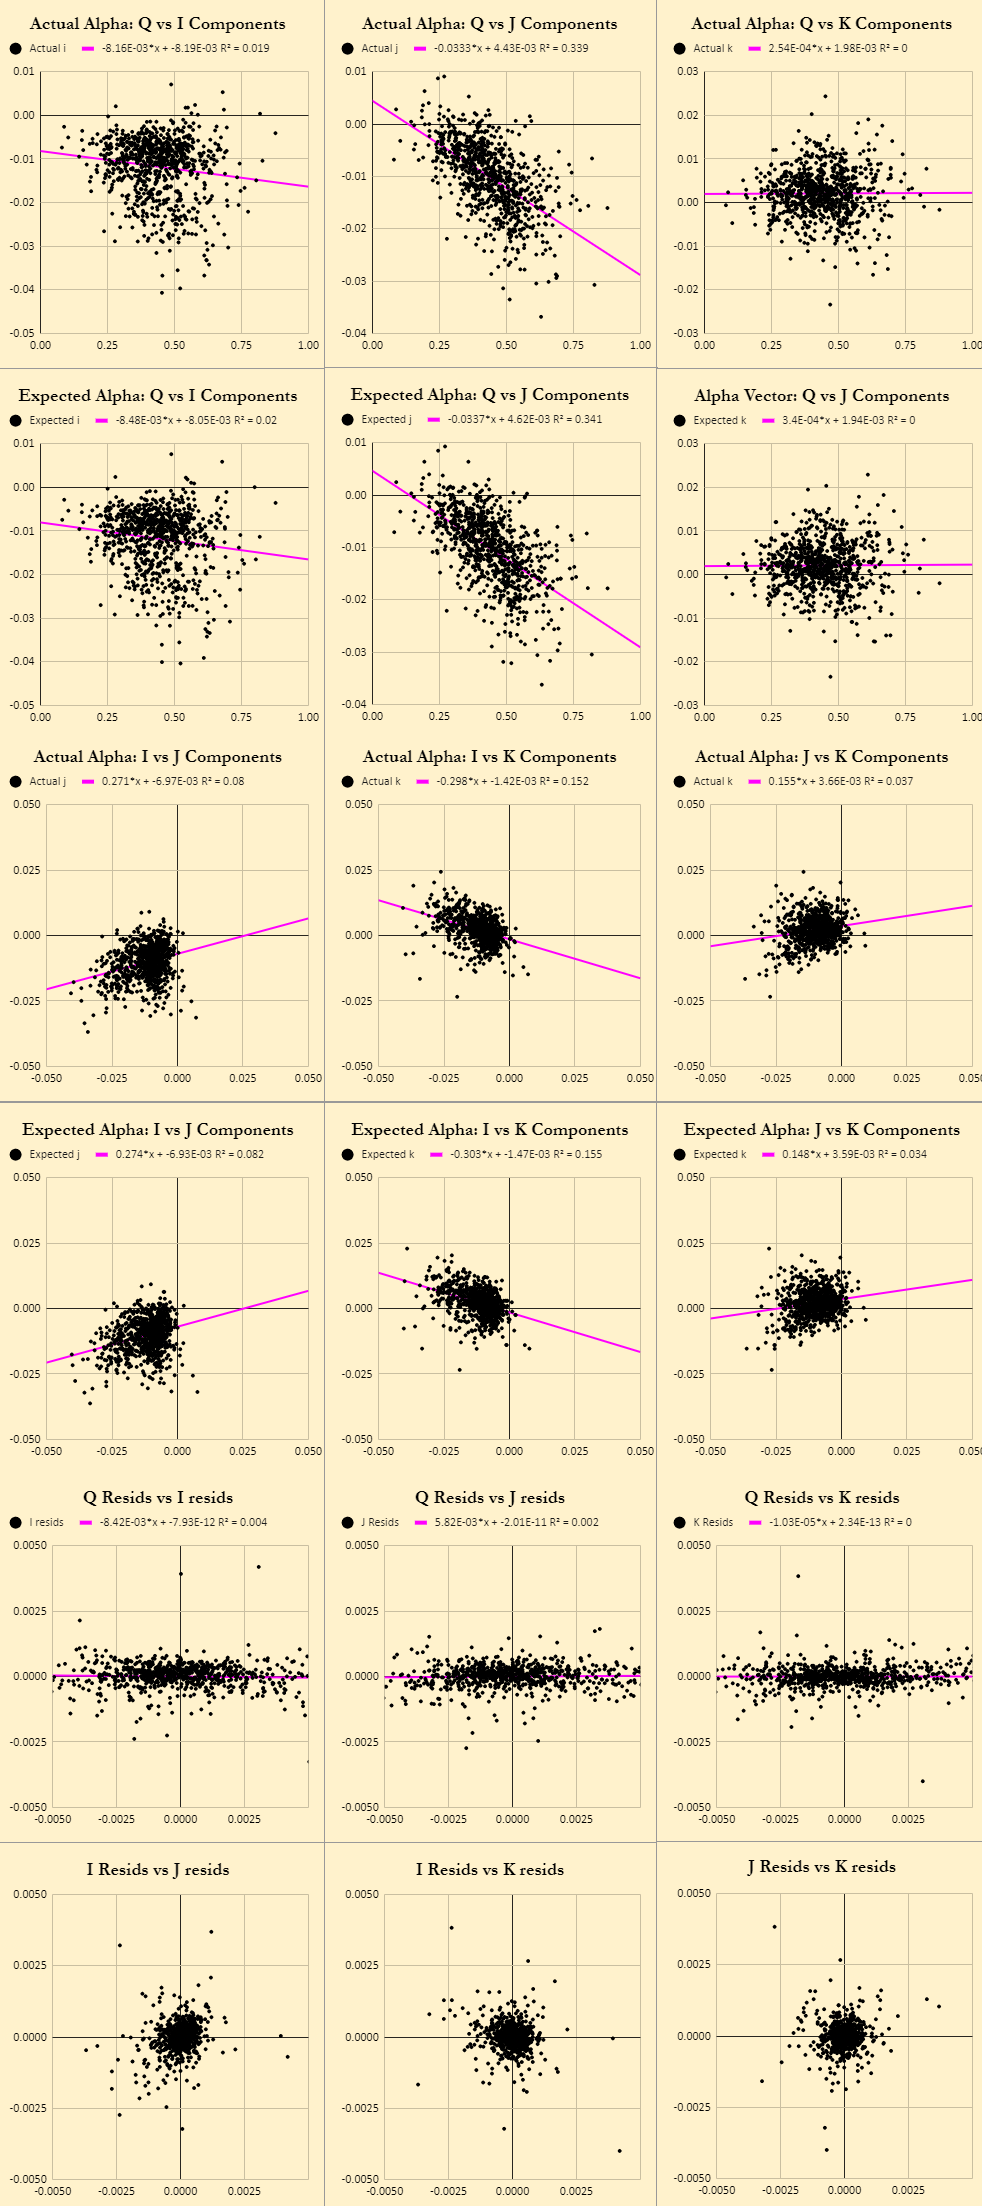
\includegraphics[width=350pt]{Quaterionic Results.png}}
\end{center}
\end{figure}
\begin{figure}[bp!]
\begin{center}
\caption{The Eerie Precision of the Republican Vote Totals}
\noindent\makebox[\textwidth]{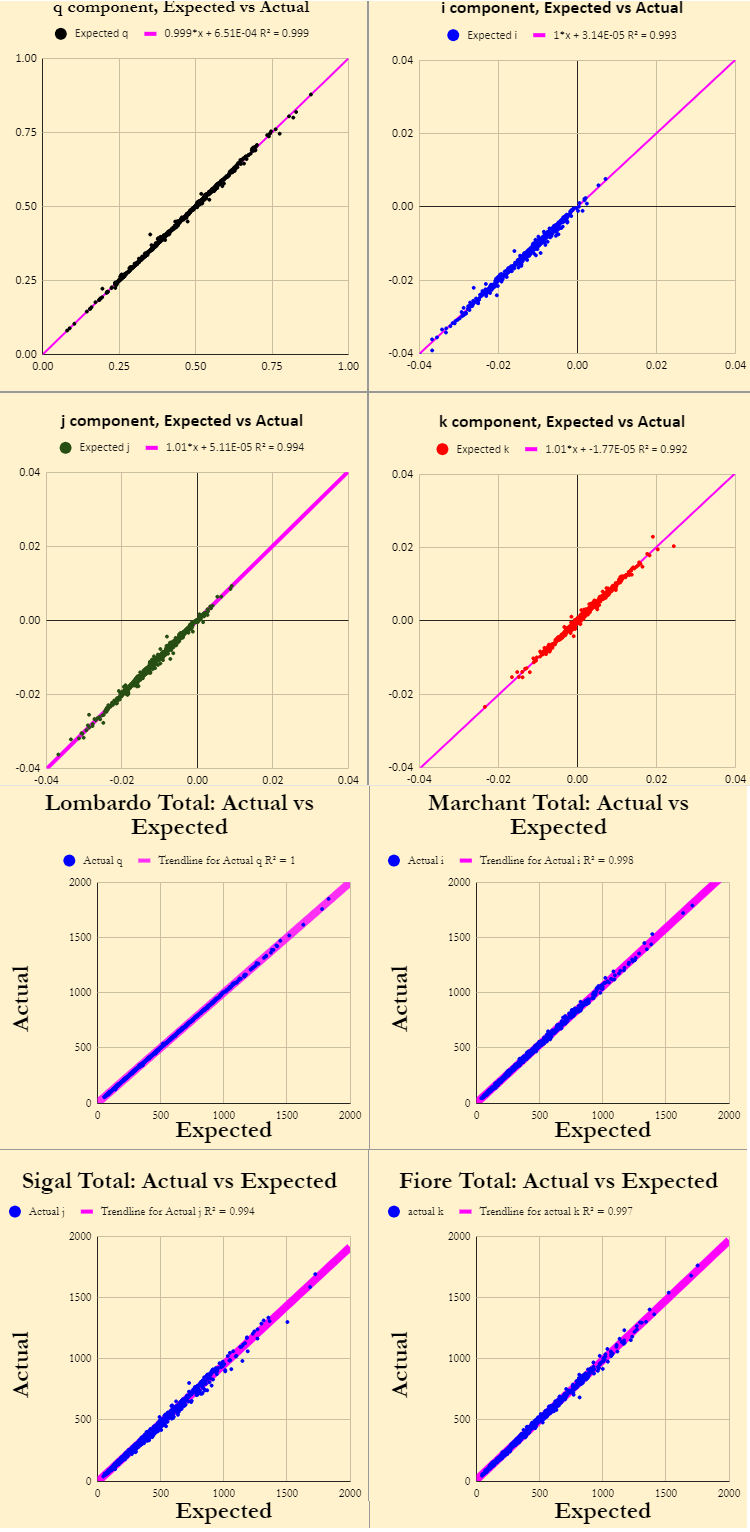
\includegraphics[width=300pt]{quaternionvotetotals.png}}
\end{center}
\end{figure}
\newpage
Now let's discuss the three key features of this formula, the three features that they thought would protect them from being discovered.
$$\vec{\alpha}_b=\vec{c}_{0}+\vec{g}_{b}\vec{c}_{1}+\vec{h}_{b}\vec{c}_{2}+\vec{g}_{b}\vec{c}_{3}\vec{g}_{b}+\vec{g}_{b}\vec{c}_{4}\vec{h}_{b}+\vec{h}_{b}\vec{c}_{5}\vec{g}_{b}+\vec{h}_{b}\vec{c}_{6}\vec{h}_{b}$$

The first feature is the most obvious: They used the West vs East Paradigm. They know that no one would ever think to consider the West and East percentages. Remember that I only discovered them by accident by placing Biden's Mail-in Vote in his Election Day column (and vice versa).

The second feature is that it's Quaternion of four races. In the event that someone discovered the West and East Side Percentages, they would still have to realize that they were dealing with a quaternionic of four races.

I was able to intuit that quaternions were involved when I found the manifold of Atlanta, Georgia, 2020 of Trump vs Biden, because the $g,h,\alpha$ real number manifold could not be solved directly from the $g,h,\alpha$ precinct coordinates, but rather had to first be rotated (I used Euler Angles at the time) before a regression of the rotated coordinates could faithfully return the original all three of the original $g,h,\alpha$ values with a high $R^2$ exceeding 0.99.

However, I did not know where the other quaternionic values came from in Atlanta (it never occurred to me at that time that they came from other races, as I was only analyzing the Trump vs Biden race in Atlanta)---so I kept it in mind.

When I discovered the Complex Number Manifold of two races for Trump vs Amodei in 2020 (Washoe), was when I connected the dots, and realized they were using quaternions to rig four races at a time. Which leads us to the third feature.

The third feature is that the third, fourth, fifth and sixth quadratic constants are sandwiched between the $x$ and $y$ vectors. They did this because one cannot simply perform ordinary least squares (that is multiply the Design Matrix by the conjugate transpose). 

In fact it was once thought impossible to to derive a ``Middle-Handed" constant via Least Squares. The paper titled \textit{An Iterative Algorithm for Least Squares Problem in Quaternionic Quantum Theory}, from the \textit{Computer Physics Communications, Volume 179, Issue 4, Pages 203-207}, was the best solution (and still a terrible one) at the time to handle the issue, which tried to converge upon (using a neural network) a local minimum solution magnitude error (via a residual cost function).
\newpage
Thus, it wasn't surprising to see that simply plugging in left or right handed constants against the quadratic terms failed to produce an faithful regression of the rigged elections, because they were rigged with Middle-Handed Constants. 

Not even the conniving ghouls that programmed the Middle-Handed Constants into the software knew how to back-solve their own rig via Quaternionic Least Squares. 

Thus, even if someone discovered both the West vs East Paradigm, and suspected a quaternionic setup of four races---they thought no one could ever get past their final obfuscation---the Middle-Handed Constants.

But I got them. And they're going to prison. Not even the best attorneys and ``experts" can defend a West vs East Quaternionic Manifold with Middle-Handed Constants that governs the vote proportions between the precincts of two counties on opposite sides of the State of Nevada--- and of Atlanta, of Michigan, of Pennsylvania, of Texas (Tarrant County), of Illinois, of Virginia, of Arizona, of Ohio, of Arkansas, of Tennessee...of EVERY STATE IN THE UNION ON AND AFTER November 3rd of 2020.

I am proud to say that I have saved my country from Quaternionic Election Fraud, for now Article 4, Section 4, of the United States Constitution must now be enforced:

\textit{The United States shall guarantee to every State in this Union a \textbf{Republican Form of Government}, and shall protect each of them against Invasion; and on Application of the Legislature, or of the Executive (when the Legislature cannot be convened) against domestic Violence.}

Without fair elections, we no longer have a Republican Form of Government. God Bless America.
\newpage


